%%%%%%%%%%%%%%%%%%%%%%%%%%%%%%%%%%%%%%%%%
% Masters/Doctoral Thesis 
% LaTeX Template
% Version 2.5 (27/8/17)
%
% This template was downloaded from:
% http://www.LaTeXTemplates.com
%
% Version 2.x major modifications by:
% Vel (vel@latextemplates.com)
%
% This template is based on a template by:
% Steve Gunn (http://users.ecs.soton.ac.uk/srg/softwaretools/document/templates/)
% Sunil Patel (http://www.sunilpatel.co.uk/thesis-template/)
%
% Template license:
% CC BY-NC-SA 3.0 (http://creativecommons.org/licenses/by-nc-sa/3.0/)
%
%%%%%%%%%%%%%%%%%%%%%%%%%%%%%%%%%%%%%%%%%

%----------------------------------------------------------------------------------------
%	PACKAGES AND OTHER DOCUMENT CONFIGURATIONS
%----------------------------------------------------------------------------------------

\documentclass[
11pt, % The default document font size, options: 10pt, 11pt, 12pt
%oneside, % Two side (alternating margins) for binding by default, uncomment to switch to one side
english, % ngerman for German
%singlespacing, % Single line spacing, alternatives: onehalfspacing or doublespacing
onehalfspacing, % Single line spacing, alternatives: onehalfspacing or doublespacing
%doublespacing, % Single line spacing, alternatives: onehalfspacing or doublespacing
%draft, % Uncomment to enable draft mode (no pictures, no links, overfull hboxes indicated)
nolistspacing, % If the document is onehalfspacing or doublespacing, uncomment this to set spacing in lists to single
%liststotoc, % Uncomment to add the list of figures/tables/etc to the table of contents
%toctotoc, % Uncomment to add the main table of contents to the table of contents
%parskip, % Uncomment to add space between paragraphs
%nohyperref, % Uncomment to not load the hyperref package
headsepline, % Uncomment to get a line under the header
%chapterinoneline, % Uncomment to place the chapter title next to the number on one line
consistentlayout, % Uncomment to change the layout of the declaration, abstract and acknowledgements pages to match the default layout
]{MastersDoctoralThesis} % The class file specifying the document structure

\usepackage[utf8]{inputenc} % Required for inputting international characters
\usepackage[T1]{fontenc} % Output font encoding for international characters

\usepackage{amsthm}
\usepackage{amsfonts}
\usepackage{amsmath}
\usepackage{algorithm,algorithmic}
\usepackage{booktabs}
\usepackage{breakcites}
\usepackage[autostyle=true]{csquotes} % Required to generate language-dependent quotes in the bibliography
\usepackage{enumitem}
\usepackage{graphicx}
\usepackage{layout}
\usepackage{mathtools}
\usepackage{multicol}
\usepackage{multirow}
\usepackage{subcaption}
\usepackage{hyperref}

%----------------------------------------------------------------------------------------
%	MARGIN SETTINGS
%----------------------------------------------------------------------------------------

\geometry{
	paper=a4paper, % Change to letterpaper for US letter
	inner=2.5cm, % Inner margin
	outer=3.8cm, % Outer margin
	bindingoffset=.5cm, % Binding offset
	top=1.5cm, % Top margin
	bottom=1.5cm, % Bottom margin
	%showframe, % Uncomment to show how the type block is set on the page
}

%----------------------------------------------------------------------------------------
%	CUSTOM COMMANDS
%----------------------------------------------------------------------------------------

% Set counter for subsubsections
\setcounter{tocdepth}{2}
\setcounter{secnumdepth}{3}

% Hypothesis and subhypothesis counters
\newcounter{hypothesis}
\renewcommand\thehypothesis{\Roman{hypothesis}}
\newcommand\hypothesisname{Hypothesis}
\newenvironment{hypothesis}[1][]
  {\refstepcounter{hypothesis}
    \par\medskip
    \noindent \textbf{\hypothesisname~\thehypothesis #1}
  \rmfamily\begin{em}}{\end{em}\medskip}

\newcounter{subhypothesis}[hypothesis]
\renewcommand\thesubhypothesis{\arabic{hypothesis}.\arabic{subhypothesis}}
\newcommand\subhypothesisname{Subhypothesis}
\newenvironment{subhypothesis}[1][]
  {\refstepcounter{subhypothesis}
    \par\medskip
    \textbf{\subhypothesisname~\thesubhypothesis #1}
  \rmfamily\begin{em}}{\end{em}\medskip}

% Definitions counter
\newcounter{definition}[chapter]
\renewcommand\thedefinition{\thechapter.\arabic{definition}}
\newcommand\definitionname{Definition}
\newenvironment{definition}[1][]
  {\refstepcounter{definition}
    \par\medskip
    \noindent \textbf{\definitionname~\thedefinition. #1}
  \rmfamily}{\medskip}

% Example environment
\newcounter{example}[chapter]
\renewcommand\theexample{\thechapter.\arabic{example}}
\newcommand\examplename{Example}
\newenvironment{example}[1][]
  {\refstepcounter{example}
    \par\medskip
    \noindent \textbf{\examplename~\theexample. #1}
  \rmfamily}{\medskip}

% Experiment environment
\newcounter{experiment}[chapter]
\renewcommand\theexperiment{\thechapter.\arabic{experiment}}
\newcommand\experimentname{Experiment}
\newenvironment{experiment}[1][]
  {\refstepcounter{experiment}
    \par\medskip
    \noindent \textbf{\experimentname~\theexperiment. #1}
  \rmfamily}{\medskip}

% Experiment enumeration
\newenvironment{enumexp}
  {\begin{enumerate}[label=\textbf{\theexperiment\alph*},ref=\theexperiment\alph*]}
  {\end{enumerate}}

% Metric environment
\newcounter{metric}
\renewcommand\themetric{\arabic{metric}}
\newcommand\metricname{Metric}
\newenvironment{metric}[1][]
  {\refstepcounter{metric}
    \par\medskip
    \noindent \textbf{\metricname~\themetric. #1}
  \rmfamily}{\medskip}

% Metric enumeration
\newenvironment{enummet}
  {\begin{enumerate}[label=\textbf{\themetric\alph*},ref=\themetric\alph*]}
  {\end{enumerate}}

% ABBREVIATION COMMANDS

\newcommand{\digito}{\textsc{digito}}
\newcommand{\nlp}{natural language processing}
\newcommand{\vsd}{verb sense disambiguation}
\newcommand{\wsd}{word sense disambiguation}

%----------------------------------------------------------------------------------------
%	THESIS INFORMATION
%----------------------------------------------------------------------------------------

\thesistitle{A Study on Semi-Supervised Methods for Spanish Verb Sense
Disambiguation} % Your thesis title, this is used in the title and abstract, print it elsewhere with \ttitle
\supervisor{Dra. Laura \textsc{Alonso Alemany}} % Your supervisor's name, this is used in the title page, print it elsewhere with \supname
\examiner{} % Your examiner's name, this is not currently used anywhere in the template, print it elsewhere with \examname
\degree{Doctor of Philosophy} % Your degree name, this is used in the title page and abstract, print it elsewhere with \degreename
\author{Cristian \textsc{Cardellino}} % Your name, this is used in the title page and abstract, print it elsewhere with \authorname
\addresses{} % Your address, this is not currently used anywhere in the template, print it elsewhere with \addressname

\subject{Computer Sciences Sciences} % Your subject area, this is not currently used anywhere in the template, print it elsewhere with \subjectname
\keywords{} % Keywords for your thesis, this is not currently used anywhere in the template, print it elsewhere with \keywordnames
\university{\href{https://www.unc.edu.ar/}{Universidad Nacional de C\'ordoba}} % Your university's name and URL, this is used in the title page and abstract, print it elsewhere with \univname
\department{\href{https://cs.famaf.unc.edu.ar/}{Secci\'on de Ciencias de la Computaci\'on}} % Your department's name and URL, this is used in the title page and abstract, print it elsewhere with \deptname
\group{\href{http://pln.famaf.unc.edu.ar/}{Grupo de Procesamiento de Lenguaje Natural}} % Your research group's name and URL, this is used in the title page, print it elsewhere with \groupname
\faculty{\href{http://www.famaf.unc.edu.ar/}{Facultad de Matem\'atica, Astronom\'ia, F\'isica y Computaci\'on}} % Your faculty's name and URL, this is used in the title page and abstract, print it elsewhere with \facname

\AtBeginDocument{
\hypersetup{pdftitle=\ttitle} % Set the PDF's title to your title
\hypersetup{pdfauthor=\authorname} % Set the PDF's author to your name
\hypersetup{pdfkeywords=\keywordnames} % Set the PDF's keywords to your keywords
}

\begin{document}

\frontmatter % Use roman page numbering style (i, ii, iii, iv...) for the pre-content pages

\pagestyle{plain} % Default to the plain heading style until the thesis style is called for the body content

%----------------------------------------------------------------------------------------
%	TITLE PAGE
%----------------------------------------------------------------------------------------

\begin{titlepage}
\begin{center}

{\scshape\LARGE \univname\\\facname\par}\vspace{0.5cm} % University name

\includegraphics[scale=0.4]{images/logounc.jpg}\\[0.4cm] % University/department logo - uncomment to place it
\textsc{\Large Doctoral Thesis}\\[0.2cm] % Thesis type

\HRule \\[0.4cm] % Horizontal line
{\huge \bfseries \ttitle\par}\vspace{0.4cm} % Thesis title
\HRule \\[1cm] % Horizontal line
 
\begin{minipage}[t]{0.4\textwidth}
\begin{flushleft} \large
\emph{Autor:}\\
\href{https://crscardellino.github.io}{\authorname} % Author name - remove the \href bracket to remove the link
\end{flushleft}
\end{minipage}
\begin{minipage}[t]{0.4\textwidth}
\begin{flushright} \large
\emph{Directora:} \\
\href{https://cs.famaf.unc.edu.ar/~laura/}{\supname} % Supervisor name - remove the \href bracket to remove the link  
\end{flushright}
\end{minipage}\\[1cm]

\large \textit{Trabajo de tesis presentado para obtener el título de\\  \degreename}\\[0.2cm] % University requirement text
\textit{en el}\\[0.2cm]
\groupname\\[0.5cm]%\deptname\\\facname\\[0.5cm] % Research group name and department name

{\large 20 de Abril de 2018}\\[0.5cm] % Date


\includegraphics[scale=0.75]{images/cc-by-sa.png}\\
{\small This work is licensed under
\href{http://creativecommons.org/licenses/by-sa/4.0/}{Licencia Creative Commons Atribución-CompartirIgual 4.0 Internacional.}}

% \vspace*{.06\textheight}
% {\scshape\LARGE \univname\par}\vspace{1.5cm} % University name
% \textsc{\Large Doctoral Thesis}\\[0.5cm] % Thesis type

% \HRule \\[0.4cm] % Horizontal line
% {\huge \bfseries \ttitle\par}\vspace{0.4cm} % Thesis title
% \HRule \\[1.5cm] % Horizontal line
 
% \begin{minipage}[t]{0.4\textwidth}
% \begin{flushleft} \large
% \emph{Author:}\\
% \href{http://crscardellino.me}{\authorname} % Author name - remove the \href bracket to remove the link
% \end{flushleft}
% \end{minipage}
% \begin{minipage}[t]{0.4\textwidth}
% \begin{flushright} \large
% \emph{Supervisor:} \\
% \href{https://cs.famaf.unc.edu.ar/~laura/}{\supname} % Supervisor name - remove the \href bracket to remove the link  
% \end{flushright}
% \end{minipage}\\[3cm]
 
% \vfill

% \large \textit{A thesis submitted in fulfillment of the requirements\\ for the degree of \degreename}\\[0.3cm] % University requirement text
% \textit{in the}\\[0.4cm]
% \groupname\\\deptname\\[2cm] % Research group name and department name
 
% \vfill

% {\large April 20, 2018}\\[4cm] % Date
% %\includegraphics{Logo} % University/department logo - uncomment to place it
 
\vfill
\end{center}
\end{titlepage}

\cleardoublepage

%----------------------------------------------------------------------------------------
%	DECLARATION PAGE
%----------------------------------------------------------------------------------------

% \begin{declaration}
% \addchaptertocentry{\authorshipname} % Add the declaration to the table of contents
% \noindent I, \authorname, declare that this thesis titled, \enquote{\ttitle}
% and the work presented in it are my own. I confirm that:
% 
% \begin{itemize} 
%   \item This work was done wholly or mainly while in candidature for a research
%     degree at this University.
%   \item Where any part of this thesis has previously been submitted for a
%     degree or any other qualification at this University or any other
%     institution, this has been clearly stated.
%   \item Where I have consulted the published work of others, this is always
%     clearly attributed.
%   \item Where I have quoted from the work of others, the source is always
%     given. With the exception of such quotations, this thesis is entirely my
%     own work.
%   \item I have acknowledged all main sources of help.
%   \item Where the thesis is based on work done by myself jointly with others, I
%     have made clear exactly what was done by others and what I have contributed
%     myself.\\
% \end{itemize}
%  
% \noindent Signed:\\
% \rule[0.5em]{25em}{0.5pt} % This prints a line for the signature
%  
% \noindent Date:\\
% \rule[0.5em]{25em}{0.5pt} % This prints a line to write the date
% \end{declaration}
% 
%\cleardoublepage

%----------------------------------------------------------------------------------------
%	QUOTATION PAGE
%----------------------------------------------------------------------------------------

\vspace*{0.2\textheight}

\noindent\enquote{\itshape The aim of a PhD's to ensure that no one, including
your advisor, understands what you're doing after the first couple of
years.}\bigbreak

\hfill China Mi\'eville

%----------------------------------------------------------------------------------------
%	ABSTRACT PAGE
%----------------------------------------------------------------------------------------

\begin{abstract}
  \addchaptertocentry{\abstractname} % Add the abstract to the table of contents

  \vspace{-1em}

  This thesis explores the use of {\em semi-supervised learning techniques for
  Spanish \vsd}. The objective is to study how information from unlabeled
  sources, which are larger, can help a classifier trained from a small labeled
  resource.

  Word sense disambiguation is a crucial task for many applications, like
  machine translation or information extraction. However, it is still an open
  problem, specially \vsd, due to the inherent complexity of verb senses.
  This, plus the fact that Spanish is a language with less resources than
  English, makes Spanish \vsd~an interesting area of study to contribute.

  First I obtain a thorough understanding of purely supervised models and their
  weaknesses. I find that the main shortcomings of the supervised approach are
  lack of coverage and tendency to overfit. I try to overcome these problems
  with different semi-supervised techniques.

  Then, I explore the use of {\em word embeddings} as unsupervised
  representations within supervised classifiers. This approach is known as {\em
  disjoint semi-supervised learning}: an unsupervised technique is used prior
  to a supervised one to aid the latter. Word embeddings help to overcome lack
  of coverage and tendency to overfit, even if at the expense of losing some
  performance in other aspects, like accuracy or F1-score.

  I continue with the exploration self-learning, a {\em joint semi-supervised
  learning} algorithm that uses a supervised classifier, trained on an initial
  labeled dataset, to select instances from a pool of unlabeled data. Using
  some measure of certainty, it annotates those instances for which the
  algorithm has the highest confidence and uses them to expand the labeled data
  to re-train the supervised classifier. I found that self-learning suffers
  strongly from unbalanced datasets. It amplifies the bias toward the most
  frequent class, so the expected increase in coverage by adding new examples
  to training is shaded because decision boundaries between classes are
  blurred.

  Complementary to self-learning, I explore {\em active learning}. This
  approach uses a supervised model to select instances taken from a pool of
  unlabeled data, based on the impact these will have in the model, and gives
  them to a human expert to annotate. I show that information obtained via
  active learning, although little in comparison, can outperform the
  self-learning approach.

  Finally, I explore {\em ladder networks}, a neural network which minimizes a
  combined cost function. This cost function is a sum of a supervised cost
  function and an unsupervised cost function, thus overcoming the tendency to
  overfit of supervised models. Also, the method's performance is shown to be
  comparable or better to the rest of methods presented on this thesis, making
  the ladder network an interesting candidate for semi-supervised learning.
\end{abstract}

%----------------------------------------------------------------------------------------
%	ACKNOWLEDGEMENTS
%----------------------------------------------------------------------------------------

\begin{acknowledgements}
\addchaptertocentry{\acknowledgementname} % Add the acknowledgements to the table of contents

  Esta tesis es fruto del trabajo y la ayuda de más gente que la que pueda 
  nombrar en una sóla página. Pero haré lo posible para agradecer a todos los
  que participaron en esta travesía.

  Empezaré por mi familia, la que me vió crecer desde chico pero también esa
  que formé. Mis viejos, Liliana y Oclides, que tanto me apoyaron y me bancaron
  (y nunca dejaron de hacerlo). Ellos son los responsables de que haya elegido
  este camino del estudio, porque desde muy chico me inculcaron la pasión por
  el aprendizaje y el conocimiento, por la curiosidad y la imaginación. Fueron
  mis padres los que me insistieron que la educación es el único camino a la
  verdadera libertad, tanto física como metafísica. Me enseñaron la disciplina
  de sentarme a estudiar y saber esforzarme para lograr mis objetivos. Gracias
  a su educación tengo hoy en día la integridad con la que pude lograr mis
  metas.  También le agradezco a mi hermano Fernando que, aunque de vez en
  cuando peleamos, sé que en él siempre hay un oído confiable y una voz
  razonable que me puede escuchar y aconsejar.  

  A Vale y a Cami (y a la Pelu y al Tito), que me dieron una familia y con las
  que he formado un hogar al cuál volver cada día, son la familia por la cuál
  vale la pena mejorar cada día y buscar superarme más allá de mis límites.
  Ellas que me soportan el día a día, en las buenas y las malas, siempre
  preocupadas por que esté bien y que no me falte nada. Es por ellas que busco
  todos los días ser la mejor versión de mi mismo, son mi razón para vivir y
  nunca me van a alcanzar las palabras para agradecer todo el cariño que me han
  dado y me dan cada día. Espero que esto sea el inicio de una nueva etapa que
  pueda compartir con ellas y aprovechar lo que aprendí para devolverles a
  ellas todo el afecto que merecen y más aún la vida y las oportunidades para
  que ambas puedan lograr sus sueños. Gracias chicas, este trabajo está
  dedicado a ustedes. También no quería dejar de agradecerles a mis suegros,
  Esther y Jorge, que siempre, junto a mis viejos, nos han ayudado y brindado
  consejos en esto nuevo para mi que es la vida con mi familia.

  Agradezco a mis amigos, que a lo largo de mis años han sido muchos y muy
  buenos.  Compañeros de historias y anécdotas inolvidables. Con los que he
  vivido miles de situaciones entrañables y con los que compartí risas y buenos
  momentos.  Juntarse con ellos y pasar un buen rato hablando, jugando o
  simplemente matando el tiempo es algo que no tiene precio.  Tanto aquellos
  viejos amigos de toda la vida que conozco desde pequeño como los excelentes
  compañeros que conocí en mis años de facultad, es un privilegio haber
  compartido con todos ustedes una etapa tan importante de mi vida. Gracias a
  todos por su buena onda, muchas gracias de verdad.

  Profesores y maestros, muchos más de los que puedo nombrar, desde el jardín
  de infantes hasta la universidad, todos aquellos que me brindaron su
  sabiduría y conocimiento. Gracias a todos por su esfuerzo, por brindarme las
  herramientas para ser libre, puesto que sin el conocimiento la libertad es
  simplemente una idea vacía.

  A mis compañeros del doctorado, los muchachos de la oficina 272: José, Luis,
  Mariano y Raúl, que me acompañaron en estos años, siempre dispuestos a dar
  una mano en todo lo que podían y con los que siempre pasamos un buen momento
  en las comilonas que hacemos. Gracias por todo muchachos, ha sido un honor
  compartir con ustedes estos años de doctorado.

  A mis colegas de la facultad, tanto los docentes como investigadores.
  Especialmente a los miembros del grupo de procesamiento de lenguaje natural y
  el grupo de terapia con el que siempre puedo contar para obtener buen
  feedback sobre mi trabajo.

  A los miembros del jurado de mis tesis de doctorado: Jorge, Marcelo y Paula.
  Gracias por su tiempo, gracias por sus ganas y gracias por haber sido parte
  de esto tan importante que fue mi tesis doctoral.

  Por último quiero agradecer a mis dos compañeras de oficina y también de
  investigación, que hacen el día a día en la facultad divertido, interesante y
  genial. Mili, mi hermana académica, ha sido un privilegio tener a alguien tan
  activa, alegre y positiva, siempre brindando consejos, siempre dispuesta a
  debatir y otorgar su visión para ayudar a comprender estas cosas complejas
  que estudiamos, una compañera de trabajo excelente con la que hemos logrado
  sinergizar en varios proyectos tanto académicos como docentes, y una amiga
  extraordinaria con quien puedo contar.

  Y Laura, mi madre académica, mi supervisora y mentora en este viaje que ha
  sido el doctorado. A vos te debo este logro más que a nadie, por apoyarme y
  guiarme, por nunca bajar los brazos y estar siempre dispuesta a darme toda la
  ayuda que necesitara, tanto en tus mejores como en tus peores momentos. Nunca
  me impusiste tu visión o tu agenda y siempre me animaste a seguir adelante,
  cualquiera fuera el tema de investigación que quisiera explorar. Más allá de
  eso siempre te las arreglaste para darme los contactos y las herramientas
  para avanzar profesionalmente y lograr todos mis objetivos. Es gracias a vos
  que logré formarme como lo hice. Fue mi privilegio y mi honor ser tu
  doctorando. Muchas gracias por todo Laura.

\end{acknowledgements}

%----------------------------------------------------------------------------------------
%	LIST OF CONTENTS/FIGURES/TABLES PAGES
%----------------------------------------------------------------------------------------

\tableofcontents % Prints the main table of contents

\listoffigures % Prints the list of figures

% \listoftables % Prints the list of tables

%----------------------------------------------------------------------------------------
%	ABBREVIATIONS
%----------------------------------------------------------------------------------------

% \begin{abbreviations}{ll} % Include a list of abbreviations (a table of two columns)
% 
% \textbf{LAH} & \textbf{L}ist \textbf{A}bbreviations \textbf{H}ere\\
% \textbf{WSF} & \textbf{W}hat (it) \textbf{S}tands \textbf{F}or\\
% 
% \end{abbreviations}

%----------------------------------------------------------------------------------------
%	PHYSICAL CONSTANTS/OTHER DEFINITIONS
%----------------------------------------------------------------------------------------

% \begin{constants}{lr@{${}={}$}l} % The list of physical constants is a three column table
% 
% % The \SI{}{} command is provided by the siunitx package, see its documentation for instructions on how to use it
% 
% Speed of Light & $c_{0}$ & \SI{2.99792458e8}{\meter\per\second} (exact)\\
% %Constant Name & $Symbol$ & $Constant Value$ with units\\
% 
% \end{constants}

%----------------------------------------------------------------------------------------
%	SYMBOLS
%----------------------------------------------------------------------------------------

% \begin{symbols}{lll} % Include a list of Symbols (a three column table)
% 
% $a$ & distance & \si{\meter} \\
% $P$ & power & \si{\watt} (\si{\joule\per\second}) \\
% %Symbol & Name & Unit \\
% 
% \addlinespace % Gap to separate the Roman symbols from the Greek
% 
% $\omega$ & angular frequency & \si{\radian} \\
% 
% \end{symbols}

%----------------------------------------------------------------------------------------
%	DEDICATION
%----------------------------------------------------------------------------------------

\dedicatory{Dedicado a toda mi famila\ldots Gracias por todo\ldots} 

%----------------------------------------------------------------------------------------
%	THESIS CONTENT - CHAPTERS
%----------------------------------------------------------------------------------------

\mainmatter % Begin numeric (1,2,3...) page numbering

\pagestyle{thesis} % Return the page headers back to the "thesis" style

\part{Preliminaries} 

\chapter{Introduction}\label{chapter:introduction}
\section{Overview}\label{section:introduction:overview} 

This thesis explores the use of semi-supervised learning techniques for Spanish
\vsd. The objective is to study how adding information from unlabeled sources,
which are larger, can help a classifier learned from a labeled but small
resource, as is the disambiguated corpus for Spanish verbs SenSem
\cite{alonso-etal-07-sensem}.

{\em Supervised machine learning} is the task that infers a function that maps
unlabeled data to a label. This function is inferred from labeled data, which
have been manually associated to a label. This is also known as modeling of the
data.  This function can be used then to find new mappings given unseen
examples. However, supervised learning models are limited by the amount of
labeled data available. The more labeled data a model has, the better the
performance of the model. Right now {\em deep learning} requires large amounts
of data in order to generate good models. As data labeling is a task requiring
human labor, having large enough datasets is generally expensive. This is also
dependent on the task. Some tasks are relatively easy for any person to label
(e.g. see if a picture has a cat in it). For other tasks, labeled data is more
difficult to obtain, as it requires that the human annotators are domain
experts (e.g. a lawyer, a physician, a linguist, etc.).

{\em Unsupervised machine learning} is the task that tries to find patterns or
hidden structures in unlabeled data. Because the data are unlabeled, these
patterns cannot be evaluated based on accuracy. Unsupervised machine learning
is more centered in the exploration of the data rather than finding a function
useful for a particular prediction task, like supervised learning. The
advantage of unsupervised learning is the vast amount of data available. As the
data is not annotated, it makes it cheap to gather datasets.

{\em Semi-supervised learning} is an approach in between. A semi-supervised
algorithm makes use of both labeled and unlabeled data in order to better infer
a function for a specific task (whether it is supervised or not). In this case,
given enough data, a good semi-supervised learning technique can improve on the
purely supervised or unsupervised algorithm it is using. In particular, it has
the advantage of having a way to evaluate it in means of accuracy or other
metrics, but also has the advantage of being able to expand its models based on
the cheap available unlabeled datasets. The objective of this thesis is to
explore different semi-supervised models in order to improve on a supervised
task which has the properties stated above: lack of large labeled datasets, but
availability of large unlabeled datasets.

{\em Natural language processing} helps humans interact with machines using the
human language, instead of a formal language. The main challenge of the area is
the ambiguity of human language. But this is not the only problem. Human
language, as many other social phenomena, has a Zipfian distribution
\cite{j:zpf}, which is an exponential distribution. This law states that given
a corpus of natural language utterances, the frequency of any word is inversely
proportional to its rank in the frequency table. Thus, the most frequent word
will occur approximately twice as often as the second most frequent word, three
times as often as the third most frequent word, etc. In the case of
classification tasks of natural language processing, the classes are unbalanced
following Zipf's law, thus very few classes occur very often, and the rest of
them have few to no occurrences in the labeled dataset. As with everything, the
availability of good models for natural language tasks depends on the data
available for that task. In particular, different languages have different
amount of data, thus making it possible to obtain better or worse models. E.g,
English is language with very good models because of the amount of resources;
other languages are harder to work with because there are less available
resources.

{\em Word sense disambiguation} is an intermediate task of natural language
processing which, as it names indicates, given a word and its context tries to
discriminate the meaning of that word among an inventory of pre-determined
senses. E.g. the noun ``granada'' can be a fruit or a weapon depending on the
context it is used in. A sub-task of \wsd~is {\em \vsd}, which is crucial for a
deep language processing tasks, especially those that could benefit from
information about relations between participants provided by the verb, like
machine translation, question answering or information extraction. E.g., in
machine translation, sense disambiguation is needed to determine the correct
translation of a word, and also the transformations needed in the syntactical
structure of the sentence. Examples \ref{example:hacer:1} and
\ref{example:hacer:2} shows how the different senses can change the translation
of the same word.

\begin{example}\label{example:hacer:1}
  \begin{itemize}
    \item Juan {\bf hizo} una torta de chocolate.
    \item {\em Juan {\bf made} a chocolate cake.}
  \end{itemize}
\end{example}

\begin{example}\label{example:hacer:2}
  \begin{itemize}
    \item Juan {\bf hizo} la tarea por la tarde.
    \item {\em Juan {\bf did} the homework in the afternoon.}
  \end{itemize}
\end{example}

Another example, for question answering over linked data \vsd~is needed to
determine the sense of a verb and the logical relations between the
participants to access the adequate nodes and edges in an ontology. Examples
\ref{example:acceder:1} and \ref{example:acceder:2} show how the same verb has
different connotations and thus establish different relationships between the
participants it connects.

\begin{example}\label{example:acceder:1}
  \begin{itemize}
    \item El investigador no pudo {\bf acceder} a la informaci\'on reservada.
  \end{itemize}
\end{example}

\begin{example}\label{example:acceder:2}
  \begin{itemize}
    \item Pedro {\bf accedi\'o} a escribir una nota de descargo.
  \end{itemize}
\end{example}

Finally, an information extraction task like relation extraction where \vsd~is
needed to disambiguate those relationships, generally represented as verbs in a
unstructured text.

However, \vsd~is a highly difficult task, that achieves even lower precision
rates than \wsd~for other morphosyntactic categories (nouns, adjectives). This
is arguably due to the inherent complexity of verb senses and the fact that
their meaning is more pervasive than that of nouns, thus making it more
difficult to discretize \cite{chen2009improving}.  Find below a detailed
example of verb sense ambiguity for the lemma {\emph hablar}, with five senses
in the SenSem lexicon. This can be seen in example \ref{example:hablar:1}.

\begin{example}\label{example:hablar:1}
  \begin{itemize}
    \item (...) una joven realizadora irlandesa que (...) {\bf habla}
      castellano con acento malague\~no ya que de peque\~na vivi\'o tres a\~nos
      en Estepona.
  \end{itemize}
\end{example}

\begin{example}\label{example:hablar:2}
  \begin{itemize}
    \item El presidente del Gobierno (...) {\bf hablar\'a} con las principales
      autoridades de ambos estados sobre las perspectivas de la Uni\'on Europea
      (...).
  \end{itemize}
\end{example}

In Example \ref{example:hablar:1} {\it hablar} is a state with the meaning of
``being able to speak a language'', while in example \ref{example:hablar:2} it
is a process with the meaning ``talk''. The subcategorization frames of each
sense are also very different: for the first, we have two themes, while the
second has the typical communication frame, with an Agent-Origin, a Theme and a
Goal-Receiver.

\section{Contributions and outline of this thesis}\label{section:outline}

Word sense disambiguation is still an open problem in the area of natural
language processing. Many different techniques and algorithms have been
researched to attack this problem. Methods range from the use of lanaguage
resources and knowledge databases, dictionary-based, rule-based, supervised
machine learning and even purely unsupervised techniques that seek to infer
senses by word clustering. There are even hybrid methods which are a
combination of these. Supervised machine learning techniques are based on
corpora of disamgibuated words. Given this one can train a classifier to
recognize senses in unseen examples.

Most of the work for Spanish \wsd~is not specifically for verbs. Much of the
work is using knowledge bases
\cite{Agirre:2014:RWK:2645242.2645245,Agirre:2009:PPW:1609067.1609070}. There
is some work using supervised learning techniques or unsupervised learning
techniques \cite{MihalceaEtAl2004}. But at the time of writing this thesis, the
work done specifically for Spanish \vsd~using the semi-supervised techniques
explored in this work is non-existent to my knowledge. Moreover, the work in
this thesis is using a resource that, save for the publications that derived in
this thesis, has not been explored. I use as my basic resource the corpus of
disambiguated verbs SenSem \cite{alonso-etal-07-sensem}.

This resource, although valuable as it was annotated by domain experts, is very
small an has a limited amount of examples. But there is a large amount of
unlabeled corpora available on the internet for Spanish (e.g. the SBWCE corpus
\cite{cardellinoSBWCE}). This gives me the opportunity to study semi-supervised
techniques applied to a problem that could really benefit from it, rather than
a generic problem based on a toy dataset with properties that real world data
might lack. Likewise, by studying the impact of semi-supervised machine
learning techniques for Spanish \vsd~rather than for English \vsd, I contribute
to the improvement of NLP for a language whose resources are less developed.
The main contribution of this thesis can be summarized in the study of how
different semi-supervised systems overcome the problems of Spanish \vsd.

The two following chapters introduce the fundamental concepts and related work
of this thesis. Chapters \ref{chapter:general_background} and
\ref{chapter:domain_background} present a background review of the two main
ares of this thesis: {\em machine learning} and {\em natural language
processing}. Specifically Chapter \ref{chapter:general_background} introduces
the relevant concepts for the work in next chapters, and presents a brief
description and analysis of previous work for the semi-supervised learning
techniques studied in this thesis. Chapter \ref{chapter:domain_background} is a
background chapter on \nlp~and \wsd. It introduces the fundamental concepts of
the area and does a review of the previous work on supervised and
semi-supervised learning techniques applied specifically to the areas of
\nlp~and \vsd. The five core chapters of this thesis explore different
hypotheses for Spanish \vsd~and experiment and analyze results to test those
proposed hypotheses.  The final chapter recapitulates on the findings and
lessons learned of this thesis and describes lines for future work.

\paragraph{Summary of Chapter \ref{chapter:supervised}: Supervised Learning}

This chapter explores supervised machine learning techniques for \vsd. The main
objective is to establish a baseline. The chapter explores \vsd~both for
Spanish and English. The latter is needed as a comparison ground to ensure that
there is no language related bias. The chapter explores different
classification algorithms and representations given by {\em hand-crafted
features} to discard techniques that underperform. I also present a deep
discussion about the insight provided by metrics and their biases.  This is
needed for a thorough understanding of models and their weaknesses to properly
direct further developments. Finally, the chapter states the main shortcomings
of the supervised approach: lack of coverage and tendency to overfit. I try to
overcome these problems with the different semi-supervised techniques explored
in the thesis.

\paragraph{Summary of Chapter \ref{chapter:embeddings}: Word Embeddings}

This chapter explores the use of {\em word embeddings} as unsupervised
representations within supervised classifiers. This approach is known as {\em
disjoint semi-supervised learning}: an unsupervised technique is used prior to
a supervised one to aid the latter. The chapter explores how the domain of the
word embeddings affects the performance of the supervised classifiers, and how
word embeddings help to overcome lack of coverage and tendency to overfit,
even if at the expense of losing some performance in other aspects, like 
accuracy or F1.

\paragraph{Summary of Chapter \ref{chapter:self-learning}: Self-Learning}

This chapter explores the self-learning algorithm, a well established method
and one of the earliest semi-supervised algorithms in existence.  Self-learning
is a {\em wrapper algorithm}. The algorithm uses a supervised classifier,
trained on an initial labeled dataset, to select instances from a pool of
unlabeled data. Using some measure of certainty, it annotates those instances
for which the algorithm has the highest confidence and uses them to expand the
labeled data to re-train the supervised classifier. Experiments in this chapter
focus primarily on increasing the amount of labeled data available to train a
classifier. The final objective is to have a supervised model with a larger
coverage by integrating part of the unlabeled data into the training process,
assigning them a label automatically. Self-learning is the first of the {\em
joint semi-supervised learning} techniques explored in the thesis.  In this
type of algorithms the labeled and unlabeled data are used together in the
process of learning. I found that self-learning suffers strongly from
unbalanced datasets. It amplifies the bias toward the most frequent class, so
the expected increase in coverage by adding new examples to training is shaded
because decision boundaries between classes are blurred.

\paragraph{Summary of Chapter \ref{chapter:active}: Active Learning}

This chapter explores active learning as a semi-supervised approach. Active
learning is based on the same idea of self-learning. It is a wrapper algorithm
that uses a supervised model to select instances taken from a pool of unlabeled
data. However, instead of annotating the instances automatically, like
self-learning, it uses an {\em intelligent approach} to select data and gives
it to a human expert to annotate. The data is selected based on the impact it
will have in the model to correctly annotate it (e.g. by giving more
information to the model). As manual annotation is expensive, the idea is to
reduce the resources spent on annotation to a bare minimum. The chapter
experiments show that information obtained via active learning, although little
in comparison, can outperform the self-learning approach, which is generally
biased by the nature of language and Zipf's law.

\paragraph{Summary Chapter \ref{chapter:ladder}: Ladder Networks}

Finally, this chapter explores {\em ladder networks}. This is a novel approach
in the field of semi-supervised learning, which presents a neural network
architecture based on the idea of simultaneously training the weights of the
network by minimizing a combined cost function. This cost function is a sum of
a supervised cost function and an unsupervised cost function. The network
consists on two paths: an encoding path optimizing the supervised cost
function and a decoder path which reconstructs the encoding input layer by
layer. The idea is that the information gathered by the unsupervised path will
help the supervised approach to better generalize, thus overcoming the tendency
to overfit of supervised models. Also, the method's performance is shown to be
comparable or better to the rest of methods presented on this thesis, making
the ladder network an interesting candidate for semi-supervised learning.


\chapter{Machine Learning Background}\label{chapter:general_background}
The core of this thesis' work relies on two main areas: {\bf machine learning}
and {\bf \nlp}. More specifically, this thesis follows the application of
semi-supervised learning techniques, a subarea of machine learning, for {\bf
  Spanish \vsd}, a subarea of \nlp. This chapter reviews {\em machine
learning}, specifically semi-supervised learning. The chapter starts with a set
of basic definitions. It continues by revising the two wrapper algorithms:
self-learning and active learning. And finishes with a brief introduction to
the ladder network algorithm.

\section{Fundamental concepts}\label{sec:general_background:fundamental}

Tom Mitchell \cite{mitchell1997machine} defines {\bf machine learning} as ``the
field of artificial intelligence concerned with the question of how to
construct systems that automatically improve based on experience''. The
experience, in this case, is acquired through the analysis of data with the
final objective to generate a model that works on specific tasks. Examples of
these tasks can be systems for anomaly detection, like fraudulent credit card
transactions; recommender systems for movies, music, books, etc.; or computer
vision.

Machine learning is divided in three main areas: {\em supervised learning},
{\em unsupervised learning}, and {\em reinforcement learning}. As this work
is mostly based on supervised learning techniques with aid of unsupervised
learning ones, I will go ahead and describe them.

{\bf Supervised learning} has the objective to build a predictive model from
labeled data. {\bf Labeled data} consists in a set of {\em annotated examples},
where each is a pair of input data, generally a vector; and output data which,
depending on the task, can be a real number, for regression, or a categorical
value, for classification. E.g. spam filtering where an email is either
classified as spam or not. In more formal terms, a supervised learning
algorithm is a mapping from input $\mathbf{x}$ to output $\mathbf{y}$ with
target $t$, trained from a set of $N$ pairs: $\{(\textbf{x}(n), t(n)) | 1 \leq
n \leq N\}$.

{\bf Unsupervised learning} has the objective to describe or discover a hidden
structure from unlabeled data. {\bf Unlabeled data} consists in a set of {\em
unannotated examples}: data without any information about belonging to some
class or having an associated value. E.g. clustering of news articles. In more
formal terms, an unsupervised learning algorithm is the inference of a function
that describes some pattern or structure from a set of unlabeled data points:
$\{\textbf{x}(m) | 1 \leq m \leq M\}$.

There is a set of techniques which are in-between supervised and unsupervised
machine learning: {\bf semi-supervised machine learning}. These are the
techniques I mostly explore in this thesis. Zhu and Goldberg
\cite{zhu2009introduction} describe it as ``the task consisting in using both
annotated and unannotated examples in order to better learn an otherwise
supervised or unsupervised task''. For the objective of this thesis, I will
refer to semi-supervised techniques which explore the use of unlabeled data in
aiding a supervised model. In more formal terms, given a supervised model from
a training set of pairs $\{\textbf{x}(n), t(n) | 1 \leq n \leq N\}$.
Semi-supervised learning, in the scope of this thesis, studies how auxiliary
unlabeled data $\{\textbf{x}(n) | N + 1 \leq n \leq M\}$ can help in training
the supervised model. It is often the case that labeled data is little whereas
unlabeled data is plentiful, that is $N \ll M$. The idea is that unlabeled data
can help expanding the supervised model as it has more information than a
labeled dataset regarding the instances (since it has more). That underlying
information helps expand the information present in the model. The information
can be synthesized as new features for a class, latent variables coming from
the representations, stronger associations between features and classes, etc.

In this work I explore two types of semi-supervised learning: {\em disjoint
semi-supervised learning} and {\em joint semi-supervised learning}. In {\bf
disjoint semi-supervised learning} the supervised and unsupervised steps are
trained separately, and then the information from one is fed into the other to
improve it \cite{Weston2008}. E.g the use of {\em word embeddings} trained on
an unlabeled corpus for a supervised task. In contrast {\bf joint learning}
both supervised and unsupervised data affect the model training procedure
simultaneously. There can be another subdivision in joint learning methods.
Joint learning based on {\em wrapper} algorithms starts from a supervised
classifier trained on labeled data, and uses the information of that model to
expand it with feedback from unlabeled data (e.g. an {\em active learning}
approach which makes an ``intelligent'' selection of candidates gathered from
an unsupervised corpus to manually annotate and subsequently use to feed a
supervised model). Other joint learning algorithms use both the labeled and
unlabeled datasets in the training procedure of the algorithm ( e.g. {\em
ladder networks} learn by the minimization of a joint objective function,
composed by a supervised and an unsupervised target).

A categorization that can be done also in semi-supervised methods, but more
generally in supervised methods as well is: {\em shallow learning} and {\em
deep learning}. {\bf Shallow learning} can be described as a process that
tries to learn by approximation. It is rather a memorization rather than an
understanding of underlying concepts or structures of the data. {\bf Deep
learning} is a machine learning approach whose objective is to allow computers
to learn from experience and understand the world in terms of a hierarchy of
concepts, with each concept defined in terms of its relation to simple
concepts. By gathering knowledge from experience, this approach avoids the need
for human operators to formally specify all of the knowledge that the computer
needs. The hierarchy of concepts allows the computer to learn complicated
concepts by building them out of simpler ones
\cite{Goodfellow-et-al-2016-Book}. The most basic deep learning model is a {\bf
multilayer perceptron}, a feed-forward artificial neural network model, which
maps a set of input values to a set of output values. 

\section{Relevant work}\label{sec:general_background:relevant}

\subsection{Disjoint Semi-supervised Learning}

{\bf Disjoint semi-supervised learning} was defined by Weston et al.
\cite{Weston2008}, as the use of word embeddings to aid deep learning tasks in
\nlp. The concept can be understood as the use of a resource or an auxiliary
task that is obtained from unlabeled data (e.g. word embeddings) and how it
aids on a supervised task trained on labeled data that is disjoint the
unlabeled data of the auxiliary task. As it was defined, there are no other
uses of the term but inside the area of \nlp. Thus, I will discuss it further
on Chapter \ref{chapter:domain_background}.

\subsection{Self-learning}\label{sec:general_background:self-learning}

{\bf Self-learning} (also known as {\em self-training}, {\em self-teaching}, or
{\em bootstrapping}) is a commonly used technique for semi-supervised learning.
It is probably the earliest idea about using unlabeled data in classification
\cite{Chapelle:2010:SL:1841234}. This is a {\em wrapper} algorithm that
repeatedly uses a supervised learning method. The initial classifier is first
trained with a seed labeled dataset (generally small) and then is used to
classify data from an unlabeled pool of data. Generally the data points on
which the classifier is more confident about alongside their predicted labels
are added to the training set. The classifier is re-trained and the procedure
repeated. Note that the classifier uses its own predictions to teach itself
\cite{Zhu05}, thus in this scheme is possible for the classification mistake to
reinforce itself. There are different methods to try and control this
phenomenon. Scudder \cite{Scudder:2006:PEA:2263254.2267291} presents an
untaught adaptive pattern-recognition machine made from a simple taught
pattern-recognition machine for detecting an unknown, fixed, randomly occurring
pattern (derived using a Bayes' approach) and its probability of error is
analyzed by using its own output instead of a teacher. In machine vision,
Rosenberg et al. \cite{4129456} apply self-training to object detection systems
from images, and show the semi-supervised technique compares favorably with a
state-of-the-art detector. Culp and Michailidis
\cite{doi:10.1198/106186008X344748} offer an iterative self-learning algorithm
that extends a learner from a supervised setting to a semi-supervised one. They
analyze the convergence properties of the algorithm, as self-learning is a hard
algorithm to analyze in general.

\subsection{Active learning}\label{sec:general_background:active}

{\bf Active learning} is another example of a joint learning task. It is also a
wrapper algorithm which trains from an initial seed labeled dataset, but uses
another approach to incorporate instances from the unlabeled dataset. The key
hypothesis is that if the learning algorithm is allowed to choose the data from
which it learns it will perform better with less training \cite{settles.tr09}.
The algorithm inspects a set of unlabeled examples, and ranks them by how much
they could improve the algorithm's performance if they were labeled. Then, a
human annotator (called {\em oracle} or {\em domain expert}) labels the highest
ranking examples, which are then added to the set of training examples from
which the algorithm infers its classification model, and the loop begins again.
In some active learning approaches, the oracle may annotate features describing
instances, and not (only) instances themselves. This latter approach provides
even faster learning in some cases \cite{druck.emnlp09}.

Different strategies have been applied to determine the most useful instances
to be annotated by the oracle, including expected model change, expected error
reduction or density-weighted methods \cite{settles.tr09}. The most intuitive
and popular strategy is {\bf uncertainty sampling}
\cite{Lewis94heterogeneousuncertainty}, which chooses those instances or
features where the algorithm is most uncertain, from a large set of
automatically labeled data. As {\em self-training}, this is also a wrapper
method, being the supervised algorithm to do the classification step chosen
openly. This strategy has been successfully applied to Information Extraction
tasks \cite{Culotta:2005:RLE:1619410.1619452,settles.emnlp08}. Uncertainty can
be calculated by different methods depending on the learning algorithm.
Specially popular are methods exploiting the margins of Support Vector Machines
(SVM), as in \cite{Tong:2002:SVM:944790.944793}. The simplest methods exploit
directly the certainty that the classifier provides for each instance that is
classified automatically.

\subsection{Ladder Networks}

The {\bf ladder network} is the last semi-supervised learning technique I will
revise in this work. It is also a joint learning technique. But unlike
self-learning or active learning, it is not a wrapper algorithm, but rather an
special architecture for an artificial neural network. The semi-supervised
approach studied by the ladder network is recent, being introduced in the work
of Rasmus et al. \cite{Rasmus:2015aa}. I will further discuss this work and the
details of the ladder network algorithm in Chapter \ref{chapter:ladder}, since
the explanation of it is core of this thesis's work. The work of Rasmus extends
the original work by Valpola \cite{Valpola:2014aa} which introduces the concept
of ladder networks for unsupervised learning. The work of Rasmus that I study
in this thesis uses the basis of another work by Rasmus et al.
\cite{Rasmus:2015ab} which adds lateral connections to denoising autoencoders
to help supervised learning (e.g. classification) with an unsupervised learning
auxiliary task (e.g. reconstruction of input). The combination of works derived
in the design of a ladder network as a semi-supervised algorithm.


\chapter{Natural Language Processing
Background}\label{chapter:domain_background}
Besides machine learning, the other main area of study in this thesis is {\bf
\nlp}. In particular, I focus on a subarea of \nlp: {\bf \wsd}, with special
attention on {\bf Spanish \vsd}. This chapter reviews {\em \nlp} and {\em \wsd}
(with particular interest on {\em Spanish \vsd}). More specifically, it
explores some of the relevant work on \nlp~and \wsd~using the semi-supervised
learning techniques described in the previous chapter. The chapter first
describes the fundamental concepts of the area of \nlp~and \wsd. Then it
explains the details of word embeddings and their applications on \nlp. Finally
it continues with the revision of self-learning and active learning algorithms
in the area of \nlp. There is no previous work for ladder networks specifically
for \nlp~tasks as the technique is very recent, thus I will not discuss it in
here.

\section{Fundamental concepts}\label{sec:domain_background:fundamental}

{\bf Natural language processing} is the field of artificial intelligence that
works on the human-machine interaction via natural languages (i.e. those spoken
by humankind, e.g. English, Spanish, Chinese). In this area, machine learning
has been increasingly gaining popularity since the ``statistical revolution''
to deal with tasks which used to be done with more ad hoc methods (e.g. based
on complex sets of hand-written rules) \cite{Johnson:2009:SRC:1642038.1642041}.
This kind of machine learning applied to \nlp~is also known as {\em statistical
\nlp}. 

{\bf Word sense disambiguation}, as its name implies, tries to automatically
disambiguate words. Ide and V\'eronis \cite{Ide1998a} established that this
task has been a core objective since the conception of natural language
processing as an artificial intelligence task. Word sense disambiguation has
been categorized as an {\em intermediate task} by Wilks and Stevenson
\cite{DBLP:journals/corr/cmp-lg-9607028}, i.e. it is not an end task in itself,
but rather a necessary step to accomplish in order to proceed with most natural
language processing tasks. It is essential for language understanding
applications (e.g. man-machine communication); and helpful (and sometimes
required) for applications that do not aim for language understanding (e.g.
machine translation, information retrieval, information extraction, etc.).

This work focuses primarily in a sub task of word sense disambiguation, {\bf
verb sense disambiguation}. Particularly, this work focuses on the application
of verb sense disambiguation in Spanish. Both word and verb sense
disambiguation can be seen as supervised machine learning problems. Different
approaches have been studied in these areas.

\section{Relevant work}\label{sec:domain_background:previous}

\subsection{Supervised learning for
\wsd}\label{sec:domain_background:supervised}

For \wsd~the reference work at the time of writing this thesis is {\em It Makes
Sense} \cite{Zhong:2010:MSW:1858933.1858947}. It is a system for English
all-words \wsd. The system can be tweaked to the need of the user but is
originally packed with a linear support vector machine classifier with multiple
knowledge-based features.

McCarthy and Carroll \cite{McCarthy2003a} worked on disambiguation of nouns,
verbs and adjectives using selectional preferences acquired from automatically
preprocessed and parsed text. The selectional preferences are acquired for
grammatical relations (subject, direct objects, and adjective-noun) involving
nouns and grammatically related adjectives or verbs. They use WordNet synsets
to define the sense inventory. Their method exploits hyponym links given for
nouns (e.g. {\em cheese} is an hyponym of {\em food}), troponym links for verbs
(e.g., {\em limp} is a troponym of {\em walk}), and the ``similar-to''
relationship given for adjectives (e.g., one sense of {\em cheap} is similar to
{\em flimsy}). From the paper, it is not clear whether selectional preferences
impact positively in \vsd.

Ye and Baldwin \cite{Ye:2006:ALTA2006}, use Selectional Preferences extracted
with a Semantic Role Labeler for \vsd. Their \vsd~framework is based upon three
components: extraction of disambiguating features, selection of the best
disambiguating features with respect to previously unseen data and the tuning
of the machine learner's parameters. For their study they use a Maximum Entropy
algorithm~\cite{Berger:1996:MEA:234285.234289}. The \vsd~features they used
include selectional preferences and syntactic features, e.g, bag of words, bag
of PoS tags, bag of chunks; parsed tree based features using different levels
of the tree as source of information; and non-parse trees based syntactic
features, e.g., voice of the verb, quotatives, etc. They show improved
performance of their system when selectional preferences are taken into
account.

Another work on English \vsd~is the one by Chen and Palmer
\cite{chen2009improving}, presenting a high-performance broad-coverage
supervised word sense disambiguation system for English verbs that uses
linguistically motivated features and a smoothed maximum entropy machine
learning model. Kawahara and Palmer~\cite{KAWAHARA14.90} presented a supervised
method for verb sense disambiguation based on VerbNet. Contrary to the most
common \vsd~methods, which create a classifier for each verb that reaches a
frequency threshold, they created a single classifier to be applied to rare or
unseen verbs in a new text. Their classifier also exploits generalized semantic
features of a verb and its modifiers in order to better deal with rare or
unseen verbs.

The work by Sudarikov et al. \cite{W16-4506} shows a direct application of
\vsd~on another field of study. They present experimentation in machine
translation using \vsd~information. They evaluate several options to use verb
senses in the source language as an additional factor for the Moses statistical
machine translation system. Their results show a statistically significant
translation quality improvement.

Many of the features that are used for English \vsd~are not available for
Spanish \vsd~because the preprocessing tools and annotated corpora are less
developed.

In the SemEval 2007 task for multilevel semantic annotation of Catalan and
Spanish~\cite{Marquez:2007:STM:1621474.1621482}, M\`arquez et
al.~\cite{marquez07a} primarily focused on Noun Sense Disambiguation. They used
a three way approach: if the word has more than a threshold number of
occurrences, it is classified with a SVM classifier; if the word has less
occurrences than the threshold it is assigned the most frequent sense (MFS) in
the training corpus; if the word is not presented in the training corpus then
it is assigned the MFS in WordNet. The SVM classifier features were a bag of
words, n-grams of part-of-speech tags and lemmas, and syntactic label and
syntactic function of the constituent that has the target noun as head.

Anther work in WSD with applications in Spanish is the work of Montoyo et
al.~\cite{DBLP:journals/corr/abs-1109-2130} where the task of WSD consists in
assigning the correct sense to words using an electronic dictionary as the
source of word definitions. They present a knowledge-based method and a
corpus-based method. In the knowledge-based method the underlying hypothesis is
that the higher the similarity between two words, the larger the amount of
information shared by two of their concepts. The corpus-based method is based
on conditional maximum-entropy models, it was implemented using a supervised
learning method that consists of building word-sense classifiers using a
semantically annotated corpus. Among the features for the classifier they used
word forms, words in a window, part-of-speech tags and grammatical
dependencies.

Is noticeable that the features for Spanish \wsd~are more shallow than the
features available for English \wsd. In this thesis we will explore more
combinations of features aimed specifically to Spanish \vsd.

\subsection{Word embeddings}\label{sec:domain_background:embeddings}

{\bf Word embeddings} are distributed, continuous representations of words, in
the form of dense vectors or real numbers. The concept behind this method is
the mathematical embedding from a high-dimension sparse vector with one
dimension per word (also known as {\em one-hot encoding}) to a continuous
vector space with much lower dimension. There are different methods to
obtain word embeddings, but all of them have the objective to generate word
representations from an unlabeled corpus. 

The use of word embeddings for supervised natural language processing tasks is
an example of a disjoint learning task, and due to the nature of this work, one
of my main areas of study. The idea behind word embeddings representations is
to find a compact vectorial representation. Ideally, in this representation,
each dimension captures underlying, latent properties of the word (syntactic or
semantic). In this way, the embedding is superior to a representation of the
words that stays at a shallow level, capturing word co-occurrences only.

Collobert and Weston \cite{Collobert:2008:UAN:1390156.1390177} designed a
convolutional neural network architecture for multitask learning that, based on
a language model, provides many different language processing predictions for a
given sentence: part-of-speech tags, chunks, named entity tags, semantic roles,
semantically similar words, and the likelihood that a sentence makes sense
(both syntactically and semantically). Each task is trained using labeled
corpora except for the language model which is obtained in a completely
unsupervised manner. This language model is embedded in a more dense,
continuous space, which improves the representation of words for all subsequent
tasks.  With this approach, known as end-to-end, they reach state-of-the-art
performance on every task.

Turian et al. \cite{Turian:2010:WRS:1858681.1858721} do a general introduction
to some of the most common unsupervised word representations: distributional
representations (e.g. latent semantic analysis), cluster based representations
(e.g. Brown clusters) and distributed representations (e.g. word embeddings).
They present word embeddings as generally being derived from {\em neural
language models}, which is a language model based on neural networks,
exploiting the ability to learn distributed representations to reduce the
impact of the curse of dimensionality \cite{Bengio:2008}. The problem with
these models, historically, was slow training with scaling based on the
vocabulary for the computation of each model
\cite{Bengio:2003:NPL:944919.944966}. This has been subsequently tackled and
the linear dependency on vocabulary size has been reduced
\cite{Morin+al-2005,Collobert:2008:UAN:1390156.1390177,NIPS2008_3583}. In their
work they improve the accuracy of different existing natural language
processing systems by using unsupervised word representations as extra
features. They evaluate three different unsupervised word representations:
Brown clusters \cite{Brown:1992:CNG:176313.176316}, Collobert and Weston
\cite{Weston2008} embedding, and HLBL embeddings of words \cite{NIPS2008_3583};
and evaluate them on named entity recognition and chunking. Using these
representations they effectively show improvement of performance in nearly
state-of-the-art baselines.

\subsubsection{Word2Vec}

The work by Mikolov et al. \cite{Mikolov2013} presented two architectures
to compute continuous vector representations of words from very large datasets:
the {\em continuous skip-gram model} and {\em continuous bag-of-words model}.

These models use an architecture for learning distributed representations of
words that tries to minimize computational complexity. They explore other
methods to create a language model using neural networks like the work of
Bengio \cite{Bengio:2003:NPL:944919.944966}, and they conclude that in such
models most of the complexity is caused by the non-linear hidden layer in the
model.  Thus they go on to explore simpler models that might not be able to
represent the data as precisely as neural networks, but can possibly be trained
on much more data efficiently.

The continuous bag-of-words model (CBOW) consists of a neural network with a
linear hidden layer where all the input words are projected into the same
position and their vector is average. The idea is to represent the probability
of a word occurring given a context of words as an input.

The continuous skip-gram model is similar to the CBOW model, but instead of
predicting the current word based on the context, it tries to maximize
prediction of a word based on another word in the same context. More precisely,
they use each current word as an input to a log-linear classifier with
continuous projection layer, and predict words within a certain range before
and after the current word. They found that increasing the range improves
quality of the resulting word vectors, but it also increases the computational
complexity. Since more distant words are usually less related to the current
word than those close to it, they give less weight to distant words by sampling
less from those words in their training examples.

In summary, both models are based on a neural network with a linear hidden
layer which given certain words (an average of the context in case of CBOW and
a single word in the case of skip-gram) predicts words that are near in the
text. The network is then trained on a large corpus and the projections are the
word embeddings that the Word2Vec model produces.

\subsubsection{The skip-gram model with negative sampling}

The skip-gram model is the architecture I worked with in this thesis. It is
able to learn high-quality distributed vector representations that capture a
latent syntactic and semantic word relationships. As I said before, it is a
neural network whose training objective is to find word representations that
are useful for predicting the surrounding words in a sentence or a document.
More formally, given a sequence of training words $w_1, w_2, w_3, \dots, w_T$,
the objective of the Skip-gram model is to maximize the average log probability

\[
  \frac{1}{T}
  \sum^{T}_{t=1}\sum_{-c \leq j \leq c, j \ne 0}
  \log p(w_{t+j}|w_t)
\]

where $c$ is the training size context. In the basic skip-gram formulation the
value of $p(w_{t+j}|w_t)$ is defined as a softmax function:

\[
  p(w_O|w_I) =
  \frac{e^{v'_{w_O}{}^{\top} v_{w_I}}}
    {\sum^{W}_{w=1} e^{v'_{w}{}^{\top} v_{w_I}}}
\]

where $v_w$ and $v'_w$ are the vector projections (of ``input'' and ``output''
respectively) of $w$, and $W$ is the number of words in the vocabulary. This
representation scales with the size of the vocabulary which can be in the
millions or billions.

In another work of Mikolov et al. \cite{Mikolov2013a}, they present extensions
to the original skip-gram model architecture which improve both the quality of
the vectors and the training speed. First, they obtain significant speedup of
the process by sub-sampling of the frequent words. This also helps by learning
more regular word representations. However, the real added value of this paper
is the presentation of the negative sampling model. To do that, they explore
the Noise Contrastive Estimation (NCE) technique
\cite{Gutmann:2012:NEU:2188385.2188396}. While NCE  can be shown to
approximately maximize the log probability of the softmax, the Skipgram model
is only concerned with learning high-quality vector representations, so they
are free to simplify NCE as long as the vector representations retain their
quality. They define Negative sampling (NEG) by the objective:

\[
  \log\sigma(v'_{w_O}{}^{\top} v_{w_I}) +
  \sum^{k}_{i=1} \mathbb{E}_{w_i\sim P_n(w)} 
  \Big[ \log\sigma(-v'_{w_i}{}^{\top} v_{w_I}) \Big]
\]

which is used to replace every $\log p(w_O|w_I)$ term in the objective of the
Skip-gram model. In this case the $P_n(w)$ is a noise distribution from which
the algorithm draws random examples of words not likely to happen in the
context of the word they are trying to model. The distribution is an
hyperparameter of the model. In the original paper, it is modeled after a
unigram distribution.

\subsubsection{Word embeddings for \wsd}

The work by Taghipour and Ng \cite{Taghipour2015SemiSupervisedWS} investigates
two ways of incorporating word embeddings in a word sense disambiguation
setting and evaluates on some SensEval/SemEval lexical sample and all-words
tasks and also a domain-specific lexical sample task. Results show that such
representations consistently improve the accuracy of the selected supervised
\wsd~system.

Rothe and Sch\"utze \cite{rothe-schutze:2015:ACL-IJCNLP} presented a system to
learn joint embeddings for synsets and lexemes. The synset/lexeme embeddings
live in the same vector space as the word embeddings for words that are not in
WordNet and thus have no synsets associated. The system achieves
state-of-the-art performance on word similarity and word sense disambiguation
tasks.

A very complete work on word embeddings as features for \wsd~is the evaluation
study by Iacobacci et al. \cite{iacobacci-pilehvar-navigli:2016:P16-1}. They
propose different methods through which word embeddings can be leveraged in a
state-of-the-art supervised WSD system architecture, and perform analysis of
how different parameters affect performance. They show how a \wsd~system that
makes use of word embeddings alone, if designed properly, can provide
significant performance improvement over a state-of-the-art \wsd~system that
incorporates several standard \wsd~features. They explore different
dispositions of the embeddings to represent the sentences, like concatenation,
average and weighted sums based on distance. They also compare different
methods to obtain word embeddings.

For Spanish \wsd, at the time of writing this thesis, the only work I could
find was my own (on which this thesis extends) in Cardellino and Alonso
\cite{cardellinodisjoint}.

On a related area, the work by Gella et al. \cite{Gella:2016aa} explores a
different kind of embeddings to aid on \vsd. They introduce a novel task
defined as {\em visual sense disambiguation}: given an image and a verb, assign
the correct verb of the sense, i.e., the one that describes the action depicted
in the image. The area is multimodal learning, this is an area that combines
different areas of machine learning in a task that comprises them, in this case
\nlp with machine vision. The work by Gella et al. introduces an extension on
multimodal datasets to add sense labels. They propose an unsupervised algorithm
which performs visual sense disambiguation using textual, visual, or multimodal
embeddings.

\subsection{Self-learning}\label{sec:domain_background:self-learning}

Self-learning has been used in many natural language processing tasks. For
example, Riloff et al. \cite{Riloff:2003:LSN:1119176.1119180} use self-learning
to identify subjective nouns. Maeireizo et al.
\cite{Maeireizo:2004:CPE:1219044.1219072} classify dialogues as ``emotional''
or ``non-emotional'' with a procedure involving two classifiers. Weld et al.
\cite{Weld:2009:UWB:1519103.1519113} present the use of a self-learning
algorithm as a case study of open information extraction. They use the
algorithm in Wikipedia and show how the process of their algorithm uses a
bootstrapping method to enable information extraction from a wider set of
general web pages.

In the area of word sense disambiguation, the landmark work on self-learning is
the 1995 Yarowsky publication~\cite{yarowsky-95}. In his work, Yarowsky builds
a disambiguation model based on the words co-occurring with manually labeled
examples. Then, this model is applied to unlabeled examples. Examples that can
be assigned a sense by the model are then incorporated as training examples,
and a new model is trained. This process is iteratively applied until a
termination condition is reached, namely, no new examples can be assigned a
sense or the reliability of the evidence found by the model is too low. After
each iteration, the resulting model has arguably larger coverage than previous
versions. Therefore, this method is useful to build a real-life tool out of a
limited number of examples.

Mihalcea \cite{mihalcea:2004:CONLL} investigates the application of co-training
and selftraining to \wsd. In particular she investigates on hyperparameter
selection with various degrees of error reduction. In her work she selects the
top candidates returned by the supervised algorithm to add to the training
examples (instead of using some threshold and add everything over that as I do
in my work). She finally presents a method that combines co-training with
majority voting to smooth the bootstrapping learning curves and improve the
average performance.

In a related area, Yuan et al. \cite{Yuan:2016aa} explore a {\em label
propagation classifier} for semi-supervised \wsd with neural models. They study
\wsd with a recurrent long-short term memory network. They look to better
capture the sequential and syntactic patterns of the text. The semi-supervised
task is an extra they have to alleviate the lack of training data in \wsd. They
demonstrate state-of-the-art results, especially on verbs for English. The
label propagation classifier expands the labels of the unsupervised data based
on the similarity the unlabeled data has to some of its labeled neighbors. A
very similar approach is to use a self-learning algorithm as a wrapper for a
nearest neighbors algorithm.

\subsection{Active learning}

Active learning techniques are not as widely used in natural language
processing as one would expect from the good acceptance of machine learning
techniques in general, and the need to develop labeled data. Besides the
technical difficulty that many active learning systems pose, and the risk that
an active learning method performs worse than passive learning, there is also
the problem of class imbalance to be taken into account, frequent in natural
language processing.

Class imbalance is one of the hardest problems in active learning, and one
where uncertainty sampling may very probably perform worse than random
sampling. Many approaches have been proposed to deal with the class imbalance
problem within active learning
\cite{Tomanek:2009:RCI:1597735.1597754,bloodgood2009taking,zhu2007active,Ertekin07learningon,conf/nips/HeC07},
but no definitive solution has been found for the problem.

In the line of semi-supervised techniques for word sense disambiguation, active
learning has been applied successfully to verb sense disambiguation in Dligach
and Palmer \cite{dligach2011good}, where they explore the benefits of using an
unsupervised language model to select seed examples as a starting corpus for an
iterative active learning approach. It involves training a language model on a
corpus of unlabeled candidate examples and selecting the examples with low
language model probability. This smart starting point seems to provide a better
performance for verb senses, where there is a skewed distribution of classes,
because it is able to select representative examples of minority classes. On
my line of work I explored the use of active learning along self-learning for
tasks of Spanish \vsd~in Cardellino et al. \cite{Cardellino2015Workshop}.


\chapter{Supervised Learning for Verb Sense
Disambiguation}\label{chapter:supervised}
\section{Overview}\label{sec:supervised:overview}

I will introduce in the present chapter the basis on which I will build the
work of the thesis. In the following chapters I will incrementally construct
over what is developed in this chapter. The results of this chapter will be
used as a baseline to assess the impact of the additions worked on subsequent
chapters.

Recapitulating on Chapter \ref{chapter:introduction}, Section
\ref{section:introduction:overview}, I state the problem at hand. I have
available a labeled dataset of disambiguated verb senses which is small.
Developing a manual annotated resource is expensive because the manual
annotation is done by domain experts. Because of the nature of language the
distribution of the classes (i.e. senses) in the dataset is Zipfian
\cite{j:zpf}. Therefore I have a resource where the distribution of the
annotations is highly biased toward a most frequent class. This resource poses
two challenges: the number of annotated examples, and the distribution of the
labels.

To obtain an algorithm for \vsd~the simplest approach is to train a supervised
automatic classifier. However with a purely supervised approach and as
consequence of the challenges stated above, I have to deal with two problems:
overfitting of the data and bias of the algorithm to tag everything as the most
frequent class. I will show these problems exist and discuss with the results
and conclusions of this chapter what I can do to improve the learning process
to overcome these problems.

To explore these challenges I formalize so with the following Hypothesis:

\begin{hypothesis}\label{hyp:supervised}
  The size of the dataset affects the quality of the final model.
\end{hypothesis}

In order to accept or reject such Hypothesis, I divide it in more specific
ones:

\begin{subhypothesis}\label{hyp:supervised:1}
  With larger training sets, the performance improves. 
\end{subhypothesis}

\begin{subhypothesis}\label{hyp:supervised:2}
  With larger datasets the classifier is less prone to overfitting. 
\end{subhypothesis}

\begin{subhypothesis}\label{hyp:supervised:3}
  The number of classes affects the tendency to overfit.
\end{subhypothesis}

\begin{subhypothesis}\label{hyp:supervised:4}
  Linear models have less tendency to overfit than non-linear models.
\end{subhypothesis}

These hypotheses will be accepted or rejected using the following layout:

\begin{itemize}
  \item Experiment \ref{exp:supervised:2} reports the performance of a model as
    the number of examples increases. The performance is measured by the macro
    and weighted average F1-score (Metric \ref{met:1}). Results
    shown in Section \ref{sec:supervised:hyp:1} serve to accept Hypothesis
    \ref{hyp:supervised:1}, that the performance improve with larger training
    sets.
  \item Experiment \ref{exp:supervised:3} reports the variance of different
    models trained over different subsets of the training data. This variance
    is measured by Metric \ref{met:3} which reflects the tendency of
    a model to overfit, with aid of the learning curve. From this experiment
    and metric, using different visualizations according to the task, I show
    that the classifier is less prone to overfitting with larger datasets
    (Hypothesis \ref{hyp:supervised:2}, in Section \ref{sec:supervised:hyp:2}),
    with less classes (Hypothesis \ref{hyp:supervised:3}, in Section
    \ref{sec:supervised:hyp:3}). I also show that linear models have less
    tendency to overfit (Hypothesis \ref{hyp:supervised:4}, in Section
    \ref{sec:supervised:hyp:4}).
\end{itemize}

In Section \ref{sec:supervised:previous} I recapitulate on previous work done
in supervised learning for \wsd~both for English and Spanish, with a special
focus on \vsd~and the problem of learning with very few examples and class
imbalance.

In Section \ref{sec:supervised:methodology} I explain all relevant items
concerning what is used to carry out the experimentation of this chapter.
First, in Section \ref{sec:supervised:resources} I introduce the resources I
work with. The SenSem annotated corpus on which the rest of the Thesis's work
is done and SemEval Corpus for the sake of comparison with the standard and to
ensure that there is no language related bias. These resources are represented
in this stage with what I name {\em hand-crafted features} taken from the
resources themselves, this is what I present in Section
\ref{sec:supervised:features}. I also explore techniques to reduce the
dimensionality of the representations and see how this is a necessary step to
be able to train some classifiers. I introduce the classification algorithms
used for the automatic \wsd~task in Section \ref{sec:supervised:classifiers}.
Section \ref{sec:supervised:experiments} lists the experiments done. And
Section \ref{sec:supervised:metrics} lists the set of metrics I use to measure
the experiments.

Section \ref{sec:supervised:results} reports the results of the experiments and
analyses them in order to accept or reject the stated hypotheses of the
chapter.

Finally Section \ref{sec:supervised:conclusions} draws the conclusions of this
chapter, recapitulating the Hypotheses and accepting or rejecting them
according to the evidence gathered in the results. It states the shortcomings
of the methods explores in this chapter and what I want to accomplish on the
next and ends by listing the future work.

\section{Relevant Work}\label{sec:supervised:previous}

I recall from Chapter \ref{chapter:domain_background}, in Section
\ref{sec:domain_background:supervised}, there is some work done for English
\vsd~and some for Spanish~\wsd, but not much for Spanish \vsd. To my knowledge
the work done exclusively for Spanish \vsd~is almost non-existent. Moreover the
features used in English \vsd, like selectional preferences and abstract
semantic features, are not available for Spanish.

In particular, to design the supervised machine learning system I took
inspiration from the {\em It Make Sense} system
\cite{Zhong:2010:MSW:1858933.1858947}, and use a pipeline similar to theirs.

First, there was a preprocessing step of the labeled corpora where it was
analyzed automatically. Then I use the available information to generate
features to represent the instances to use as training data. Finally
different supervised classifiers were tried in the experimentation phase.

To design the features I was based on the work already mentioned in Section
\ref{sec:domain_background:supervised}. Specially from Ye and Baldwin
\cite{Ye:2006:ALTA2006}, M\`arquez et al. \cite{marquez07a}, and Montoyo et al.
\cite{DBLP:journals/corr/abs-1109-2130}.

\section{Methodology}\label{sec:supervised:methodology}

In this Section, I explain the general methods used to carry out the
experiments of this chapter. Once again, for the scope of this thesis, the
words {\em dataset} and {\em corpus} are interchangeable. On the other hand
when I use the word {\bf model} I mean the result of training a {\em
classifier} with a specific {\em representation} for a specific {\em corpus}.
 
\subsection{Resources}\label{sec:supervised:resources}

As the project focus mainly on \vsd, there are two corpora I worked with:
SenSem \cite{alonso-etal-07-sensem} labeled corpus of Spanish verb senses and
SemEval-2007 Task 17 \cite{Pradhan:2007:STE:1621474.1621490} corpus for
English.

The main focus is the work on SenSem as the areas of \wsd, in general, and
\vsd, in particular, for Spanish language can greatly benefit from the results
I can find; specially since the basic resource exists but is small and in
need of improvements. Plus, as this is the work from an Spanish born speaker,
it surely is a research interest of me.

SemEval, being of English language, is mostly used as a comparison to the work
for Spanish in this chapter, since the work in English in the area is more
solid than that of Spanish.

\subsubsection{SenSem}\label{sec:supervised:sensem}

SenSem \cite{alonso-etal-07-sensem} is a manually annotated corpus for both
Spanish and Catalan. It serves as main resource for the experiments in Spanish.
It contains the 248 most common verbs of Spanish, annotated with senses defined
in a provided lexicon, some of them with mappings to the Spanish Wordnet
Ontology \cite{DBLP:conf/konvens/MontravetaVF08}.

A version of the SenSem corpus has part-of-speech tags automatically annotated
with Freeling \cite{padro12}. However these tags are annotated on a word based
level, thus there is a large proportion of them annotated with the wrong tag
(e.g. verbs annotated as nouns). Furthermore, Spanish has some words that are
multi-words (i.e. words formed of two ore more different terms) which tag is
not the same than those of each of the words compounding the multi-word. E.g.
``m\'as\_all\'a\_de'' is tagged as a multi-word with Part-of-Speech tag ``SP'',
it is a preposition, however, the words ``m\'as'' and ``all\'a'' are by
themselves adverbs and only ``de'' is a preposition.

In order to gather information more useful for feature extraction, there was a
two step preprocessing of the SenSem corpus. First, an automatic annotation
using an statistical parser. In this step the SenSem's sentences, which are
tokenized, are given to Freeling. Using the statistical dependency parser, the
sentences are annotated with: lemma, part-of-speech tag, morphosyntactic
information and dependency triples. Also, there is multi-word detection and
named entity recognition (treated by Freeling as multi-words).

Nevertheless, the automatic annotation is not enough as errors come not only
from Freeling but other problem SenSem has as well: sentences without a defined
sense, sentences where the verb to disambiguate is not present and sentences
truncated before finishing. For this reason, the second step of preprocessing
was manual, where each of the automatically annotated sentences where the main
lemma to disambiguate was lost (because of mistagging, not being correctly
marked in the original resource, etc.), is found manually. Besides this, all
cases that are erroneous in the original corpus (e.g. truncated sentences or
sentences without a defined sense) were discarded. 

After the text preprocessing, the SenSem corpus was split in train/test. For
this all those senses with less than two occurrences in the corpus are filtered
out and the remaining senses are split with stratified sampling using 80\%
for training and 20\% for testing, where the train corpus has at least two
occurrences of every sense and the test corpus has at least one occurrence of
every sense. These splits also preserve the distribution of classes observed in
the whole dataset. This implies that in each split you cannot find more
examples of a class than you could find in a stratified sample of the dataset,
that is, a sample that preserves the distribution of the whole dataset.
However, this does not necessarily hold for minority classes, because at least
one example must be found in each split, even if that implies over-representing
the class.

The test corpus is always the same for every experiment in the thesis, and is
held out from training to use for measuring the performance of the different
algorithms studied in this thesis. I need two occurrences in the training
corpus of each sense because in the future experiments (the ones comprising
semi-supervised approach), a validation corpus is needed to aid the early
stopping criterion of the algorithms and thus the same approach for splitting
train and test corpus is used (in this case with at least one example per sense
for each split).

Table \ref{tab:sensem:stats} shows some of the statistics of the SenSem corpus
after the preprocessing of the text and removal of erroneous sentences. I want
to focus specially on the average number of instances for the most frequent
sense per lemma in comparison to the average number of instances for the second
most frequent sense per lemma. Is clear to see the imbalance of the senses in
the corpora as the most frequent class has more than 3 times more occurrences
than the next.

\begin{table}[ht]
  \centering
  \begin{tabular}{lr}
    \toprule
    \textbf{Statistic} & \textbf{Value} \\
    \midrule
    Total no. of instances (before filtering) & 23938 \\
    Total no. of instances (after filtering) & 20138 \\
    Total no. of lemmas (before filtering) & 248 \\
    Total no. of lemmas (after filtering) & 208 \\
    Total no. of senses (before filtering) & 772 \\
    Total no. of senses (after filtering) & 732 \\
    \midrule
    Average no. of senses per lemma & 3.52 \\
    Average no. of instances per lemma & 96.82 \\
    Average no. of instances per sense & 27.51 \\
    Average no. of instances for the most frequent sense per lemma & 67.08 \\
    Average no. of instances for the second most frequent sense per lemma & 19.67 \\
    \bottomrule
  \end{tabular}
  \caption{SenSem statistics}
  \label{tab:sensem:stats}
\end{table}

In summary, the original version of the SenSem was automatically parsed with
Freeling to gather more data to use for the features construction, and then was
manually revised in order to correct mistagging and discard incorrect sentences
(e.g. truncated sentences). After this, it was split in train and test
datasets.

\subsubsection{SemEval}

To compare the results with a standard experimental setting, I replicate
experiments using the SemEval-2007 Task-17 corpus
\cite{Pradhan:2007:STE:1621474.1621490}. The corpus has information of the
senses of 100 different lemmas, 65 verbs and 35 nouns (unlike SenSem which only
has information about verb senses). Since this work want to asses the results
of Spanish verb sense disambiguation, it was decided to leave out the 35 nouns
from the experimental settings of English and only work with the verbs.

Unlike SenSem, the SemEval corpus was already split in train and test
corpora. There are senses that only occur once in the whole corpus, either in
the train or in the test data. In order to not alter SemEval so is still useful
for comparison, no filtering of the dataset was done. However, given the
nature of the classifiers used here, those cases where the sense only exists in
the test corpus will have no way of being predicted by the classifiers.

Other differences between SenSem and SemEval is the way the examples are
presented. In SenSem each example represents only one sentence where a specific
token is the one being disambiguated. SemEval on the other hand can be
conformed by multiple sentences for one example, again specifying the token to
be disambiguated. This sentences have no other information besides being
already tokenized.
ll
To gather extra information, the SemEval corpus was preprocessed using
Stanford CoreNLP~\cite{manning-EtAl:2014:P14-5} tools. Similar to SenSem, the
information gathered was: lemma, part-of-speech tag (with morphosyntactic
information) and dependency triples. Also, there was named entity recognition
and classification, but the tool (unlike Freeling) treat every word of a named
entity as a unique value. Besides this, every example was trimmed so that only
the sentence holding the target word was left.

As the SemEval corpus also deals with cases like American slang or some other
informal uses of English part of the corpus needed to be manually revised in
order to find the target token after preprocessing the sentences.

Table \ref{tab:semeval:stats} shows some of the statistics of the SemEval
corpus after the preprocessing of the text and removal of erroneous sentences.
As you can see, the number of lemmas and instances is much less than SenSem,
but the average instances per lemma and per sense duplicates the one of SenSem.
Still, what happened to SenSem happens to SemEval regarding the most frequent
sense in comparison to the second most frequent sense. Is clear to see the
imbalance of the senses in the corpora as the most frequent class has more than
5 times more occurrences than the next. As I can see, the unbalance of the data
is even worse than with SenSem.

\begin{table}[ht]
  \centering
  \begin{tabular}{lr}
    \toprule
    \textbf{Statistic} & \textbf{Value} \\
    \midrule
    Total no. of instances (before filtering) & 11280 \\
    Total no. of instances (after filtering) & 10167 \\
    Total no. of lemmas (before filtering) & 65 \\
    Total no. of lemmas (after filtering) & 51 \\
    Total no. of senses (before filtering) & 230 \\
    Total no. of senses (after filtering) & 194 \\
    \midrule
    Average no. of senses per lemma & 3.80 \\
    Average no. of instances per lemma & 199.35 \\
    Average no. of instances per sense & 52.41 \\
    Average no. of instances for the most frequent sense per lemma & 148.78 \\
    Average no. of instances for the second most frequent sense per lemma & 28.75 \\
    \bottomrule
  \end{tabular}
  \caption{SemEval statistics}
  \label{tab:semeval:stats}
\end{table}

In summary, like SenSem, SemEval was automatically annotated using Stanford
CoreNLP, and manually revised later in order to correct mistagging and other
errors. Unlike SenSem, the corpus is already split in train and test
subsets.

\subsection{Features}\label{sec:supervised:features}

In order to train a supervised classifier algorithm, I need to define some
features to represent the instances of the dataset. Such instances,
particularly for \vsd, are defined by the word (specifically the verb) to be
disambiguated in a sentence. With that word as focus the following features
are used to represent the instance:

\begin{itemize}
  \item The main word.
  \item The main word's lemma.
  \item The main word's part-of-speech tag: in the case of Spanish
    part-of-speech tags, only the abbreviated form is used (generally the 2 or
    3 first letters).
  \item In case of Spanish, the morphosyntactic information of the main word is
    given separately from the part-of-speech tag.
  \item The bag-of-words of a symmetric 5-word window (i.e. 5 words before and
    5 words after the main word): this feature represents the number of
    occurrences of each words surrounding the main word (without considering
    it) giving no importance to the position.
  \item The words, lemmas and part-of-speech tags of the surrounding words
    collocationally in a 5-word window.
  \item The bigram and trigram formed by the words before and after the main
    word.
  \item The dependency triples formed by the main word, the relation and the
    words dependent on the main word (inbound dependency triples). And the
    dependency triple formed by the main word, the relation and the word from
    which the main word depends or if it is the root word (outbound dependency
    triple).
\end{itemize}

\begin{example}\label{example:supervised:1}\hfill
  The feature extraction is exemplified with the following sentence extracted
  from the SenSem corpus. It shows all the features extracted from it.

  \begin{description}
    \item[Sentence and verb to disambiguate]\hfill\\
      ``Una serie de controles para que las industrias y los bancos se {\em
      {\bf abran}} a un control efectivo desde EE.UU.''.
    \item[Extracted features]\hfill
      \begin{description}
        \item[Main word] abran
        \item[Main word's lemma] abrir
        \item[Main word's part-of-speech tag] VMS
        \item[Main word's morphosyntactic info]\hfill
          \begin{description}
            \item[Part of speech] Verb
            \item[Type] Main
            \item[Mood] Subjunctive
            \item[Tense] Present
            \item[Person] Third
            \item[Number] Plural
          \end{description}
        \item[Bag-of-words in 5-word window] 
          \{ a, bancos, control, desde, efectivo, industrias, los, se, un, y \}
        \item[Collocational words, lemmas and tags in a 5-word window]\hfill
          \begin{description}
            \item[Main word position - 5] \{ industrias, industria, NC \}
            \item[Main word position - 4] \{ y, y, CC \}
            \item[Main word position - 3] \{ los, el, DA \}
            \item[Main word position - 2] \{ bancos, banco, NC \}
            \item[Main word position - 1] \{ se, se, P0 \}
            \item[Main word position + 1] \{ a, a, SP \}
            \item[Main word position + 2] \{ un, uno, DI \}
            \item[Main word position + 3] \{ control, control, NC \}
            \item[Main word position + 4] \{ efectivo, efectivo, AQ \}
            \item[Main word position + 5] \{ desde, desde, SP \}
          \end{description}
        \item[Bigrams/Trigrams]\hfill
          \begin{description}
            \item[Left bigram] \{ bancos, se \}
            \item[Left trigram] \{ los, bancos, se \}
            \item[Right bigram] \{ a, un \}
            \item[Right trigram] \{ a, un, control \}
          \end{description}
        \item[Inbound dependency triples] \{ ( que - conj - target ) , (
          industria - suj - target ), ( se - pass - target ),
          ( a - cc - target), ( desde - cc - target ) \}
        \item[Outbound dependency triple] \{ ( target - S - para ) \}
      \end{description}
  \end{description}
\end{example}

\subsubsection{Feature selection}

The representation obtained by the previously presented features is highly
sparse, as many of the features will appear once or twice in the whole dataset.
Moreover the amount of different possible combinations for it will end up with
a large amount of features to represent each instance. This is something that,
as I will explain later, not all the supervised classifier can handle.

Dimensionality reduction techniques improve data representations by reducing
the number of variables under consideration. They represent an instance via the
principal variables. In particular I use feature selection techniques in which
the main variables are the ones to retain more information regarding the
represented data.

Feature selection relies on some underlying assumption: the features used to
represent the data have a lot of redundancy, as the creation is done {\em
ad-hoc} and may not be perfect (e.g. unfamiliarity with the domain,
impossibility to obtain more relevant features automatically, etc). Thus, there
is a lot of noise as there are so many features to represent data and many of
them may be caused by noise rather than actual useful information. This noise
and redundancy of the features also affects the overfitting tendency of a
model, and applying some selection can help reducing this as the representation
became more general by taking out the noise and smoothing the representation.

For the experimentation I use {\em univariate feature selection} with the ANOVA
F-value \cite{Fisher:1921aa} to pick the top 10 thousand most representative
features. This technique works by selecting the best features based on
univariate statistical tests. It can be seen as a preprocessing step to an
estimator. The method estimates the degree of linear dependency between two
random variables.

\subsubsection{Feature hashing (or hashing
trick)}\label{sec:supervised:hashing}

Feature selection, as a way to reduce dimensionality of the input vector of a
classifier, attains some interesting properties as described before.
Nevertheless, it adds to the computational cost of training a model. In order
to filter the features one needs to explore the whole dataset and then select
the features from there. Moreover, there is no guarantee that new examples to
annotate will be represented by those selected features.

{\em Feature hashing} \cite{Weinberger:2009:FHL:1553374.1553516}, also known as
the hashing trick, is an efficient way of vectorizing features. Unlike feature
selection, it is not based on the assumption that some features carry more
information than others. It consists in applying a data structure specifically
designed to optimize dimensionality assuming sparse representations. In this
method, features are vectorized into an array of fixed length by applying a
hash function to the features and using the value as an index of the array. The
feature count is then stored in the corresponding position of the array.

I explore this technique as a way to represent data with a limited amount of
memory without fixing the representation to only some selected features. This
is useful in case of having examples on which the selected features using the
previously shown method are not present. 

\subsection{Classifiers}\label{sec:supervised:classifiers}

Different classifiers are being tested on the following sections in order to
find those which apply better to the problem. There are mainly two types of
classifiers: linear and non-linear. 

\subsubsection{Linear Classifiers}

A linear classifier algorithm does the classification process by using a linear
combination of the features. For binary classification problems it can be seen
the operation as splitting a high-dimensional input space with an hyperplane:
all the points on one side of the hyperplane are considered of one class and
all the points in the other side are of the other class. These classifiers
have the advantage of being easier and faster to train, while reaching accuracy
levels comparable to those of non-linear classifiers.

\paragraph{Multinomial Naive Bayes}

Naive Bayes \cite{Russell:2003:AIM:773294} methods are a set of supervised
learning algorithms based on applying Bayes' theorem with the ``naive''
assumption of independence between each pair of features. The multinomial naive
Bayes method, implements naive Bayes algorithm for multinomial distributed
data.

\paragraph{Logistic Regression Classifier}

Logistic regression \cite{doi:10.1093/biomet/54.1-2.167}, despite its name, is
a linear model for classification rather than regression. Logistic regression
is also known in the literature as logit regression, maximum-entropy
classification (MaxEnt) or the log-linear classifier. In this model, the
probabilities describing the possible outcomes of a single trial are modeled
using a logistic function.

\paragraph{Support Vector Machines (with Linear Kernel)}

Support vector machines \cite{Cortes1995} are supervised learning models with
associated learning algorithms that analyze data used for classification and
regression analysis. Given a set of training examples, each marked as belonging
to one or the other of two categories, an SVM training algorithm builds a model
that assigns new examples to one category or the other, making it a
non-probabilistic binary classifier.

As in future chapters I will need a probabilistic classifier, since
some of the semi-supervised algorithms I use are based on this, and also a
neural network, as other semi-supervised algorithm are based on those; this
classifier is used mostly as a comparison.

\subsubsection{Non-linear Classifiers}

A non-linear classifier uses a more complex function in order to better
approximate the problem. The features can be combined in non linear ways. Thus
more complex patterns in the data can be found. Plus, some problems are
strictly non-linearly separable. A common problem with this kind of
classifiers is the tendency to overfit the data.

\paragraph{Decision Tree Classifier}

Decision trees \cite{quinlan1986induction} are a supervised learning method
used for classification and regression. The goal is to create a model that
predicts the value of a target variable by learning simple decision rules
inferred from the data features.

\paragraph{Multilayer Perceptron}

A multilayer perceptron (MLP) \cite{rosenblatt1962principles} is a feed-forward
artificial neural network model that maps sets of input data onto a set of
appropriate outputs. An MLP consists of multiple layers of nodes in a directed
graph, with each layer fully connected to the next one. Except for the input
nodes, each node is a neuron (or processing element) with a nonlinear
activation function. MLP utilizes a supervised learning technique called
backpropagation for training the network. MLP is a modification of the standard
linear perceptron and can distinguish data that are not linearly separable.

\subsection{Experiments}\label{sec:supervised:experiments}

Experiments, alongside metrics, are fundamental to test the hypotheses of this
and each of the following chapters of the thesis. Experiments and metrics are
very closely related as an experiment is only useful through a metric giving an
insight on its performance.

Experiment \ref{exp:supervised:1} is a general experiment to apply using a
train/test split architecture, that is already present in the resources. The
idea of this schema is to compare the performance of different classifiers and
representations for the whole dataset. This kind of experiment is needed as
a baseline comparison for the possible models.

\begin{experiment}\label{exp:supervised:1}
  \begin{enumexp}
    \item Train a model with the train subset of the corpus for each lemma of
      the corpus.
    \item Classify the test corpus, of each lemma, with the trained model.
    \item Compare the model's predicted results, of each lemma, with the gold
      standard results using some metric.
  \end{enumexp}
\end{experiment}

Experiment \ref{exp:supervised:2} is designed to check the performance of a
model as the number of examples increases, assuming that a higher number of
examples will improve the performance of the classifier. The idea is to divide
the original corpus into smaller parts and train new models gradually adding
new examples.

\begin{experiment}\label{exp:supervised:2}
  \begin{enumexp}
    \item Select a number of {\em splits} for the corpus.
    \item For each lemma, divide the corpus in the number of splits, ensuring
      there is one split with all the available labels and take that for
      the initial training.
    \item Train a model.
    \item Test the model using the test set and store the results.
    \item Add the next split to the training data and retrain the model.
    \item Finish the experiments when all the {\em splits} were used for train.
  \end{enumexp}
\end{experiment}

Finally, Experiment \ref{exp:supervised:3} is similar to Experiment
\ref{exp:supervised:2} as it also tries to check the performance of a model by
gradually adding new data. However, this experiment objective is to measure the
variance of different models trained over different subsets of the training
data to assess the impact of the amount of data on how the model overfits the
data.

\begin{experiment}\label{exp:supervised:3}
  \begin{enumexp}
    \item For each lemma, randomly split the whole corpus in a selected {\em
      number of splits}. The size of the splits should be uniform. Ensure there
      is one split with all the complete dataset's classes and take that for
      the initial iteration.
    \item \label{exp:supervised:3:1} Take the initial dataset and split it in
      train and test.
    \item Train a model with the training dataset obtained in the previous step
      and store the predictions over the train and test datasets obtained in
      the previous step.
    \item Add the next {\em split} to the dataset and repeat from step
      \ref{exp:supervised:3:1}.
    \item When all the {\em splits} are added proceed to repeat the whole
      algorithm {\em n} times with a new set of random splits.
  \end{enumexp}
\end{experiment}

The idea behind repeating this algorithm {\em n} times is to represent how
training the same model over different datasets vary, and find an estimator of
the model's tendency to overfit over those datasets.

\subsection{Metrics}\label{sec:supervised:metrics}

The experiments defined in the previous section require metrics in order to be
evaluated. Metrics work alongside visualizations to show different views of a
result. However, both these tools are subject to interpretability, as each
metric and visualization highlights some aspects of the evaluation, whilst
obscuring some other. I work with three kinds of metrics in this thesis:
performance, significance and tendency to overfit. Each kind of metric shows a
partial view of the results. It is difficult (if not impossible) to combine
different metrics without losing the objective the specific metric has.

\subsubsection{Performance metrics}\label{sec:supervised:performance:metrics}

Performance metrics are the ones measuring how well an experiment does in
respect to a test corpus, held out from the training corpus, that roughly
represents, minor in scale, the same classes. These metrics are the ones used
in Experiments \ref{exp:supervised:1} and \ref{exp:supervised:2}, and compare
one model with another model.

When dealing with tasks of automatic classification in NLP I need a metric to
determine the performance of a classifier for all classes. In accuracy, a
standard metric, the imbalance of a class can affect the final result. In
precision and recall, also standard metrics, I need to check the value for
each class, difficult when dealing with many classes. In particular, \wsd~is a
task dealing with a Zipfian \cite{j:zpf} distribution. This causes that a
metric biased towards the most frequent class affects the perception of how
well an algorithm is doing.

\paragraph{Accuracy} Accuracy is defined as the proportion of correctly
classified instances. This is an example of a biased metric, as with many
instances belonging to one class, any classifier biased to the most frequent
class (MFC) can have a good performance.

\paragraph{Precision, recall and F1-score} The first two metrics generally go
side by side as one of them is not enough to measure the performance by itself.
Although originally defined for information retrieval
\cite{Rijsbergen:1979:IR:539927}, they have become standard in many
classification tasks. Particularly, these are the metrics used by SemEval
competition to compare results. {\bf Precision} is defined as the number of
instances classified with certain class that are effectively instances of that
class. {\bf Recall} is defined as the number of instances of a class that were
effectively classified with such class. These metrics have the advantage over
accuracy of showing results for each sense, which can be a good indicator when
dealing with a small amount of classes. However problems with many classes,
like in \vsd, need simpler values to measure the performance, thus making it
easier to compare to an established baseline. The {\bf F1-score}, a harmonic
mean between precision and recall does solve the problem of having a single
value, but still deals with having one value for every possible class.

\paragraph{Precision, recall and f1-score averages} Averages deal with the
problem of having precision and recall results for multiple classes compressed
in one single class. There are different kind of averages:

\begin{description}
  \item[Macro~\cite{Manning:2008:IIR:1394399}] average is defined as the
    unweighted mean of the metric's values for each class. With this average
    the least frequent classes are as important as the most frequent ones,
    nevertheless, it also means that extreme class imbalance will drastically
    impact the final results.
  \item[Micro~\cite{Manning:2008:IIR:1394399}] average is calculated by getting
    each true positive (tp), false positive (fp), true negative (tn) and false
    negative (fn) generally, instead of using a per-class basis. With that
    information the precision and recall is calculated. This means that those
    classes with more occurrences are more relevant as the tp/tn/fp/fn will
    belong mostly to the most frequent classes.
  \item[Weighted] average is calculated on a per-class basis, but then each
    class metric is averaged weighted by the number of occurrences it has.
    Similar to what happens with micro average, classes with more occurrences
    have more relevance in the final results.
\end{description}

\paragraph{Precision of the most frequent class (PMFC) and recall mean of least
frequent classes (RMLFC)} These two metrics were explored as a possible
addition to the metrics explained before. PMFC has the idea of revealing the
tendency of a classifier to categorize all instances as being part of the MFC,
the lower the value the more biased the classifier is. RMLFC is the macro
average of the recall in the classes leaving out the most frequent, thus
showing how good is the classifier to correctly classify the instances of the
less frequent classes. Though some experiments were done following this
metrics, there was not a real impact or visible difference to choose these
metrics over the usual averages.

\paragraph{Selected metrics}

After a series of experiments it is concluded that none of these metrics can
show the performance of the classifiers and biasing of them by itself, rather
the combination of them show a better pattern.

\begin{metric}\label{met:1}
  The performance of an experiment is shown by the comparison of the following
  metrics:
  \begin{enummet}
    \item Macro-averaged F1-score.
    \item Weighted average F1-score.
  \end{enummet}
\end{metric}

As imbalanced classes is a challenge I have to deal with, it is important to
show how this affects the overall performance of the models. Metric \ref{met:1}
is useful to see whether a model is having a large bias to the most frequent
class.

\subsubsection{Significance metrics}

The significance metrics are used to compare different models and check whether
the difference in performance between them is statistically significant or not.
These are useful to rule out two, or more, models which perform similarly and
whose difference does not really improve the results but is merely a result of
chance. They are used in Experiment \ref{exp:supervised:1}.

\paragraph{Cohen's kappa coefficient} The Cohen's kappa coefficient has been
originally conceived as a metric to measure inter-annotator agreement in tasks
of manual labeling. It can be used in some way as a performance metric
comparing the test results of a model against the ground truth and thus
normalizing the accuracy, adjusting the result for the expected agreement with
the perfect classifier by chance \cite{Cohn:aa}; however, I find it useful to
apply it as a measure of how significantly different are the results of two
classifiers. To check if the performance of the different classifier is
statistically significant Metric \ref{met:2} is used.

\begin{metric}\label{met:2}
  \begin{enummet}
    \item Take a pair of classifiers, a dataset and a feature representation.
    \item Train the model for each classifier.
    \item Test the model on the test set for the trained classifier.
    \item Use Cohen's kappa coefficient to analyze the annotators agreement for
      the pair of classifiers over the predicted results in the test corpus.
  \end{enummet}
\end{metric}

Other significance metrics like Fleiss's Kappa \cite{fleiss1971mns} and
Krippendorff's alpha \cite{doi:10.1177/001316447003000105} have also been used
to asses significance and reproducibility but in this work we are restricted to
Cohen's Kappa because it is a more standard metric.

\subsubsection{Learning curve and tendency to
overfit}\label{sec:supervised:overfit:metrics}

Another important measure in this work is the tendency of a model to overfit
the training examples. This can be measured by analyzing the {\em error due to
high variance}. Manning et al. \cite{Manning:2008:IIR:1394399} defines it as
the variation of the prediction of learned classifiers: it measures how
inconsistent the predictions are from one another, over different datasets, not
whether they are accurate or not. 

%% http://insidebigdata.com/2014/10/22/ask-data-scientist-bias-vs-variance-tradeoff/
%When it comes to prediction models, the goal is to find a mapping function (f)
%for an output variable (Y) given some input data (X). In general terms, this
%means the learning algorithm seeks to approximate this function with limited
%available data.
%
%This models have the error can be split into two main components: reducible
%and irreducible error. The latter is outside the scope of this thesis and has
%to do with the inherent uncertainty produced by the variability of a system.
%E.g.  can be cause due to some unkown parameters 

This metric is closely related to Experiment \ref{exp:supervised:3} because it
needs it in order to see the variation of the model for different datasets. To
calculate it I base the algorithm on the one of Experiment
\ref{exp:supervised:3}:

\begin{metric}\label{met:3}
  The learning curve is calculated with the following steps:
  \begin{enummet}
    \item For each lemma, randomly split the whole corpus in a selected {\em
      number of splits}. The size of the splits should be uniform. Ensure there
      is one split with all the complete dataset's classes and take that for
      the initial iteration.
    \item \label{met:3:1} Take the initial dataset and split it in
      train and test.
    \item Train a model with the training dataset obtained in the previous step
      and store the predictions over the train and test datasets obtained in
      the previous step.
    \item Add the next {\em split} to the dataset and repeat from step
      \ref{met:3:1}.
    \item When all the {\em splits} are added proceed to repeat the whole
      algorithm {\em n} times with a new set of random splits.
    \item Calculate the mean and standard error of the mean of the
      misclassification error of both training and test sets predictions for
      each step of the algorithm.
  \end{enummet}
\end{metric}

The resulting curve shows the variance error of a model as the number of
training examples increases. Models with higher variance are more prone to
overfit the data. 

\section{Analysis of Results}\label{sec:supervised:results}

The next section reports the results obtained through the different
experiments.  These results are outlined with the use of some visualization
tools I chose in order to gain a better insight according to the metrics
assigned to each experiment for each hypothesis. The final objective is to draw
conclusions regarding the results and use them to accept or reject the
hypotheses.

Although I looked and experimented with different visualization techniques and
metrics, it is important to recall that each metric can obscure some results or
favor others. I wanted to be as objective as possible and chose those metrics
and visualizations to show the most possible information. But there is a
trade-off between the amount of results I can show and the amount of
information I can get from them before it starts being too difficult to handle.

In particular, for \vsd~as I trained one model per lemma, I had to select some
visualizations, like box and whiskers plots, which are good to give a general
idea of many different results (in this case, the results of each lemma) but
obscure the more specific results.

\subsection{Representation Selection}\label{sec:supervised:representation:selection}

As explained in Section \ref{sec:supervised:features}, the problem with using a
representation with all the features is its sparsity and high dimensionality.
This affects the performance of the multilayer perceptron classifier as the
large number of combinations between the input layer and the hidden layer make
it too big for the machine memory to handle at the time of writing this thesis.
The multilayer perceptron classifier is needed as it is the base for the
semi-supervised method discussed in Chapter \ref{chapter:ladder}. This is the
reason to try some techniques to limit the number of features as explained
before. A first approach was to use feature selection, however, this had a
drawback as it takes time to train the algorithm to select the features based
on some metric (e.g. variance or information gain). Thus, I also experimented
with the {\em hashing trick} to see how this technique worked.

In order to rule out the reduction of dimensionality affects the final result I
trained different models using the different approaches (reducing the
dimensionality and not reducing it) and, using the F1-score macro and weighted
average (Metric \ref{met:1}), I compared the results.

\begin{figure}[ht]
	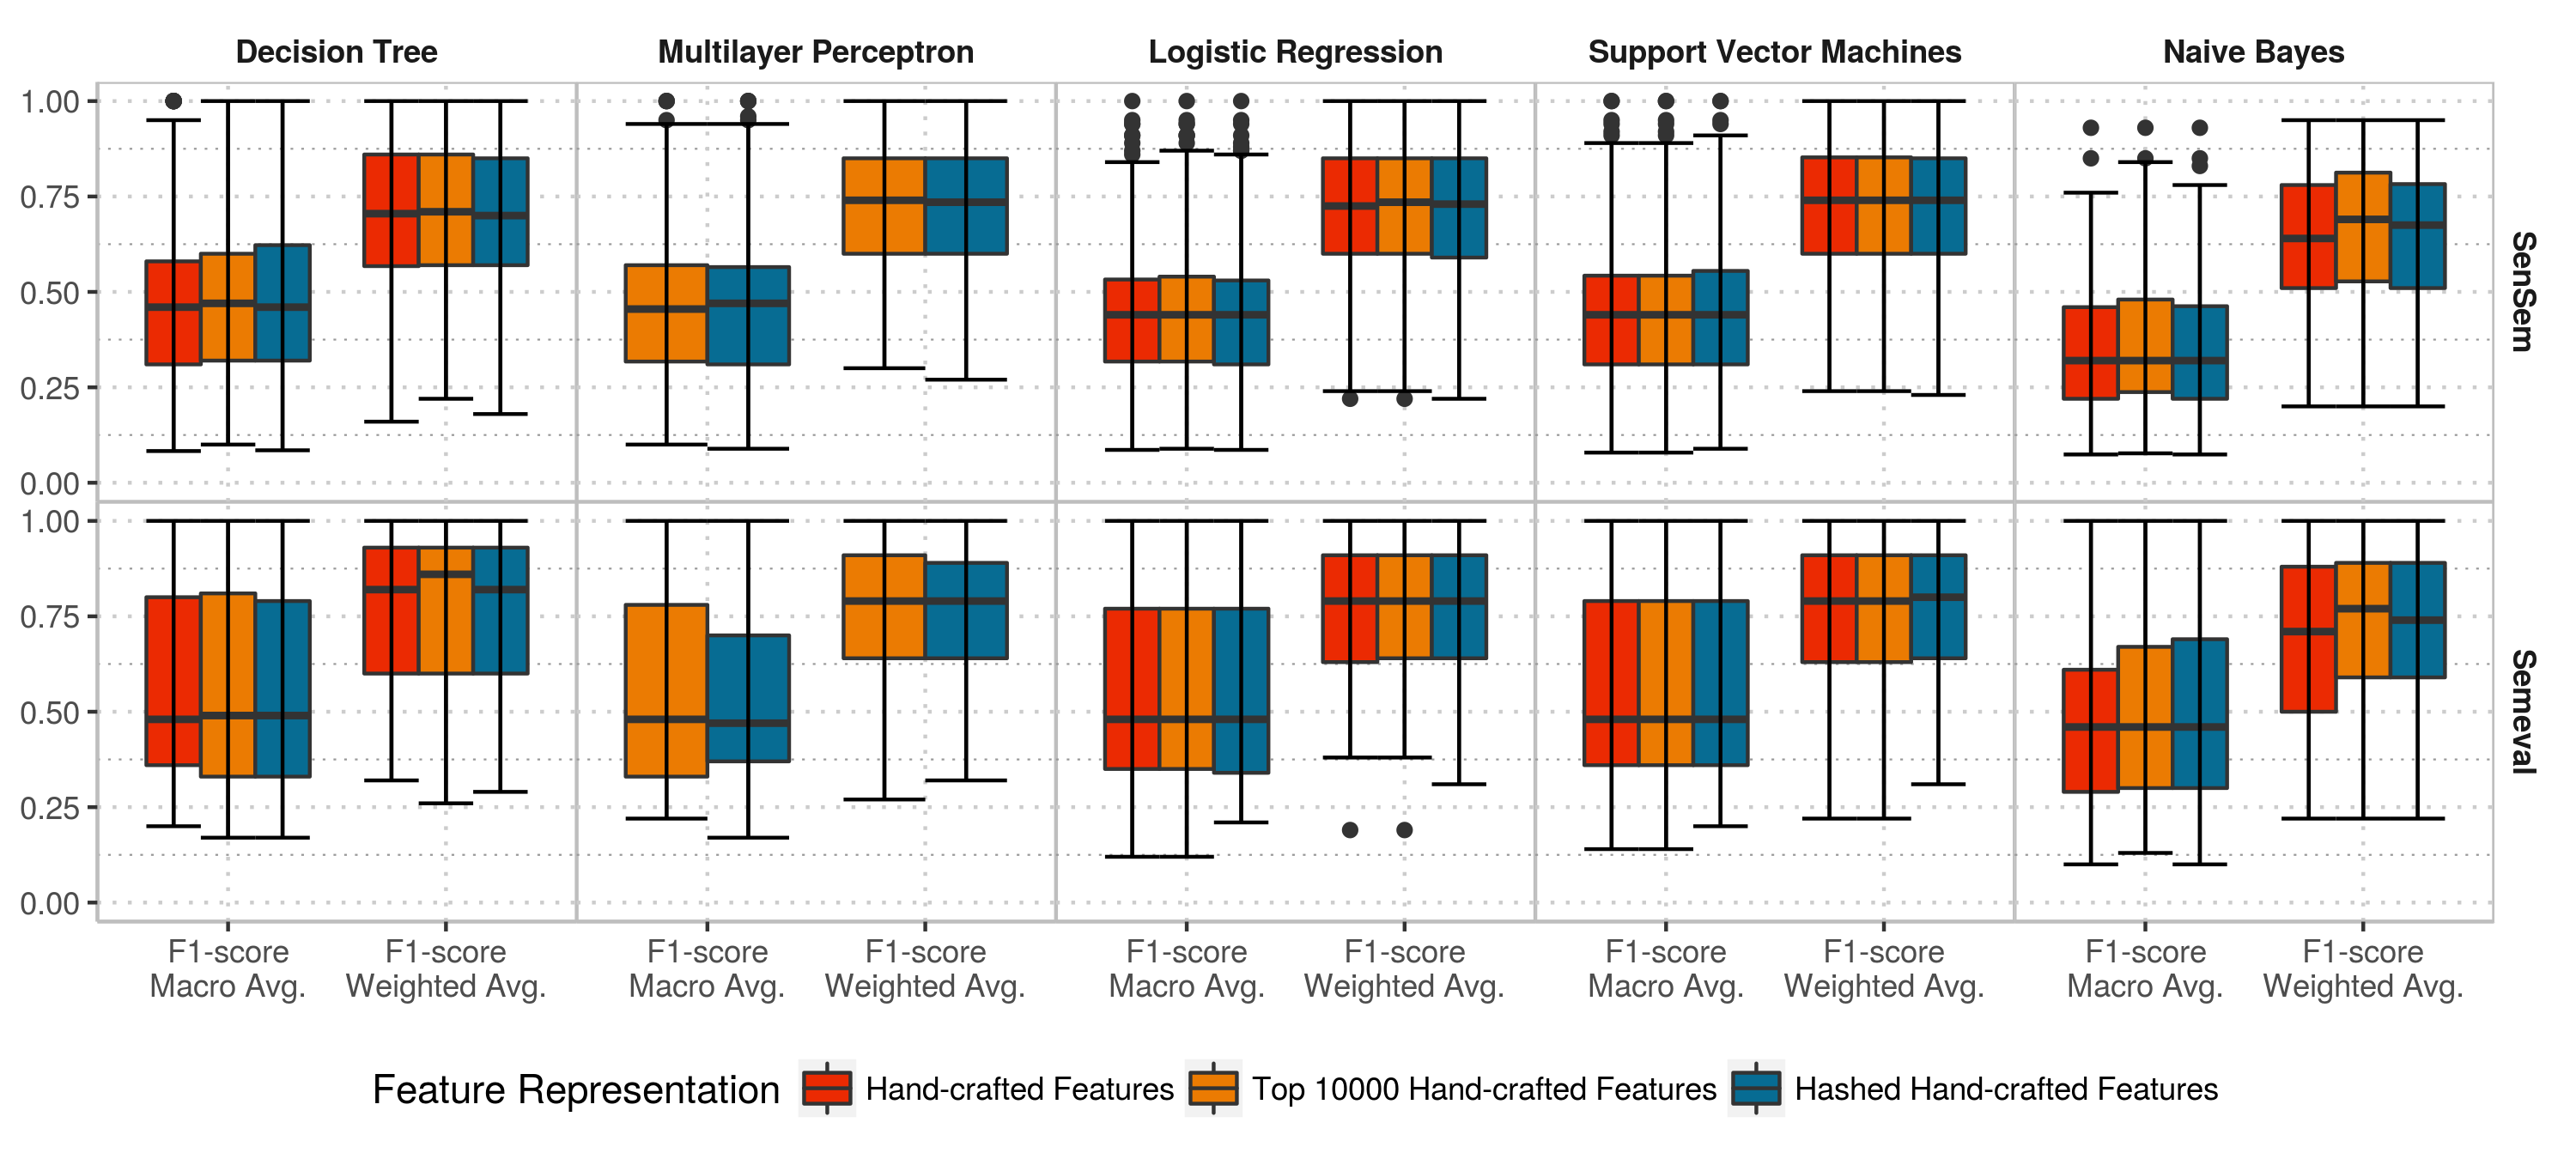
\includegraphics[width=\textwidth]{plots/supervised/representation_comparison}
  \caption{Comparison of feature representations for different classifiers
  using F1-score macro and weighted average}
  \label{fig:supervised:representations}
\end{figure}

Figure \ref{fig:supervised:representations} showcases the different results
of the different models changing the features representation using a box and
whiskers plot. The plot is structured in the following way: 

\begin{itemize}
  \item Each row shows the results for a corpus: SenSem and SemEval.
  \item Each column represents a classifier: decision tree, multilayer
    perceptron (with two hidden layers one of 250 neurons and the other with
    100 neurons), naive Bayes, logistic regression, and support vector
    machines.
  \item Each group of box-plots in each plot represents a metric: F1-score
    macro average and F1-score weighted average.
  \item Each box-plot of different color inside a group is the type of
    representation: all the features, top 10 thousand features selected by the
    feature selection method, and hashed features.
  \item The box and whiskers plots represent the distribution of the values of
    the metrics through their quartiles. Each value is the performance for a
    lemma of the corpus. The black thick line in the middle of a box-plot
    represents the median and the whiskers at the end of each box-plot
    represents maximum and minimum value (except for eventual outliers
    represented by black dots outside the box-plot).
\end{itemize}

First thing to notice in the Figure is the absence of a representation box-plot
in the column corresponding to the multilayer perceptron. This is because of
what was said in the previous paragraph, about a multilayer perceptron being
unable to handle all possible features.

From the graphic I can figure out that there is no distinctive difference from
one representation to the other. In general terms the quartiles are similar,
and the performance depends more on the classifier than the representation. It
is true however that in many (if not all) cases there is a minimal improvement
on the performance by using dimensionality reduction, probably because it makes
the classifiers overfit less when the noise of rare features is removed.
Although it is also true that the use of a feature selection technique has a
little more performance (though still minimal) than the hashing trick, there
was also a trade off because of the computational cost of doing feature
selection for the classification task, which in future experiments using
semi-supervised techniques would become a heavier problem as the number of new
features grows at high pace.

For these reasons, {\em the rest of the experiments were carried out using the
hashing trick representation} as it shows no great drop in performance over the
test set and it is also the cheapest to work with in computational terms.

\subsection{Classifier selection}

In the following chapters I will focus on working with the multilayer
perceptron classifiers. This, again, is to have a point of comparison
particularly in Chapter \ref{chapter:ladder} as Ladder Networks are based on a
multilayer perceptron classifier. It is however important to compare the
multilayer perceptron against other classification methods in order to rule out
the possibility of it being a bad choice to work with from the start.

\subsubsection{Architecture selection}\label{sec:supervised:architecture:selection}

One of the main hyperparameters for a neural network is the architecture.  In a
multilayer perceptron this is the selection of the number of layers and size of
each layer (i.e. number of neurons). As the amount of data is small, there is a
high risk of the network memorizing the datasets. With enough neurons
available, each instance can be mapped to a path in the network.  Thus I cannot
work with a very deep neural network without falling into this problem. That is
why I only look up to three hidden layers.

\begin{figure}[ht]
	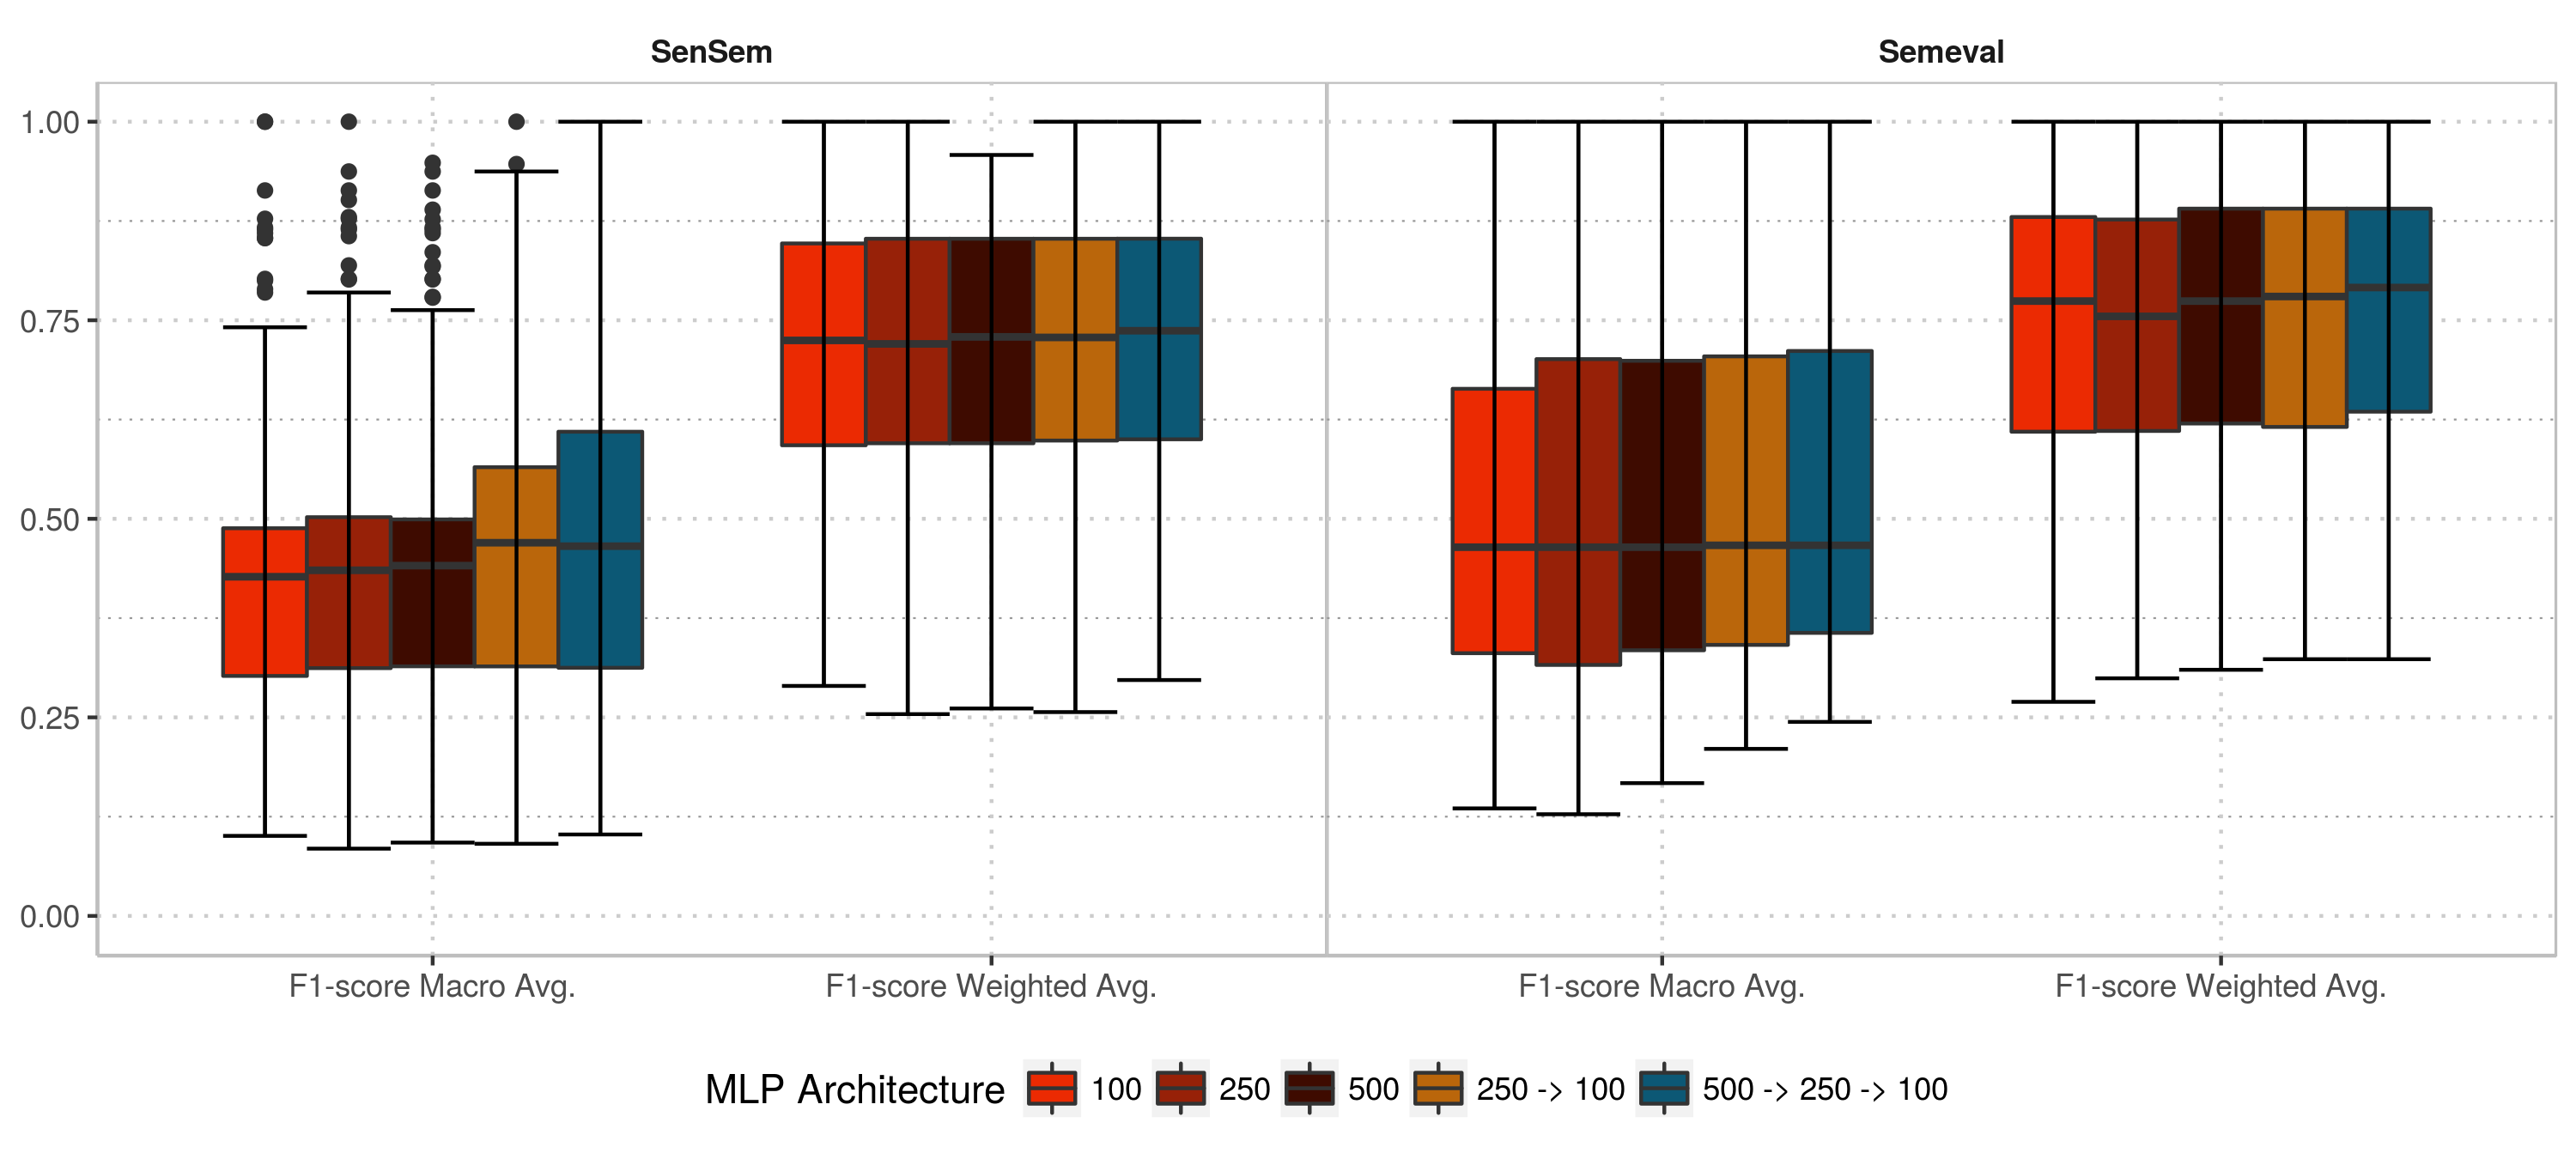
\includegraphics[width=\textwidth]{plots/supervised/mlp_comparison}
  \caption{Comparison of multilayer perceptron architectures}
  \label{fig:supervised:mlp}
\end{figure}

Figure \ref{fig:supervised:mlp} compares different architectures
for a multilayer perceptron using the hashing trick representations (as it was
selected before). This is done only for the following architectures:

\begin{enumerate}
  \item A hidden layer with 100 neurons.
  \item A hidden layer with 250 neurons.
  \item A hidden layer with 500 neurons.
  \item Two hidden layers: the first with 250 neurons, and the second with 100
    neurons.
  \item Three hidden layers: the first with 500 neurons, the second with 250
    neurons, and the third with 100 neurons.
\end{enumerate}

The Figure has a similar structure to that of Figure
\ref{fig:supervised:representations} as it is also a box and whiskers plot
to showcase the performance of each lemma:

\begin{itemize}
  \item Each column represents the corpus: SenSem and SemEval.
  \item The group of box-plots represents the metric: F1-score macro average
    and F1-score weighted average.
  \item Each box-plot of different color represents an architecture of the
    network as described before.
  \item The box and whiskers plots represent the distribution of the
    performance for each lemma as described for Figure
    \ref{fig:supervised:representations}.
\end{itemize}

In this case I can see that the number of neurons does not affect the result
but the number of layers does. The three layer architecture shows the best
results avoiding a high tendency to overfit. There were some other experiments
adding more layers but the improvement on the results was not much more than
with a three layer architecture and, as the number of hyperparameters grow, the
networks were more prone to overfit the data by memorizing it. Plus, the
training time became considerably higher for deeper architectures.

\subsubsection{Comparison of
classifiers}\label{sec:supervised:classifier:comparison}

Figure \ref{fig:supervised:classifiers} showcases the comparison of the
classifiers described in Section \ref{sec:supervised:classifiers}, with an
addition of a baseline classifier which assigns the most frequent sense to every
instance. 

\begin{figure}[ht]
	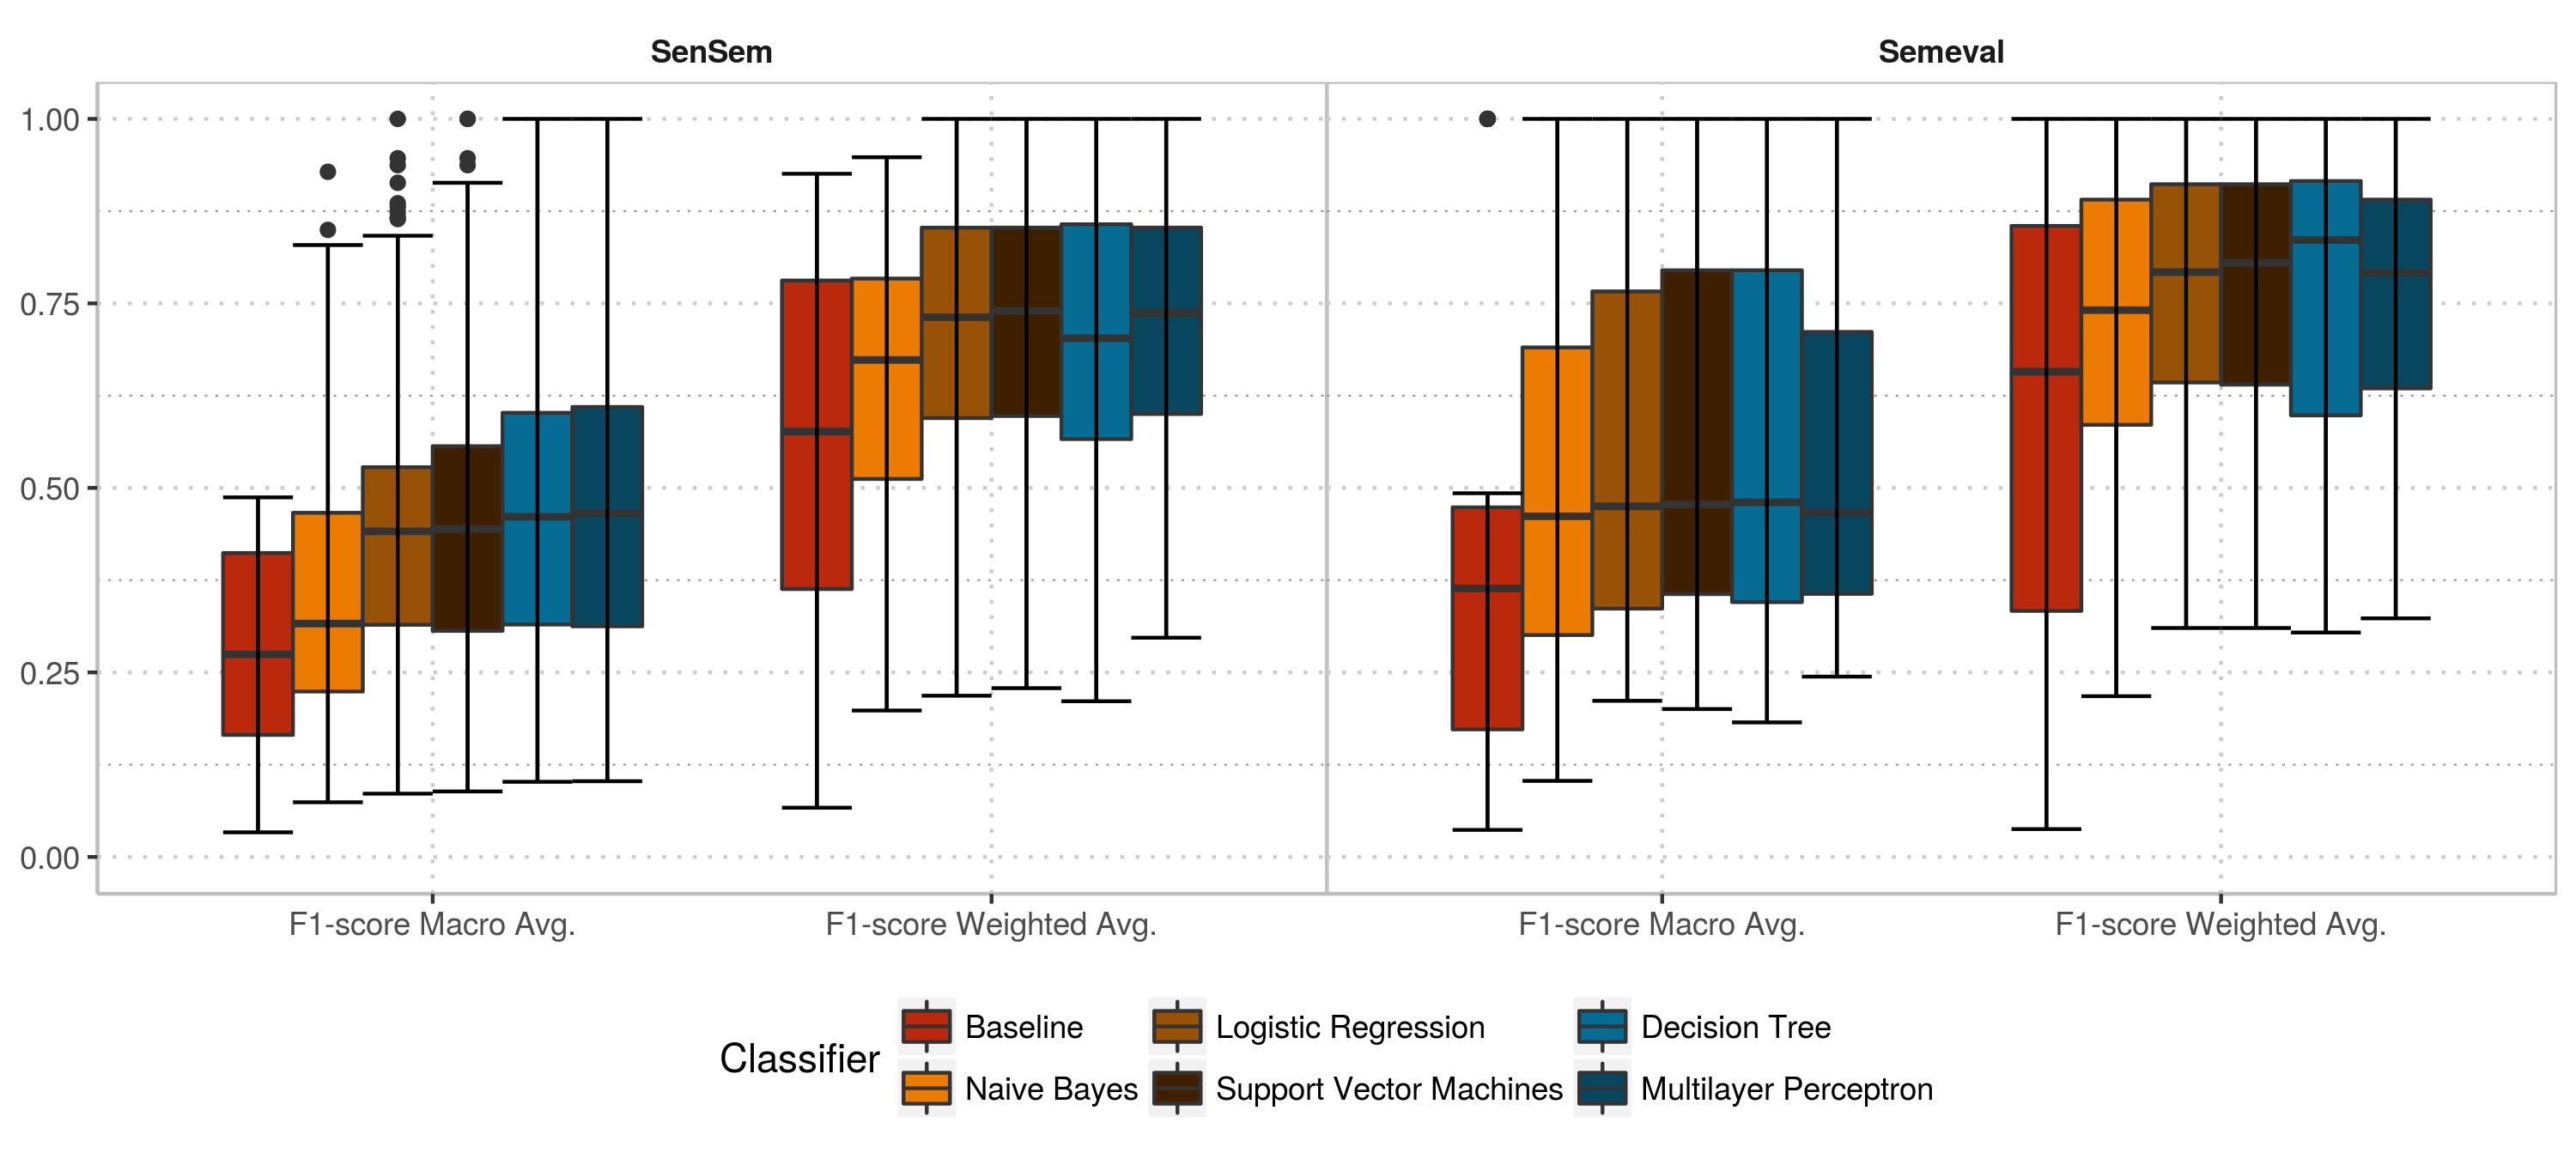
\includegraphics[width=\textwidth]{plots/supervised/classifier_comparison}
  \caption{Comparison of classifiers}
  \label{fig:supervised:classifiers}
\end{figure}

Since it was established that the supervised representation to use in the rest
of the experiments of this thesis is using the hashing trick, the comparison
here is only for such representation. The Figure also has a box and whiskers
plot with a similar structure to that previously shown:

\begin{itemize}
  \item Each column shows the results for a corpus: SenSem and SemEval.
  \item Each group of box-plots represents a metric: F1-score macro average and
    F1-score weighted average.
  \item Each box of different colors inside a group is the classifier:
    baseline, decision tree, multilayer perceptron, naive Bayes, logistic
    regression, and support vector machines.
  \item The box and whiskers plots follows what is described previously
    for Figure \ref{fig:supervised:representations}.
\end{itemize}

First thing to strike out from the plot is that all the classifiers outperform
the baseline classifier described above. In particular, naive Bayes is the one
to show the worst results among the other classifiers, very near to the
performance of the baseline classifier, clearly biased by the most frequent
sense. On the other hand, the decision tree classifier as well as the
multilayer perceptron classifier (with the architecture defined in the previous
section) show the best performances for SenSem corpus if we focus in minority
classes. However, in a weighted average the decision tree has a worse
performance than SVM, LR or MLP.

For SemEval there is less disparity between the performance of the classifiers
(still being naive Bayes the one with worse performance, besides the baseline),
with the median being similar for all of them, and being the decision tree the
one having the best performance in a weighted average. 

Seeing that decision trees and multilayer perceptrons are the ones with the
best performances, there is a strong indication that the problem of
\vsd~is non-linear.

\subsubsection{Significance}

The previous results are good enough to assert that a multilayer perceptron is
a good approach to model the problem of \vsd. However, in order to see whether
the difference in performance is significant or not, I should test it using
Metric \ref{met:2} and seeing the Cohen's kappa coefficient between the
different classifiers.

\begin{figure}[ht]
	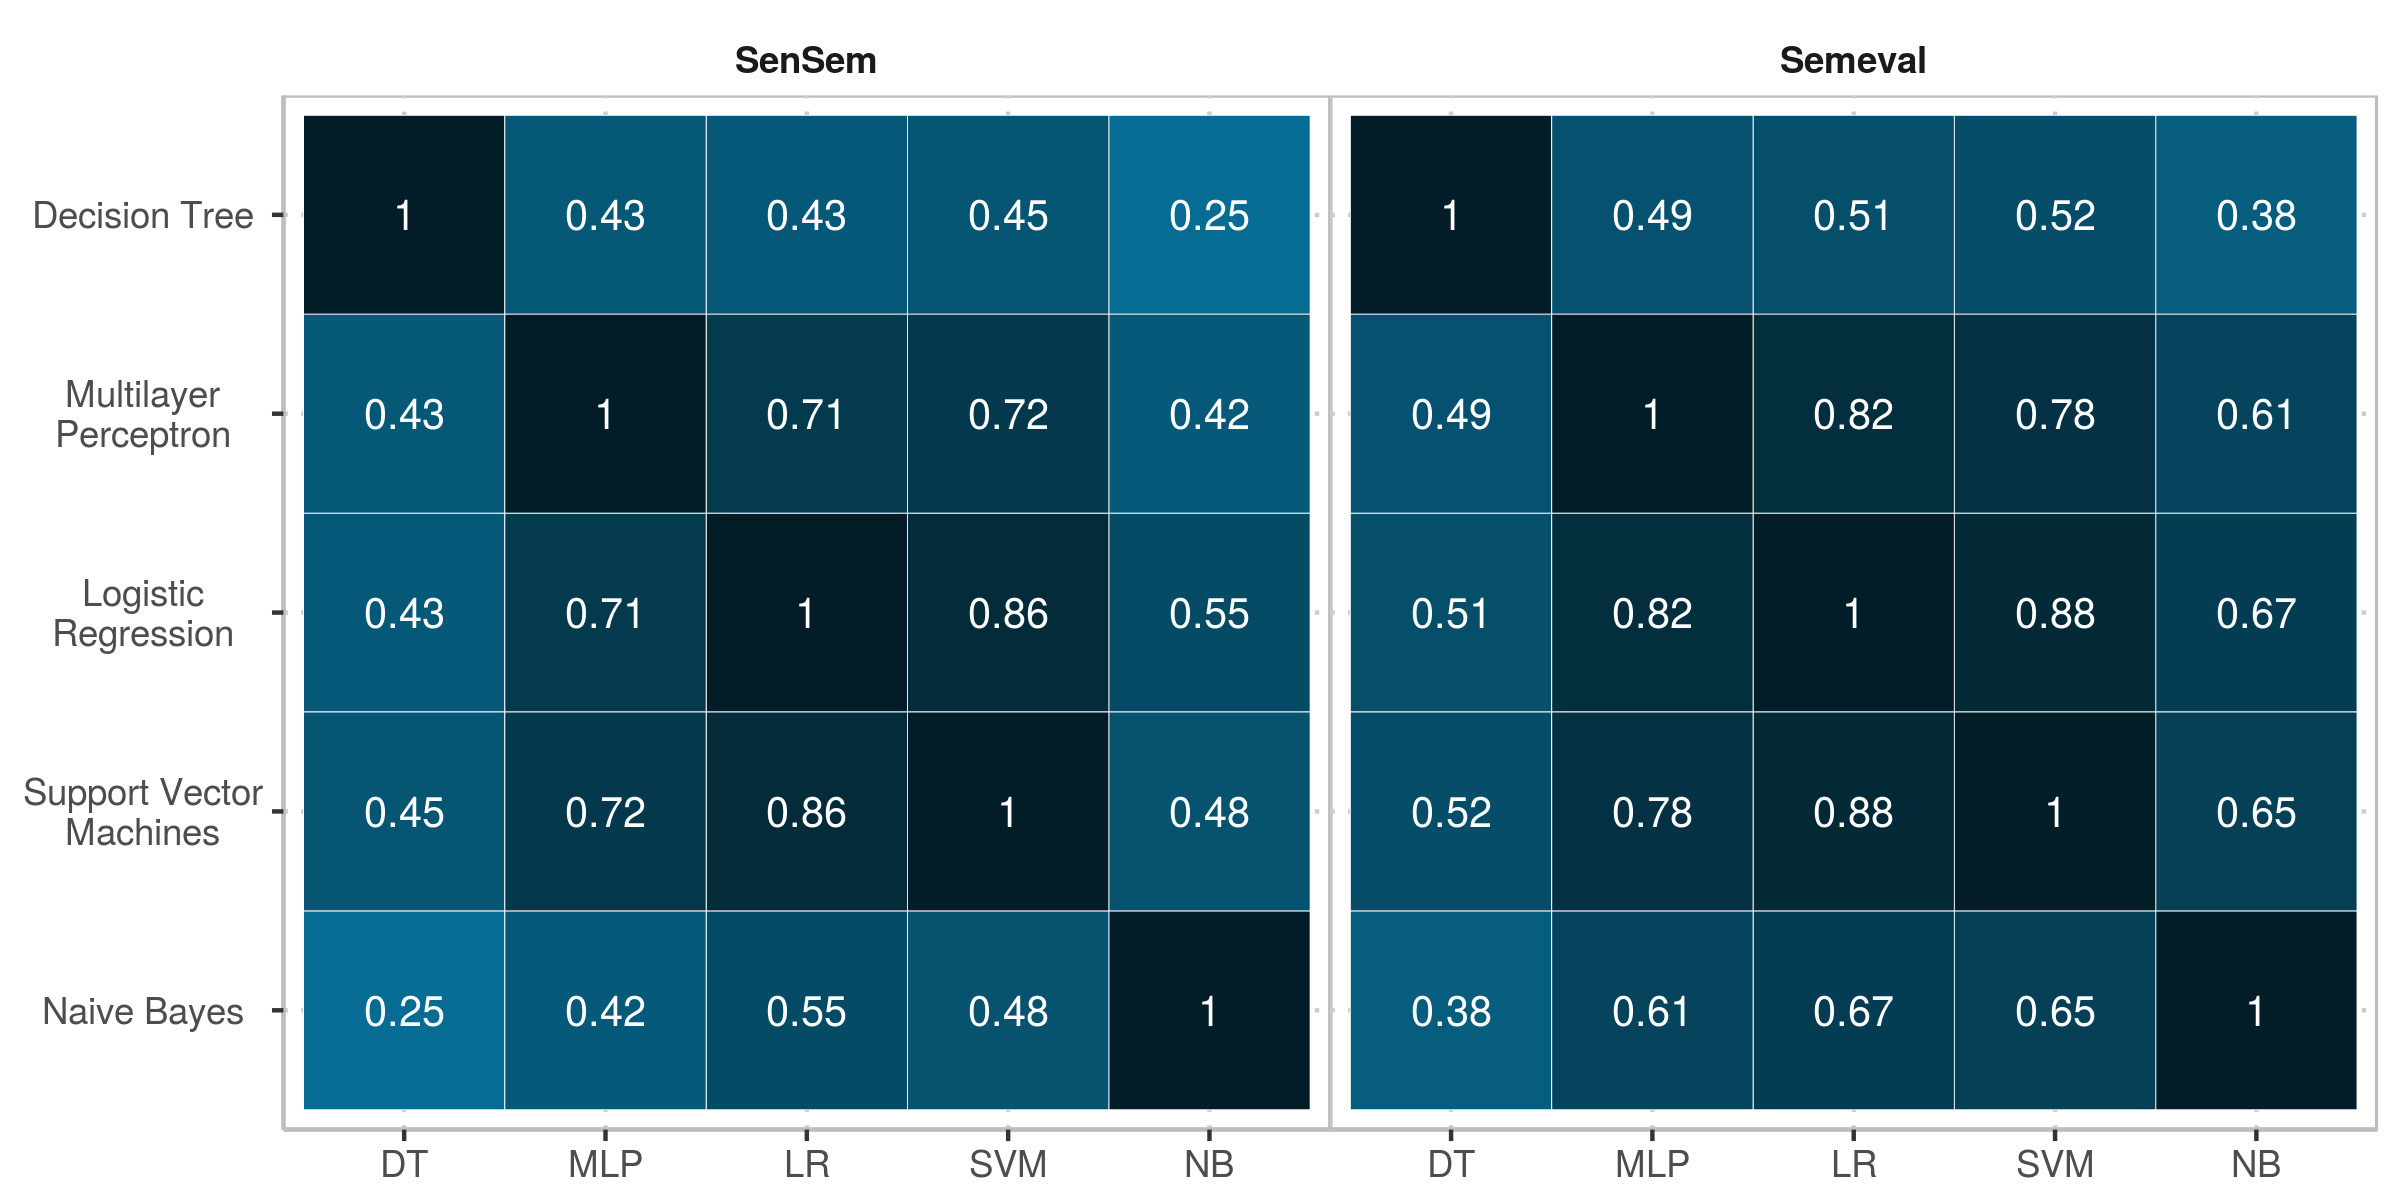
\includegraphics[width=\textwidth]{plots/supervised/inteclassifier_kappa}
  \caption{Cohen's kappa coefficient between classifiers}
  \label{fig:supervised:kappa}
\end{figure}

Figure \ref{fig:supervised:kappa} shows with a heatmap the mean of the Cohen's
kappa coefficient between the classification results of each classifier per
lemma over the test corpus. The higher the kappa, the more similar the
classification, thus the less significant the difference between classifiers.
The color of the heatmap defines the value for inter-classifier kappa between
the classifier of the row and the classifier of the column. The heatmap is
symmetric.

The logistic regression and SVM classifiers are the ones having the most
agreement, probably because they are both linear classifiers. Thus the
difference in performance between them is not really significant. The
multilayer perceptron is the most similar to these two. Decision trees and
naive Bayes are the ones to show the less agreement compared to the other
classifiers. Naive Bayes is likely to have a low agreement as it is one of the
classifiers with worse performance. Although it is not trivial to set a
threshold for which the kappa statistic is good to denote statistical
significance, I can infer from this plot that decision tree learning is clearly
having good performance with statistically significant difference with other
classifiers that are also performing well, which makes it more interesting to
continue exploring in future work. 

\subsection{Hypothesis \ref{hyp:supervised:1}}\label{sec:supervised:hyp:1}

Once the base model to work with for the following experiments is selected, I
can start testing the hypotheses set in Section \ref{sec:supervised:overview}.

I start by looking at the results to test Hypothesis \ref{hyp:supervised:1}.
Recall the hypothesis states that larger training datasets help improving the
performance. To check the validity of this I follow the steps of Experiment
\ref{exp:supervised:2}. I use the multilayer perceptron with three layers
I selected in previous paragraphs.

\begin{figure}[ht]
	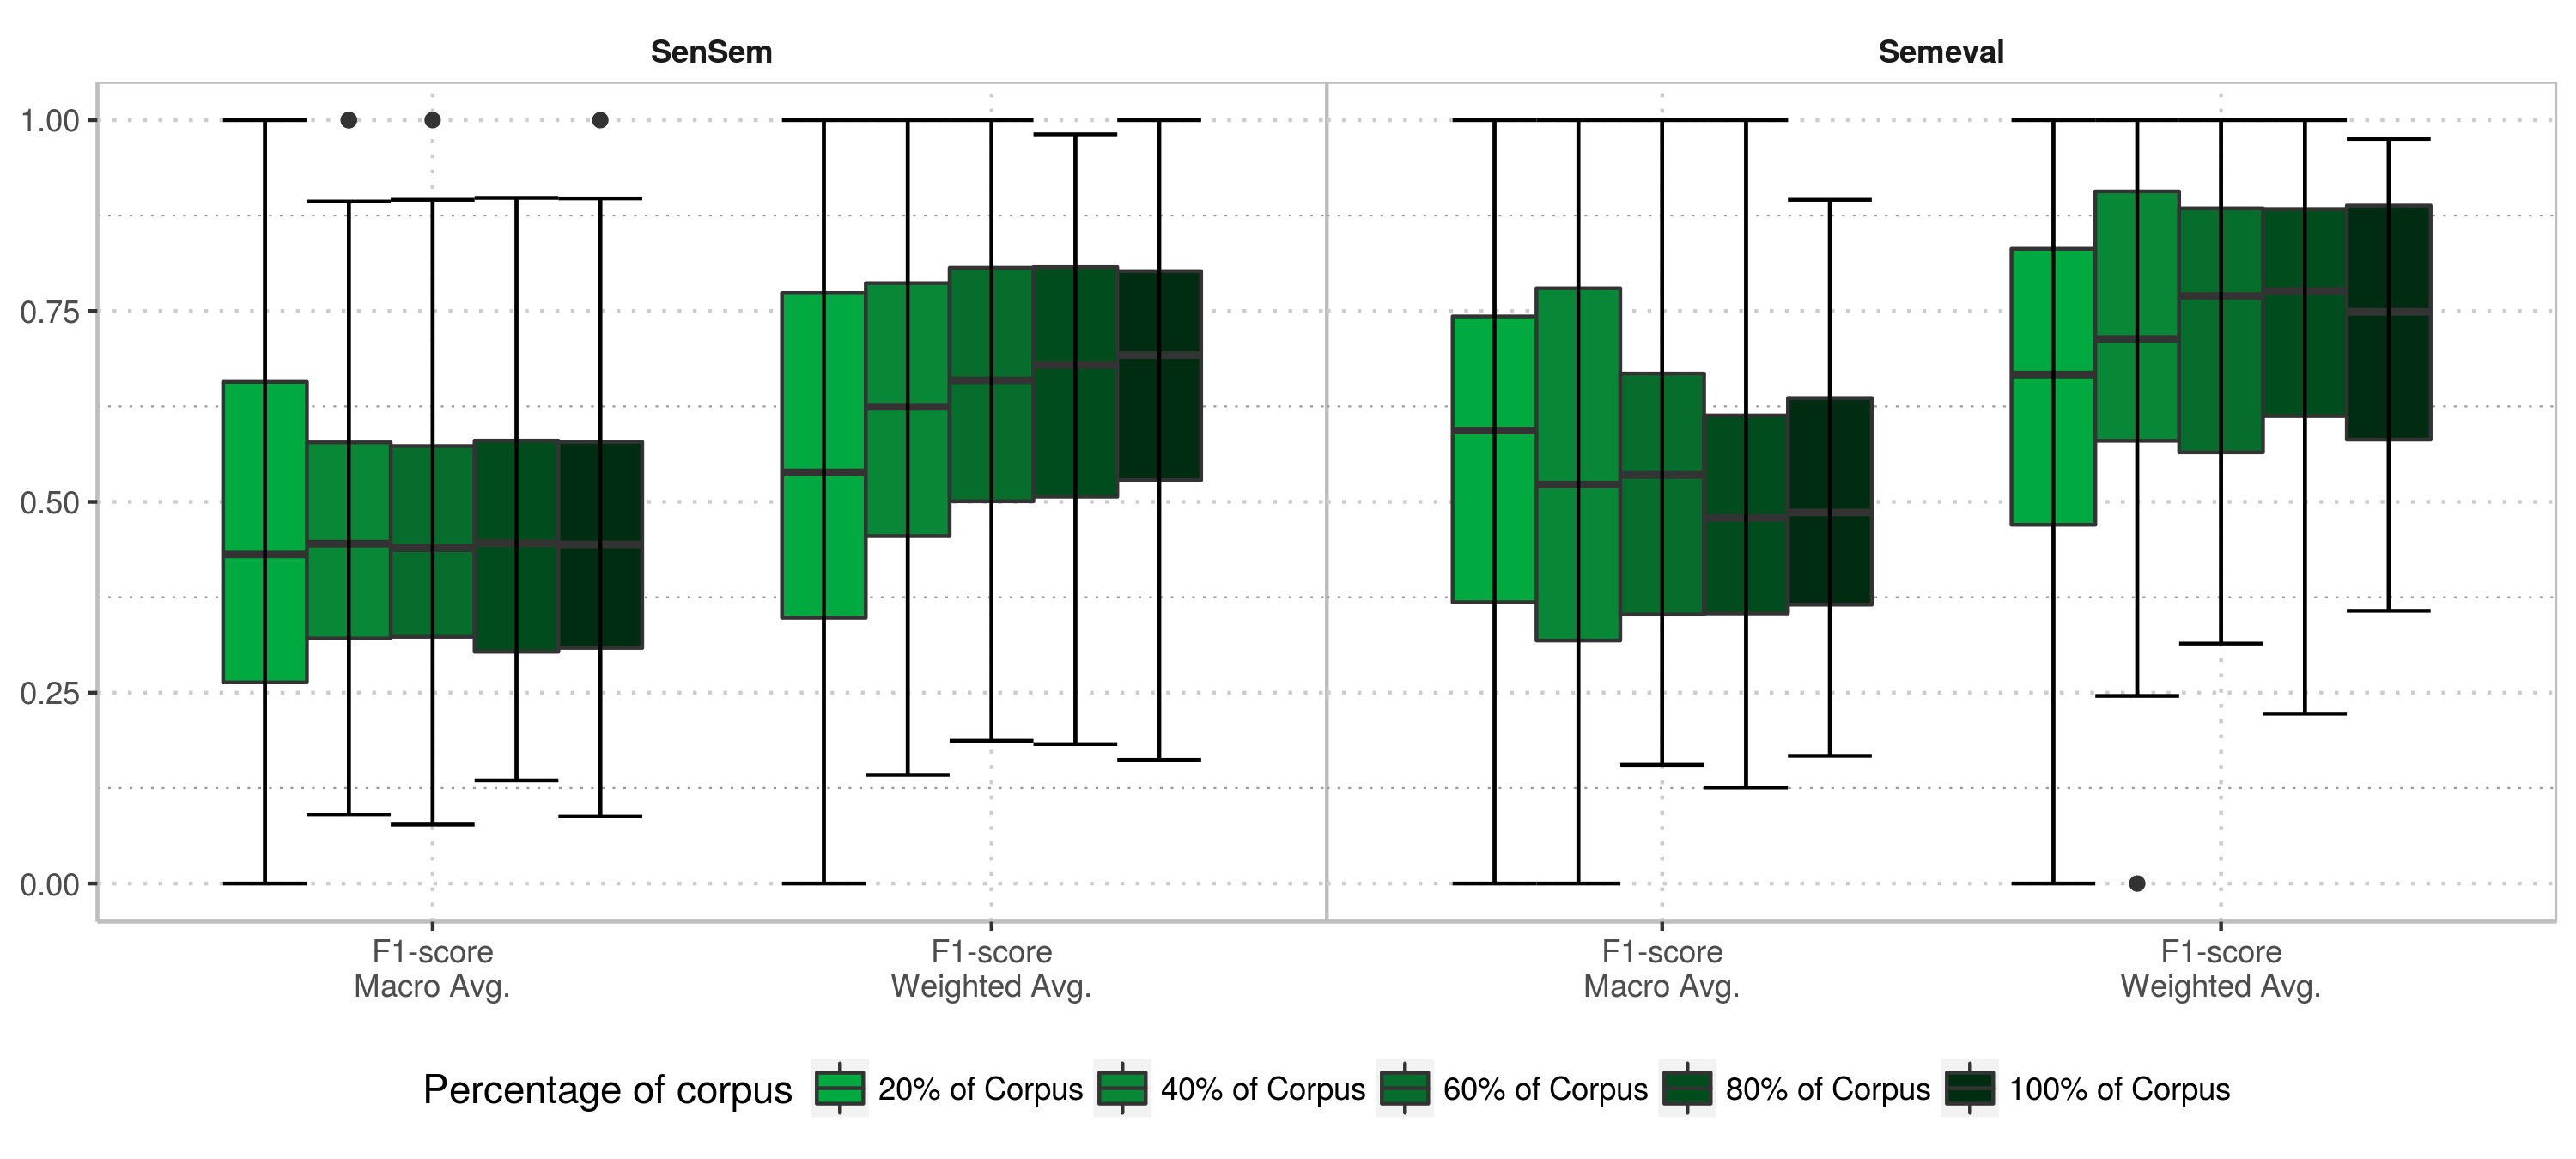
\includegraphics[width=\textwidth]{plots/supervised/performance_progress}
  \caption{Performance per lemma on the test corpus for different sizes of
  training corpus}
  \label{fig:supervised:performance_progression}
\end{figure}

Figure \ref{fig:supervised:performance_progression} shows the performance on
the test corpus for different sizes of the training corpus (as a percentage of
the full training corpus). The figure shows a box and whiskers plot following 
a similar structure shown before:

\begin{itemize}
  \item Each column shows the results for a corpus: SenSem and SemEval.
  \item Each group of box-plots shows the different metrics: F1-score macro
    and weighted average.
  \item Each box-plot of a different shade of color shows the performance for
    different sizes of the training set (as percentage of the total training
    data).
  \item Each box and whiskers plot follows what is described previously for
    Figure \ref{fig:supervised:representations}.
\end{itemize}

The first thing to note from this figure is how, increasing the number of
examples does not necessarily improve the performance of the classifier. This
is due to the fact that in the process to progressively enlarge the corpus
examples are added aiming to have each class represented. When the corpus is
very small, minority classes are comparatively well represented. But as the
number of examples increases, the imbalance between classes also increases.
This results in no performance gain (SenSem) or even degradation of the
performance (SemEval)for minority classes, as can be well seen in the macro
average metric. The weighted average improves with the number of examples in
the case of SenSem, which is a very small corpus, but not so much in the case
of SemEval, which is much bigger. Thus increasing the number of examples seems
good to improve a small corpus but not necessarily a bigger corpus. The main
reason for this seems to be the problem of class imbalance, that becomes more
and more acute as the number
of examples increases.

This however is difficult to see clearly, as the box-plots are useful for
giving a general idea of the performance for many different models, but they
obscure the particular performance of a specific model. As I have one model per
lemma, I would need to examine more closely 200 hundred different models to see
how it is working for each lemma, something outside the scope of this thesis.

There is a clear pattern nevertheless in how a model improves performance with
more training data, specially in cases of models with extremely low
performance: there are models that initially have an F1-score of 0 for the
models trained with the less data, something that does not happen with more
added data.

\subsection{Hypothesis \ref{hyp:supervised:2}}\label{sec:supervised:hyp:2}

To check Hypothesis \ref{hyp:supervised:2} I recall that I would do so
with aid of Experiment \ref{exp:supervised:3}. The hypothesis states
that the size of the dataset not only affects the performance (measured by
Metric \ref{met:1}), but also the tendency to overfit (measured
by Metric \ref{met:3}) of a model.

\begin{figure}[ht]
	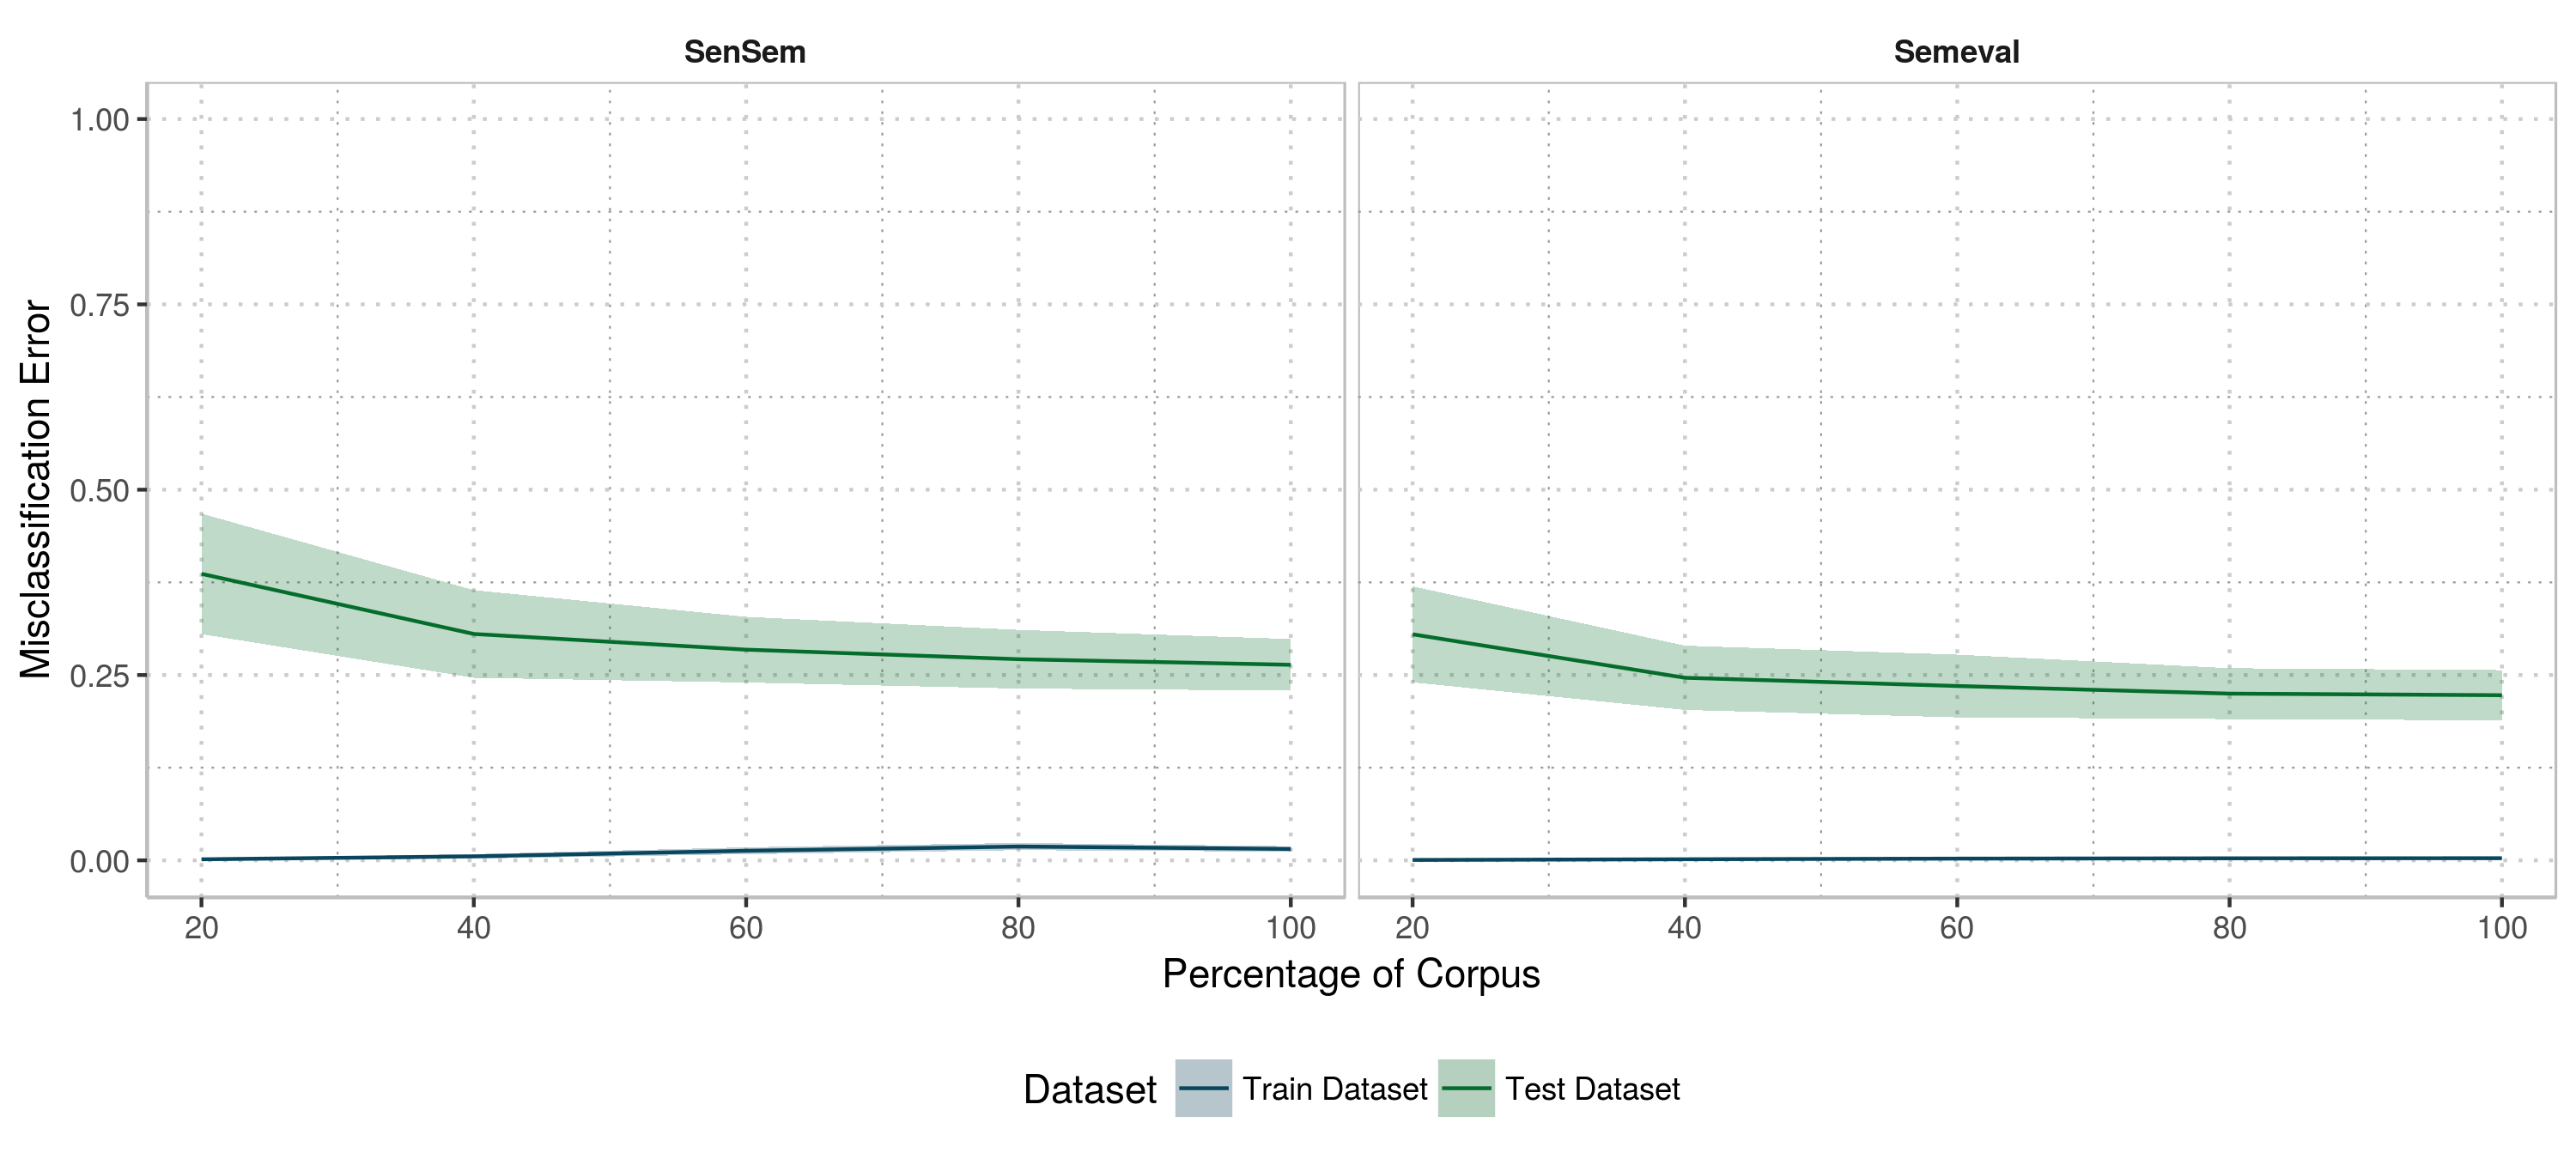
\includegraphics[width=\textwidth]{plots/supervised/learning_curve_scores}
  \caption{Learning curve for different sizes of training corpus}
  \label{fig:supervised:learning_curve}
\end{figure}

Figure \ref{fig:supervised:learning_curve} shows the learning curve for
different sizes of the training data. The structure of the learning curve plot
is as follows:

\begin{itemize}
  \item The plot is divided in two columns, each represents a corpus: SenSem
    and SemEval.
  \item The x-coordinate shows the size of the training data, as a percentage
    of the total training data available, starting from 20\% of the corpus (the
    corpus was split in 5 parts according to Experiment
    \ref{exp:supervised:3}).
  \item The y-coordinate shows the misclassification error of a model.
  \item There are two colors representing the datasets: train and test.
  \item The solid darker lines represent the mean of misclassification error
    trough the different splits of the datasets over all the models.
  \item The shadowed area, which have a lighter color, represent the standard
    error of the mean of the misclassification error.
\end{itemize}

Recall Experiment \ref{exp:supervised:3} first split the corpora in uniform
size parts and gradually added those new parts to the training and evaluation
of the model. It trained a model on a portion and evaluated it on the other,
held-out, portion and recorded the results. It repeated the algorithm a number
of times over different ways of splitting the data to see how the same model
behaves on different datasets. Figure \ref{fig:supervised:learning_curve}
shows the mean and standard error of the mean over the misclassification error
each model has in the training and test datasets.

The test data is having a visible variance of the misclassification error, seen
in the wide shadowed area, while the training data is having almost no
misclassification error, as the shadowed area is indistinguishable of the line
representing the mean of the misclassification error.

In the plot there are two indicators of an error due to variance:

\begin{itemize}
  \item A wider shadowed area: means that the misclassification error of
    different models has a high variance, thus making the models more
    inconsistent over different datasets.
  \item A higher mean of the misclassification error of the test set in
    comparison to the mean training set error, means the model is overfitting
    to the training data.
\end{itemize}

As I clearly see in Figure \ref{fig:supervised:learning_curve}, this variance
is smaller the more training data I have. This is a strong indication of
Hypothesis \ref{hyp:supervised:2} being true, as there is less overfitting in
the different models the more data is used for training.

\subsection{Hypothesis \ref{hyp:supervised:3}}\label{sec:supervised:hyp:3}

To check Hypothesis \ref{hyp:supervised:3} I would do so with aid of
Experiment \ref{exp:supervised:3}. I recall the Hypothesis stated that the
number of classes affects the tendency to overfit (as measured by Metric
\ref{met:3}). To show this I plot the training curve measuring the
mean of lemmas having different number of total labels.

\begin{figure}[ht]
	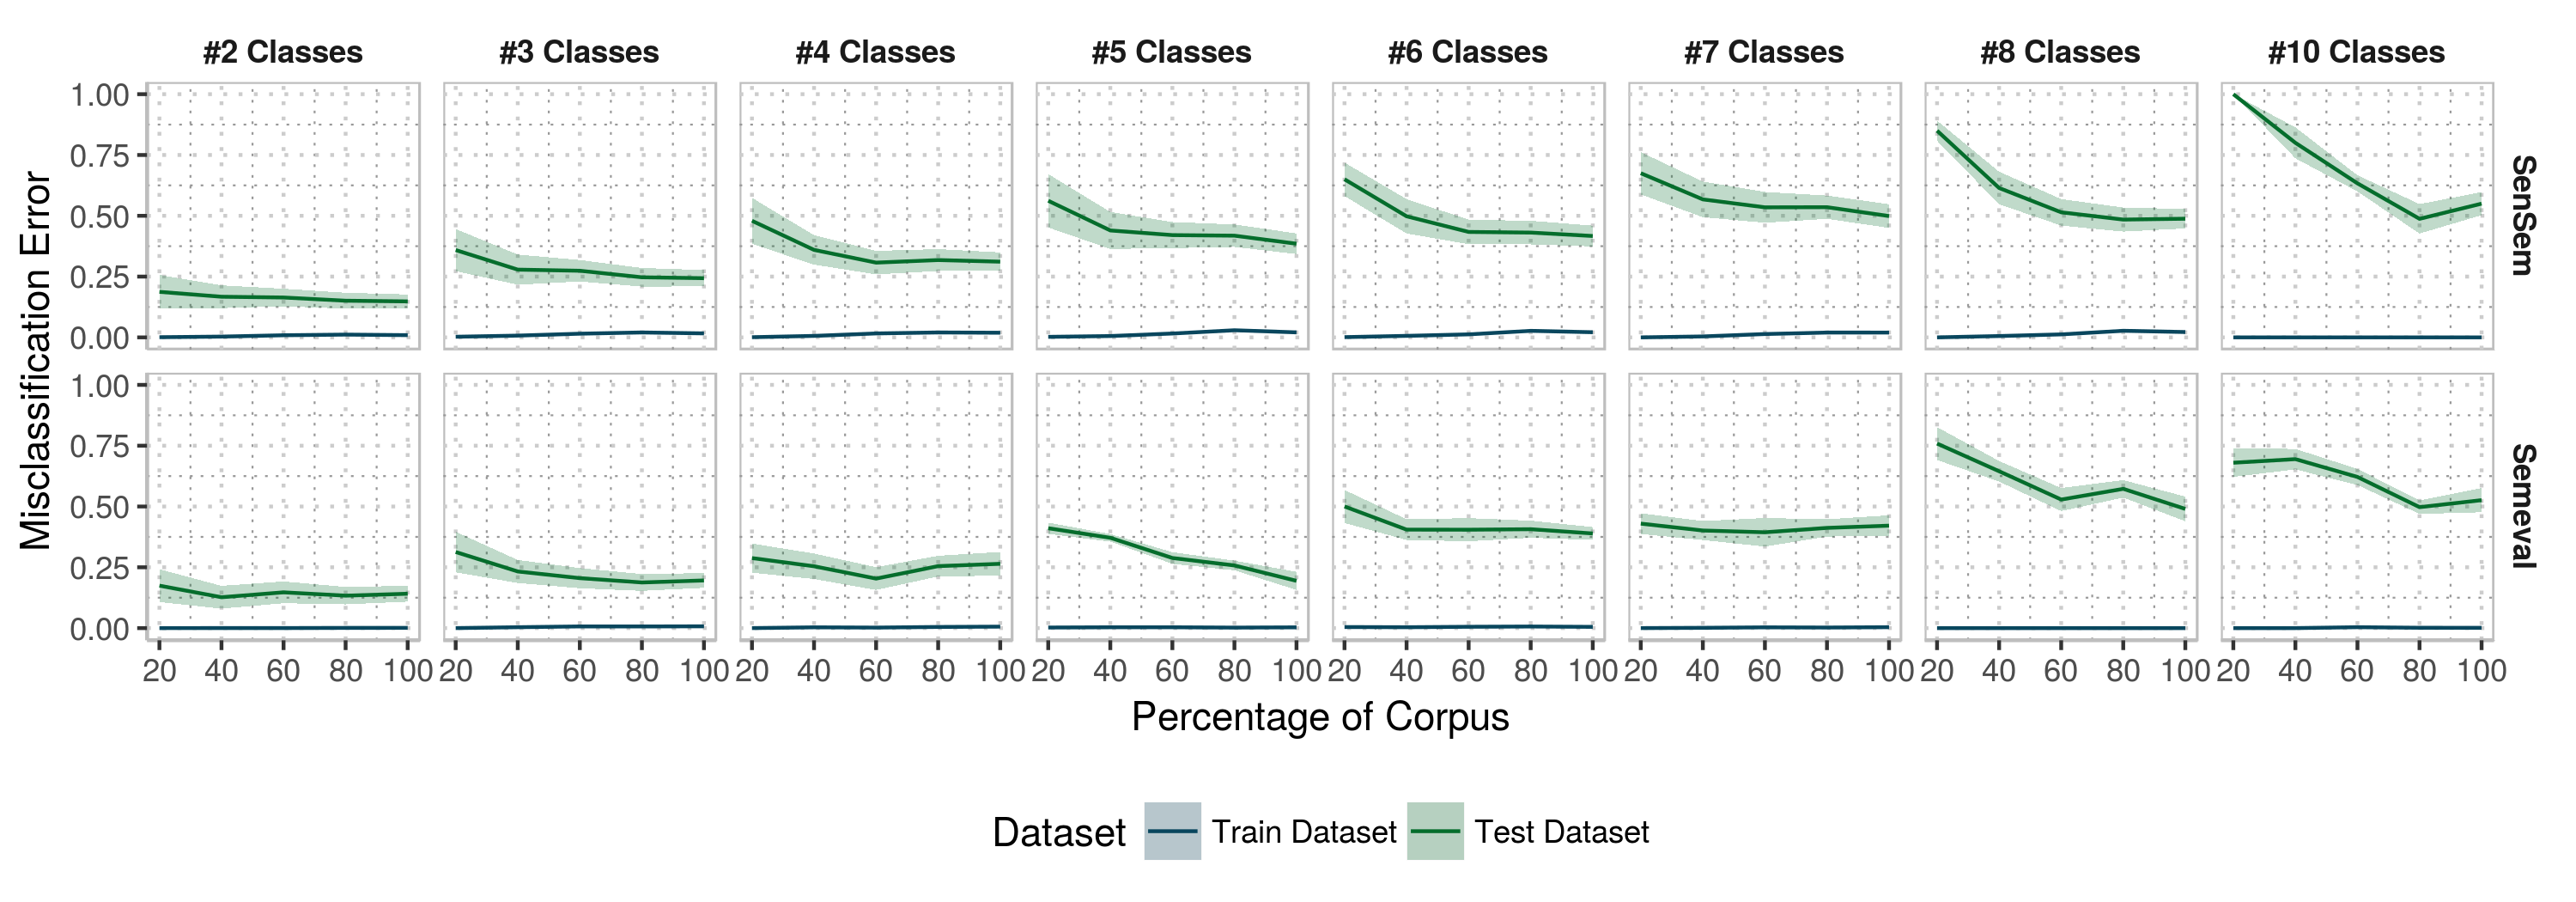
\includegraphics[width=\textwidth]{plots/supervised/learning_curve_per_class_num}
  \caption{Learning curve for different number of classes}
  \label{fig:supervised:learning_curve_per_class_num}
\end{figure}

Figure \ref{fig:supervised:learning_curve_per_class_num} shows the learning
curve for different number of classes. The structure of the plot is similar to
Figure \ref{fig:supervised:learning_curve} with some minor changes to showcase
what the Hypothesis states:

\begin{itemize}
  \item The plot is divided in two rows, each represents a corpus: SenSem and
    SemEval.
  \item The columns of the plots represent the number of classes of the
    models: 2, 3, 4, 5, 6, 7, 8, and 10 classes.
  \item The x-coordinate is the size of the training data as explained in
    Section \ref{sec:supervised:hyp:2}.
  \item The y-coordinate shows the misclassification error.
  \item The colors, lines and shadowed area represent the same thing described
    in Section \ref{sec:supervised:hyp:2}.
\end{itemize}

The models are one for each lemma, thus Figure
\ref{fig:supervised:learning_curve_per_class_num} shows in each column the mean
of all the models having that number of classes (senses). The pattern of the
Figure is clear, as the mean of the error due to variance is larger the more
classes the model has. The error due to high variance is higher in the models
with more classes as a result of the distribution of the classes, which is
Zipfian. As the tendency to classify all the data as part of the most frequent
class when there is not enough data of the other classes, the misclassification
error of the test data is higher than the training error. These results give
evidences to not reject Hypothesis \ref{hyp:supervised:3}.

\subsection{Hypothesis \ref{hyp:supervised:4}}\label{sec:supervised:hyp:4}

To check Hypothesis \ref{hyp:supervised:4} I use Experiment
\ref{exp:supervised:3}. This Hypothesis states that linear models have less
tendency to overfit that non-linear models. This Hypothesis is looking to
check whether the non-linearity of a model affects its tendency to overfit the
data.

\begin{figure}[ht]
	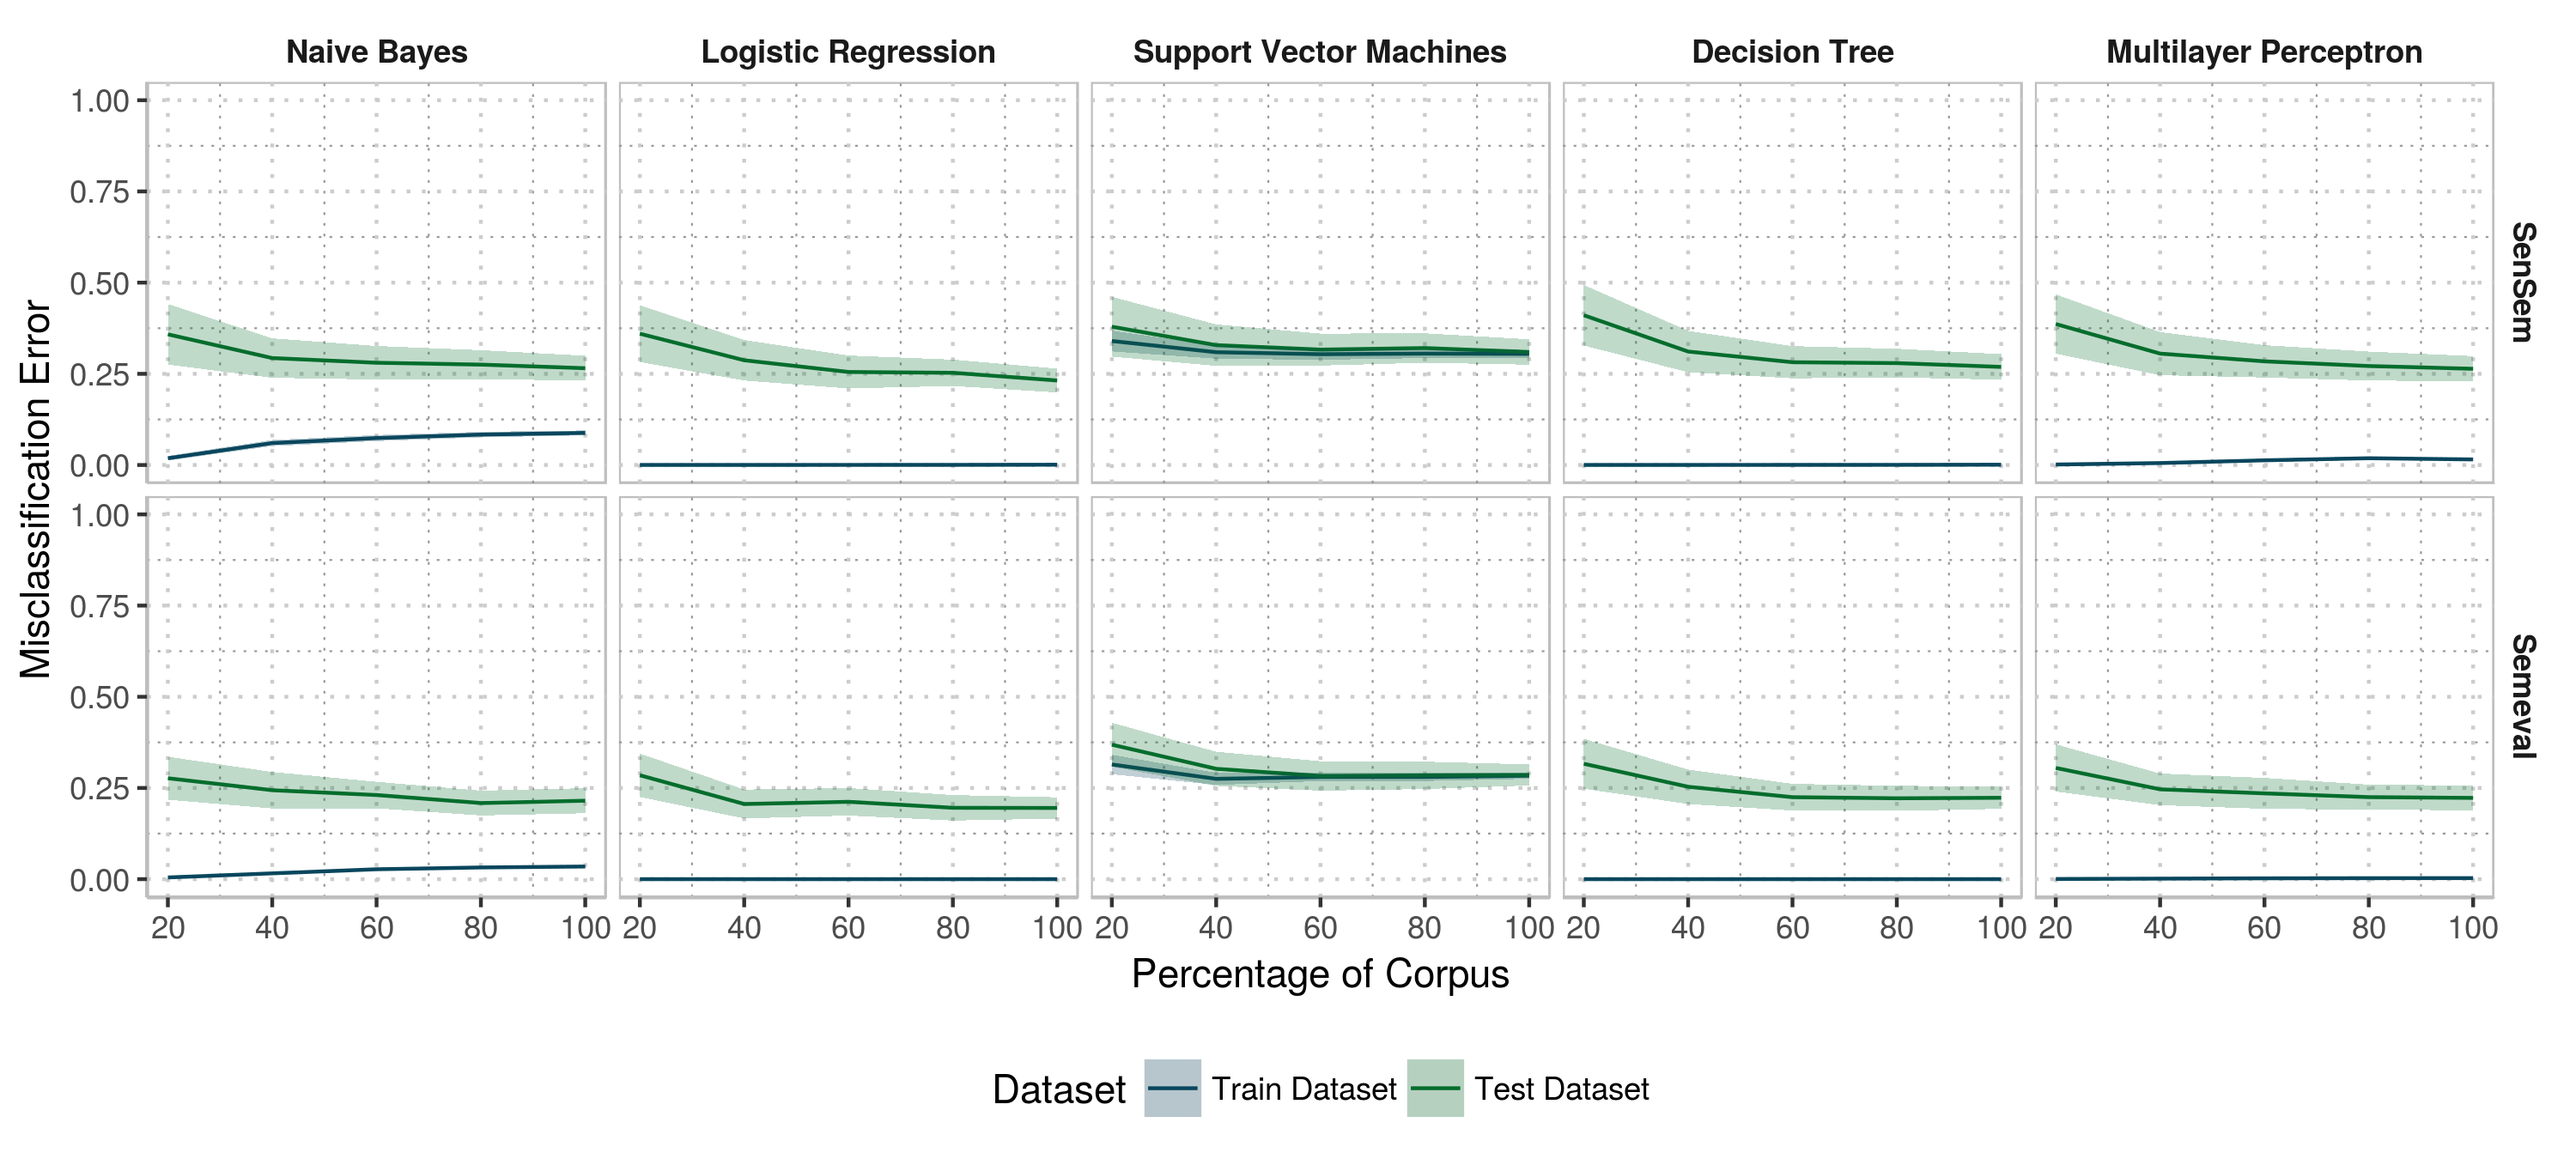
\includegraphics[width=\textwidth]{plots/supervised/learning_curve_per_classifier}
  \caption{Learning curve for different sizes of training corpus per classifier}
  \label{fig:supervised:learning_curve_per_classifier}
\end{figure}

Figure \ref{fig:supervised:learning_curve_per_classifier} showcases the
learning curve for different kind of classifiers (the ones presented in Section
\ref{sec:supervised:classifiers}). The Figure uses a similar structure to that
of Figure \ref{fig:supervised:learning_curve_per_class_num}, but changes what
the columns represent:

\begin{itemize}
  \item The rows of the plot represent the different corpora: SenSem and
    SemEval.
  \item The columns of the plot represent the different classifiers: Naive
    Bayes, Logistic Regression, Support Vector Machines, Decision Tree and
    Multilayer Perceptron. Note that the linear classifiers are the first
    three ones from the left and the non-linear classifier are the last two
    from the left.
  \item The x-coordinate represents the size of the training data as a
    percentage of the total training data.
  \item The colors, lines and shadowed area represent the same thing described
    in Section \ref{sec:supervised:hyp:2}.
\end{itemize}

The first thing that highlight in the plot are the results for Naive Bayes and
Support Vector Machines. In both cases, the training error is not so close to 0
as it is for the other classifiers. 

In Naive Bayes, the error of the training data increases with the number of
training instances. Remember in Section
\ref{sec:supervised:classifier:comparison}, I saw Naive Bayes was the
classifier with the lowest performance and I figure out this was a result of it
being biases towards the most frequent class. Figure
\ref{fig:supervised:learning_curve_per_classifier} gives even more evidence to
support that claim. Naive Bayes then shows less difference between the training
error and the test error as it sacrifices the performance of the model for more
generality of it.

Support Vector Machines shows a wider shadowed area of the training dataset
misclassification error, which means a higher variance of the performance in
the training data. SVM with a linear kernel separates the data with an
hyperplane of maximum margins, just as naive Bayes, it sacrifices good
performance of the training data for a better performance over the general
data.

The other three methods show very similar results, with decision trees being
slightly higher than the rest and logistic regression being slightly lower.
However, from the visual results I see the significance of this difference
in performance is not significant.

The results shown are supportive of Hypothesis \ref{hyp:supervised:4}, as
the linear classifiers show less tendency to overfit, although is at expense
of a higher error due to bias.

\section{Conclusions}\label{sec:supervised:conclusions}

This chapter introduces the problem of \vsd~using purely supervised methods.
The hypothesis I want to test is that the size of the training
set affects the performance of a model. This initial hypothesis was divided
into more specific subhypotheses, which the experimentation and analysis of
results tried to accept or reject.

I designed some experiments to see if there was a significant difference
between different models. A first step was to rule out that techniques to
reduce dimensionality of the representations affected the performance of the
models. This was shown true with the results in Section
\ref{sec:supervised:representation:selection}.

For the neural network classifier, I needed to set the architecture of the
network. The results reported that an architecture with more layers improved
the performance of the model. This was not the case for the number
of neurons per layer. Section \ref{sec:supervised:architecture:selection} shows
these results.

Finally, I compared the performance of the neural network classifier with the
other classifiers defined in Section \ref{sec:supervised:classifiers}. Section
\ref{sec:supervised:classifier:comparison} shows the neural network had one of
the best performances for the SenSem corpus. Nevertheless, the Kappa
coefficient did not report significance in this improvement over the other
classifiers. In any case the objective was to check whether the neural network
was outperformed by other classifiers, which was not the case. The neural
network, as I will show, is the classifier that I finally chose because its
performance was not worse than the others and it is comparable to the
classifiers explored in future chapters.

The experiments done to accept or reject Hypothesis \ref{hyp:supervised:1} that
larger training dataset improve on the performance are observable in Section
\ref{sec:supervised:hyp:1}. The reported results give strong indications about
the validity of the Hypothesis, since there is a visible improvement in the
overall results as the number of training examples increases, thus the
Hypothesis cannot be rejected.

Hypothesis \ref{hyp:supervised:2} cannot be rejected since results of Section
\ref{sec:supervised:hyp:2} give a strong evidence to support it. Indeed,
the tendency to overfit and the error due to variance decrease the more
training data the model has.

In the same way Hypothesis \ref{hyp:supervised:3} cannot be rejected because of
the evidence in results of Section \ref{sec:supervised:hyp:3}. The number of
classes (senses) affects the overfitting of the model. The more classes, the
more difficult for the model not to overfit.

Finally, experiments to test Hypothesis \ref{hyp:supervised:4}, which expects
linear models to have less tendency to overfit than non-linear models, do not
yield conclusive results, although in a shallow observation the results can be
interpreted in favor of not rejecting the Hypothesis. Two of the linear
classifiers have the training error closer to the validation error. The methods
sacrifice accuracy in their training data in order to improve the
generalization. The problem however is that the test set misclassification
error does not look significantly better than for the other classifiers.

The objective for this chapter was to lay the foundations on which the
following chapters will compare and try to overcome its shortcomings. In
particular, the purely supervised models present challenges in two main
aspects: the tendency to overfit when training a model with a small dataset and
the coverage that these models may have over new unseen examples. The
semi-supervised approaches I will explore in the following chapters try to
resolve these challenges from different angles.

One of the latent causes to overfit in purely supervised models is given by the
very nature of such models. They generate a representation of the training
examples based on features obtained from the same annotated data the
classifiers is attempting to represent. The way I aim to attack this flaw is
by using features which generalize better, not tied to a particular labeled
dataset but obtained from a more general language sample. This is explored in
Chapter \ref{chapter:embeddings}. Smoother representations of the labeled
data are used by unsupervised methods with word embeddings.

Another of the latent problems in purely supervised models occur in the
coverage of such models. This is difficult to measure and quantify, since to do
so a much larger number of annotated examples are needed.

The coverage problem can only be measured through the silence metric. Silence
captures those examples that belong to one of the data classes, but are not
available in the annotated corpus, thus models cannot learn from these data.
The annotated data can only consider a limited universe of features, leaving
out other characteristics of the labels that may improve the model on new
candidates to classify.

Other semi-supervised methods, studied in more detail in later chapters, study
ways to overcome this shortcoming of purely supervised approaches, for example, by
annotating new data (automatically or manually) contributing to supervised models
to have more latent information so as to improve the performance over new data.


\part{Disjoint Semi-Supervised Methods} 

\chapter{Word Embeddings}\label{chapter:embeddings}
\section{Overview}

In this chapter I explore the use of unsupervised word embeddings to aid the
task of Spanish \vsd. The work on English \vsd~done in Chapter
\ref{chapter:supervised} served as a comparison point to the work done for
Spanish, however to simplify the study of semi-supervised techniques I am from
now focusing on Spanish only.

The previous chapter showed us two of the main problems with the purely
supervised approaches with small labeled data: overfit of the data and little
coverage. The model learns to adapt to the available features, and although it
manages to do so well, it generalizes poorly, thus ends up overfitting. The
coverage of the data, on the other hand, depends on the amount of labeled data
available, which was established to be small. 

The previous chapter also showed that the size of the training dataset affects
the final performance of a model. Based on these results it is possible to
argue that the reason behind this phenomenon is that the more data there is,
the more features can be included in the model. Thus, new examples have better
representation because those features which represent them are more probably
included in the training dataset already.

To tackle this coverage problem, I want to expand the labeled data with new
data from unlabeled sources while keeping the effort of human annotation to a
minimum. However, in order to do so, I first need to find a way for the
available data to decrease the tendency to overfit, as I need a model to
generalize well to new examples so these add to the coverage of the model. I
will explore the impact of adding more examples with low annotation cost in the
following chapter. In this chapter I will focus on reducing the tendency to
overfit of classic supervised approaches.

Hand-crafted features pose a problem for generalization because they are are
literally taken from the labeled dataset, and thus do not play well with domain
change. This is important because the labeled data is contained in one
particular domain, the journalistic domain, because it is taken from a
newspaper. However, the model should adapt to other domains as well.

Finally, there are two other latent problems of the hand-crafted features
representations described in the previous Chapter, which add to the complexity
of any problem one would like to represent: high dimensionality and sparseness
of the representations. The dimensionality, as we saw in Section
\ref{sec:supervised:features} can be managed through some dimensionality
reduction technique (i.e. the {\em hashing trick}). Nonetheless, the sparseness
is still a problem, as most of the designed features occur on a single instance
basis, thus the representation vectors have little information. This high
dimensionality and sparseness of the data adds to the computational cost of
solving the problem with classifiers. 

To deal with these problems of sparse representations, I apply unsupervised
word representation methods, namely Word2Vec \cite{Mikolov2013}. These
techniques have recently gained attention in the natural language processing
community, specially with the resurgence of neural networks and deep learning.
These are called word embeddings and represent words with fewer dimensions and
dense vectors.

This chapter takes the domain and experiments from the previous chapter, i.e.
verb sense disambiguation for Spanish, and develops on new experiments upon
this basis, with the addition of word embeddings as features for the models.

This chapter will test the following hypothesis:

\begin{hypothesis}\label{hyp:embeddings}
  Unsupervised representations improve upon supervised models by avoiding the
  overfitting caused by the features taken from the same dataset where the
  model is trained. 
\end{hypothesis}

I will do this by proving the following subhypotheses:

\begin{subhypothesis}\label{hyp:embeddings:1}
  The performance of an unsupervised representation depends on the domain of
  the unlabeled dataset where they are trained. 
\end{subhypothesis}

\begin{subhypothesis}\label{hyp:embeddings:2}
  Using word embeddings produces less overfitting over supervised models than
  hand-crafted features.
\end{subhypothesis}

These hypotheses will be tested using the following layout:

\begin{itemize}
  \item Experiment \ref{exp:embeddings:1} reports the performance of
    different representations, which can be supervised or
    unsupervised. The performance is measured by the macro and weighted
    average F1-score (Metric \ref{met:1}). Results shown in
    Section \ref{sec:embeddings:hyp:1} serve to accept Hypothesis
    \ref{hyp:supervised:1}, that the domain where word embeddings are obtained
    affects the final performance of the model.
  \item Experiment \ref{exp:embeddings:2} reports the variance of different
    models trained over different subsets of the training data. This variance
    is measured by Metric \ref{met:3} which reflects the tendency of a model to
    overfit, with aid of the learning curve. From this experiment and metric,
    using different visualizations according to the task, I show that the
    classifier is less prone to overfitting using word embeddings instead of
    hand-crafted features as stated by Hypothesis
    \ref{hyp:embeddings:2}. 
\end{itemize}

In Section \ref{sec:embeddings:previous} I recapitulate on previous work
on unsupervised representations and word embeddings. The special
focus is on the algorithm of word2vec. I also point out the work
done in \wsd~done using word embeddings.

In Section \ref{sec:embeddings:methodology} I explain all relevant items
concerning what is used to carry out the experimentation of this chapter.
First, in Section \ref{sec:embeddings:resources} I introduce the resources
I work with. A quick recap of the SenSem corpus is done, followed by the
unlabeled corpora used to train the word embeddings: SBWCE, journalistic
corpora, and regulations corpora. In Section \ref{sec:embeddings:features} I
describe the two types of features used for experimentation: supervised
features from the previous chapter and word embeddings trained from the
unlabeled corpora. Section \ref{sec:embeddings:experiments} lists the
experiments. Section \ref{sec:embeddings:metrics} lists the set of metrics
I use to measure the experiments.

Section \ref{sec:embeddings:results} reports the results of the experiments and
analyzes them in order to accept or reject the stated hypotheses of the
chapter.

Finally Section \ref{sec:embeddings:conclusions} draws the conclusions of this
chapter, recapitulating the Hypotheses and the implications of accepting or
rejecting them according to the evidence gathered in the results. It states the
shortcomings of the methods explored in this chapter and what I want to
accomplish on the next. It ends by outlining future work.

\section{Relevant work}\label{sec:embeddings:previous}

The method I explored the most for this chapter is the one proposed by Mikolov
et al. \cite{Mikolov2013a}: the skip-gram model with negative sampling. It
consists of a language model which maximizes the probability of a pair of words
(i.e. a skip-gram) co-occurring in some natural language text, while minimizing
the probability of a pair of random words co-occurring. For more detail on this
process please refer to Chapter \ref{chapter:domain_background}, Section
\ref{sec:domain_background:embeddings}.

There are however other approximations to unsupervised word representations,
which are very well explored on the work by Turian et al.
\cite{Turian:2010:WRS:1858681.1858721}. In this work, the authors improve the
accuracy of different existing natural language processing systems by using
unsupervised word representations as features.

On \wsd~systems, as explained in Chapter \ref{chapter:domain_background},
Section \ref{sec:domain_background:embeddings}, Taghipour and Ng
\cite{Taghipour2015SemiSupervisedWS} show the use of word embeddings
consistently improve the accuracy of the SemEval lexical sample and all-words
tasks and also in a domain-specific lexical sample task. Rothe and Sch\"utze
\cite{rothe-schutze:2015:ACL-IJCNLP} presented a system to learn embeddings for
synsets/lexemes. Finally, there is a good work on word embeddings as features
for \wsd~by Iacobacci et al. \cite{iacobacci-pilehvar-navigli:2016:P16-1}.

For Spanish \wsd, to my knowledge, there is little to none work done. I was
only able to find my own on which this thesis expands upon
\cite{cardellinodisjoint}.

\section{Methodology}\label{sec:embeddings:methodology}

This chapter explores how word embeddings aid a supervised learning classifier
(e.g. multilayer perceptron) by replacing supervised hand-crafted features.
From this Chapter onwards, there is an important remark: the phrases {\em word
embeddings} and {\em word vectors} can be used interchangeably.

\subsection{Resources}\label{sec:embeddings:resources}

There are two kinds of resources needed for the experimentation done in this
chapter: the labeled corpora to train the supervised classifier, and the
unlabeled corpora to train the unsupervised representations (word embeddings).

In contrast to the previous Chapter, the experimentation is done only on the
Spanish data, as this is my main concern of study and the previous chapter
provided enough information from the English dataset to assert the validity of
the supervised models.

\subsubsection{SenSem}

SenSem serves as the main resource to train the \vsd~model as the labeled
data. It is described in detail in Section \ref{sec:supervised:sensem}. Please
refer the Section for more information.

\subsubsection{SBWCE}\label{sec:embeddings:sbwce}

The main resource from where the word embeddings used in the experiments of
this Chapter come from is the {\em Spanish Billion Words Corpus and Embeddings}
\cite{cardellinoSBWCE} (SBWCE), which is a compilation of more than 1.4 billion
raw words of the Spanish language, taken from different sources available on
Internet, most of them coming from corpora used for statistical machine
translation tasks, as well as corpora from the Wikimedia foundation, which
makes it a general domain corpus.

The corpus has over 45 million sentences with more than 3 million unique
tokens. Is also preprocessed to remove all the punctuation symbols and replace
all the digits with the tag ``\digito''.

\subsubsection{Journalistic Corpus}\label{sec:embeddings:journal}

SenSem provides an annotated corpus based on two newspapers from the region of
Catalunya in Spain: ``El Peri\'odico'' and ``La Vanguardia''. This make the
resource heavily based on senses which have more to do with the journalistic
domain. Thus, to check on Hypothesis \ref{hyp:embeddings:1} we needed to
train some unsupervised representations from a journalistic domain corpus.

I extracted the documents coming from journalistic sources available on the
SBWCE and other newspapers available online. In comparison to the SBWCE
corpus, the corpus we could gather for this task was much smaller, having
nearly 71 million words available, which became 70 million after filtering out
all those words with less than 3 occurrences. There was a final list of
approximately 240 thousand unique words to generate the word embeddings which
dimension was 50.

\subsubsection{Regulations Corpus}

Finally, to test Hypothesis \ref{hyp:embeddings:2} I also need a specific
domain corpus, but one that is not from the same domain the SenSem is based
upon. Originally I intended to use a corpus based on free software
documentation, as the technical aspect of such corpora would be a good contrast
to that of a journalistic domain corpora. However, the available corpus I could
find online was too small to generate good word embeddings representations.

Besides journalistic domain texts, the other domain available with enough
information available was a regulations corpora, based on corpora such as the
European Parliament, the United Nations, etc. where the text is more formal as
it deals with laws, normatives, etc.

The amount of data available is approximately the same available in the
Journalistic Corpus, with 72 million tokens, but a vocabulary of 100 thousand
unique words and embeddings of dimension 50.

\subsection{Features}\label{sec:embeddings:features}

\subsubsection{Supervised}

For the purely supervised experiments, the data is represented using all the
features described in Section \ref{sec:supervised:features} and the {\em
hashing trick} presented in Section \ref{sec:supervised:hashing}.

\subsubsection{Word embeddings}\label{sec:embeddings:embeddings}

For the word embeddings representations I used Word2Vec algorithm
\cite{Mikolov2013} to train the word embeddings from the unlabeled corpora.
The first set of word embeddings, for the general domain experiments, are the
pre-trained available on the SBWCE.

The word embeddings pre-trained from this resource were created using
Word2Vec's {\em skip-gram} model and the gensim library~\cite{rehurek_lrec}. It
filters out words with less than 5 occurrences leaving out roughly 1 million
unique words. The final word vectors dimension is 300.

The general idea of using pre-trained embeddings is the availability of them.
In general terms, embeddings trained on a big amount of data perform relatively
well for general tasks, however, we wanted to see the impact of training
embeddings specifically for the data available and what effect does this have
on the results.

The word embeddings are straightforward to use. The idea is to represent each
instance (i.e. the sentence with the verb to disambiguate) as a concatenation
of word vectors. I use the token of the verb to disambiguate as the central
vector in the concatenation, and choose a symmetric window of 5 tokens at each
side of the central word making the final vector a concatenation of 11 words.
In this way, the final representation not only captures the semantic of the
words through the embeddings but also through the relative position of each
word with respect to the verb embedding.

If the token is not available in the word embeddings model we try the token
with all lowercase characters and capitalized (first character uppercase and
the rest lowercase). If neither version of the token is available we use a
vector of zeros of the same dimension that the word embeddings.

For the case when the central word is near to the beginning or end of the
sentence, we pad the amount of words left to complete the whole vector with
zeros. E.g., the verb is located as the third word from the beginning of the
sentence, then to complete the right window we use the word vectors for the
first and second token of the sentence and pad with three zero valued vectors
before the vectors of two tokens.

Following this adjustment, the input vector when using the SBWCE corpus are
of dimension 3300 and the vectors for the journalistic domain are of
dimension 550.

\subsection{Classifiers}\label{sec:embeddings:classifiers}

In the previous Chapter I explored different types of classifiers. The
conclusion was there was no significant difference between any of the
classifiers. Thus, for comparison reasons, I select the multilayer perceptron
classifier with three layers of size 500, 250, and 100. In this chapter, the
experiments will be only done with that classifier. The configuration is the
same as for supervised learning experiments, with the difference being in the
features to use.

\subsection{Experiments}\label{sec:embeddings:experiments}

The experiments in this chapter follow the structure given in Section
\ref{sec:supervised:experiments}. However, in this chapter we do not explore
all possible combinations but we focus on the ones that proved more interesting
in Section \ref{sec:supervised:experiments}: the corpus is always the SenSem 
corpus and the classifier is the multilayer perceptron.

Experiment \ref{exp:embeddings:1} compares supervised and unsupervised
representations. Within unsupervised representations, I compare different word
embeddings. This experiment is the base to test Hypothesis
\ref{hyp:embeddings:1} that evaluates the performance difference of the same
classifier trained using embeddings obtained from different domains. It follows
the structure of Experiment \ref{exp:supervised:1}.

\begin{experiment}\label{exp:embeddings:1}
  \begin{enumexp}
    \item Train a model with the train subset of the corpus for each lemma of
      the corpus.
    \item Classify the test corpus, for each lemma, with the trained model.
    \item Compare the model's predicted results, for each lemma, with the true
      results using some metric.
  \end{enumexp}
\end{experiment}

Experiment \ref{exp:embeddings:2} follows the structure of Experiment
\ref{exp:supervised:3}, it measures the variance of different models trained
over different subsets of the training data. Results are used to
measure the tendency of a model to overfit. This is needed to test Hypothesis
\ref{hyp:embeddings:2}. The structure of this experiment is as follows:

\begin{experiment}\label{exp:embeddings:2}
  \begin{enumexp}
    \item For each lemma, randomly split the whole corpus in a selected {\em
      number of splits}. The size of the splits should be uniform. Ensure there
      is one split with all the complete dataset's classes and take that for
      the initial iteration.
    \item \label{exp:embeddings:2:1} Take the initial dataset and split it
      in train and test.
    \item Train a model with the training dataset obtained in the previous step
      and store the predictions over the train and test datasets obtained in
      the previous step.
    \item Add the next {\em split} to the dataset and repeat from step
      \ref{exp:embeddings:2:1}.
    \item When all the {\em splits} are added proceed to repeat the whole
      algorithm {\em n} times with a new set of random splits.
  \end{enumexp}
\end{experiment}

\subsection{Metrics}\label{sec:embeddings:metrics}

The metrics in this chapter are the ones used in the previous chapter for
measuring performance and tendency to overfit.

Section \ref{sec:supervised:performance:metrics} defines Metric \ref{met:1},
that is the macro and weighted average of the F1-score. This metric is useful
to deal with the problem of assessing performance when classes are unbalanced.
The metric highlights whether the model is performing well not only on the most
frequent class but also in the less frequent classes.

Section \ref{sec:supervised:overfit:metrics} defines Metric \ref{met:3}. It is
useful to measure the tendency of a model to overfit as the size of the dataset
increases. It does so by measuring the error due to variance of a model trained
on one training set, over all the other available training sets.

\section{Analysis of Results}\label{sec:embeddings:results}

The next section reports the results obtained through the experiments
presented above. As in Section \ref{sec:supervised:results}, I want to recall
the figures shown here through the metrics and visualization tools are views of
the results. Any view can show something at expenses of obscuring
something else.

In particular, box and whiskers plots show the behaviour of all the models (one
per lemma) as a whole, obscuring what is happening with the particular case of
each lemma. To do that I would need a more detailed analysis, which is outside
the scope of this thesis.

\subsection{Hypothesis \ref{hyp:embeddings:1}}\label{sec:embeddings:hyp:1}

The first results to analyze are the ones to test Hypothesis
\ref{hyp:embeddings:1}, which states that the performance of an
unsupervised representation depends on the domain. I want to see if a more
specific domain affects the final results. To do so I follow the steps of
Experiment \ref{exp:embeddings:1}, where I distinguish word embedding
representations based on domain. I general domain embeddings from SBWCE,
specific in-domain embeddings, shared with the domain of the supervised corpus,
using the journalistic domain embeddings, and specific out-of-domain
embeddings, not shared with the domain of the supervised corpus, using the
regulations word embeddings. Using each of the word embeddings representations
I train a multilayer perceptron classifier to see the performance of the
selected representation.

\begin{figure}[ht]
	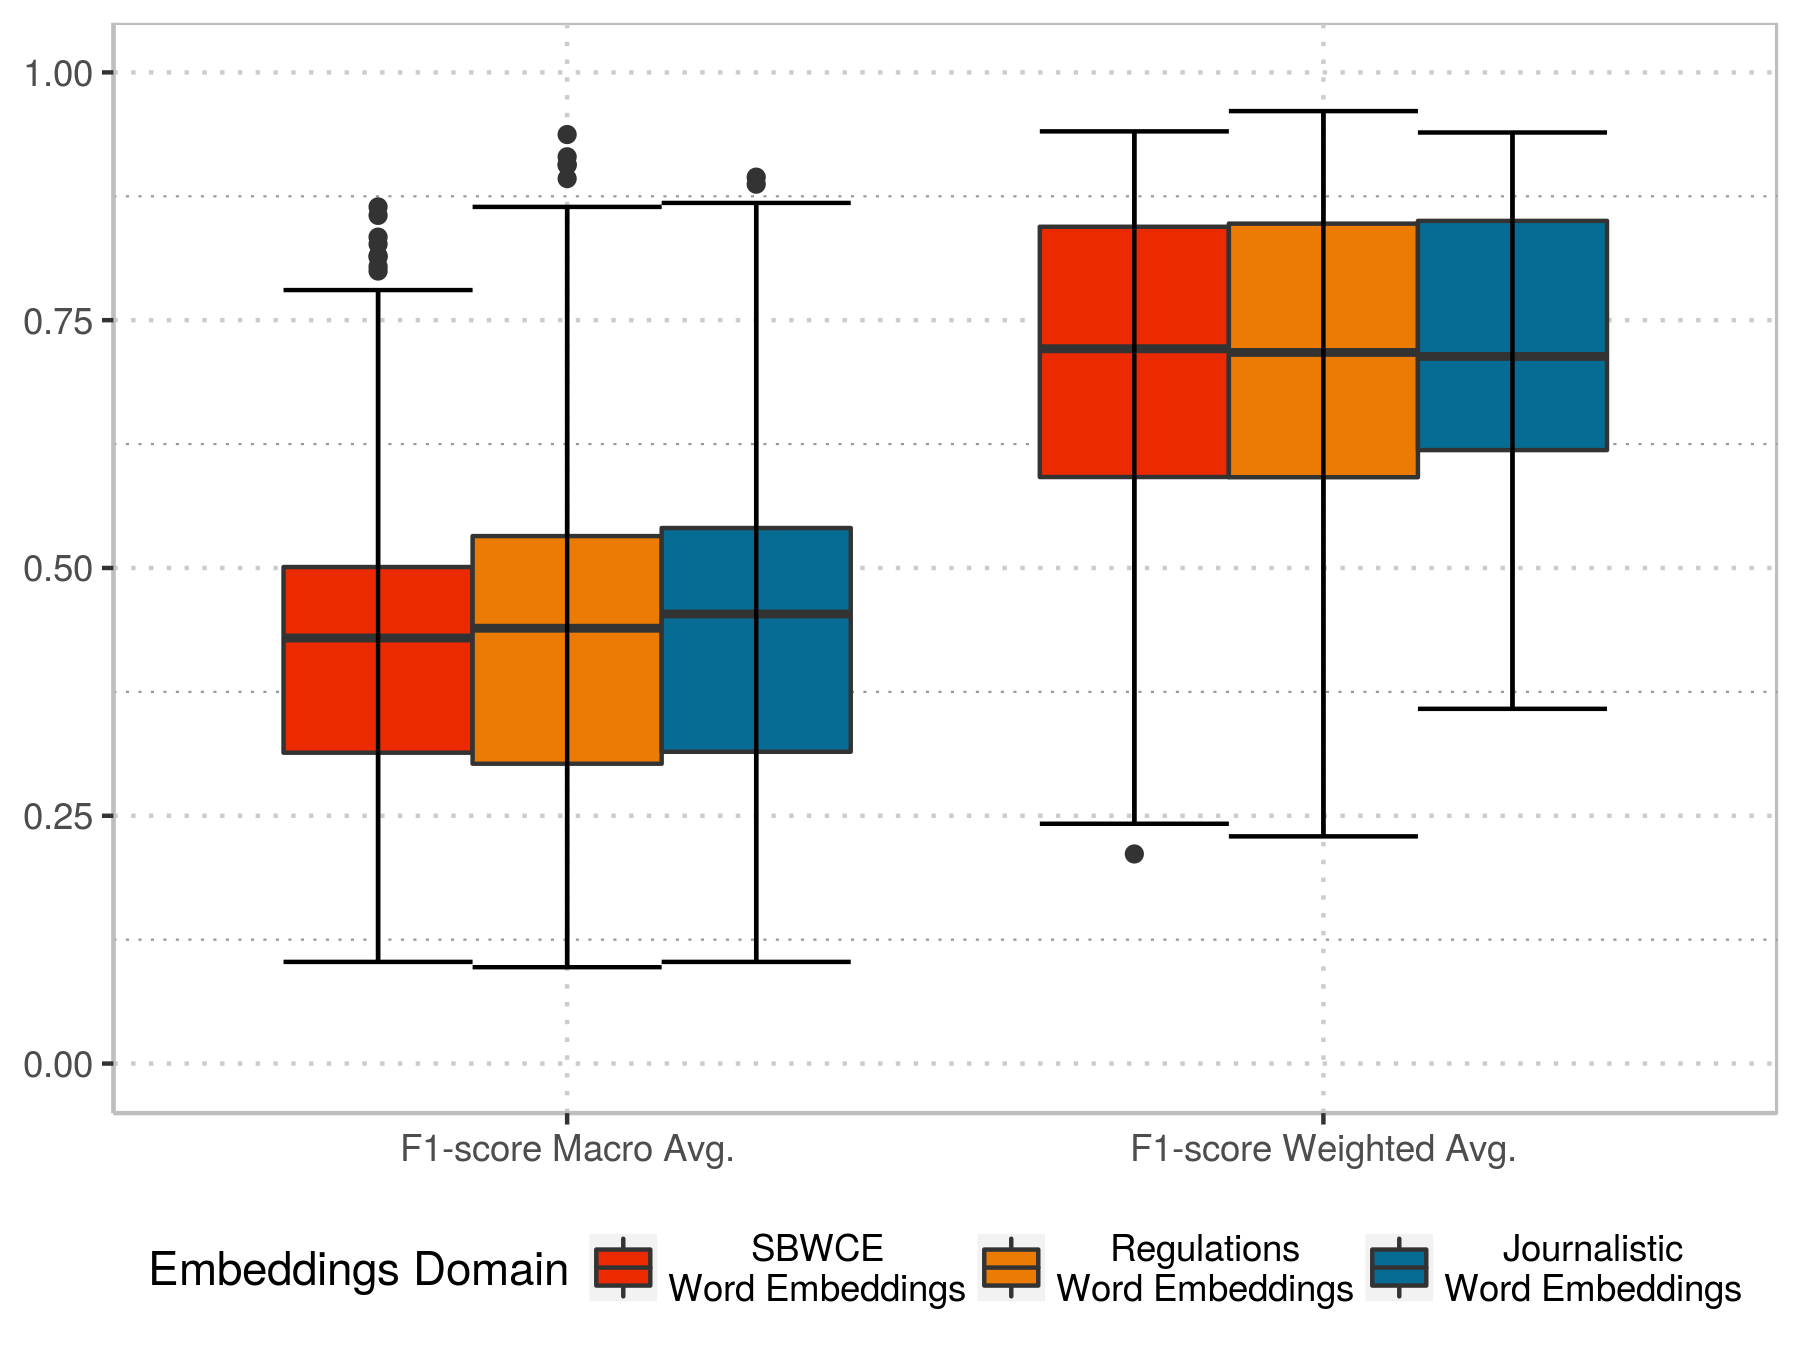
\includegraphics[width=\textwidth]{plots/embeddings/general_vs_out_domain}
  \caption{Performance per lemma on the test corpus for general, specific
  in-domain, and specific out-of-domain embeddings.}
  \label{fig:embeddings:performance_general_out}
\end{figure}

Figure \ref{fig:embeddings:performance_general_out} reports the performance
results on the test corpus for each lemma using these three different domains
to train the word embeddings. The plot is a box and whiskers plot structured in
the following way:

\begin{itemize}
  \item Each group of box-plots shows the different metrics: F1-score macro
    and weighted average.
  \item Each box-plot of a different color shows the performance for
    different training domains of word embeddings: general domain (SBWCE),
    specific domain outside the task (Regulations), and specific domain of the
    task (Journalistic).
  \item The box and whiskers plots represent the distribution of the values of
    the metrics through their quartiles. Each value is the performance for a
    lemma of the corpus. The black thick line in the middle of a box-plot
    represents the median and the whiskers at the end of each box-plot
    represents maximum and minimum value (except for eventual outliers
    represented by black dots outside the box-plot).
\end{itemize}

From the figure, it is noticeable the increase in performance of the median of
the experiments with journalistic, in-domain word embeddings with the F1-score
macro average. Besides the better median, the maximum values are also higher
for in-domain embeddings than for general domain embeddings. In the case of
the F1-score weighted average there is less error  for in-domain embeddings
than for general or out-of-domain embeddings, and the difference for the median
in favor of the general corpus is marginal. Recall that the macro average is
good to measure the performance for the minority classes. Since it is clearly
better for the journalistic in-domain word embeddings, it shows that in-domain
specific word embeddings model less frequent senses better. 

On the other hand it is not clear if the regulations out-of-domain embeddings
affect performance negatively or positively. They show better performance in
some of the better models and worse in some of the worse models, as is
reflected in a wider spread of the whiskers. Thus, I find a clear sign that I
need a close look to each model and see in particular which are the lemmas that
are doing better and which are the ones doing worse. In particular, I need to
look into the outliers. The plot shows that there are 4 (or maybe 5) lemmas
which have better performance with out-of-domain embeddings than with in-domain
embeddings. In any case the journalistic word embeddings are still better in
the general terms for both metrics, because they reduce error.

The reasons behind this results can be many. As a first explanation, the
regulation corpus may not be as dissimilar to the journalistic domain as I
would have expected a priori. A better corpus to test this hypothesis might be
one based in documentation which can be very technical. However, the available
corpus to train such an embedding, at this stage, was not big enough. A line of
future work is to obtain more documentation via web scrapping and train an
embedding from that.

Another possible explanation, which requires the analysis from the point of
view of a linguist expert, is that there are some lemmas (and thus some models)
which show better performance in the particular domain of regulations and thus
this is reflected in the results. This better performance may be due to a
higher frequency in the regulations corpus of words that are relevant to
distinguish senses for that lemma. This line of work will be pursued in future
research.

Finally, the SBWCE has some noise due to the size of the corpus, another line
of future work can be in that area, with embeddings trained from a cleaner
version of the SBWCE.

From these results I have strong evidence to accept the Hypothesis statement,
as the domain from where the word embeddings are trained effectively affects
the final performance of a model.

\subsection{Performance comparison of supervised and semi-supervised
representations}\label{sec:embeddings:results:supvsem}

Hypothesis \ref{hyp:embeddings:2} states that using word embeddings
produces less tendency to overfit over supervised models. Next section reports
the results regarding that hypothesis in order to accept it or reject it.
However, so far I have only compared the results of different word embeddings
for the models.

In this Section, before showing the results of the experiments for Hypothesis
\ref{hyp:embeddings:2}, I want to show how these new models perform in
comparison to the models selected in Chapter \ref{chapter:supervised}. Recall
the final model I want to compare is the multilayer perceptron classifier with
three layers.

Again I follow the steps of Experiment \ref{exp:embeddings:1} that trains a
model with the whole dataset and evaluates such model in a test dataset. For
these results the chosen representations are the hashed hand-crafted features
for the supervised approach and the specific (journalistic) domain word
embeddings for the unsupervised approach.

\begin{figure}[ht]
	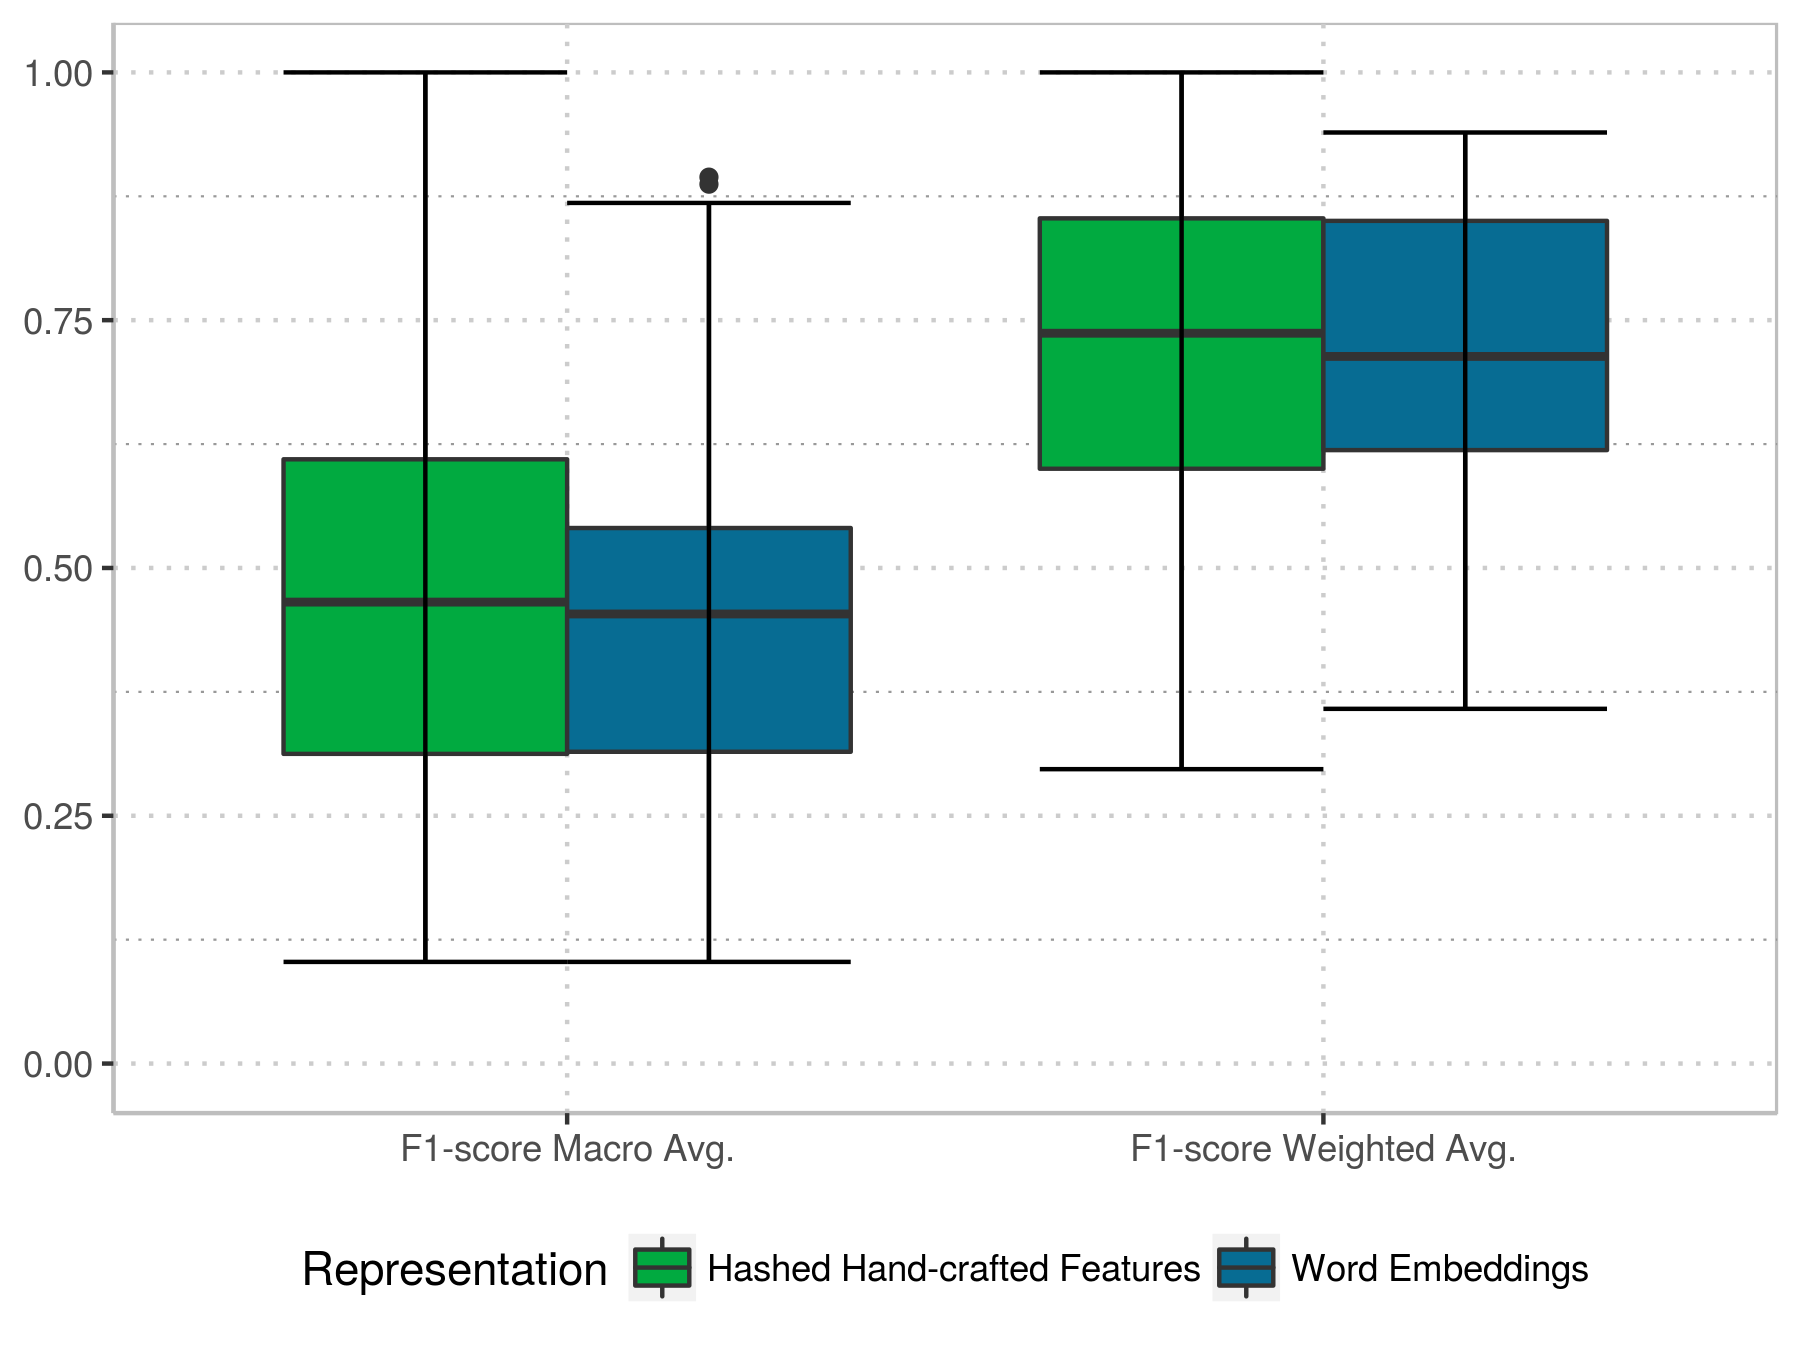
\includegraphics[width=\textwidth]{plots/embeddings/supervised_embeddings}
  \caption{Performance per lemma on the test corpus for hashed hand-crafted
  features and word embeddings of specific domain}
  \label{fig:embeddings:performance_supervised_embeddings}
\end{figure}

Figure \ref{fig:embeddings:performance_supervised_embeddings} reports
the results of Experiment \ref{exp:embeddings:1} and testing it in the held
out test dataset. As in previous Figures, it uses a box and whiskers plot to
display the distribution of the results for each model:

\begin{itemize}
  \item Each group of box-plots shows the different metrics: F1-score macro
    and weighted average.
  \item Each box-plot of a different color shows the performance for different
    representations. For the supervised representation I use the hand-crafted
    hashed features. For the unsupervised representations I use a specific
    domain of the task (Journalistic).
  \item The box and whiskers plots represent the distribution of the values of
    the metrics through their quartiles. The same as explained for Figure
    \ref{fig:embeddings:performance_supervised_embeddings}.
\end{itemize}

In Figure \ref{fig:embeddings:performance_supervised_embeddings} it can
be seen a clear advantage of hashed hand-crafted features over word embeddings.
F1-score macro average performs specially better, indicating that those senses
with low occurrence count are better represented. 

Word embeddings serve as a way of smoothing features by reducing the
dimensionality to a lower, more general representation. Besides, the
representation from which the embeddings are obtained takes into account less
features than hand-crafted features. Indeed, hand-crafted features encode
syntactic and PoS information, while to obtain word embeddings only word
co-occurrences are used.

Taking this into account, it can be interpreted that hand-crafted features
represent the domain better than the semi-supervised model. This may be due to
the fact that the features are taken from the supervised data itself, unlike
the journalistic word embeddings, which are taken from a corpus that shares
domain with the supervised data. Supervised features have a better performance
because they can fit more closely to the data, and that is the reason why
supervised features are less able to generalize a model, specially a domain
driven model, into data from more general domain. In the next section I will
explore the tendency of these models to overfit or generalize.

The adequacy of these two kinds of models to adapt to an out-of-domain corpus
will be displayed in the following Chapter. There we will see that word
embeddings are able to perform well on a self-learning approach on a big
corpus. In contrast, hand-crafted features fail to generalize and their
performance quickly degrades across iterations.

\subsection{Hypothesis \ref{hyp:embeddings:2}}\label{sec:embeddings:hyp:2}

The results of the previous section showed that supervised features perform
better than unsupervised features for the \vsd~task. The results of the
experiments for Hypothesis \ref{hyp:embeddings:2} give a hint on what is
happening underneath these results.

These results are taken from Experiment \ref{exp:embeddings:2}, and report the
learning curve of a model as the number of examples increases. It shows the
mean and error due to variance of both the training and test sets on each
iteration. The comparison is done using a supervised representation via hashed
hand-crafted features and an unsupervised representation via word embeddings,
in this case the specific domain word embeddings.

\begin{figure}[ht]
	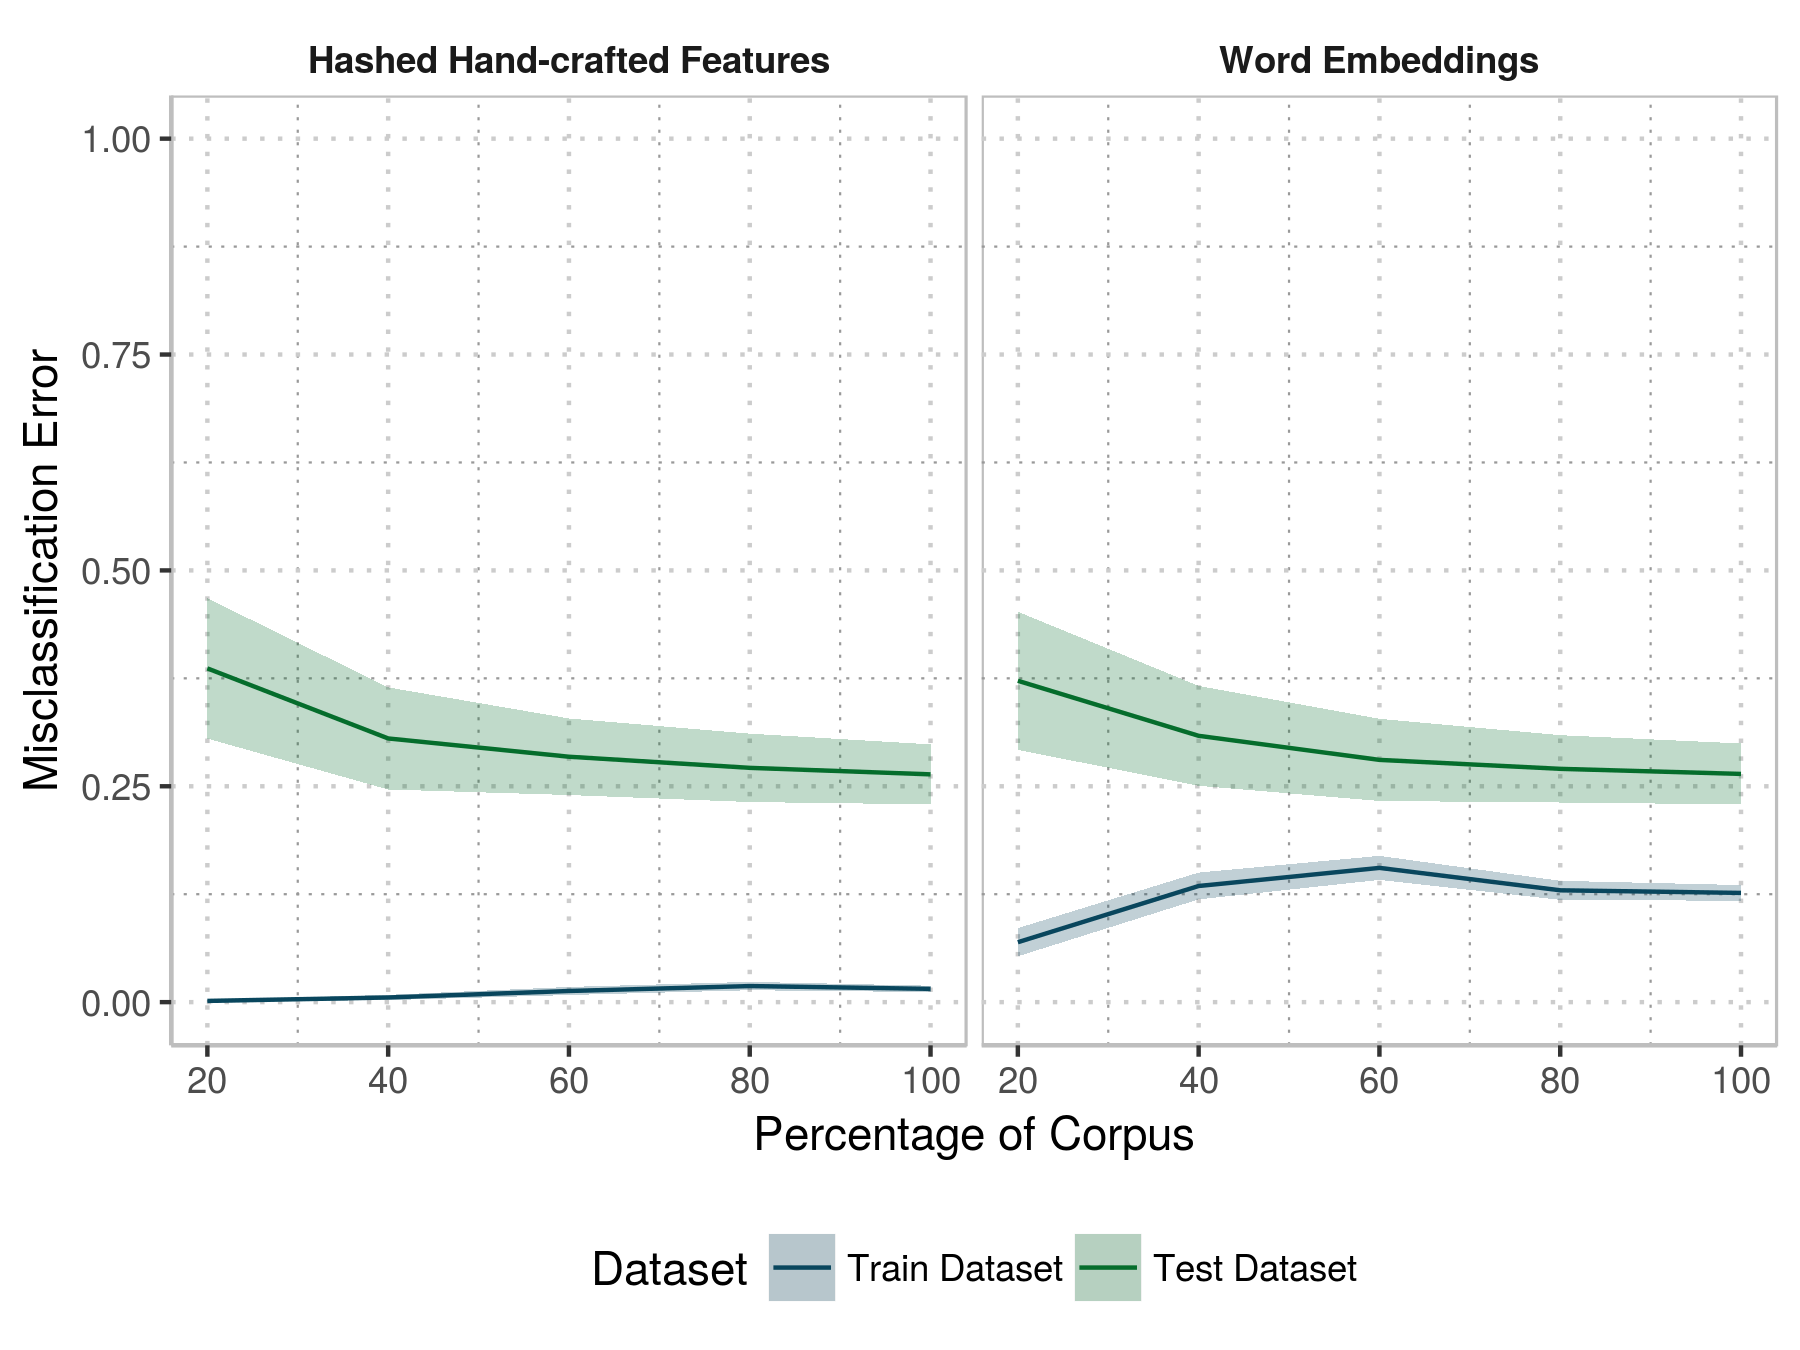
\includegraphics[width=\textwidth]{plots/embeddings/learning_curve_scores}
  \caption{Learning curve for different sizes of training corpus for supervised
  and unsupervised representations}
  \label{fig:embeddings:learning_curve}
\end{figure}

Figure \ref{fig:embeddings:learning_curve} shows the learning curve for
different sizes of the training data over two different representations for the
input features: supervised hand-crafted features and unsupervised word
embeddings. The structure of the learning curve plot is as follows:

\begin{itemize}
  \item The plot is divided in two columns, each represents an input to the
    model: supervised hand-crafted features and unsupervised word embeddings of
    the specific domain (journalistic).
  \item The x-coordinate shows the size of the training data, as a percentage
    of the total training data available, starting from 20\% of the corpus (the
    corpus was split in 5 parts according to Experiment
    \ref{exp:embeddings:2}).
  \item The y-coordinate shows the misclassification error of a model.
  \item There are two colors representing the datasets: train and test.
  \item The solid darker lines represent the mean of misclassification error
    trough the different splits of the datasets over all the models.
  \item The shadowed area, which has a lighter color, represent the standard
    error of the mean of the misclassification error.
\end{itemize}

It is possible to see in the Figure the difference between representations when
the tendency to overfit is measured. Word embeddings show less difference
between the training data and the test data regarding misclassification. This
could also be seen in Section \ref{sec:supervised:hyp:4}, where SVM and Naive
Bayes showed less tendency to overfit the model.

In this case the classifier is a non linear classifier with a strong tendency
to overfit, and the word embeddings are helping it to not overfit as much as
the supervised representation does. Still, it is important to note that the
misclassification error in test data is still roughly the same for one
representation or the other, thus the model is not sacrificing training
performance in order to gain test performance. What the model is actually
sacrificing is anecdotal, non-generalizing information. These results support
evidence to accept Hypothesis \ref{hyp:embeddings:2}. 

It is important to recall that the models are small and neural networks models
work better the more information they have. In order to gather more
information, more examples are needed. However, manual annotation of examples
is expensive and beyond my possibilities. Thus I pursue increasing the number
of examples available to the model via incorporating examples from unsupervised
corpora. And to do so we need models which generalize better to out-of-domain
corpora, as is the case of models with word embeddings. 

\section{Conclusions}\label{sec:embeddings:conclusions}

This chapter introduced a disjoint semi-supervised technique for Spanish \vsd.
From the challenges stated in Chapter \ref{chapter:supervised} I wanted to
overcome the shortcoming of having a model with a high tendency to overfit the
data. I stated a main hypothesis I want to test, which is that unsupervised
representations help improve upon purely supervised models by reducing the
tendency to overfit given by features taken from the same data where the model
is trained. The reason to state this hypothesis is that unsupervised
representations give a smoothed version as input to a classifier and thus this
helps the classifier in having a more generalized version of the data it is
learning from. I subdivided the hypothesis in smaller, more focused
subhypotheses.

Hypothesis \ref{hyp:embeddings:1} states that the performance of an
unsupervised representation, in this case a word embedding, depends on the
domain from where the unlabeled data to train the embeddings is taken. The
results to accept this hypothesis are in Section
\ref{sec:embeddings:hyp:1}. It was shown that a more specific domain gives
better results for the same task. Still some of the results regarding the use
of a domain outside the domain of the supervised need a more thorough analysis
left for future work.

Before analyzing the results of the experiments to test Hypothesis
\ref{hyp:embeddings:2} I needed a comparison between supervised and
unsupervised representations. This is reported in Section
\ref{sec:embeddings:results:supvsem}. In this experiment I train two
different models using the neural network classifier with three layers
described in Section \ref{sec:embeddings:classifiers}, and changing the
input representation for the classifier. From this comparison, hand-crafted
features show better performance than the unsupervised features. However the
reason behind this is that hand-crafted features obtain a more fitted
representation  of the supervised dataset as the features come directly from
there. The results of the experiments to test Hypothesis
\ref{hyp:embeddings:2} show that hand-crafted features are strongly
dependent on the dataset, and that the resulting representation is highly
fitted to the training examples.

Section \ref{sec:embeddings:hyp:2} shows the results of Experiment
\ref{exp:embeddings:2}, which measures the tendency to overfit of a
classifier. The experiment is done to test Hypothesis
\ref{hyp:embeddings:2}, which states that unsupervised representations
(e.g. word embeddings) produce less overfitting over the supervised models than
supervised representations (e.g. hand-crafted features). The experiment
compared hashed hand-crafted features and specific domain word embeddings. As
the hypothesis states, the model trained with word embeddings showed a closer
learning curve between training and test data. This gives enough evidence to
support the acceptance of Hypothesis \ref{hyp:embeddings:2}.

Unsupervised feature representations, particularly those trained from the same
domain as the supervised dataset, show promising results. However, the
performance is still under what I can achieve using purely supervised
representations. And although there can be many reasons to explain this result,
according to what I see, most likely it has to do with the (over)fitting of the
supervised features to the supervised data, in contrast to the more smooth
representation of word embeddings.

Recall from the previous Chapter I found two main challenges. The first
challenge was that models trained with little data tend to overfit. Using
non-linear classifiers such as neural networks could have a great impact in
minimizing the error and even maximizing the performance of the test data. But
the cost is the generalization of such models. Unsupervised features help in
that respect by giving a smoother representation helping the neural network to
avoid the tendency to overfit.

The other challenge was the coverage of the model. Coverage can be understood
as the ability to predict over unseen examples that belong to one of the target
classes and the model should be able to label. These examples could eventually
be incorporated to the training corpus and thus add information to the model.
But since they are not annotated, the model does not have such information yet.
Given our limitations to annotate examples manually, new examples are gathered
from unlabeled data and classified with the model. If the model is only driven
by the information it already has (i.e. the features extracted from the
supervised data), then is difficult to add the information from unseen data and
expand the coverage. Word embeddings hold information about the supervised
data, used for the model to classify it, and about unsupervised data not
present in the model yet. Thus, this information helps a model trained from
unsupervised features generalize better and be able to gather information from
new examples expanding its coverage.

Following these reasons, word embeddings seem specially adequate to apply an
approach to obtain new examples from previously unseen corpus.

In the next chapter I will focus on a first approach to a semi-supervised
method which adds data from unlabeled sources and use that to expand the model.
Such method is self-learning, a basic approach to semi-supervised learning.

Future work of this chapter includes using other unsupervised representations,
like the ones listed by Turian et al. \cite{Turian:2010:WRS:1858681.1858721}:
Collobert and Weston \cite{Collobert:2008:UAN:1390156.1390177} and Brown
clusters \cite{Brown:1992:CNG:176313.176316}. Another line of work would be
doing a more thorough error analysis on the the different word embeddings
domain, seeing if a better preprocessing of the data can provide better
results. 


\part{Joint Semi-Supervised Methods}

\chapter{Self-Learning}\label{chapter:self-learning}
\section{Overview}

With a task like Spanish \vsd, where the annotated data is small, a purely
supervised approach has to overcome two challenges: the model overfits the
data, and the model's coverage is small. These were the findings of Chapter
\ref{chapter:supervised}. Chapter \ref{chapter:embeddings} explored a
semi-supervised approach by providing word embeddings as input to a supervised
classifier.

The results of the previous chapter gave evidence in favor of Hypothesis
\label{hyp:embeddings:3}. Recall the hypothesis states that word embeddings had
less tendency to overfit than supervised features. The results served to accept
this hypothesis. However, this improvement in overfitting came with a decrease
in performance: supervised features adapted better to the problem, word
embeddings performed worse. Still the results of word embeddings were
promising, because having less overfitting implies a better performance in
general domain corpora.

The other challenge for this task was coverage. Coverage can be thought of as
the unseen examples, part of a class, that the model can reach (i.e. classify
to the correct class). Examples not in training could add information to the
model that is not integrated in the model yet. One way to add such information
is by adding previously unseen examples to the model. Word embeddings help in
this direction, not by adding new examples to the model, but by adding
information from unlabeled data. With this additional information, the model is
able to cover a wider range of examples.

To increment the model coverage with new examples I explore {\em
self-learning}. This is a semi-supervised technique that expands labeled data
by using the certainty of the model over unlabeled data. It adds new examples
automatically, using a supervised model to label unlabeled examples.  This is a
{\em joint semi-supervised learning} algorithm. This means that labeled and
unlabeled data are used jointly in the process of learning. In contrast, the
approach with word embeddings is {\em disjoint} because embeddings are obtained
independently from the model for \vsd.

The self-learning algorithm works basically as follows. A supervised algorithm
is trained on a seed labeled dataset. Then the obtained model is used to
classify unlabeled examples obtained from a big unlabeled corpus. The certainty
of the algorithm in classification is used to add automatically labeled
examples to the labeled dataset. The algorithm uses this bigger dataset (coming
from both supervised and unsupervised data) to train a new model. This process
is iterated until a stopping criterion is met.

In general terms, self-learning is a simple algorithm that applies a {\em
bootstrap technique} to improve on a supervised model that improves with
unlabeled data. The objective of exploring this technique relies on
incrementing the model coverage as I said before. The underlying assumption is
that the new examples will help the model integrate the information that is
latent on those examples.

However there is a challenge I need to face when coming to train a model using
a self-learning approach. This challenge resides in the imbalance of the
classes in the corpus. If the initial model is biased to classify the instances
as part of the most common class, this error will be dragged by the
self-learning model and will automatically annotate new examples as the most
frequent class just because the original model does so. 

Moreover, in this particular case there is another problem, and that is the
specific domain of the corpus on which the initial model is trained. Recall
that SenSem, the resource I am basing the experiments on, comes from a specific
domain: journalistic. Having a biased domain also affects which classes appear
the most. Thus some classes are the most common in a general domain but this is
not the case for the specific domain as the next examples illustrates:

\begin{example}
  The verb ``llegar'' has 8 different senses in SenSem. Of them, one is ``to
  reach certain height or point''. This sense is not the most common one
  available in the SenSem corpus as it has a few labeled examples in the
  corpus. However in a more broad domain it can be used with a higher
  prevalence than in this domain.
\end{example}

These are the reasons behind studying different techniques in the previous
chapters to avoid overfitting and bias to the most frequent class in the
supervised algorithm. This is important for the self-learning algorithm to
avoid diverging to the most frequent class too quickly and thus not adding
enough useful, diverse information to the model.

This chapter will test the following hypothesis:

\begin{hypothesis}\label{hyp:self-learning}
  The target classes of a model trained on labeled data can be better
  represented by integrating more examples, even if they are automatically
  labeled (and thus contain error and bias). Increasing the number of examples
  to train a model helps to avoid overfitting of the model and improves
  coverage.
\end{hypothesis}

In order to accept or reject such Hypothesis, I divide it in more specific
ones. 

First I make two hypotheses about the general goodness of this approach to
improve upon a mostly supervised approach:

\begin{subhypothesis}\label{hyp:self-learning:1}
  The performance of the model over the held-out test data improves after the
  self-learning algorithm adds new automatically annotated examples.
\end{subhypothesis}

\begin{subhypothesis}\label{hyp:self-learning:2}
  The model obtained in each iteration shows an increase in the average
  certainty to predict the class of unseen examples. 
\end{subhypothesis}

Concerning overfitting, I make the following hypothesis:

\begin{subhypothesis}\label{hyp:self-learning:3}
  Increasing the number of examples helps reducing overfitting.
\end{subhypothesis}

Concerning coverage, I make the following hypothesis: 

\begin{subhypothesis}\label{hyp:self-learning:4}
  The self-learning algorithm increases the number of features associated to
  the model, which is an indicator of an increment in the coverage of the
  model.
\end{subhypothesis} 

Given the initial bias in the distribution of classes and the bias of the
self-learning algorithm to amplify this initial bias and overpopulate a
majority class, the following hypotheses are expected to be rejected:

\begin{subhypothesis}\label{hyp:self-learning:5}
  Self-learning helps improving the performance of the model on each of the
  classes uniformly.
\end{subhypothesis}

\begin{subhypothesis}\label{hyp:self-learning:6}
  The representativity of each class in the dataset is kept through all
  iterations of the algorithm.
\end{subhypothesis}

\begin{subhypothesis}\label{hyp:self-learning:7}
  The coverage of the features is uniformly distributed across classes.
\end{subhypothesis}

These hypotheses will be accepted or rejected using the following layout:

\begin{itemize}
  \item Experiment \ref{exp:self-learning:1} reports the performance of a model
    before and after running the self-learning algorithm. The performance is
    measured by the macro and weighted average F1-score (Metric \ref{met:1}).
    Results shown in Section \ref{sec:self-learning:hyp:1} serve to test and
    mildly reject Hypothesis \ref{hyp:self-learning:1}, that the performance
    over a model on held-out test data improves after the self-learning
    iterations.
  \item Experiment \ref{exp:self-learning:2} shows the certainty the model over
    predicted classes for each iteration of the algorithm. The average of this
    value is what I need to test Hypothesis \ref{hyp:self-learning:2} which
    states that the model has an increase in the average certainty along
    self-learning iterations (Metric \ref{met:5}). The results of this
    experimentation are shown on Section \ref{sec:self-learning:hyp:2} and show
    that certainty is not increased, thus this Hypothesis is rejected.
  \item Experiment \ref{exp:self-learning:3} assesses overfitting by measuring
    the error due to variance of a model trained on one dataset over other
    datasets. To measure this I use the learning curve (Metric \ref{met:3}) I
    already explained in previous chapters. The results of the experiments
    shown in Section \ref{sec:self-learning:hyp:3} serve to mildly reject
    Hypothesis \ref{hyp:self-learning:3} which states that adding new examples
    to the dataset helps to decrease the model tendency to overfit. 
  \item Experiment \ref{exp:self-learning:4} records the number of features a
    model has. This number of features is measured by raw count. Results shown
    in Section \ref{sec:self-learning:hyp:4} serve to accept Hypothesis
    \ref{hyp:self-learning:4} that the self-learning algorithm increases the
    number of features associated to the model.
  \item Experiment \ref{exp:self-learning:1} also serves as the base to test
    Hypothesis \ref{hyp:self-learning:5}, that the self-learning algorithm
    improves the performance of each class uniformly. To test this hypothesis I
    look at the results from a different perspective. Section
    \ref{sec:self-learning:hyp:5} discusses the results regarding this
    hypothesis. This time however I do not use the average of F1-score (Metric
    \ref{met:1}), but rather the F1-score of each class before and after the
    self-learning iteration. Results show that, as expected, the hypothesis is
    rejected.
  \item Experiment \ref{exp:self-learning:5} records the distribution of the
    classes in the training dataset for each of the iterations in the
    self-learning algorithm. This distribution is measured by the proportional
    count of such classes. The results of this experiment measured with the
    metric are displayed in Section \ref{sec:self-learning:hyp:6} and serve to
    reject Hypothesis \ref{hyp:self-learning:6} of the classes being uniformly
    distributed across self-learning iterations.
  \item Experiment \ref{exp:self-learning:4} is also used, measured differently
    this time, to test Hypothesis \ref{hyp:self-learning:7}. The experiment
    collects the number of times a feature and a class co-occur in the training
    dataset. These results are measured by two different metrics. First the raw
    count of features per class. On the other hand I also look into the
    association each class has to each feature. To do this I use the pointwise
    mutual information defined in Metric \ref{met:4}. The results that serve to
    reject the Hypothesis are shown on Section \ref{sec:self-learning:hyp:7}.
\end{itemize}

In Section \ref{sec:self-learning:previous} I revise some previous work done in
self-learning in general and also specifically applied to \vsd. Also I mention
some other semi-supervised methods based on bootstrap techniques.

In Section \ref{sec:self-learning:methodology} I go through the relevant items
that concern to the experimentation done in the chapter. Section
\ref{sec:self-learning:resources} reintroduces the resources I work with in the
experimentation. Most of them were already introduced and I only do a quick
summary with references to the section where the resource is better explained.
Next in Section \ref{sec:self-learning:features} I explain the features and
representations I work with in this chapter, and particularly give some hints
on how to deal with the add of new examples by the model and how this affects
the representation by adding new features as well. Section
\ref{sec:self-learning:algorithm} explains the fine detail of the self-learning
algorithm, including certainty threshold and stopping criterion the algorithm
uses. Finally Sections \ref{sec:self-learning:experiments} and
\ref{sec:self-learning:metrics}, as in previous chapters, lists the experiments
and metrics I use to measure the results respectively.

Section \ref{sec:self-learning:results} reports the results of the experiments
and analyzes them in order to accept or reject the stated hypotheses of the
chapter.

Finally Section \ref{sec:self-learning:conclusions} draws the conclusions of
this chapter, recapitulating the Hypotheses and the implications of accepting
or rejecting them according to the evidence gathered in the results. It states
the shortcomings of the methods explored in this chapter and what I want to
accomplish on the next. It ends by outlining future work.

\section{Relevant Work}\label{sec:self-learning:previous}

As explained in Section \ref{sec:general_background:self-learning}, of Chapter
\ref{chapter:general_background}, self-learning is one of the first approaches
in using a semi-supervised learning technique with quite some time in the
literature \cite{Scudder:2006:PEA:2263254.2267291}. The idea has been applied
in many natural language tasks besides \wsd: subjectiveness in nouns
\cite{Riloff:2003:LSN:1119176.1119180}, dialogue classification
\cite{Maeireizo:2004:CPE:1219044.1219072}.

For self-learning applied to \wsd, the work of Yarowsky \cite{yarowsky-95} to
build a disambiguation model based on the words co-occurring with manually
labeled examples is fundamental in the area. The exploration done in this
chapter takes most of its ideas from this work. Another work is the one by
Mihalcea \cite{mihalcea:2004:CONLL}, on which she explores the different
settings of hyperparameters one can have in the algorithm to improve the
performance of the supervised task.

\section{Methodology}\label{sec:self-learning:methodology}

This chapter explores the self-learning algorithm to expand a supervised model
with unlabeled data annotated automatically based on certainty. The
self-learning algorithm is a {\em wrapper}. This means the self-learning
algorithm does not classify data by itself. It does it by wrapping a supervised
classifier. Then it uses the information the supervised classifier gets from
the data to augment the model.

Recall that independent classifiers are learnt for each lemma. I describe the
methodology in general terms, but I still run one self-learning algorithm model
per each lemma. It is important to keep in mind that evaluation metrics may
obscure differences in performance across lemmas.

\subsection{Resources}\label{sec:self-learning:resources}

Self-learning requires two main resources: a labeled and an unlabeled dataset.
The labeled dataset is the seed of the initial model. From this data the
algorithm bootstraps the iterations. The unlabeled dataset is the source of new
examples to annotate automatically. The experimentation for this chapter is
done only on the Spanish corpora.

Initially I wanted to do a general analysis of the results of \vsd~for all the
available lemmas. However, while working on the analysis, giving a much closer
look to the data, it was concluded the best method was to take some token
lemmas and analyze them with a much closer look to see how the algorithm works
on each of those cases. Besides this, the other reason to do so was to have
some point of comparison when doing active learning in the following chapter as
the availability to manually labeled data was limited.

As token lemmas, I selected a communication verb, originally ``hablar'' was
intended, but there were annotated examples of only one sense, thus
``explicar'' was chosen instead. I also selected ``pensar'', another verb of
the communication class, to observe similarities and differences. Two verbs of
movement were next: ``acceder'' and ``llegar''. Finally two transitive verbs
were selected: ``buscar'' and ``facilitar''.

\subsubsection{SenSem}

The SenSem corpus is used as the annotated seed on which the self-learning
algorithm starts. For more information on this resource please refer to Section
\ref{sec:supervised:sensem}.

The main problem with using SenSem as it is in self-learning is how it is
affected by the algorithm's tendency to diverge to the most frequent class. As
I will show in the results further in this chapter, this is a big problem
regarding self-learning. A first approach I had to follow in order to deal with
this problem was oversampling.

I randomly oversampled the examples of the less frequent classes in order for
the initial (seed) dataset had an equivalent number of examples for each class.
This did not completely fixed the algorithm's tendency to classify everything
as part of the most frequent class, but it did help in smoothing this. If I
used in the experiments the original dataset without oversampling then the
algorithm's drifting was much more quicker. This oversampling had no impact on
the performance of the supervised algorithm (i.e. the classifier trained only
on labeled data) over the test corpus, but did help in the case of the
self-learning iterations to delay the drifting to the most frequent class.

\subsubsection{SBWCE}\label{sec:self-learning:sbwce}.

The unlabeled data source of new instances for the algorithm is the SBWCE.
This resource was already described in Chapter \ref{chapter:embeddings},
Section \ref{sec:embeddings:sbwce}.

Due to time and resources constrains I was not able to use the full resource.
The algorithm takes and classifies the unlabeled data to select the instances.
Then with the full SBWCE dataset each iteration would take a large amount of
time to complete. The solution was to randomly sample a fixed number of
unlabeled sentences for each lemma. For each lemma I chose 1000 unlabeled
sentences and used them as unlabeled data for self-learning.

Once the sentences were selected the corpus is preprocessed to add PoS and
dependency annotations. The preprocessing step is done with Freeling. The key
idea is to have in the unlabeled dataset the same type of information as the
supervised dataset, as described in~\ref{sec:supervised:sensem}. This
information is used to build the hand-crafted features.

\subsection{Features}\label{sec:self-learning:features}

The previous chapter showed that word embeddings are promising but supervised
features still have the best performance. I decided to keep both kinds of
features and compare how each performs on jointly semi-supervised learning
tasks. Parameters for both kinds of representations are the ones with the best
performance in previous chapters.

\subsubsection{Hand-crafted features}\label{sec:self-learning:handcrafted}

For hand-crafted features I use the features described in Chapter
\ref{chapter:supervised}, Section \ref{sec:supervised:features}. 

Recall the whole set of hand-crafted features for the supervised data was
already large even though the labeled dataset was small. When this is done for
unlabeled datasets the amount of features are most likely too big to fit in
memory.

Moreover, the original supervised model of the self-learning algorithm is
trained only on the supervised data. Then it only has the features the
supervised corpus has. These features are not likely to be the only ones
available in the unlabeled dataset.

As most of the classifiers take a fixed size input, having new features from
unlabeled data gives two options: ignore the features or generate a
representation with the features of the whole dataset (i.e. labeled and
unlabeled).

Feature hashing, described in detail in Section \ref{sec:supervised:hashing},
gives a very efficient solution to this problem. It was developed with online
learning in consideration where the labeled data is ongoing.

\subsubsection{Word embeddings}

In Chapter \ref{chapter:embeddings} I conclude from the experimentation that
the domain of the word embeddings affected the performance of the model. For
these experiments I selected the word embeddings that showed the best results
in the previous chapter. This are the ones obtained from the journalistic
corpus described in Section \ref{sec:embeddings:resources}. The embeddings
were trained using word2vec and the instances are constructed by concatenation
of the embeddings, the process is described in Section
\ref{sec:embeddings:embeddings}.

\subsection{Classifiers}

In the next Section I describe the details of the self-learning algorithm.
However recall this is a wrapper method. Then I still need a supervised
classifier to use as parameter of the self-learning model. The classifier is an
hyperparameter of the self-learning algorithm.

Based on the results of Chapter \ref{chapter:supervised} I selected the
multilayer perceptron with three layers of size 500, 250 and 100. For the
chapter all the experiments have this classifier fixed.

\subsection{Self-learning algorithm}\label{sec:self-learning:algorithm}

As I explained before, the self-learning algorithm is a wrapper algorithm over
a classifier. The algorithm takes the following initial parameters:

\begin{itemize}
  \item A labeled training dataset to train the initial supervised model.
  \item A labeled test dataset to report the model performance before and after
    finishing all the iterations of the self-learning algorithm.
  \item A labeled validation dataset to keep track of the self-learning
    algorithm automatically added instances and avoid divergence of the
    original model.
  \item An unlabeled dataset to get the new data to annotate automatically.
  \item A probabilistic classification algorithm, to use in the process of
    automatic annotation.
  \item A tolerance error for the stopping criterion.
\end{itemize}

The labeled test dataset is the same one used in the experiments of previous
chapters. The validation dataset is taken from the training dataset following
the same structure as described in Section \ref{sec:supervised:sensem}. The
SenSem corpus was split with 80\% for training and 20\% for test, but keeping
at least one instance for each class (sense) in test dataset and two instances
in the training dataset. The validation dataset was taken from the training
dataset by splitting it again into 80\%-20\%. This split was also ensuring
there was at least one example for training and one example for validation for
each class in the dataset. 

As with the training/test splits, the training/validation splits also preserve
the distribution of classes observed in the whole dataset. This implies that in
each split you cannot find more examples of a class than you could find in a
stratified sample of the dataset, that is, a sample that preserves the
distribution of the whole dataset. However, this does not necessarily hold for
minority classes, because at least one example must be found in each split,
even if that implies over-representing the class.

The algorithm starts by training an initial model from the labeled training
data. From that model I get the initial performance of the classifier over the
test and the misclassification error of the validation data. The former are
used to compare the model before and after the self-learning iterations. The
latter is used as a stopping criterion for the algorithm.

The self-learning algorithm consists of a loop which uses the trained model to
gather new data from the unlabeled dataset. In the first iteration the model is
the initial one trained with the labeled training data.

On each iteration of the loop the model classifies the whole unlabeled dataset.
From this classification, the algorithm selects the instances to automatically
annotate. These instances are selected based on the certainty (probability) the
classifier has that the instances are part of the class they were classified. 

The certainty of the model over the instances needs to be over a threshold to
be annotated automatically. This threshold is another hyperparameter of the
self-learning algorithm. How I select this threshold is further explained in
the next section.

With the instances and its corresponding labels (given by the classifier),
plus the labeled data collected so far (consisting of the original training
dataset and the new data added after each iteration) the algorithm trains a new
model. The model is tested on the validation dataset to get the
misclassification error. The error can not be larger than the lowest validation
error so far plus the error's tolerance hyperparameter, otherwise the algorithm
stops and the final model is the last model obtained so far. In case the error
is lower than the tolerance, the model is updated for the next iteration. The
selected instances are added as part of the new training set for the next
iteration and removed from the unlabeled dataset.
 
The algorithm continues the loop until the stopping criterion is met or there's
no more data to add. This may happen in two occasions: all the unlabeled data
is already part of the model or the classifier does not have enough certainty
over any of the possible instance to add them to the new model. Once the
algorithm's loop finishes for any reason the last model is used to measure the
performance over the test dataset.

The algorithm has two important parameters: the certainty threshold to add new
examples, and the error tolerance to stop the algorithm before all data is
consumed. There are many ways to set those. In the next two sections I will
further explain my decisions over these two parameters.

\subsubsection{Certainty threshold}

In each iteration of the algorithm after training a new model (i.e. using the
initial training data plus the instances added from previous iterations) the
model is used to gather new training examples from the unlabeled dataset pool.
The classifier is probabilistic, thus it naturally has a certainty over the
data it classifies. This certainty is the probability given to an instance by
the classifier to belong to a certain class. The certainty threshold is the
minimum probability the classifier needs over an instance for the self-learning
algorithm to integrate it as a new training example: any example on which the
classifier has a certainty larger than the threshold are annotated
automatically and added to train a new model. 

On initial experiments the threshold was fixed at the beginning of the
algorithm. The same initial value was used for all the iterations. This value
was the same for all the lemmas. Recall that I have one classifier per lemma to
disambiguate. In this case, I run one set of the algorithm's iterations per
lemma as explained before. Having a fixed threshold for the different lemmas
may not be adequate, as each lemma has its own properties which make it
different from the rest.

Looking for a more adequate solution, the first thing to explore is to define
an initial threshold for the first iteration and adapt it after each step until
a good value is found. However, there are two problems with this approach: how
to set the initial threshold value and how to define a ``good value''
automatically.

Another option is discussed by Mihalcea \cite{mihalcea:2004:CONLL}. She
presents a self-training algorithm which selects the top N instances according
to the certainty of the classifier on them and integrates them as new training
examples. Nevertheless, the only way to choose that number N for this case is
empirically. Thus, we still suffer the same problem as with the threshold, the
way to estimate the parameter.

One way or another, I have the same challenge: not being able to define with
enough confidence which values to set for the hyperparameters. Plus, there are
no rules of thumb to do so either. Thus I decided to go with a threshold of
certainty so the algorithm is not limited to add only a fixed number of
elements. Using a threshold, the self-learning algorithm can add all the
elements with high certainty.

To avoid selecting the threshold manually, I decided for the threshold to be
100\% of certainty in each iteration. If there are no instances at this level
of certainty the threshold is lowered by an alpha hyperparameter, in this case
5\%. With the new threshold the algorithm looks for instances. The threshold is
lowered until at least one instance above the threshold is found or the
selection of instances becomes random. Random selection is identified whenever
the certainty threshold is equal to the random chance of selecting a class in
the algorithm (i.e. if the dataset has 2 classes, the threshold is near to
50\%, if the dataset has 3 classes, the threshold is near to 33\%, etc.). When
this is the case the algorithm stops and does not select any instances. In the
implementation, I restrict this stopping criterion further by stopping a 10\%
before the figure for random selection for each lemma.

A more adequate stopping criterion would use the distribution of classes
actually observed in the data instead of a uniform distribution. Further work
will explore this variation of the algorithm.

\subsubsection{Stopping criterion from validation dataset}

Once the instances were selected by the classifier (assuming a selection was
made and the algorithm did not stop because it did not add any examples), their
impact in the model is evaluated. This is the purpose of the validation
dataset. The algorithm trains a new model with the instances and the data
accumulated so far, that is, the original supervised data and the automatically
annotated instances added in previous iterations. With the model obtained the
algorithm gets the misclassification error from evaluation the model on the
validation dataset. The error is compared to the minimum misclassification
error obtained so far plus a tolerance. Similarly to the classification
threshold, the error tolerance begins in zero and is incremented gradually up
to a maximum misclassification error that is 10\% less than random chance.

The reason to use a validation dataset for the stopping criterion is avoiding
to overfit the model to the test dataset. The parameters and hyperparameters of
the model are adapted this way to the validation dataset. This is also known as
tuning of the model. Afterwards, when the model is evaluated on the test
corpus, results are actually representative.

An alternative approach to this would be {\em k-fold cross-validation} over the
training dataset in each iteration (i.e. the training set with both the labeled
data and the automatically annotated data). Then, the mean misclassification
error could be used as a stopping criterion. However, the tendency of the
algorithm to include more examples of the most frequent class undermines the
adequacy of this approach. Indeed, the misclassification error may get lower
and lower simply because I am evaluating it in a dataset that has grown
unbalanced. Then, when the classifier predicts new instances as belonging to
the most frequent class, there is a higher probability that they are correctly
classified. In contrast, evaluating in a held out test dataset preserves the
original distribution of classes.

\subsection{Experiments}\label{sec:self-learning:experiments}

Recall all the experiments use an oversampled version of the initial labeled
dataset in order to avoid for the dataset to drift to the most frequent class
immediately.

Experiment \ref{exp:self-learning:1} reports the performance of the model over
the test dataset before and after the self-learning iterations. First the
experiment reports the performance of the model trained only with supervised
data. Afterwards it reports the performance of the model trained with the
original supervised data plus the automatically annotated data added by the
self-learning algorithm. Recall all the experiments are done in a per lemma
basis. 

\begin{experiment}\label{exp:self-learning:1}
  \begin{enumexp}
    \item Train a model with the supervised training dataset.
    \item Evaluate the model over the test dataset.
    \item Run the self-learning algorithm until it stops.
    \item Evaluate the model obtained with the self-learning algorithm over the
      test dataset.
  \end{enumexp}
\end{experiment}

Experiment \ref{exp:self-learning:2} keeps track of the average certainty for
each iteration of the self-learning algorithm. The experiment records the
certainty the algorithm has over the classification of the instances.

\begin{experiment}\label{exp:self-learning:2}
  \begin{enumexp}
    \item Start with the self-learning iterations.
    \item Run the model obtained up to this point into the whole unlabeled
      dataset (part of the self-learning algorithm).
    \item Before selecting the instances record the predicted classes for each
      instance and the probability (certainty) they have for the model.
    \item Continue with the self-learning algorithm.
  \end{enumexp}
\end{experiment}

Experiment \ref{exp:self-learning:3} is done to evaluate the {\em error due to
variance} of the model trained by the self-learning algorithm. The objective of
this experiment is to measure the tendency to overfit of a model as the number
of examples increases with the self-learning algorithm. It is based on the
experiments of previous chapters which report the overfitting as well. It
changes however in one fundamental aspect. The previous chapter had to work
with a limited size corpus and showed the learning curve of the experiment by
splitting the dataset. In this case the dataset adds new examples by the design
of the self-learning algorithm. Thus, I measure how these new examples affect
the learning curve. Remember this is done on a per lemma basis. The structure
of the experiment is as follows:

\begin{experiment}\label{exp:self-learning:3}
  \begin{enumexp}
    \item Take only a portion of the whole unsupervised dataset to use as
      instances.
    \item Shuffle both training and validation datasets and split them randomly
      with stratified sampling.
    \item Start the self-learning algorithm.
    \item In each step, train the classifier with the training data obtained
      before starting the training algorithm plus the automatically annotated
      instances.
    \item Record the predictions over training and validation data.
    \item Repeat the whole procedure {\em n} times with a different portion of
      the unsupervised dataset.
  \end{enumexp}
\end{experiment}

The repetition of the procedure {\em n} times emulates what in the previous
chapters was done using the random splitting of the supervised dataset.
Changing the unsupervised dataset and reshuffling and splitting training and
validation datasets evaluates the classifier on new sets of data and shows how
much it varies over different datasets. This is used to generate an estimator
of the model's tendency to overfit.

Experiment \ref{exp:self-learning:4} reports the features associated to the
model. The experiment records the features for each instance of each class.
This displays the number of features the whole model is covering as well as the
number of features for each class.

\begin{experiment}\label{exp:self-learning:4}
  \begin{enumexp}
    \item Record the number of times a tuple $(class, feature)$ occurs for each
      class and each feature of the supervised training dataset.
    \item Run an iteration of the self-learning algorithm.
    \item Record the number of times a tuple $(class, feature)$ occurs for each
      class and each features of the training dataset comprised of the
      supervised data and the automatically annotated instances.
    \item Repeat the previous step for each iteration of the algorithm.
  \end{enumexp}
\end{experiment}

Experiment \ref{exp:self-learning:5} records the distribution of the classes
through an execution of the self-learning algorithm. The experiment records the
number of instances belonging to a class in each step of the algorithm. This
figure is the sum of the original supervised data plus the automatically
annotated data.

\begin{experiment}\label{exp:self-learning:5}
  \begin{enumexp}
    \item Record the number of times each class occurs in the supervised
      training dataset.
    \item Run an iteration of the self-learning algorithm.
    \item Record the number of times each class occurs in the new training
      dataset comprised of the supervised data and the automatically annotated
      instances.
    \item Repeat the previous step for each iteration of the algorithm.
  \end{enumexp}
\end{experiment}

\subsection{Metrics}\label{sec:self-learning:metrics}

The metrics seen in previous chapters are used in this chapter as well. Recall
I have defined so far two main metrics to report different results. Metric
\ref{met:1} (defined in Section \ref{sec:supervised:performance:metrics}) is
the macro and weighted average of the F1-score. This metric is useful to deal
with the problem of assessing performance when classes are unbalanced.

The error due to variance is measured by Metric \ref{met:3} (defined in Section
\ref{sec:supervised:overfit:metrics}). The objective of this metric is to
measure how much a model overfits the data as the size of the dataset
increases.

The pointwise mutual information (PMI) is a statistical measure of association
between events. It is defined as:

\[
  \text{pmi}(x; y) = \log\frac{p(x, y)}{p(x)p(y)}
\]

\begin{metric}\label{met:4}
  The PMI between features and classes is evaluated through iterations using
  the following steps for each iteration of the algorithm:
  \begin{enummet}
    \item Calculate PMI for each tuple of $(class, feature)$
    \item Each feature is associated to the class with greater PMI.
    \item Calculate the mean and standard error of the mean of all the PMIs for
      all the features associated to one class, per each class.
    \item The PMI data for that iteration is stored and the process is repeated
      in the next iteration.
  \end{enummet}
\end{metric}

To obtain the average certainty of the classifier over the data I use the
following metric:

\begin{metric}\label{met:5}
  For each iteration of the algorithm calculate:
  \begin{enummet}
    \item Obtain the certainty of the model over the unannotated examples to
      predict.
    \item Store the mean and standard error of the mean for the certainty of
      all examples in that iteration.
    \item Continue with the next iteration.
  \end{enummet}
\end{metric}

\section{Analysis of results}\label{sec:self-learning:results}

This section reports the results obtained through the experiments described
above. This chapter has a bigger number of results and graphics than any of the
others. This is as a consequence of having the biggest number of hypothesis in
all the chapters. This means the results shown in the figures made it quite
heavy to follow. The visualization and metrics show only some part of all these
results, those that I considered more relevant. However this can lead to having
some results obscured. I will do my best to make it clear when some result is
being obscured.

\subsection{Hypothesis \ref{hyp:self-learning:1}}\label{sec:self-learning:hyp:1}

I explore the results to test Hypothesis \ref{hyp:self-learning:1}, which
states that the performance of a model over a held-out test dataset improves
with the self-learning algorithm.

Recall there were only two moments when the model is evaluated over the test
data: the initial and the final iteration. The initial iteration is evaluated
before starting the self-learning algorithm iterations, when the model is
trained only on supervised data. The final iteration is evaluated after the
self-learning algorithm stops. This time the model is the last one obtained by
the self-learning algorithm, trained both with manually supervised and
automatically annotated data. The idea is to assess the impact of the newly
added data in the model, as evaluated on the held-out original test dataset.

\begin{figure}[htb!]
  \centering
  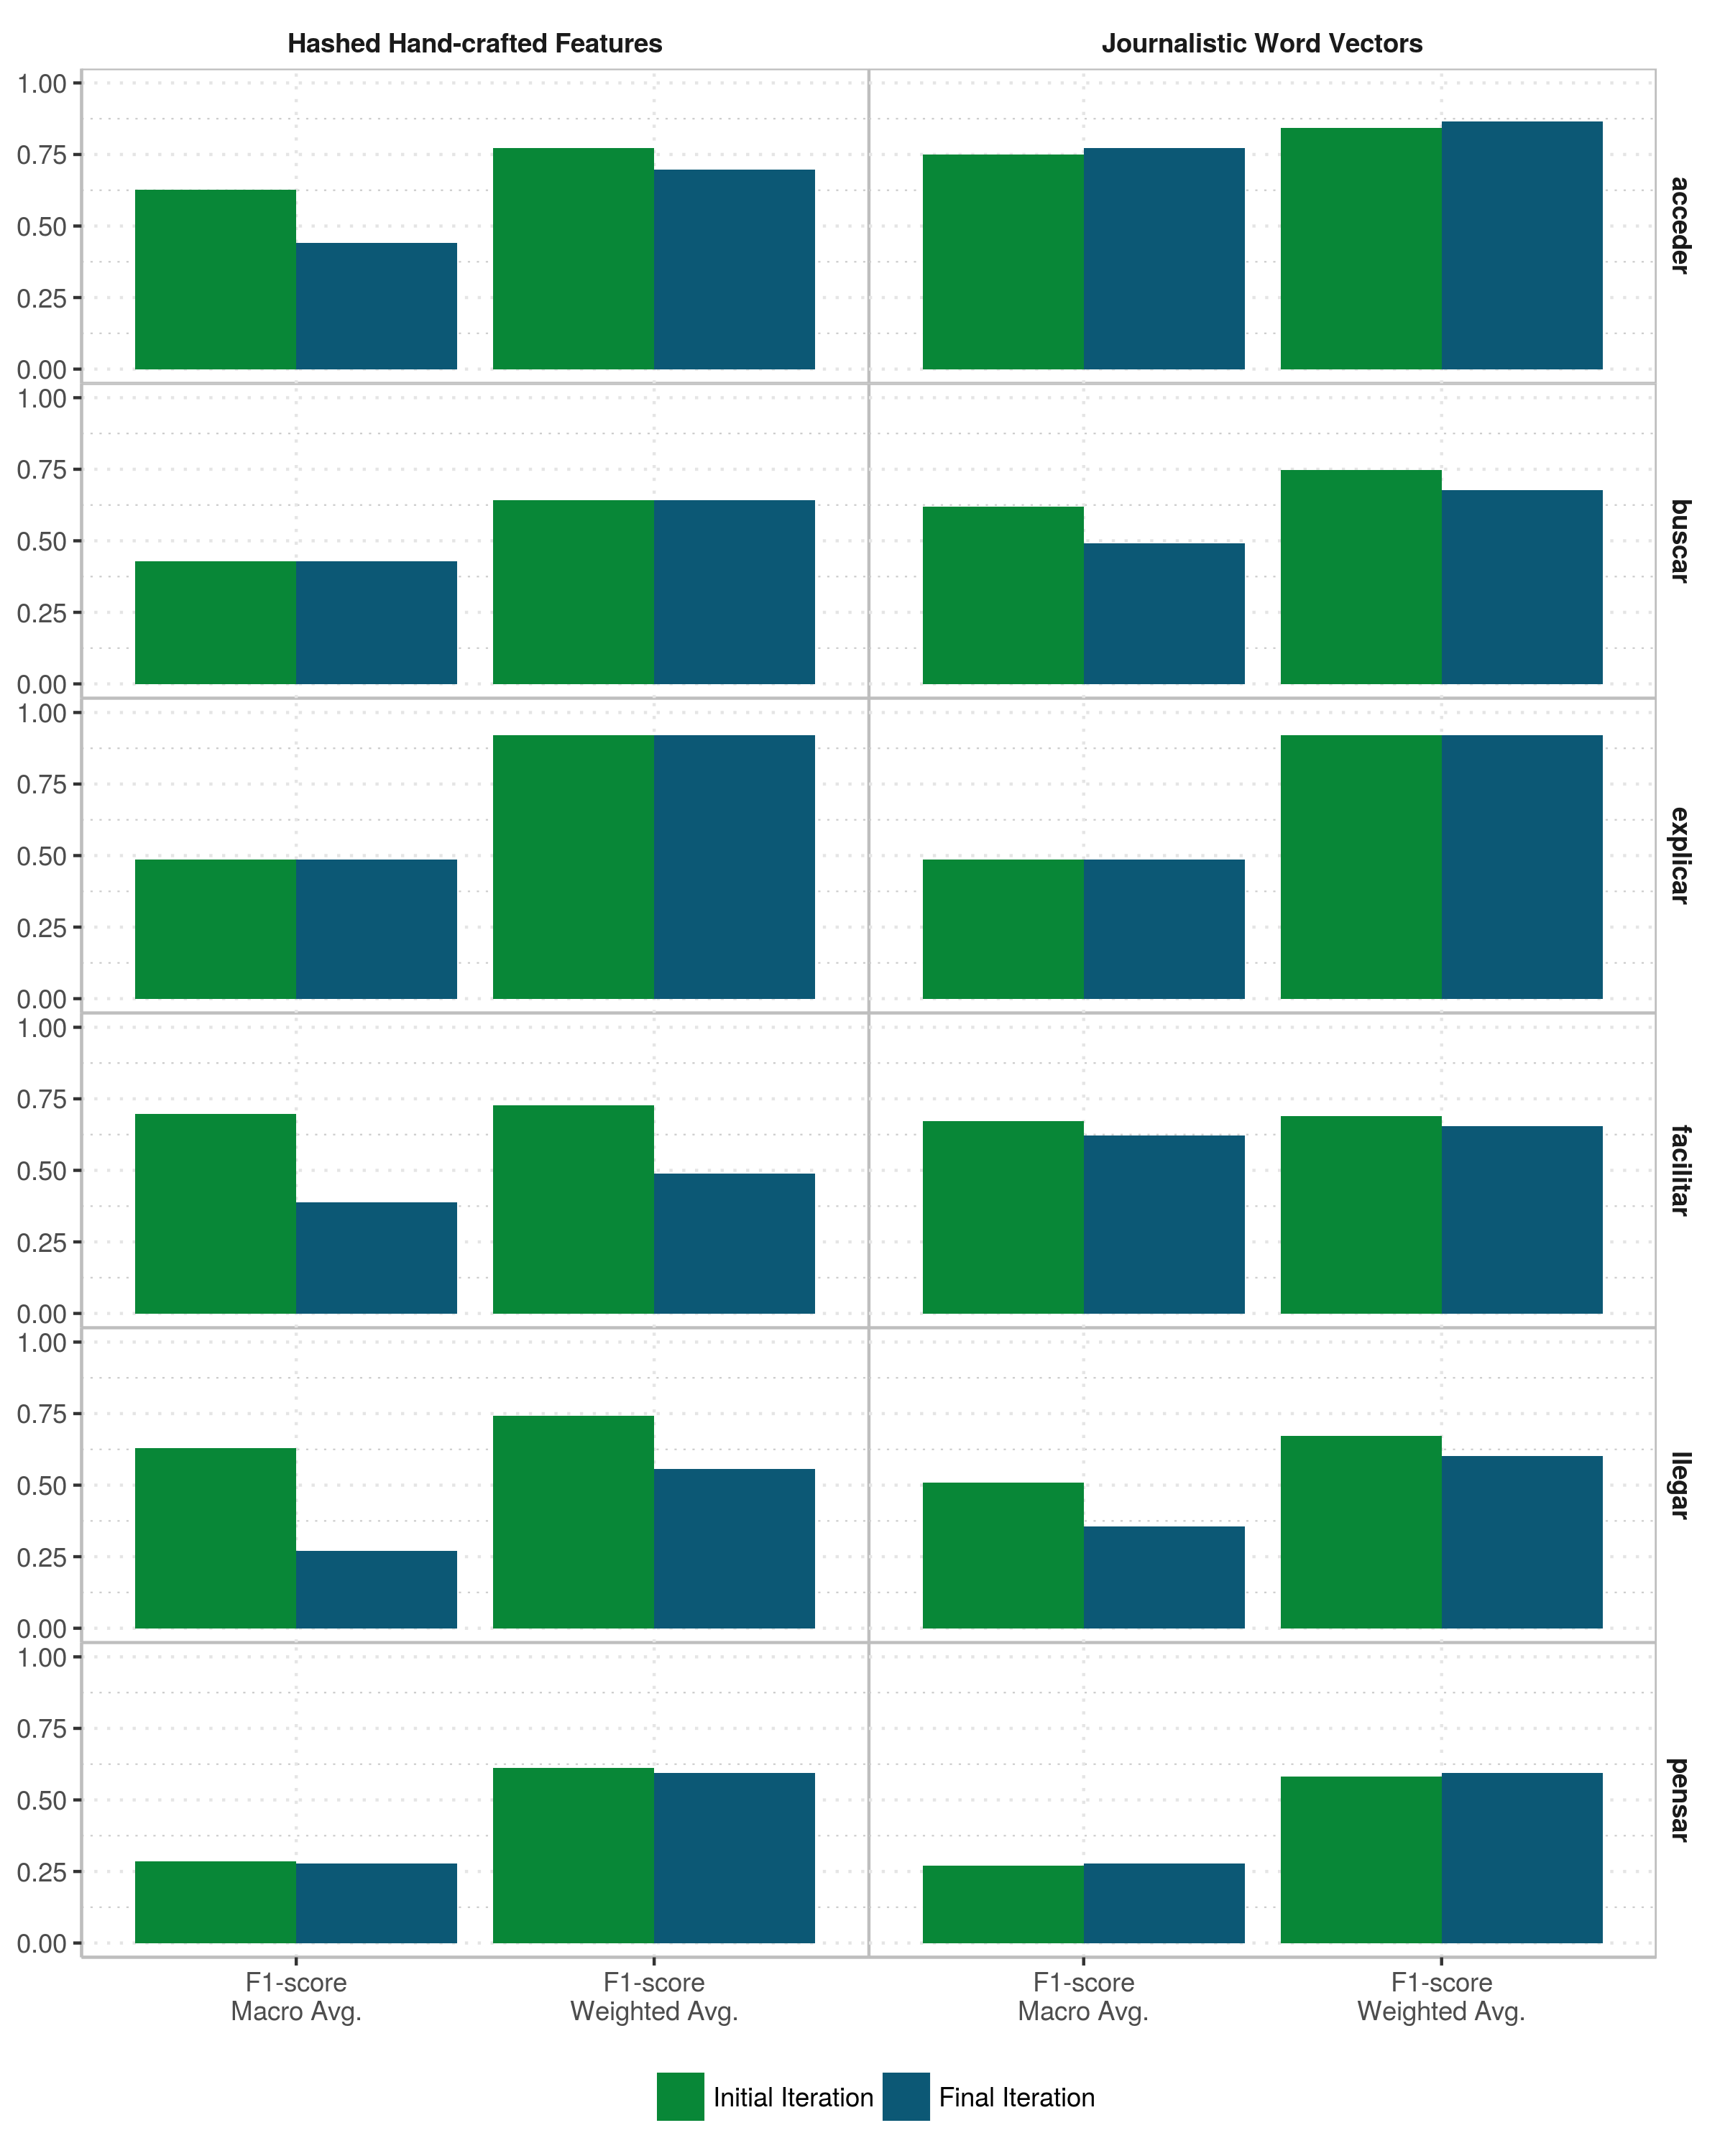
\includegraphics[height=.9\textheight,width=\textwidth,keepaspectratio]
    {plots/selflearning/test_results}
  \caption{Comparison of macro and weighted averaged F1-score before and after
  the self-learning algorithm's iterations}
  \label{fig:self-learning:test_performance}
\end{figure}

Figure \ref{fig:self-learning:test_performance} reports the performance results
on the test corpus before and after self-learning for each of the token lemmas
I presented in Section \ref{sec:self-learning:resources}. The plot is a bar
plot structured in the following way:

\begin{itemize}
  \item Each row shows the results for a token lemma: ``acceder'', ``buscar'',
    ``explicar'', ``facilitar'', ``llegar'', and ``pensar''.
  \item Each column stands for a feature representation: hand-crafted hashed
    features and journalistic word vectors.
  \item Each group of bars in each plot represents a metric: F1-score macro
    average and F1-score weighted average.
  \item Each bar plot in a different color inside a group represents the
    evaluation moment: initial iteration and final iteration.
  \item The bar plot represents the value of the metric.
\end{itemize}

As explained in Section \ref{sec:supervised:performance:metrics}, the weighted
average is useful to show the performance of the algorithm given the class
distribution (i.e. most frequent classes are more important in the final
result). On the other hand, the macro average is useful to see the performance
in less frequent classes. Then the spread between the macro and weighted
average shows how biased is the algorithm to the most frequent class.

Note that, as described in the previous chapter, word embeddings have worse
average performance than hand-crafted features. However, in two of the token
verbs shown here, word embeddings perform better than hand-crafted features, in
one of the verbs they perform at the same level and in three cases they perform
slightly worse. Actually, even if the average was different, the median was
very similar for word embeddings and hand-crafted features, so we can still
consider that these token verbs are representative of the population.

The figure shows that, except for two lemmas, hand-crafted features lose
performance after the self-learning algorithm ends. In none of the lemmas the
algorithm improves the performance over the original model without the new
data. For word embeddings the case is a little different, as in half of the
lemmas it does not lose performance, and it even improves in two of them. 

Comparing the loss in performance for the two different representations, the
drop is stronger for hand-crafted features, specially in the macro average.
From this results I can hypothesize that for hand-crafted features the
self-learning algorithm is more prone to add instances of the most frequent
class. This impacts in the performance of less frequent classes and is the
reason why the macro average drop in performance is much larger.

This drop in the performance measured by the macro average for word vectors is
not as pronounced as for hand-crafted features. Moreover, the general drop in
performance, in the cases when it happens, is not as big as for hand-crafted
features even if the latter have better performance for the initial iteration
(e.g. ``facilitar'', ``llegar'').

It can be concluded that, in general terms, word vectors work better than
hand-crafted features in this setting. This gives a strong indication of the
bias of the domain in the task. Hand-crafted features may have better
performance in the task with the original supervised dataset but they do not
generalize well to a bigger domain. In this case word embeddings provide a
better representation because, as we saw on the previous chapter, recalling
Hypothesis \ref{hyp:embeddings:2}, word embeddings have less tendency to
overfit a model. This is crucial in a setting like self-learning where new
examples are annotated automatically. In this setting, a better representation
makes the model adapt better to new data. I.e, hand-crafted features are
overfitting the model to the initial labeled dataset and that overfitting is
being transferred to the self-learning algorithm decisions regarding instances
to annotate automatically, producing a drift with a bias to the majority class.
Therefore, I can conclude that word vectors yield a better generalization of
the data for unseen examples.

The results do not show enough evidence to accept Hypothesis
\ref{hyp:self-learning:1}. In particular, hand-crafted features show evidence
to reject the Hypothesis as the general performance degrades after the
self-learning algorithm runs. Nevertheless, when word embeddings are integrated
in the setting, results are stronger to accept the Hypothesis, even if not
conclusive.

\subsection{Hypothesis \ref{hyp:self-learning:2}}\label{sec:self-learning:hyp:2}

The present section discusses the results I found regarding Hypothesis
\ref{hyp:self-learning:2}. The Hypothesis stated that the model trained after
each self-learning iteration, thus adding new data from unlabeled sources,
increased the average certainty to predict the class of new unseen examples.
Behind this hypothesis there is the assumption that the model, by adding new
unlabeled examples, can represent new examples better.

\begin{figure}[htb!]
  \centering
  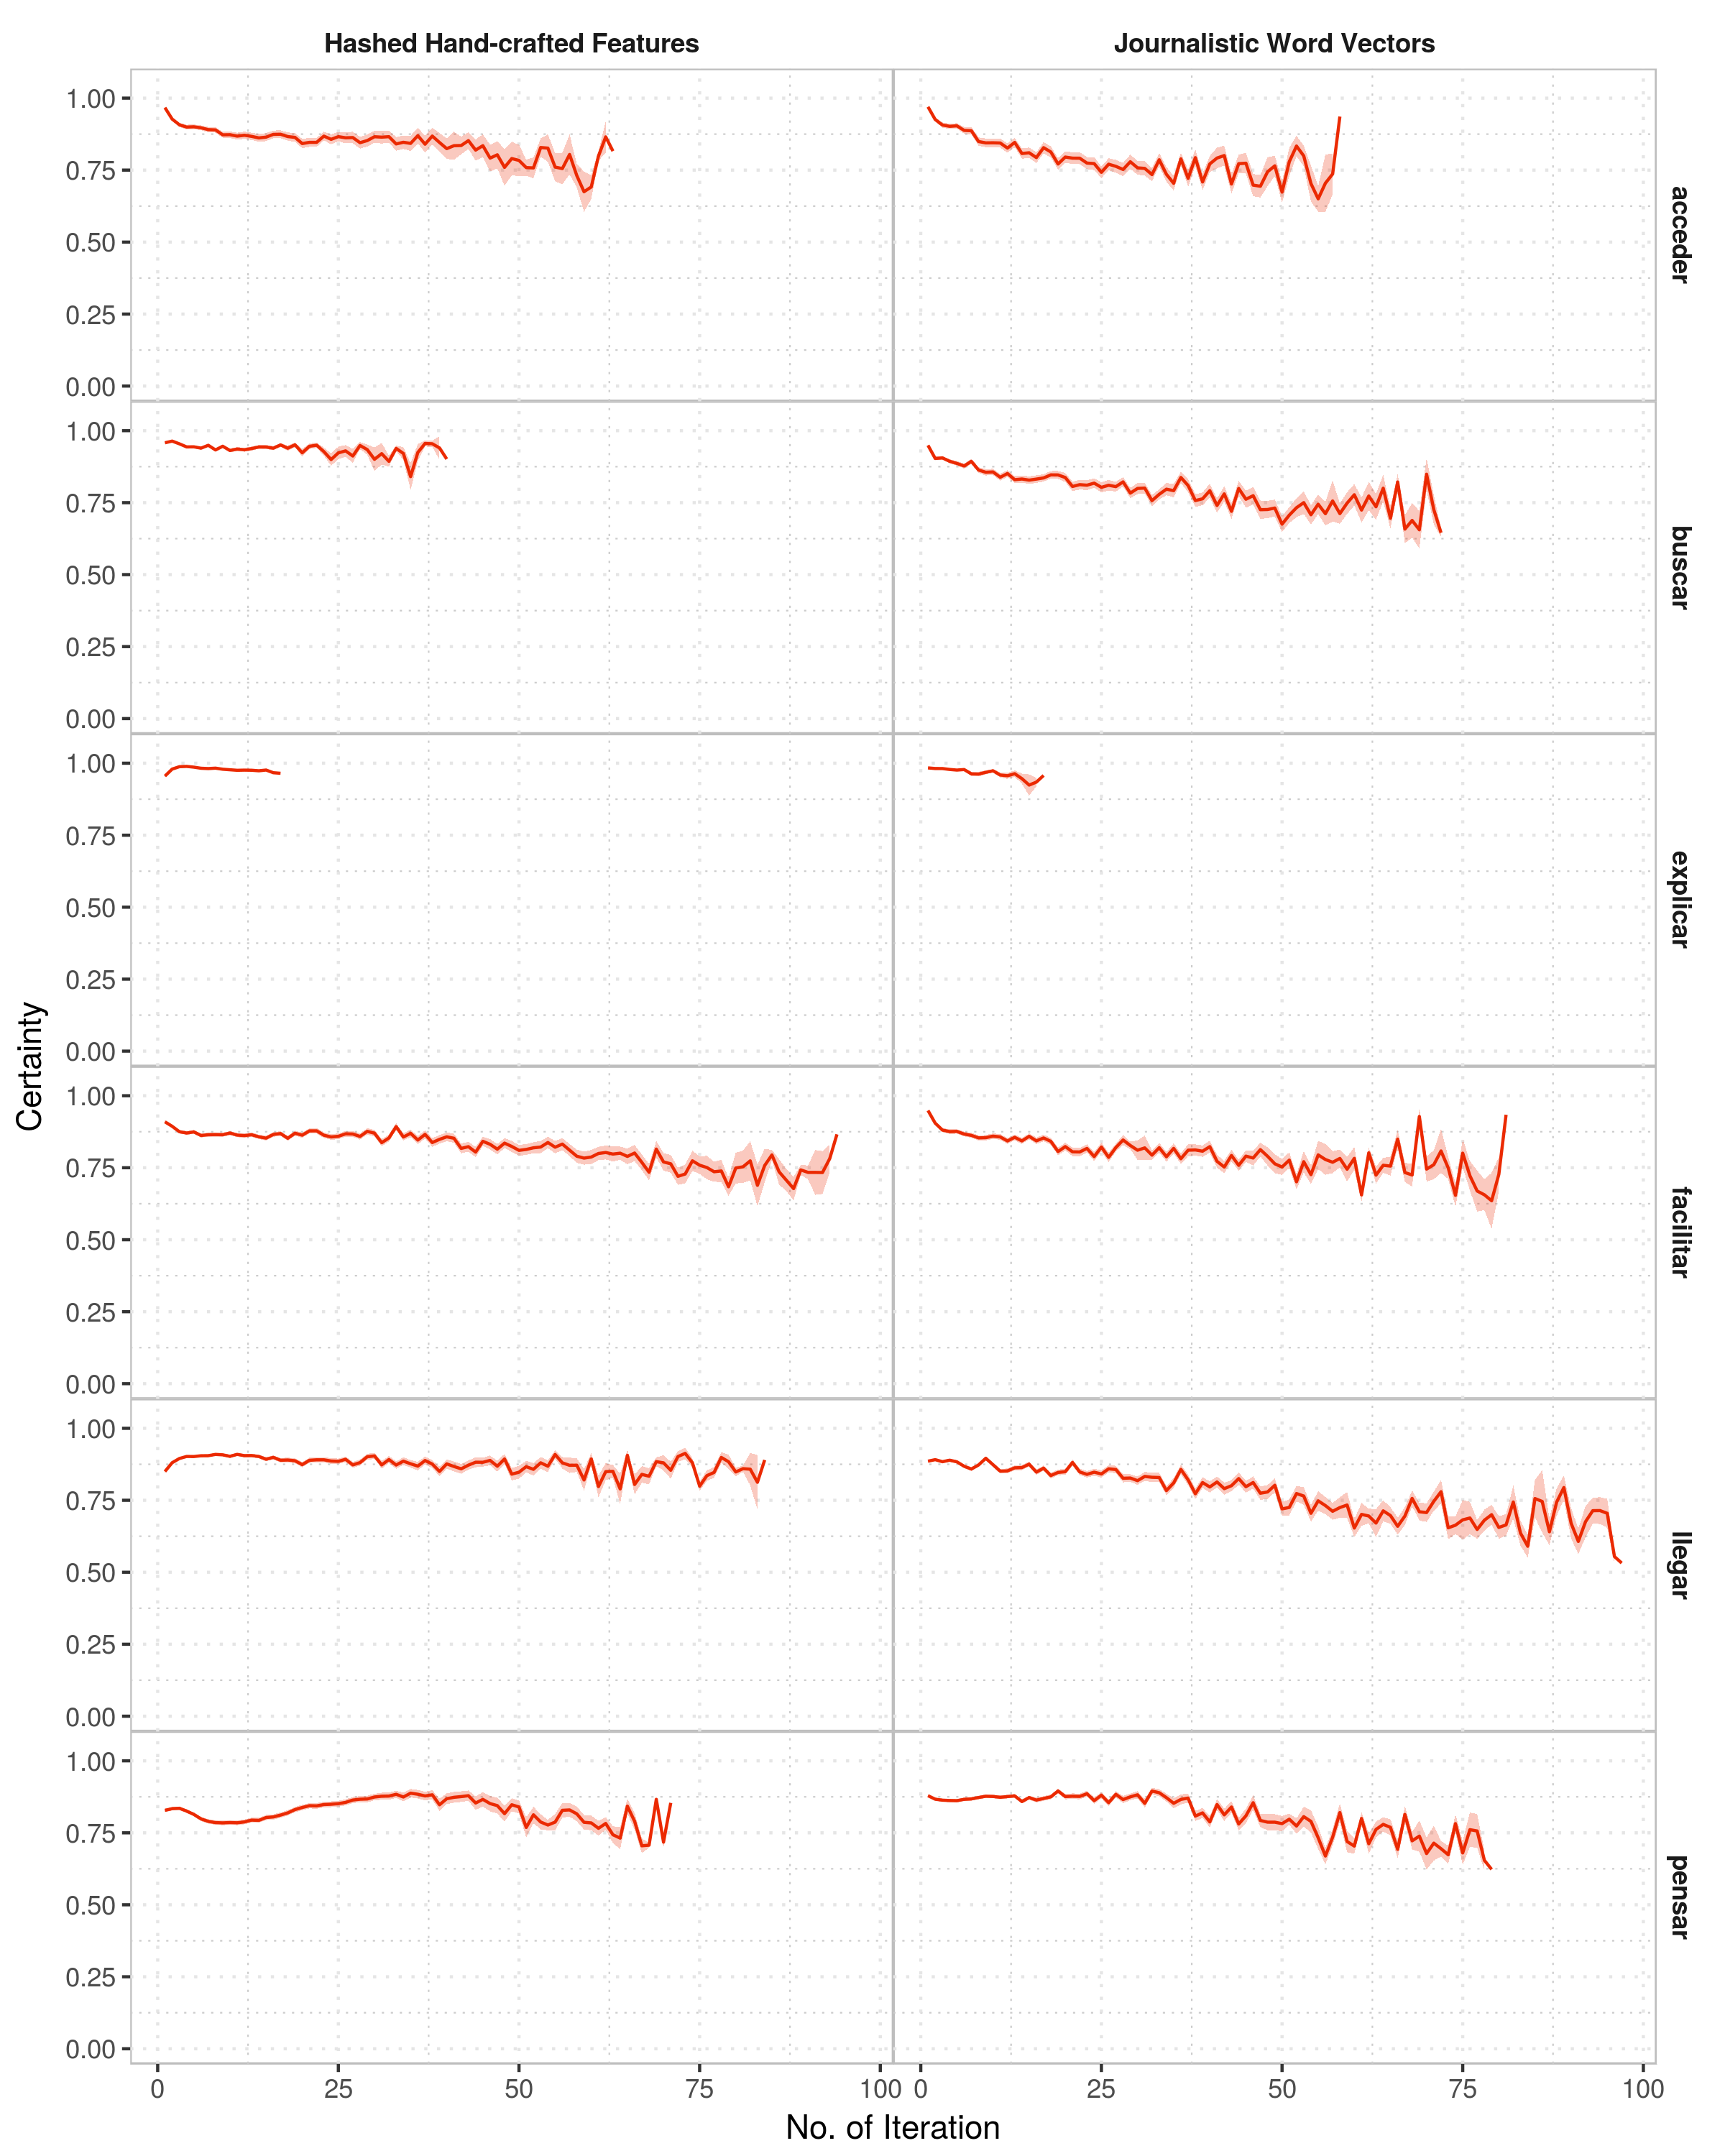
\includegraphics[height=.9\textheight,width=\textwidth,keepaspectratio]
    {plots/selflearning/certainty_progression}
  \caption{Average certainty to predict new classes for each self-learning
  iteration}
  \label{fig:self-learning:certainty}
\end{figure}

Figure \ref{fig:self-learning:certainty} shows the average certainty of the
model on new examples throughout the self-learning iterations. The data is
obtained running Experiment \ref{exp:self-learning:2}, which records the
predicted classes' certainty of the model for all the new examples from the
pool of unlabeled data. The metric to measure this is an unweighted average
described in Metric \ref{met:5}. The figure shows a line plot with the
following structure:

\begin{itemize}
  \item Each row shows the results for a token lemma: ``acceder'', ``buscar'',
    ``explicar'', ``facilitar'', ``llegar'', and ``pensar''.
  \item Each column stands for a feature representation: hand-crafted hashed
    features and journalistic word vectors.
  \item The x-coordinate axis represents the iteration number in the
    self-learning algorithm.
  \item The y-coordinate axis represents the raw count of features.
  \item The solid darker line represents the mean of certainty the mode has
    over the unlabeled data it is predicting.
  \item The shadowed area, which has a lighter color, represents the standard
    error of the mean of the certainty.
\end{itemize}

The plots I show are quite complex to follow and reason about. What is most
noticeable is that the certainty of the algorithm over the unseen examples is
less uniform as more iterations are added. In contrast to what I originally
assumed in Hypothesis \ref{hyp:self-learning:2}, the algorithm shows a lower
certainty over new examples. 

It is noticeable that hand-crafted features start with a certainty that is more
uniform through the initial iterations. Nonetheless as iterations go further,
certainty becomes more and more variable. Meanwhile, word vectors always show a
variable certainty over unseen examples. How certainty evolves through the
iterations in the self-learning algorithm gives us the idea that the model is
not converging, at least not in terms measured by certainty.

It is clear that the new examples add more uncertainty to the model, something
that becomes worse by adding more examples. Since the algorithm is drifting to
classify examples into the most frequent class, one would expect that the
certainty for the majority class is increased. However, what actually happens
is that the majority class accumulates many different examples. Most of these
examples are poorly characterized by the model, because most of their features
are unknown to the model. Thus, the classifier does not have a big certainty
over the majority class. Instead, it seems that many instances are classified
in that class only because the model does not have enough information to
classify them in any class, and it simply chooses the most probable one. In
sum, integrating more examples does not seem to increase the certainty because
they are not integrated in a smart manner, but relying only on the probability
of the majority class. Then, no new examples are added to minority classes (and
their certainty does not increase), and examples added to the majority class
only contribute to disperse the certainty.

\subsection{Hypothesis \ref{hyp:self-learning:3}}\label{sec:self-learning:hyp:3}

Hypothesis \ref{hyp:self-learning:3} is based on what I discussed in previous
chapters regarding the tendency of a model to overfit the training data. It
states that adding new unseen examples automatically through the self-learning
algorithm helps reducing the overfit of the model.

The Hypothesis is tested with the results reported by Experiment
\ref{exp:self-learning:3}. The experiment is similar to what I did in the
previous chapter to see the evolution of the {\em error due to variance} using
the learning curve of the model. The main difference lies in that in previous
chapters I needed to split the labeled dataset in order to simulate adding new
examples to a model. Thus, in previous chapters, new added examples were
actually labeled examples I left outside in the beginning.

Self-learning gives me the possibility to explore how real unseen examples
affect the tendency to overfit of a model measured by the learning curve
defined as Metric \ref{met:3} in Chapter \ref{chapter:supervised}.

There are however two possible views of the learning curve in this case. The
first approach is by plotting the curve in function of the iterations of the
algorithm. The second approach is to plot the curve in function of the number
of examples used for training.

The first approach is more focused on how the self-learning algorithm works
rather on how the model evolves. In each iteration the number of examples added
can be high or low. As I did not limit the number of new examples to add, there
is no certain way of telling how many the algorithm is adding for each
iteration. What the results show in this case is rather how the added examples
affect the model in that iteration. The second approach is more analogous to
what is shown in previous chapters, as the plot is done based on the number of
examples of the training dataset rather than the iteration they were added.

Both views are useful on their own ways, nevertheless for comparison with the
previous methods I opted for analyzing the second approach as it is closer to
what I already discussed for supervised and word embeddings approaches before.

\begin{figure}[htb!]
  \centering
  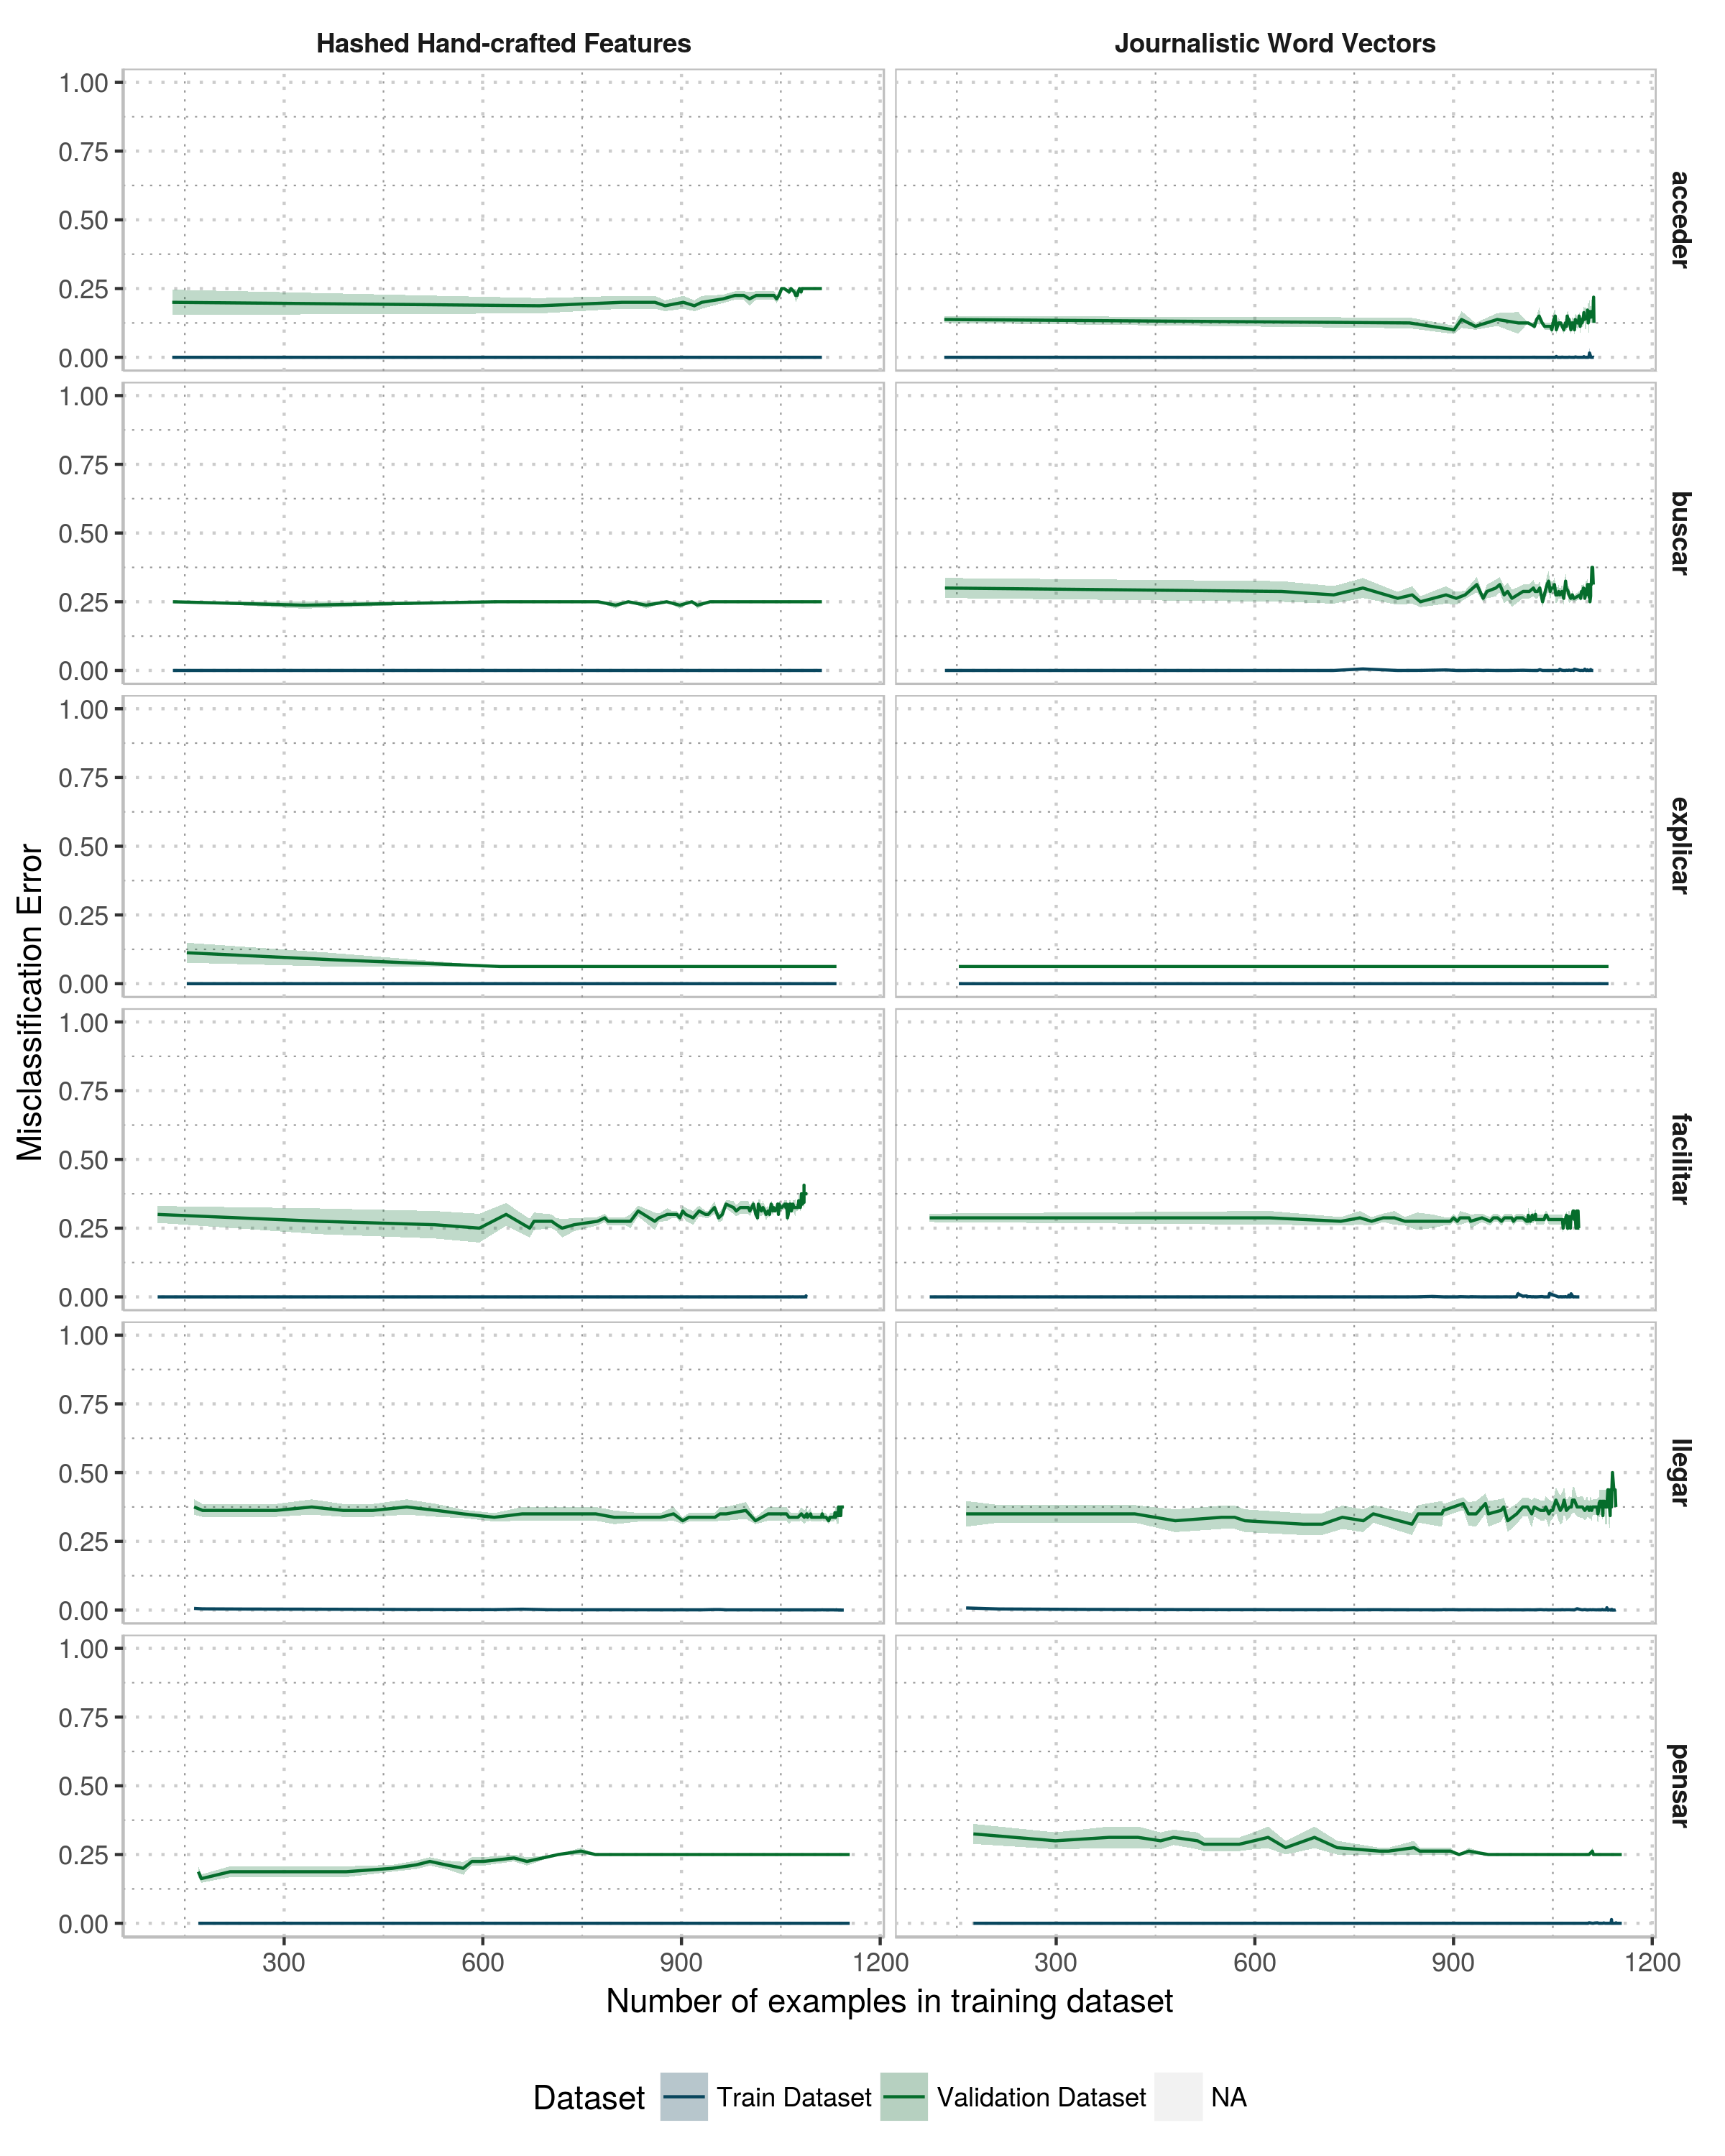
\includegraphics[height=.9\textheight,width=\textwidth,keepaspectratio]
    {plots/selflearning/overfit_measure_per_examples}
  \caption{Learning curve as a function of the number of examples added by the
  self-learning algorithm}
  \label{fig:self-learning:overfit}
\end{figure}

Figure \ref{fig:self-learning:overfit} shows the learning curve plot as a
function of the number of examples of the training dataset. The structure of
the learning curve plot is as follows:

\begin{itemize}
  \item Each row shows the results for a token lemma: ``acceder'', ``buscar'',
    ``explicar'', ``facilitar'', ``llegar'', and ``pensar''.
  \item Each column stands for a feature representation: hand-crafted hashed
    features and journalistic word vectors.
  \item The x-coordinate axis represents the number of examples in the
    self-learning algorithm.
  \item There are two colors representing the datasets: train and validation
    (in this case is the validation set).
  \item The solid darker lines represent the mean of misclassification error
    trough the different iterations of the datasets over all the models.
  \item The shadowed area, which have a lighter color, represent the standard
    error of the mean of the misclassification error.
\end{itemize}

Recall I am limiting my unlabeled pool of data to 1000 unannotated examples and
that is why none of the plots go beyond 1150 examples total (that is the
original supervised dataset plus the automatically annotated examples).

A first look into the graphics shows that the misclassification error drops a
little after the first set of automatically annotated examples is added. This
is more or less uniform for all the lemmas for the first increments. If I take
into consideration that these examples are added in the first iterations, it is
interesting to see that the first iterations are the ones adding up to improve
the generalization of the model. This happens regardless of the representation
used.

It is also interesting to see that in general terms the shadowed area, which is
the standard error of the mean for the misclassification error, becomes
narrower the more examples are added. This means the model has less variance
over the validation dataset. This is an indication of the model reducing the
error due to variance, which is one of our indicators of reduced overfitting.

Besides that, it is striking how the error in the validation dataset starts to
become highly irregular for every new example added. This happens in most of
the cases for the examples added in later iterations. This can be due to the
fact that in the final iterations of the algorithm, the tolerated error level
in the validation dataset is bigger. Indeed, the tolerated error in the
validation dataset is slowly increased by the method as iterations go, and
until it reaches the stopping threshold. This is specially relevant for the
case of word embeddings. It may require a further analysis left for future work
for now.

This tendency could be further explore and systematized to the point that it
can be used as a stopping criterion for the algorithm. Indeed, the difference
in validation and training error over the iterations could be a good stopping
criterion.

\subsection{Hypothesis \ref{hyp:self-learning:4}}\label{sec:self-learning:hyp:4}

Hypothesis \ref{hyp:self-learning:4} is based on what I talked about previously
regarding model coverage. To measure the coverage I do so by counting the
features the model recognizes. For hand-crafted features this means all the
features obtained from the training data (which includes words, tokens,
part-of-speech, etc. as explained in Section \ref{sec:supervised:features}).
For the case of word embeddings, the features are the words surrounding the
verb to disambiguate and the position relative to that verb. There is more than
one way to measure the coverage of a model by its features. Hypothesis
\ref{hyp:self-learning:4} is interested in showing that the model increases
it is number of features by adding new examples so I get the raw count of the
total number of features the model has in the training dataset over the
self-learning iterations.

\begin{figure}[htb!]
  \centering
  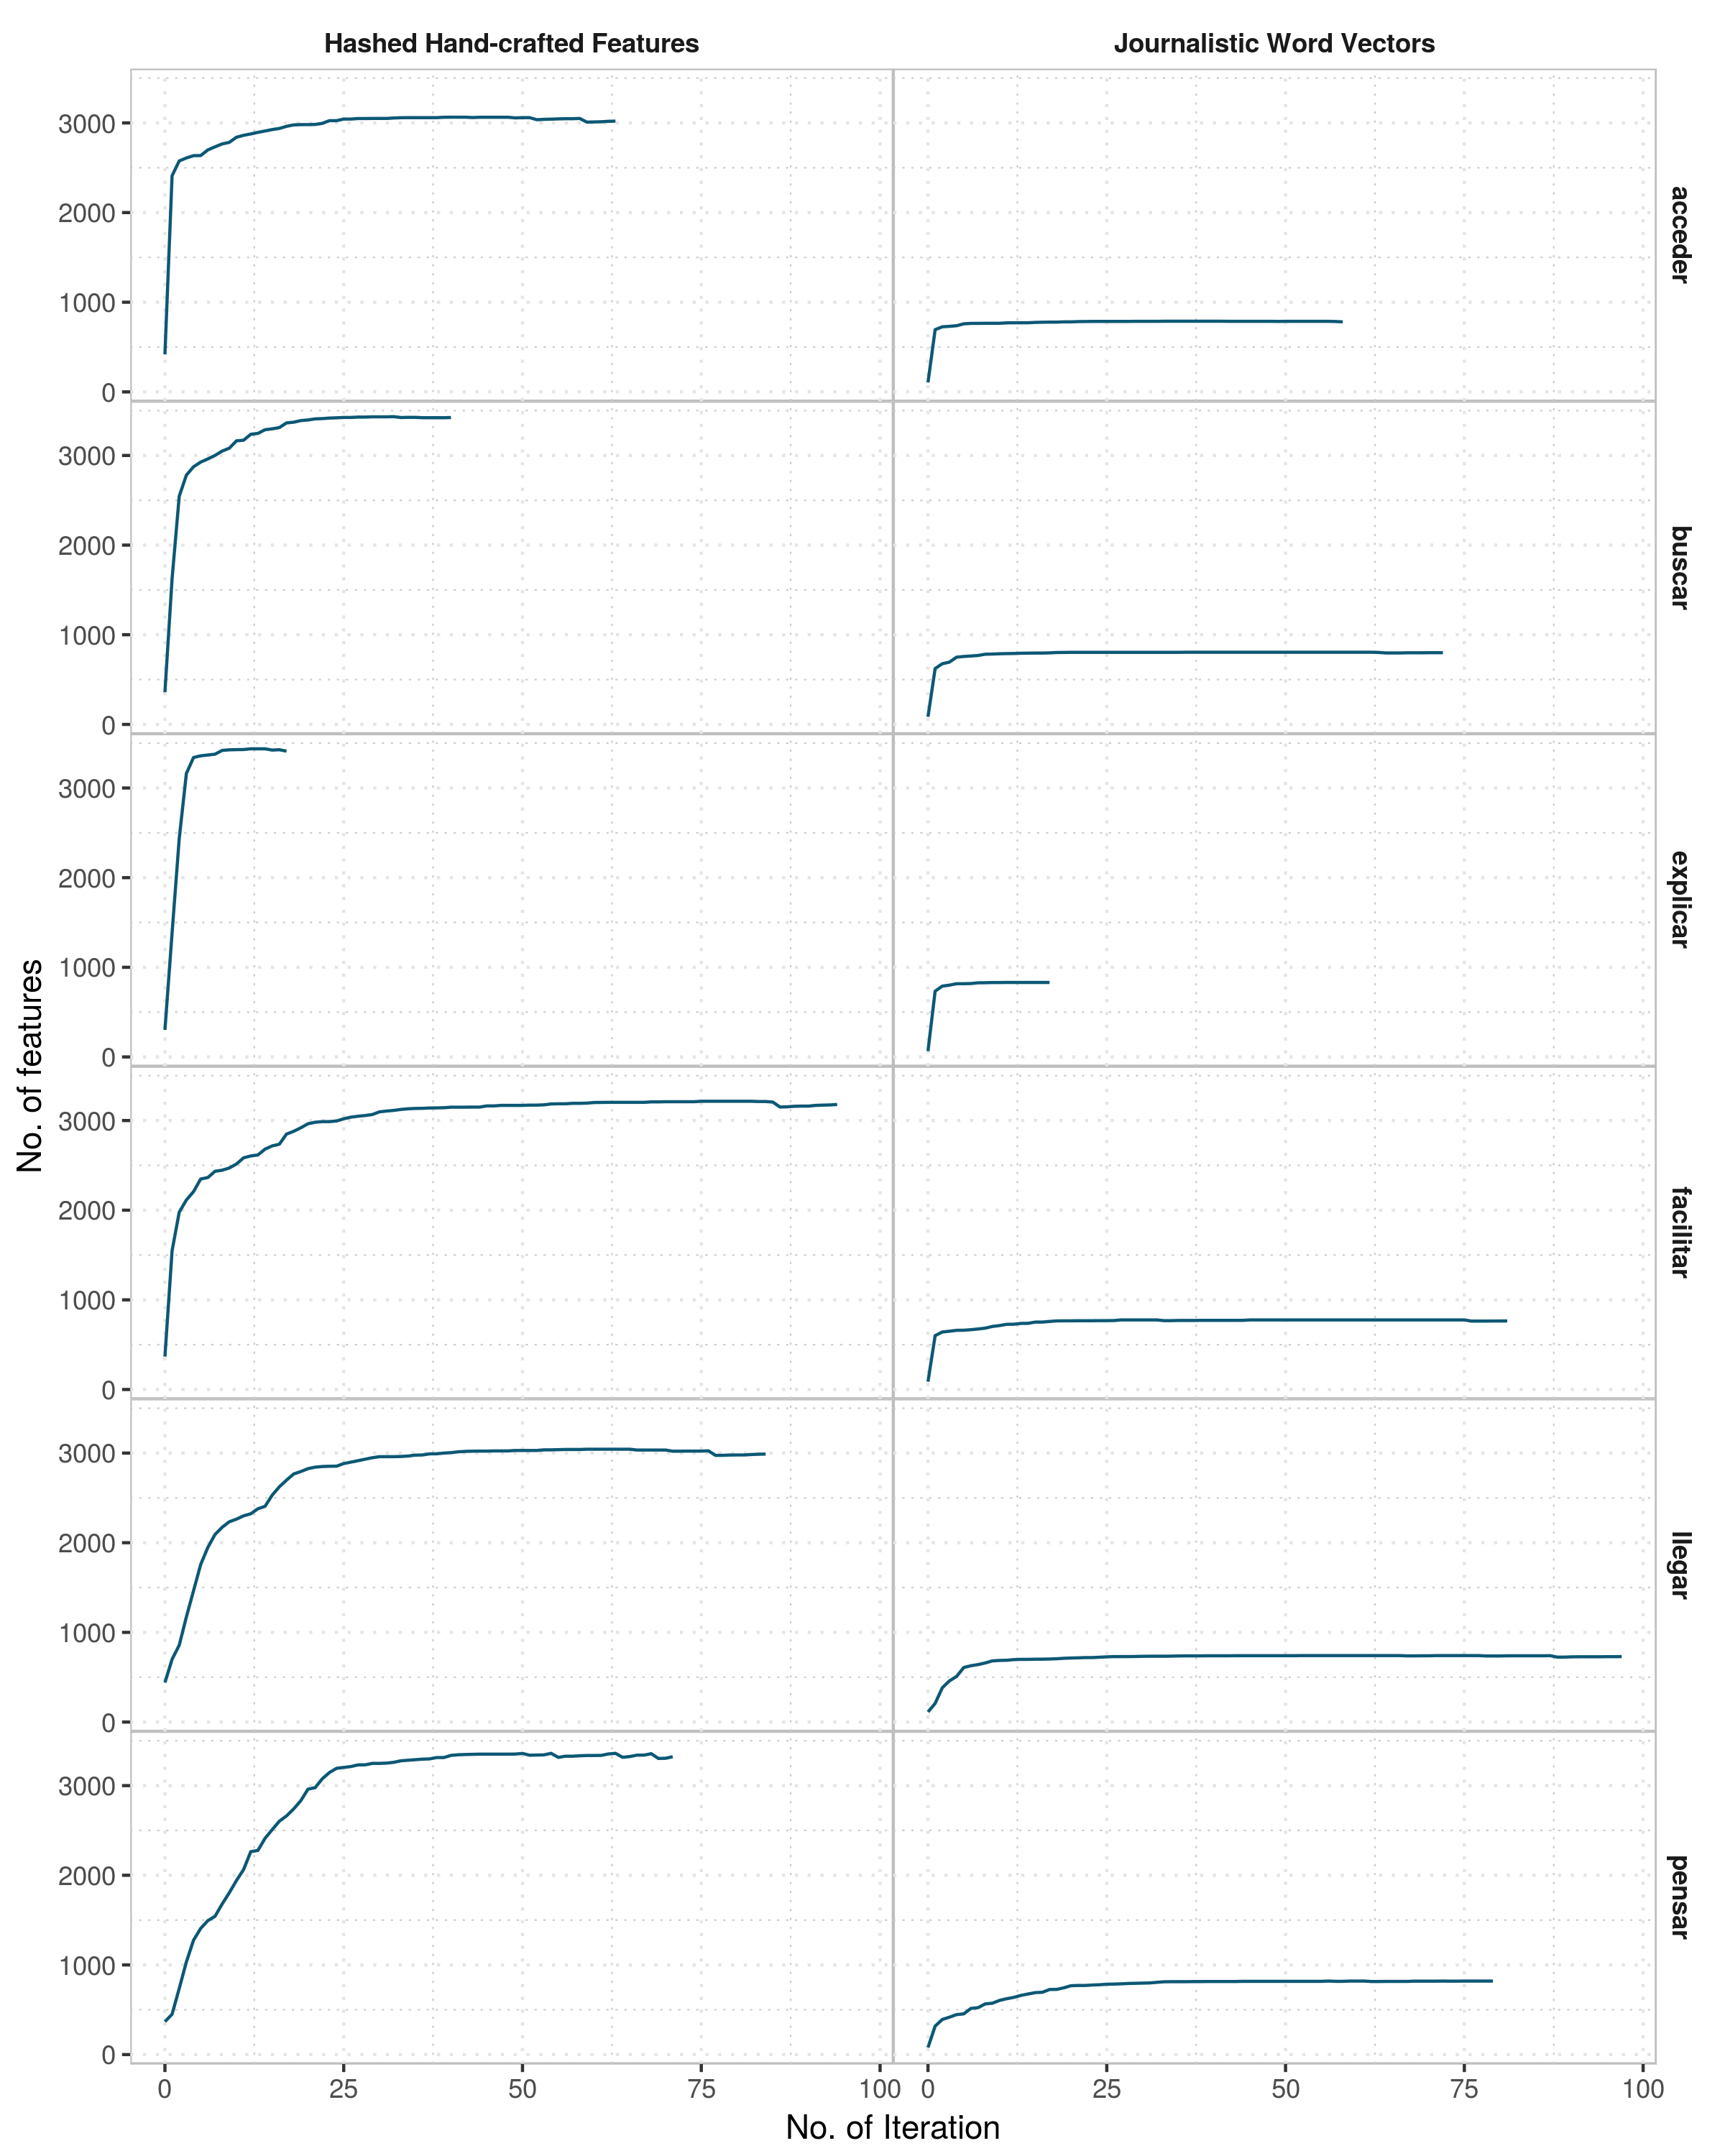
\includegraphics[height=.9\textheight,width=\textwidth,keepaspectratio]
    {plots/selflearning/features_growth_total}
  \caption{Features' growth in the model across self-learning iterations}
  \label{fig:self-learning:features_growth_total}
\end{figure}

Figure \ref{fig:self-learning:features_growth_total} reports the features'
growth of the model across the self-learning iterations. That is the total
number of unique features up to that iteration obtained both from the original
supervised dataset and the automatically annotated data. The figure shows a
line plot with the following structure:

\begin{itemize}
  \item Each row shows the results for a token lemma: ``acceder'', ``buscar'',
    ``explicar'', ``facilitar'', ``llegar'', and ``pensar''.
  \item Each column stands for a feature representation: hand-crafted hashed
    features and journalistic word vectors.
  \item The x-coordinate axis represents the iteration number in the
    self-learning algorithm.
  \item The y-coordinate axis represents the raw count of unique features.
\end{itemize}

From the figure it is visually striking that most of the new features are
acquired in the first iterations of the self-learning algorithm. After that the
number of features stales. This is an indication of the algorithm adding lot of
examples in the first iterations while almost none in the following ones.

It is interesting to note the difference between hand-crafted features and word
vectors. It is natural because of what I explained previously regarding what is
that I am considering as features for each type of representation. The pool of
features for the word embeddings model is much smaller than for hand-crafted
features. Regardless of the scale, there is a shared pattern for both
representations regarding the way the features in the models grow.

These results show that the model effectively increases the features associated
to it, which is stated by Hypothesis \ref{hyp:self-learning:4}. The hypothesis
is accepted in that way. However, this is not necessarily an increase in the
coverage of the model as I will show in further sections.

\subsection{Hypothesis \ref{hyp:self-learning:5}}\label{sec:self-learning:hyp:5}

In this section I discuss the results regarding Hypothesis
\ref{hyp:self-learning:5}. This hypothesis together with the following two in
this chapter are expected to be false (in contrast to the previous ones).
Hypothesis \ref{hyp:self-learning:5} states that self-learning helps improving
the performance of the model on each class uniformly.

To test this hypothesis I work on the results of Experiment
\ref{exp:self-learning:1} again. Remember that in that experiment the idea is
to evaluate the model over the held-out test dataset before and after running
the self-learning iterations. However, this time, instead of reporting the
averages defined in Metric \ref{met:1}, I show the F1-score for the most
frequent, second most frequent and, in some cases, third most frequent class of
the lemma. I do this because these are the classes of the token lemmas that
were not filtered out in the preprocessing of the corpus. From the 6 token
lemmas, 4 of them have only two senses with instances in the labeled dataset
(``acceder'', ``buscar'', ``explicar'', and ``facilitar''), and only 2 of them
have 3 senses with instances in the dataset (``llegar'' and ``pensar'').

\begin{figure}[htb!]
  \centering
  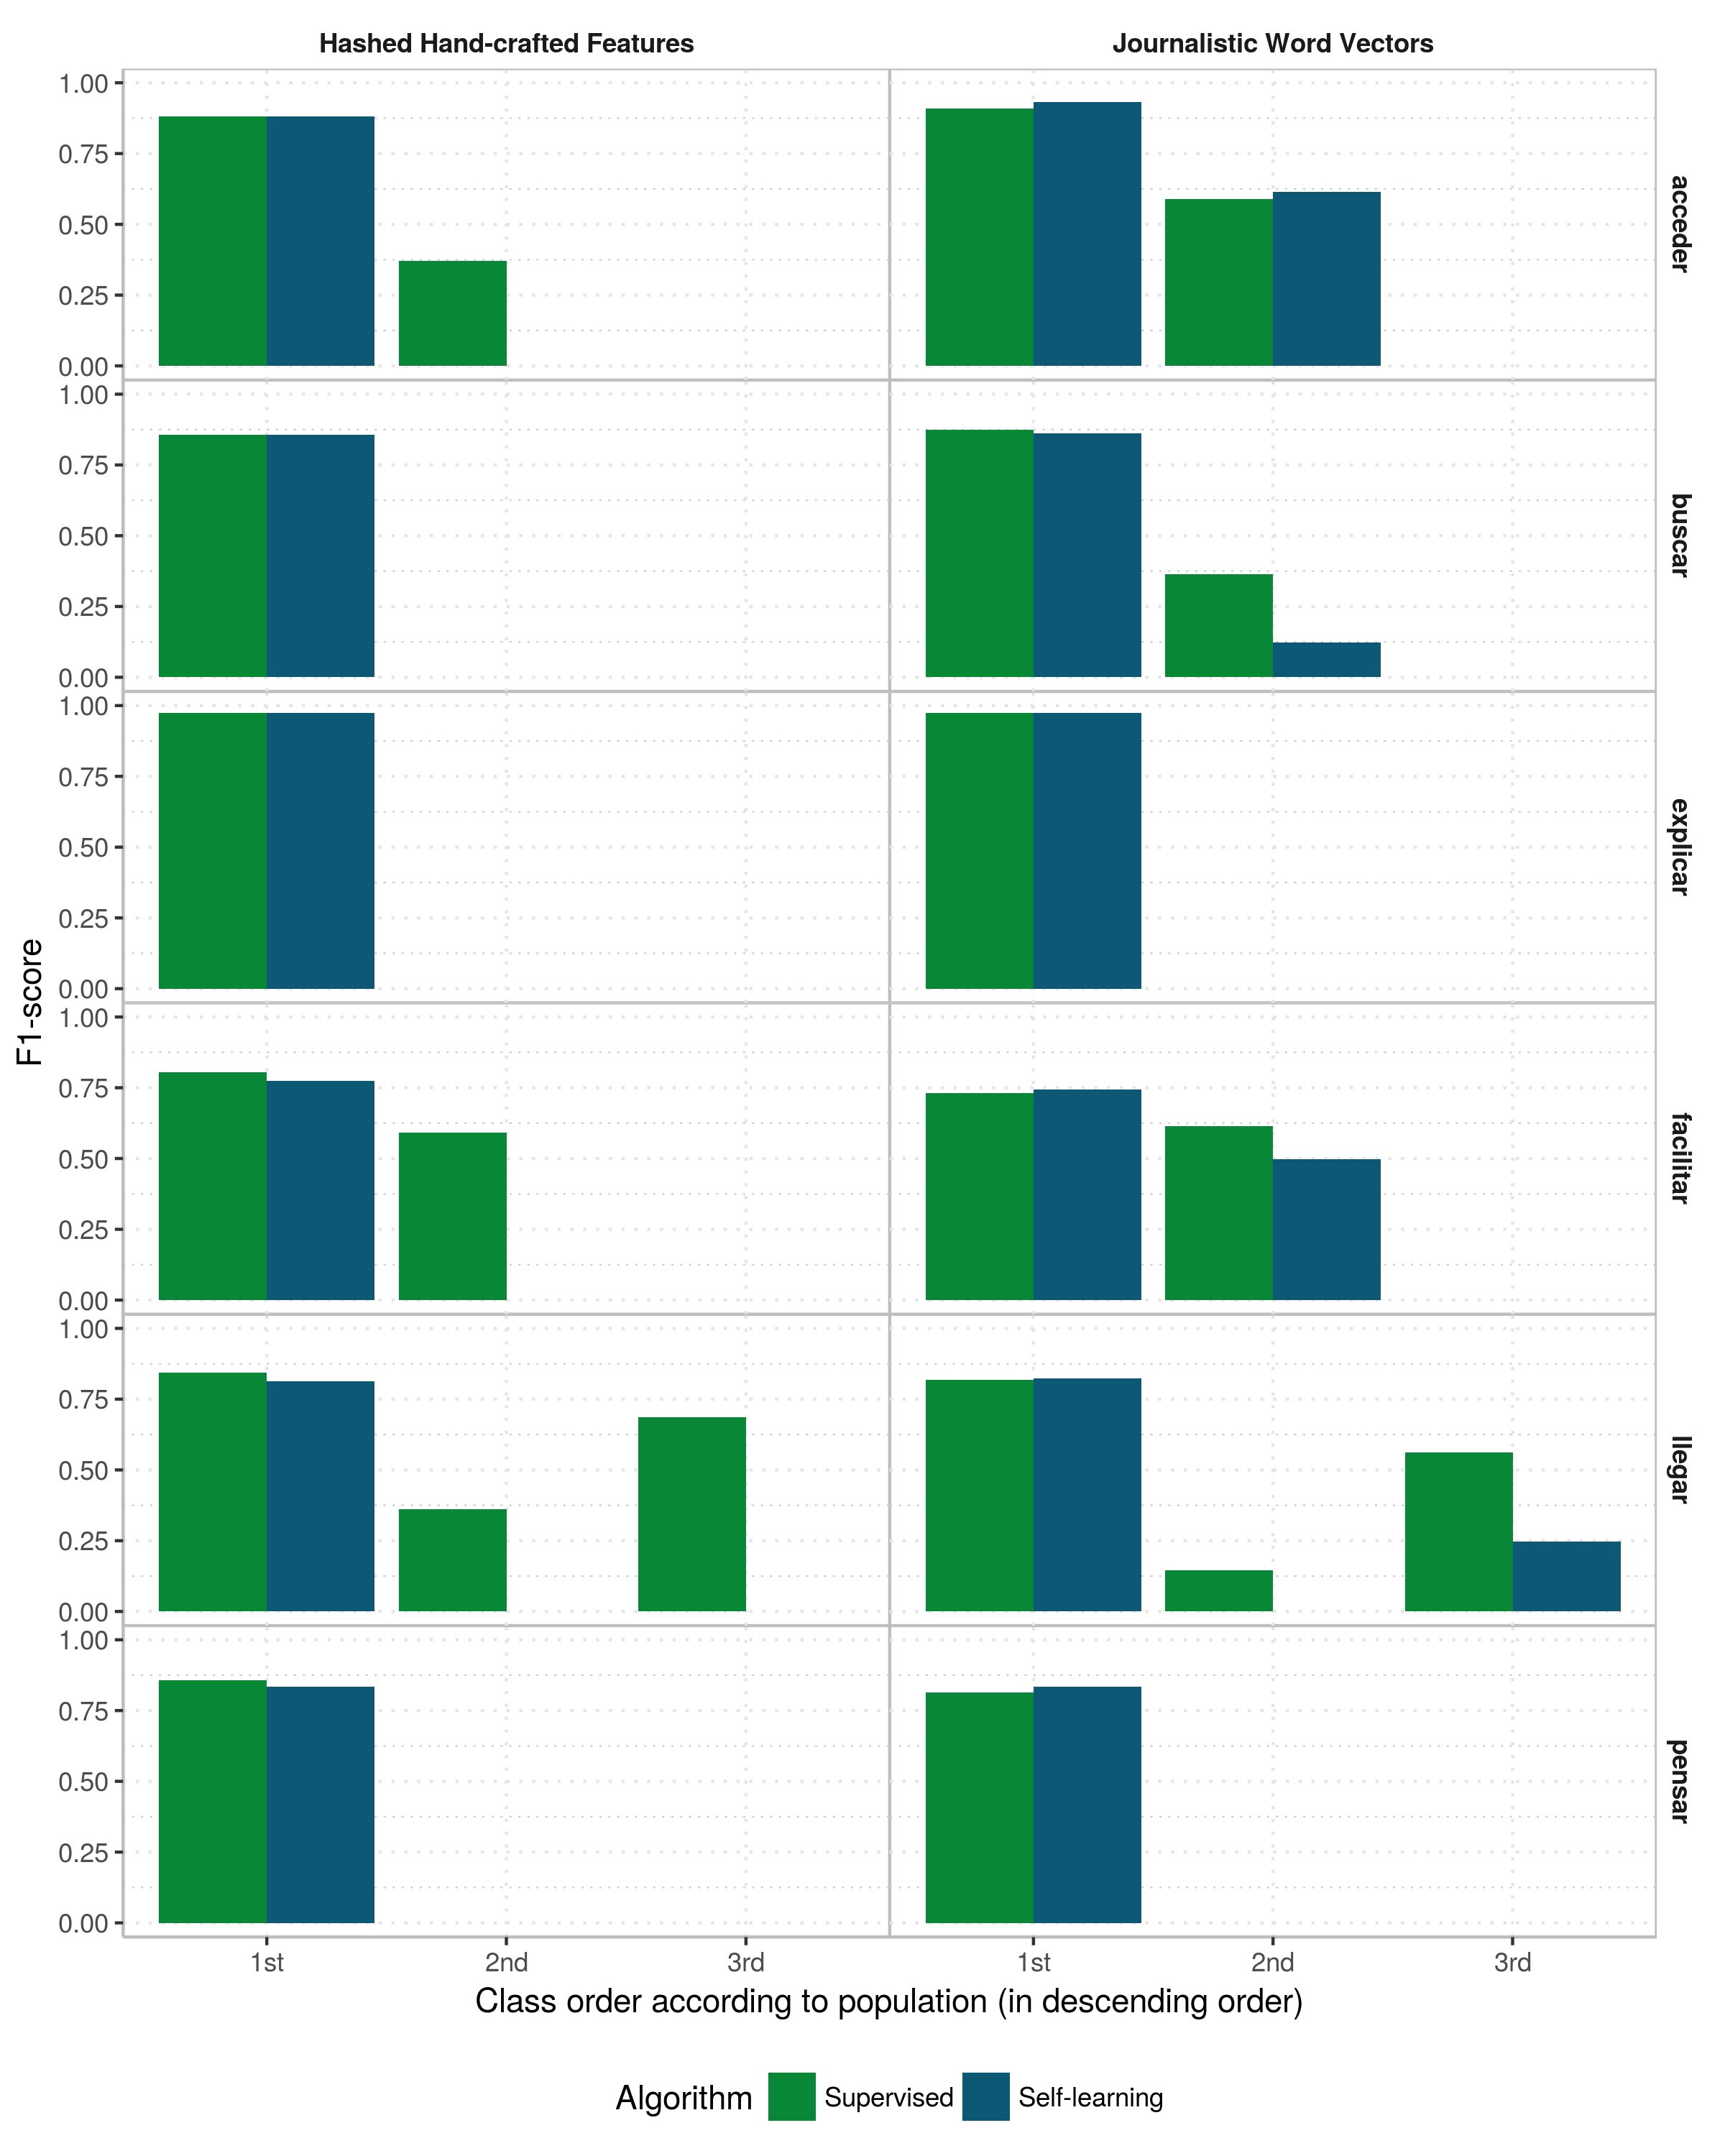
\includegraphics[height=.9\textheight,width=\textwidth,keepaspectratio]
    {plots/selflearning/per_sense_fscore}
  \caption{Comparison of F1-score for each class before and after the
  self-learning algorithm's iterations for the token lemmas}
  \label{fig:self-learning:per_class_performance}
\end{figure}

Figure \ref{fig:self-learning:per_class_performance} reports the performance
results on the test corpus for supervised (i.e. before the self-learning
iteration starts) and self-learning algorithms for each class (i.e. sense) of
each of the token lemmas I presented in Section
\ref{sec:self-learning:resources}. The plot is a bar plot structured in the
following way:

\begin{itemize}
  \item Each row shows the results for a token lemma: ``acceder'', ``buscar'',
    ``explicar'', ``facilitar'', ``llegar'', and ``pensar''.
  \item Each column stands for a feature representation: hand-crafted hashed
    features and journalistic word vectors.
  \item Each group of bars in each plot represents the class (i.e. sense) for
    that lemma. These are ordered according to number of occurrences of the
    class in the dataset.
  \item Each bar plot in a different color inside a group represents the
    algorithm: supervised (i.e. evaluation moment of the initial iteration),
    self-learning (i.e. evaluation moment of the final iteration after
    self-learning finishes).
  \item The height of the bar represents the value of the F1-score per each
    class.
\end{itemize}

Recall again that only the last two rows of the graphics have lemmas with 3
senses (i.e. ``llegar'' and ``pensar''). The first four lemmas can at most show
results for two senses.

From the figure it is clear that the self-learning algorithm is affecting
negatively the performance of all the classes that are not the most frequent
class. The only lemma in which there is a slight improvement in performance for
a class that is not the most frequent one is the lemma ``acceder'' and only
does so with the word embeddings representation.

This plot gives more information based on each class rather than obscuring
everything into an averaged metric. From it I can see that even though word
embeddings may have less performance in classes other than the most frequent,
the self-learning algorithm does not affect it as much as it does for
hand-crafted features. With hand-crafted features the F1-score directly drops
to zero for all classes other than the most frequent one. This is clearly a
sign of divergence to the most frequent class when new examples are added by
the self-learning algorithm.

The results are clear in this case and it is safe to reject Hypothesis
\ref{hyp:self-learning:5} as I originally thought.

\subsection{Hypothesis \ref{hyp:self-learning:6}}\label{sec:self-learning:hyp:6}

The next Hypothesis to test is \ref{hyp:self-learning:6}. This is an extension
of the explanation for the previous hypothesis as it states that the
representativity of each class in the dataset is maintained through all the
iterations of the self-learning algorithm. By representativity I mean the
number of classes as a proportion of the whole training dataset. This
Hypothesis is expected to be false and is a result of the self-learning
algorithm tendency to classify every new instance as the most frequent class.

Experiment \ref{exp:self-learning:5} is used in this section to report the
results of the self-learning algorithm with respect to the representativity of
each class through iterations. The experiment records the distribution of the
classes in the training dataset in each iteration. The metric to measure this
is the proportional count of occurrences each class, with respect to the whole
data available

To visualize these results I focus on two aspects I find relevant when
considering the hypothesis. First is the proportional count of number of
instances per class along the iterations of the algorithm. Second I want to
show how many examples of each class are added in each of the iterations of the
algorithm as a proportion of all the examples added in that iteration.

\subsubsection{Classes' population distribution across iterations}

\begin{figure}[htb!]
  \centering
  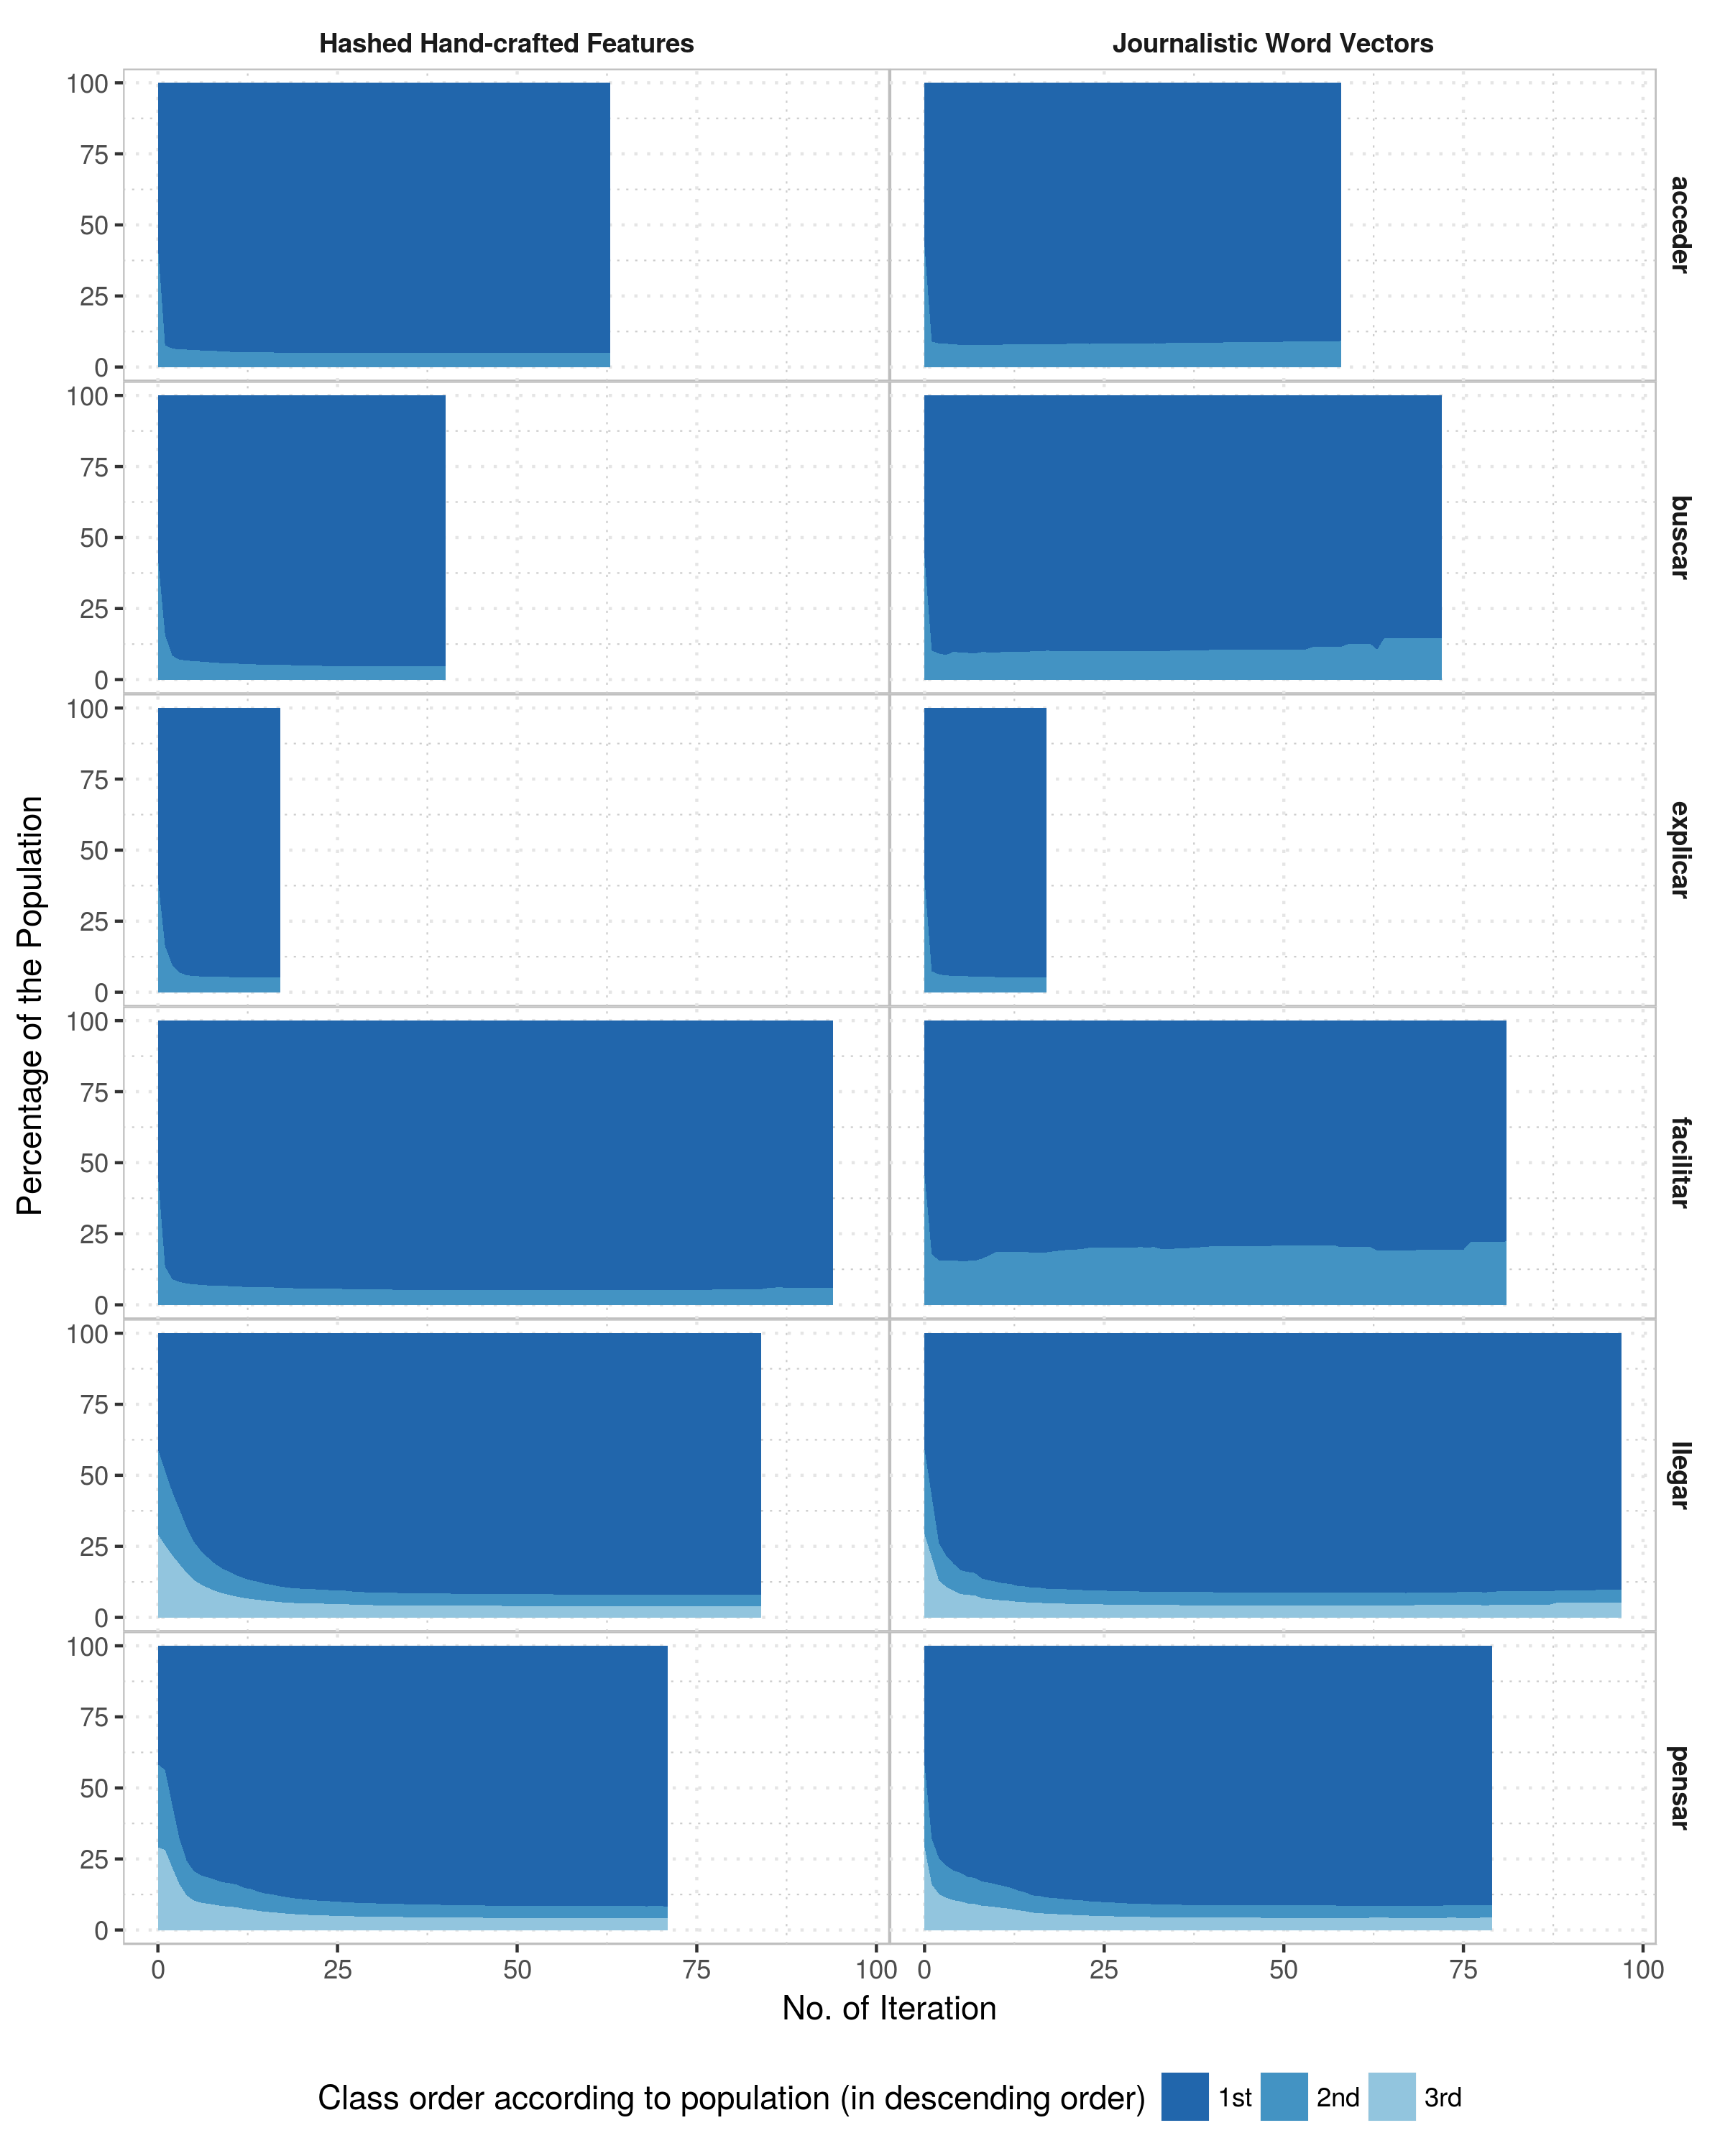
\includegraphics[height=.9\textheight,width=\textwidth,keepaspectratio]
    {plots/selflearning/population_distribution}
  \caption{Distribution of the classes' population across self-learning
  algorithm's iteration as a proportion of the whole training dataset}
  \label{fig:self-learning:population_distribution}
\end{figure}

Figure \ref{fig:self-learning:population_distribution} showcases the
distribution of the population of the classes across the self-learning
iterations of the algorithm. Each class's population is represented as the
proportion of the total number of examples in the training dataset for that
iteration. The plot is a stacked area plot that follows this structure:

\begin{itemize}
  \item Each row shows the results for a token lemma: ``acceder'', ``buscar'',
    ``explicar'', ``facilitar'', ``llegar'', and ``pensar''.
  \item Each column stands for a feature representation: hand-crafted hashed
    features and journalistic word vectors.
  \item The x-coordinate represents the iteration in the self-learning
    algorithm.
  \item The y-coordinate represents the percentage of population.
  \item Each area of a different color represents the proportion of examples
    for each of the classes in the dataset. The classes again are ordered
    according to number of examples in the original supervised dataset.
\end{itemize}

Figure \ref{fig:self-learning:population_distribution} shows the clear
predominance of the most frequent class in the self-learning algorithm. For
some lemmas the progress is a little less steep, for others the algorithm
starts to classify most instances into the most frequent class from the
beginning.

Recall that the number of classes is very unbalanced in the original manually
annotated corpus. To make this less of a problem, the corpus I have been using
in all these experiments has minority classes oversampled so that the number of
examples per class is more uniformly distributed. Even so, the models still
diverge quickly to the majority class.

From this figure I have evidence to reject the hypothesis regarding the
classes' distribution being uniform across the self learning iterations. This
figure gives me insight on that. However, to see more clearly what happens with
the classes on a per iteration basis the following visualization provides a
better view of the data.

\subsubsection{Population added per sense per iteration}

\begin{figure}[htb!]
  \centering
  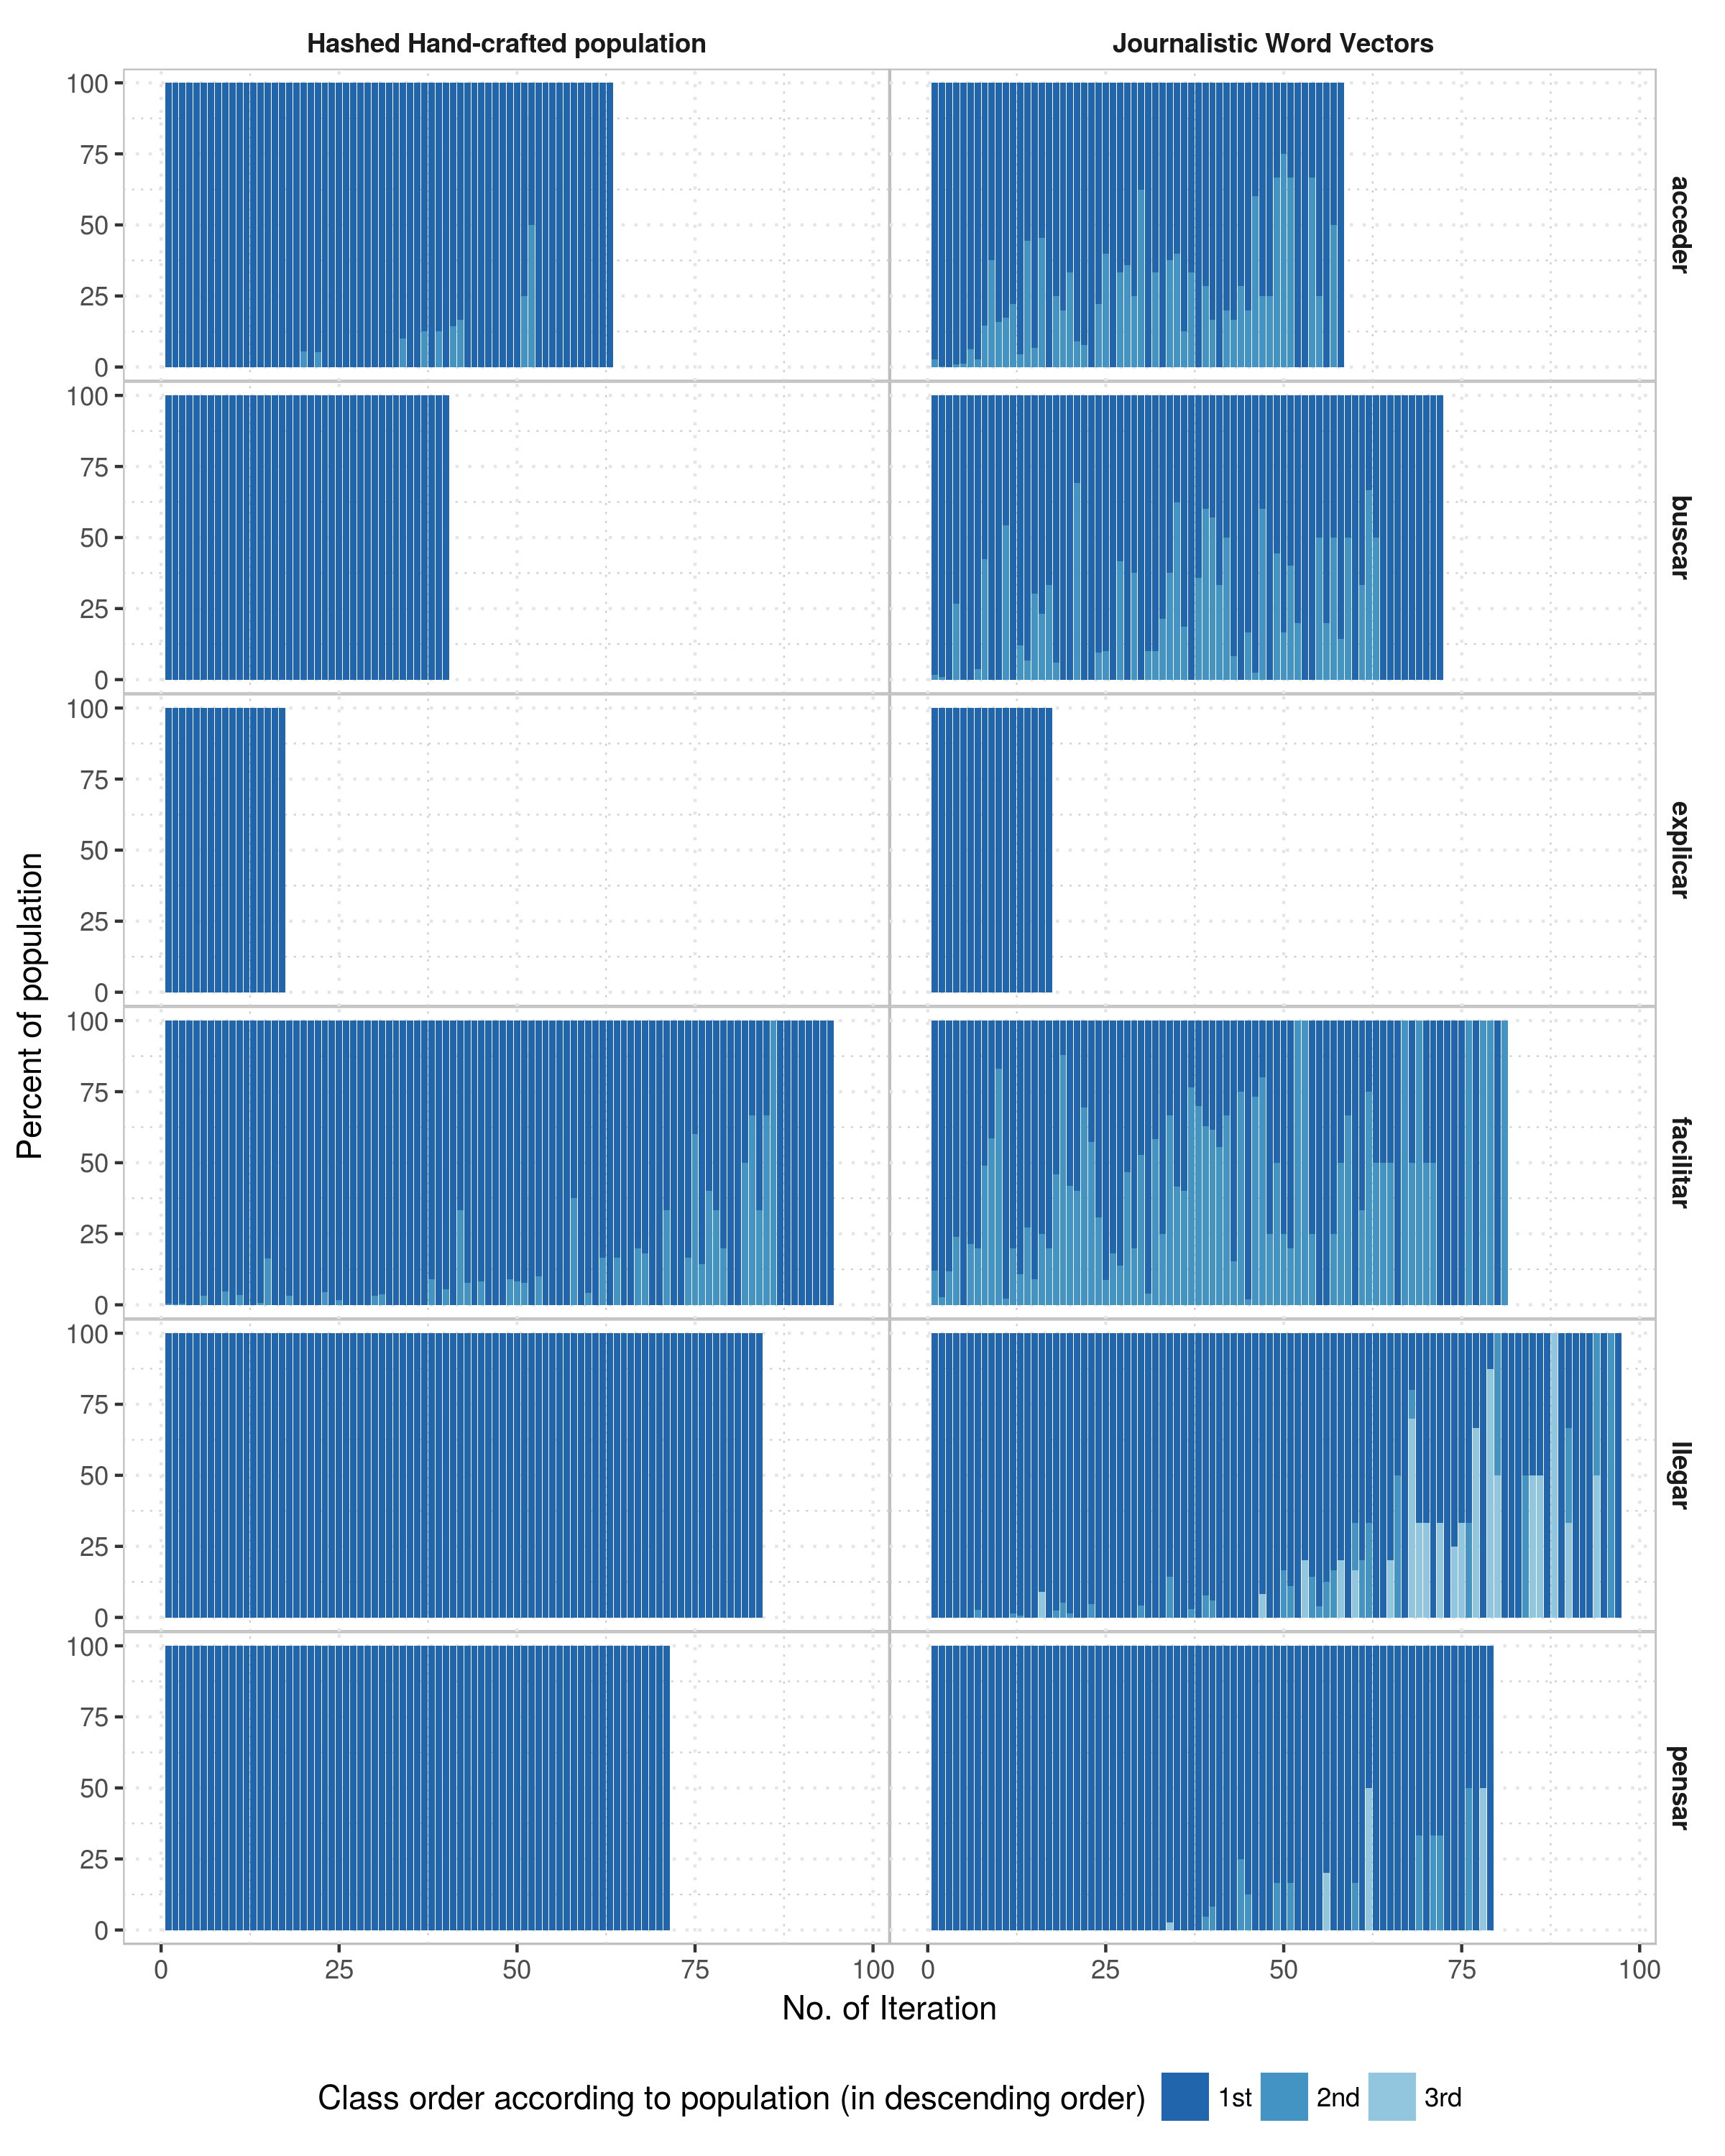
\includegraphics[height=.9\textheight,width=\textwidth,keepaspectratio]
    {plots/selflearning/population_add_per_class}
  \caption{Population added per sense on each iteration of self-learning as a
  proportional count of all the examples added in that iteration}
  \label{fig:self-learning:population_add_per_class}
\end{figure}

Figure \ref{fig:self-learning:population_add_per_class} shows the proportion of
examples added per class on each iteration. It is a stacked bar plot where each
bar represents the total examples added in the iteration, and each color in the
bar represents the proportion of classes automatically annotated as such. The
structure of the plot is the following:

\begin{itemize}
  \item Each row shows the results for a token lemma: ``acceder'', ``buscar'',
    ``explicar'', ``facilitar'', ``llegar'', and ``pensar''.
  \item Each column stands for a feature representation: hand-crafted hashed
    features and journalistic word vectors.
  \item The x-coordinate represents the iteration in the self-learning
    algorithm.
  \item The y-coordinate represents the percentage of examples automatically
    annotated and added to the model.
  \item Each bar plot represents the distribution of the examples added in the
    iteration. Each color of the stacked bar represents the class into which
    the examples were annotated.
\end{itemize}

This figure gives a better insight of what is happening on each iteration of
the algorithm and helps explain the distribution shown on Figure
\ref{fig:self-learning:population_distribution}, as it shows the proportion of
classes added in each iteration of each class.

I am able to see that the model trained with hand-crafted features practically
does not label the unlabeled data as something that is not the most frequent
class. This adds up to what is shown in previous paragraphs regarding
hand-crafted features having problems generalizing well to other domains.

The representation with word embeddings on the other hand is also affected, as
I saw in the previous figure, with the model diverging to the most frequent
class. However, there is a clear tendency for the model to also annotate
classes other than the most frequent one in the examples. And as I discussed in
Section \ref{sec:self-learning:hyp:1} the results of the self-learning
algorithm using word embeddings were quite superior to the ones obtained for
hand-crafted features. This means the word embeddings have a good impact on a
self-learning model as they help the classifier generalize better thus being
able to add new examples, even from different domains, to the model.

From this and the previous analysis I can conclude Hypothesis
\ref{hyp:self-learning:6} is false. Clearly it does not happen that the
self-learning model is adding new data uniformly distributed across classes.
Nevertheless word embeddings do help the model to add relevant data and not
labeling everything as part of the most frequent class. This is an interesting
line of future work as a deeper analysis, perhaps with manual evaluation, to
see how well word embeddings are helping to classify examples as part of the
less frequent classes.

\subsection{Hypothesis \ref{hyp:self-learning:7}}\label{sec:self-learning:hyp:7}

The last hypothesis I wanted to reject in this chapter is Hypothesis
\ref{hyp:self-learning:7}. The hypothesis states that the coverage given by the
features is uniform across classes. Recall that I showed in Section
\ref{sec:self-learning:hyp:4} that the number of features grew across
iterations of the self-learning algorithm, this was stated by Hypothesis
\ref{hyp:self-learning:4}. The previous section showed that the number of
classes is not maintained uniformly across the self-learning iterations, thus
it is natural to think this will happen with features as well. However, the
results I will show in this part are useful to throw some more light on the
results of the previous sections.

To test this hypothesis I want to measure two things: the raw count of the
features for each of the classes, and how strongly a feature is associated to a
class based on the pointwise mutual information it has with that class. These
results are obtained from Experiment \ref{exp:self-learning:4} which reports
the number of times a feature occurs with a class in the training dataset for
each iteration of the self-learning algorithm. To reduce the noise in the data
I filtered out all the pairs of $(features, classes)$ that co-occur less than 2
times.

\subsubsection{Features raw count}

The first view of the data I want to show is what comes to measure the results
of Experiment \ref{exp:self-learning:4} using the raw count. This shows the
number of unique features occurring with each class in each iteration of the
self-learning algorithm. In this view of the results, features can be present
in two classes at the same time, if they occurred more than twice with that
class, regardless of how strongly associated they are with the class.

\begin{figure}[htb!]
  \centering
  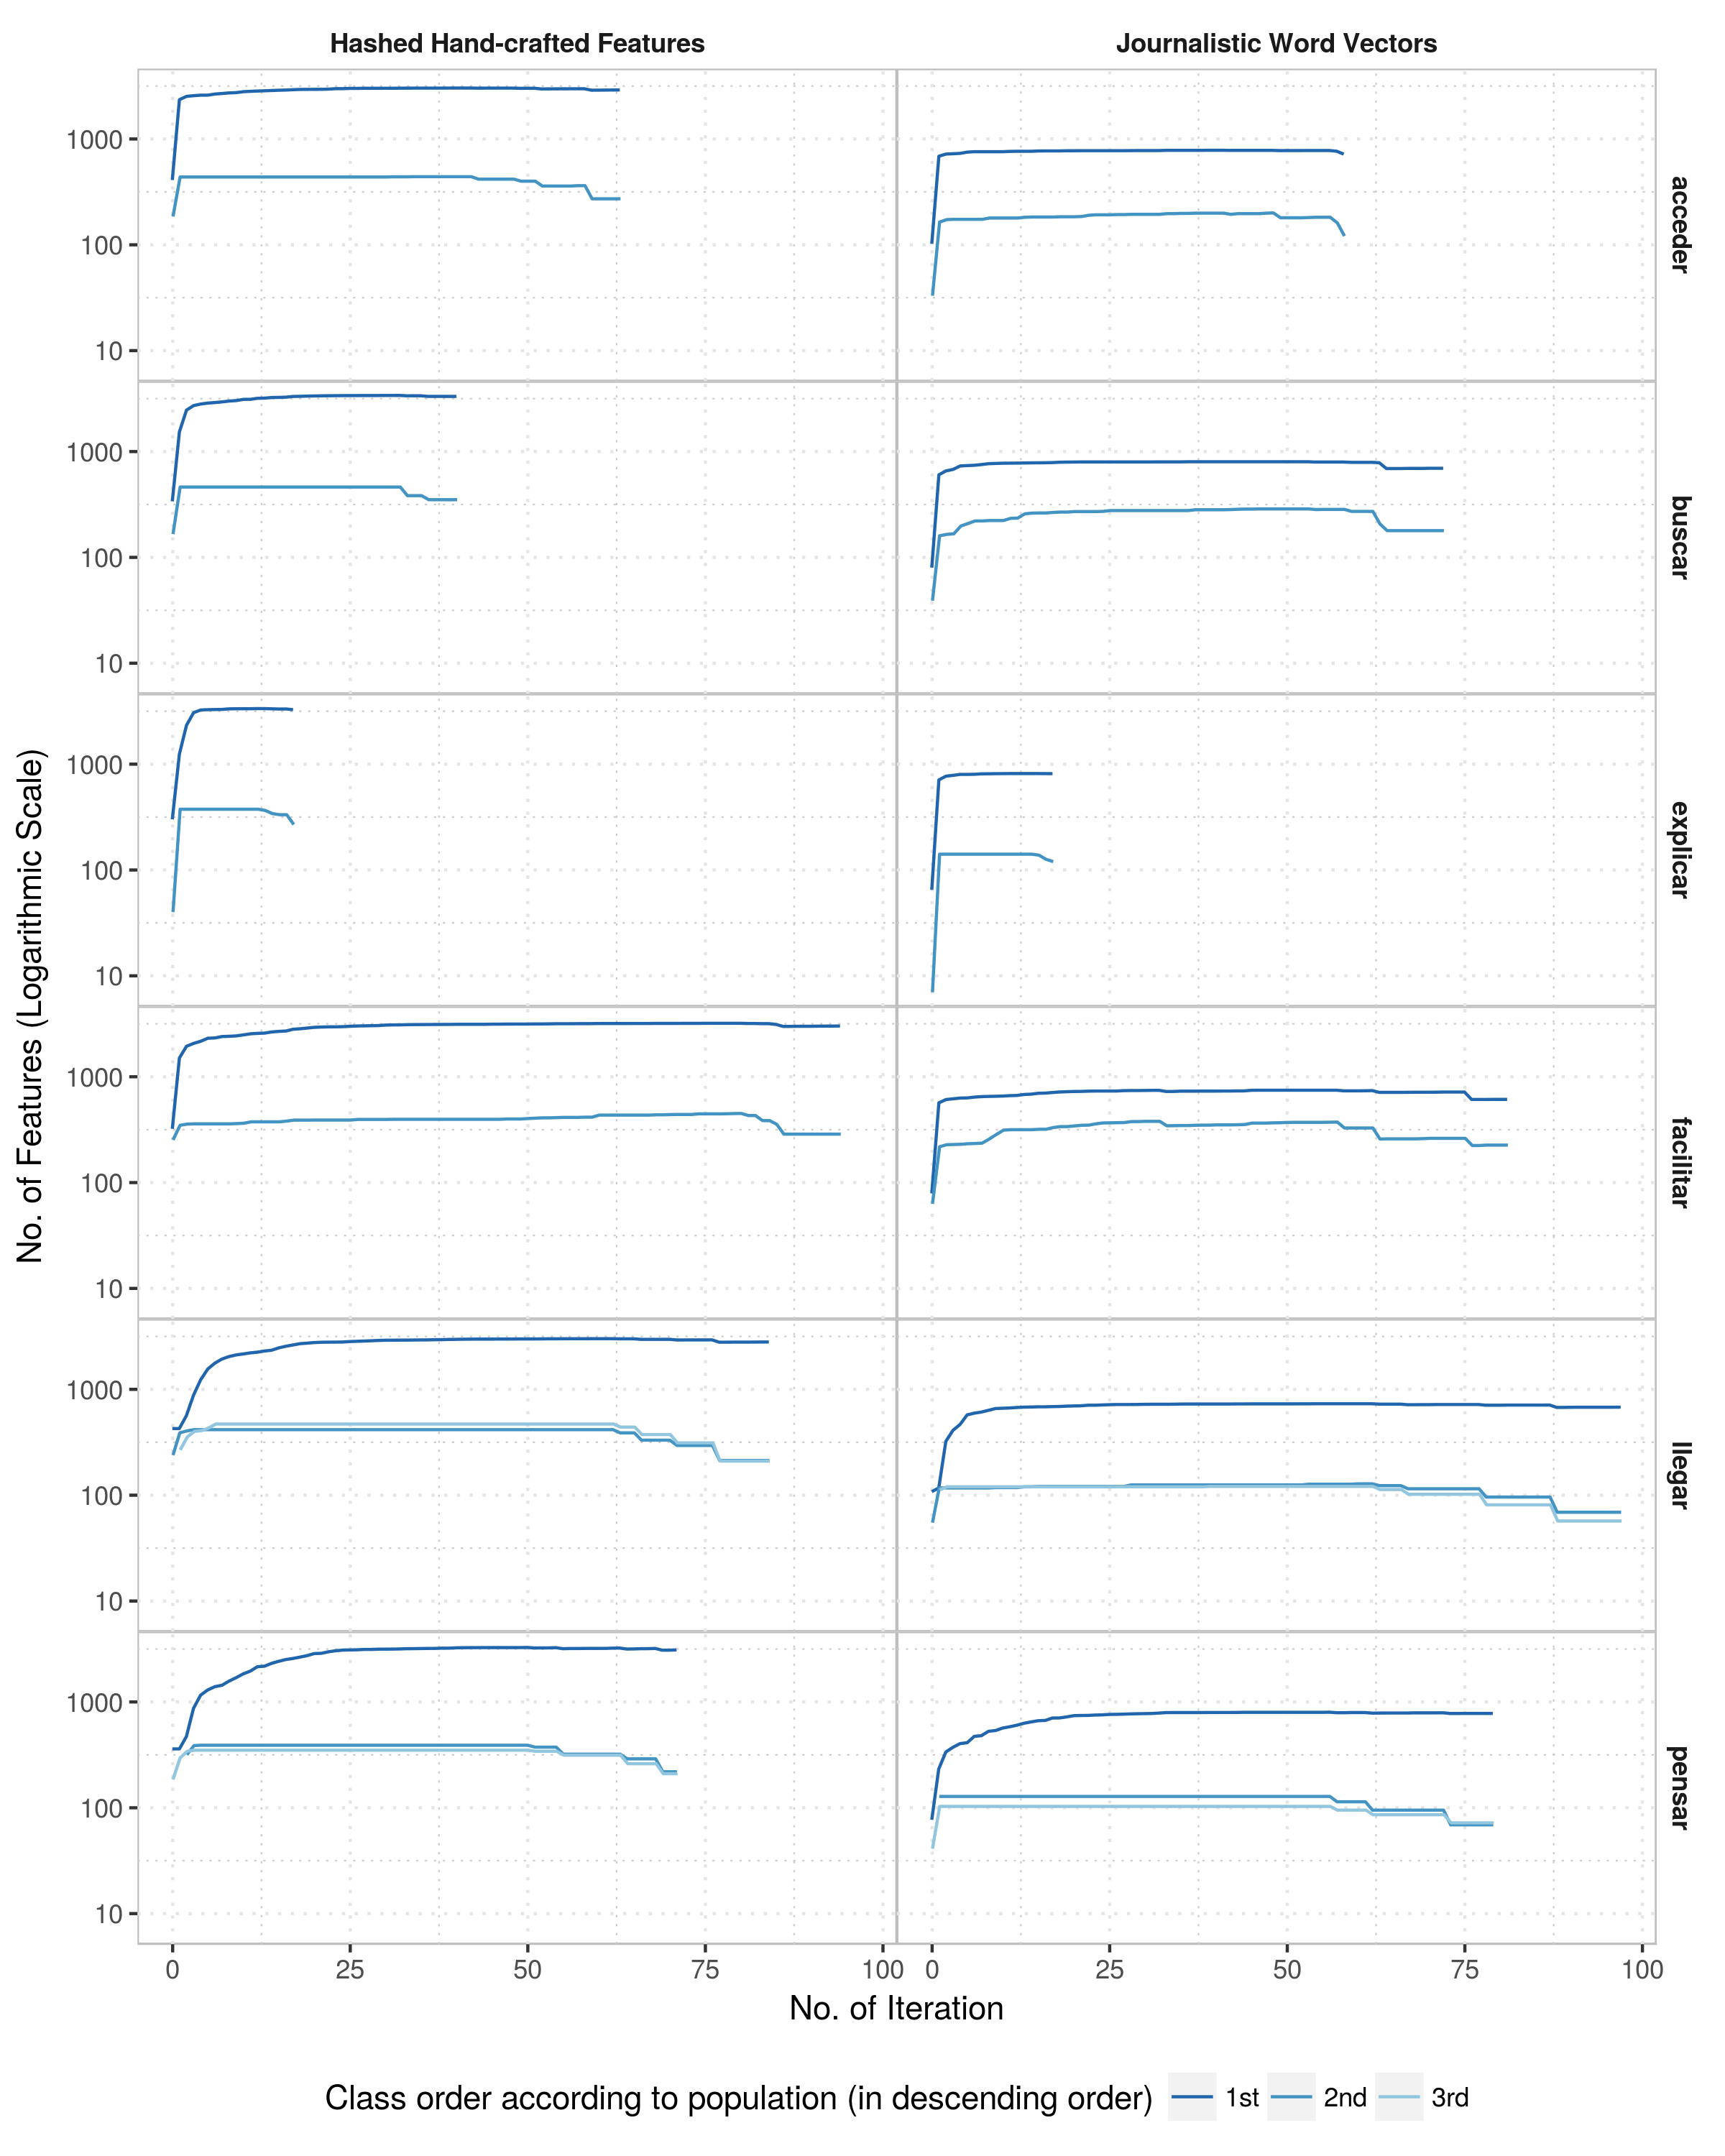
\includegraphics[height=.9\textheight,width=\textwidth,keepaspectratio]
    {plots/selflearning/features_growth_per_class}
  \caption{Features growth per class across self-learning iterations (in
  logarithmic scale)}
  \label{fig:self-learning:features_growth_per_class}
\end{figure}

Figure \ref{fig:self-learning:features_growth_per_class} displays the results
of counting the different features occurring with each of the classes in the
datasets. That is the total number of unique features up to that iteration
obtained both from the original supervised dataset and the automatically
annotated data. The figure shows a line plot with the following structure:

\begin{itemize}
  \item Each row shows the results for a token lemma: ``acceder'', ``buscar'',
    ``explicar'', ``facilitar'', ``llegar'', and ``pensar''.
  \item Each column stands for a feature representation: hand-crafted hashed
    features and journalistic word vectors.
  \item The x-coordinate axis represents the iteration number in the
    self-learning algorithm.
  \item The y-coordinate axis represents the raw count of unique features in a
    logarithmic scale. The scale selected is logarithm because, in comparison,
    the number of features of the most frequent class is an order of magnitude
    larger than those of the less frequent classes, and any variation (i.e.
    adding more features) of the less frequent classes is lost when compared to
    the most frequent class if I use a linear scale.
  \item Each line represents the number of features and the different colors
    represents the class that features belong to.
\end{itemize}

The figure shows that there is always a class for which the number of features
increases much more quickly and in a higher number than the others. This is a
consequence of the model diverging to the most frequent class. Most of the new
features also come from the first iterations of the algorithm and in the
following ones there are practically no more new features added. This is
particularly noticeable for the less frequent classes. As a consequence of
this, after some initial few iterations the algorithm diverges and all new
instances are directly added to the most frequent class. Thus in the last
iterations of the algorithm there are not new features for the less frequent
classes.

Once again the difference between hand-crafted features and word embeddings
resides in the pool of features. As I explained previously, the pool of
features that comprise the word embeddings model is much smaller than for
hand-crafted features. Nevertheless it is interesting that in some of the
lemmas the features grow for each class in the latter iterations for word
embeddings, while it does not for hand-crafted features. This comes from what I
saw in the previous Section regarding word embeddings helping the model
generalize better and annotate new classes besides the most frequent one.

There is an effective increase in the coverage, as many features are added to
the model. However these features belong mostly to a single class, the majority
class. In the following section I will show that this increase in the number
of features does not directly imply an improvement of the model.

\subsubsection{Features PMI}\label{sec:self-learning:featurespmi}

The second view of the data I want to show is based in the results of the
experiment measuring the correlatedness between features and classes. This is
given by the pointwise mutual information (PMI) between the features and the
associated classes given by Metric \ref{met:4}.

\begin{figure}[htb!]
  \centering
  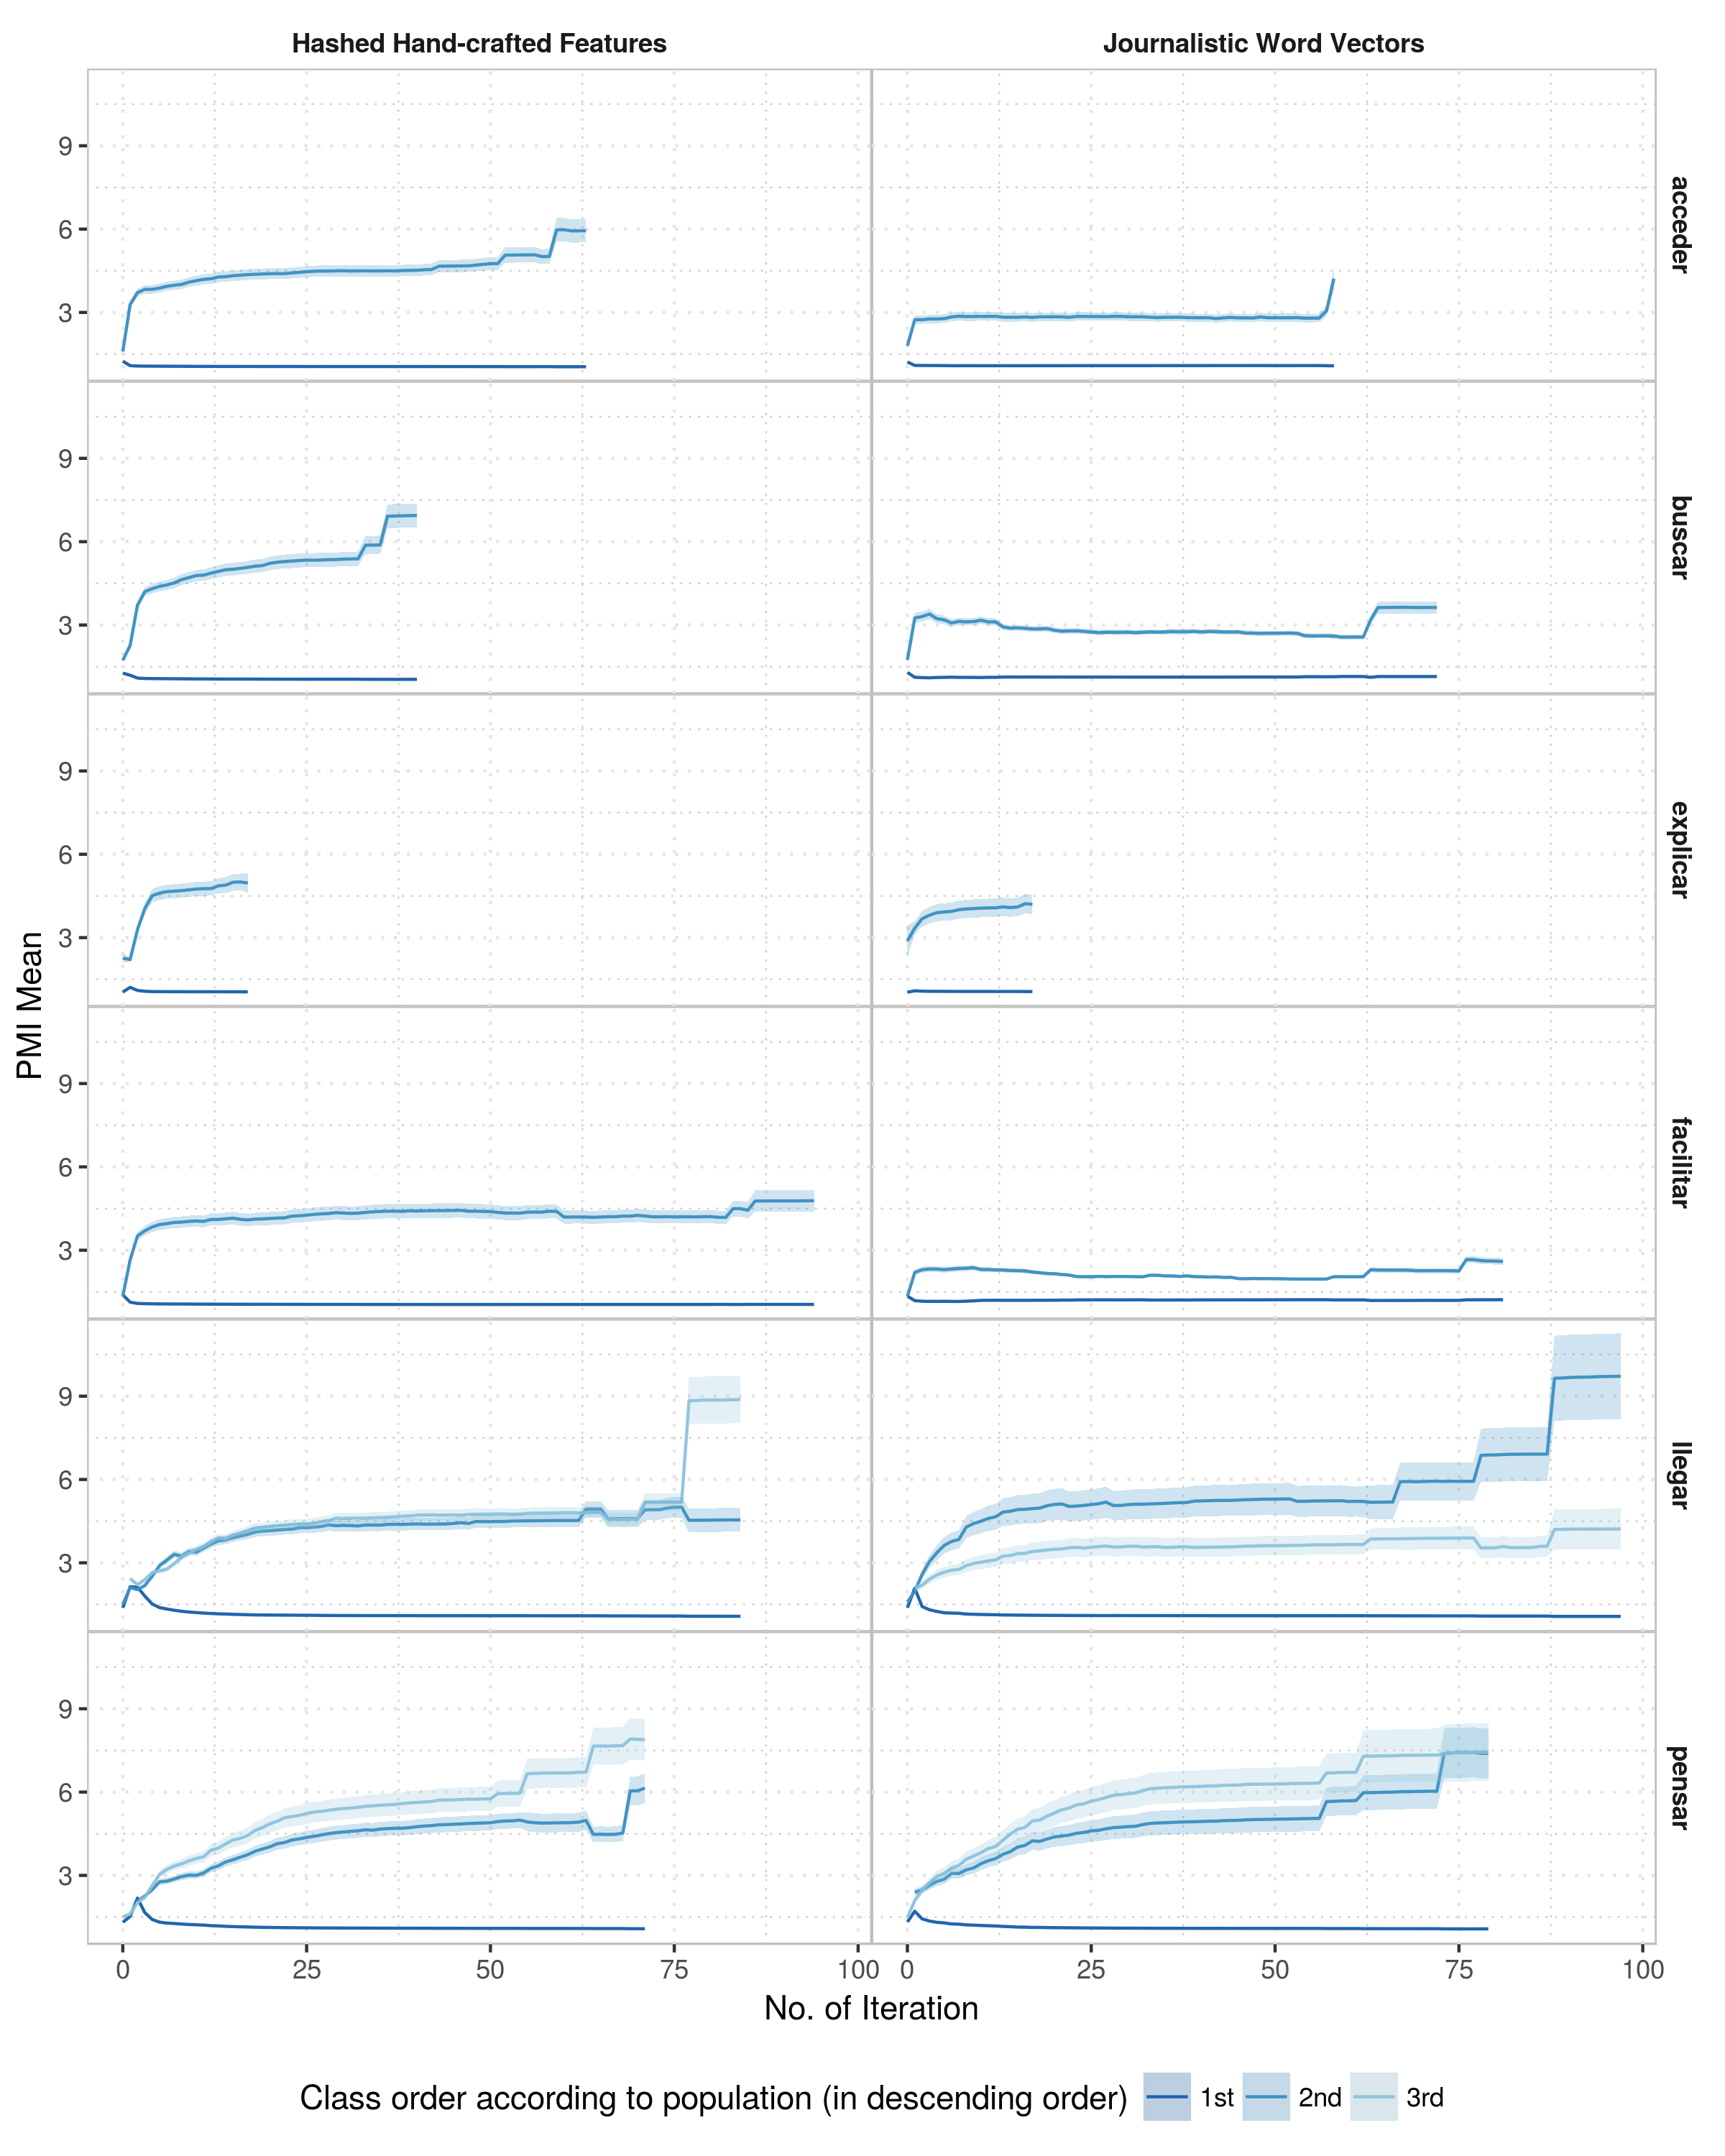
\includegraphics[height=.9\textheight,width=\textwidth,keepaspectratio]
    {plots/selflearning/features_pmi}
  \caption{Features pointwise mutual information with each of the classes
  across self-learning iterations}
  \label{fig:self-learning:pmi}
\end{figure}

Figure \ref{fig:self-learning:pmi} displays the mean and standard error of the
mean of the pointwise mutual information between features and classes across
the self-learning iterations. Thus it is higher when the features associated to
a class are associated more strongly to the class. Recall that the metric
associates each feature to the class it has a higher PMI with. The figure shows
a line plot with the following structure:

\begin{itemize}
  \item Each row shows the results for a token lemma: ``acceder'', ``buscar'',
    ``explicar'', ``facilitar'', ``llegar'', and ``pensar''.
  \item Each column stands for a feature representation: hand-crafted hashed
    features and journalistic word vectors.
  \item The x-coordinate axis represents the iteration number in the
    self-learning algorithm.
  \item The y-coordinate axis represents the raw count of unique features in a
    logarithmic scale.
  \item Each color represents a class.
  \item The line of darker color in the middle represents the mean of the PMI
    for the class and the shadowed area represents the standard error of the
    mean for that PMI.
\end{itemize}

Different from the previous figure, now the classes with a smaller number of
features are the ones having the larger values in the plot. It seems that in
classes with a smaller number of features, these are associated more strongly
to the class. In contrast, in classes with a bigger number of features, these
are associated more weakly. It seems that the most frequent class is working as
a ``catch all'' for new examples, mostly those without features strongly
associated to any other class, and because of the algorithm's tendency to
annotate examples to it. Then, the features in these new examples are
associated to that class. However, these features are not strongly related to
that class, because they belong to examples that have been classified into the
class by weak reasons, like the probability of the class or the lack of
characterizing features. This makes these features not a good parameter to help
discriminate this class. On the other hand the features for the less frequent
classes become much more discriminative of such classes because new examples
are only classified into those classes when there is strong evidence that they
belong to the class, that is, when evidence is stronger than the default to
classify them into the majority class.

Even if it looks like the classifier's coverage is increasing, because of the
number of features doing so, from this data there is a clear indication that it
is not like that because the new features belong mostly to the most frequent
class and do no contribute to increase the certainty of the model, which is
reflected on a low mean of the PMI with the most frequent class.

On the other hand, those features that are associated to the less frequent
classes do so with a strong association to the point that as the self-learning
iterations add new examples the features become more discriminative of this
less frequent classes. However, the number of these features does not increase
as much, as was shown in the previous section.

\subsection{Summary}

The results of the evolution of certainty and tendency to overfit in the model
give the impression that hand-crafted features have less variance than word
embeddings. However, a more detailed analysis shows that even though the
variability is less in hand-crafted features, the reason behind this is that it
only adds new examples of a particular class, the most frequent one. This is
not the case for word embeddings.

Word embeddings show more variability in the tendency to overfit and the mean
of the certainty as it is effectively adding new examples annotated into
classes that are not only the most frequent one. Moreover, Figure
\ref{fig:self-learning:population_add_per_class} shows there are some instances
where only elements of the less frequent classes are added.

\section{Conclusions}\label{sec:self-learning:conclusions}

In this chapter I have presented an approximation to self-learning to overcome
the problems of overfitting and coverage presented in the previous chapters.
My initial hypothesis was that the overfit is caused by the low number of
examples and that increasing such number helps reducing it.

I saw that adding new examples effectively helps reducing the overfit in the
initial iterations. However, self-learning is biased to the most frequent
class. This makes the model add many examples to that class, ignoring the less
frequent classes. This is particularly noticeable for hand-crafted features.

To draw this conclusion I defined some subhypotheses in the beginning of the
chapter. The experiments done to test these hypotheses gave me the possibility
to draw the following conclusions.

Hypothesis \ref{hyp:self-learning:1} that the performance of the model over a
held-out test dataset improves after the self-learning algorithm was shown
false for the case of hand-crafted features but I could not obtain conclusive
results to reject it with respect to word embeddings. In the latter case the
results depended on the lemma, as for some the performance decreased but for
others it increases or remains the same. An important results I could gather
from this is that hand-crafted features had a steeper drop in performance than
word embeddings, a sign that the representation fits the labeled dataset well
but fails to generalize.

Hypothesis \ref{hyp:self-learning:2}, which stated that the model's average
certainty on unseen examples in each iteration is increased, is rejected in
light of the obtained results. This is because there is a clear tendency of
the certainty of the mean that the algorithm has over unseen data to decrease
across iterations. 

Hypothesis \ref{hyp:self-learning:3}, which states that overfitting is reduced
across self-learning iterations, is mildly rejected. The fact is that the
number of examples effectively reduced overfitting in the first iterations of
the algorithm. However, as I do not use this as a stopping criterion in the
algorithm, when it starts to diverge to the most frequent class, the tendency
to overfit increases.

Hypothesis \ref{hyp:self-learning:4} stated that the coverage of the model
increases as a result of increasing the number of features associated to this
model. The number of features associated to the model indeed increases as the
results did show. These results are enough to accept the stated hypothesis.
However, as I saw in the results associated to Hypothesis
\ref{hyp:self-learning:7}, which conclusions are in the next paragraphs, these
results are not enough to show that there is an indication of the model
effectively increasing coverage as a result of increasing the number of
examples.

The previous hypotheses were formulated with the idea to accept them. This was
not exactly the case. However, the other three hypotheses in this chapter were
formulated with the idea they would be rejected.

Hypothesis \ref{hyp:self-learning:5} states that the performance of the
self-learning algorithm over all the classes is improved. The hypothesis is
rejected because only the performance of the most frequent class increases
through iterations of the self-learning algorithm, while the rest of the
classes show a degraded performance.

Hypothesis \ref{hyp:self-learning:6} states that the representativity of each
class in the dataset is kept through all the iterations of the algorithm. The
hypothesis is also rejected. The results show that new examples added to the
model belong mostly to the most frequent class and the distribution of the
classes is highly biased across the iterations. In particular, hand-crafted
features have the worst performance in this as the model only adds examples of
the most frequent class. Word embeddings have better performance as the
algorithm adds examples of the less frequent classes as well. This last has
relation to what happens in the results of the previous hypothesis where there
are some cases where the less frequent classes' performance does not drop to
zero as in hand-crafted features.

Hypothesis \ref{hyp:self-learning:7} states that the coverage of the features
is uniformly distributed across the classes. The results obtained serve to
prove the hypothesis false. This hypothesis is related to Hypothesis
\ref{hyp:self-learning:4} which states that the number of features associated
to the model increases after the self-learning iterations, which is true, but
not in the way the model needs in order to effectively increment the coverage.
This is because the certainty of the model does not increase with the number of
features. In a detailed analysis it is seen that most of the features are
weakly associated to the classes (in particular to the most frequent class).
So, their contribution to the model is small. Thus a bigger number of features
does not imply a better model, not even better coverage, because they are not
discriminative enough. A possible cause of this is that, when the model starts
to overfit, the most frequent class begins to coopt elements that are not part
of the class. This makes the model drift and starts to have less certainty over
new examples.

As I saw in the results of this chapter, the biggest problem for self-learning
is the tendency to diverge and add everything to the most frequent class. A
way of attacking this problem is using techniques which help stop that bias.
There are different ways to do so. One is by re-sampling the data. I only
explored random oversampling of the less frequent classes, which did not prove
useful. Other re-sampling methods include the random sub-sampling of the most
frequent class or a mix of both.

In the next chapter I will explore a technique based on human annotation which
selects examples based on high uncertainty and give that to a domain expert in
order to correctly annotate them. The idea is that this examples will help the
model better define the decision boundaries over the most frequent class, which
is something the self-learning algorithm is not doing well.

Future work of this chapter includes the change of the stopping criterion for
something to stop once the model becomes to overfit again (the spread between
training error and validation error grows). Another line of future work is a
more general analysis of all the lemmas, and some more specific analysis on
some more lemmas beside the selected tokens.

I also have to do more thorough analysis of the certainty the model has over
new examples (i.e. previously unseen) and why it becomes so irregular as the
algorithm's iterations go further.

Finally, as word embeddings proved to have interesting results and, unlike
hand-crafted features, they did not drift so quickly or so firmly to the most
frequent class, it would be interesting to do some manual evaluation and error
analysis to see what is happening under the hood.


\chapter{Active Learning}\label{chapter:active}
\section{Overview}

In Chapter \ref{chapter:supervised} I concluded that the number of examples has
a direct impact in the performance of a supervised \vsd~algorithm. I also
explained that small supervised corpora have a direct impact in both the
coverage and the tendency to overfit of a supervised model. To attack the
latter I saw in Chapter \ref{chapter:embeddings} that the use of word
embeddings, although decreasing performance in the test portion of the
supervised corpus, did help in the tendency to overfit of a model. In the
self-learning approach, word embeddings show an interesting performance as
well: even if coarse accuracy figures are more or less comparable for
hand-crafted features and for word embeddings, the latter have better recall in
minority classes and incorporate more informative features.

In Chapter \ref{chapter:self-learning} I explored self-learning as a joint
semi-supervised method. The original idea of using this method was to overcome
the problem regarding the model's coverage by adding new data, that is
automatically annotated, to the training set. The chapter also gave me more
insight of the benefits of using word embeddings as a representation when faced
with a task where the domain changes. However, there is a challenge in the
method of self-learning: the tendency of the method to add only examples of the
most frequent class.

This chapter introduces another semi-supervised joint learning framework: {\em
active learning}. Like self-learning, active learning consists in expanding the
training examples with new data provided by an unannotated corpus. Also, as a
wrapper method, it does so by training a model from labeled data and improving
that model with new labeled data obtained from the unlabeled corpus. 

The difference between self-learning and active learning lies in how the last
method labels the unlabeled data. This is not done automatically, but by the
means of an oracle, i.e. an annotator who has high certainty over the data it
is labeling (generally speaking, this is done by a human annotator, more
specifically a domain expert).

But this is not the only difference, since the way unlabeled instances are
selected for annotation also differs from the method used by self-learning.
While self-learning relies on the certainty the algorithm has over the data to
safely assume the given label is right, active learning seeks for data which,
once labeled, will yield the biggest improvement on the model. This data is
near the decision boundaries of the model and is generally more difficult to
tell it apart from data with other labels. 

One of the most popular techniques to select data that will improve the model
is {\em uncertainty sampling}. I briefly introduced it in
Chapter~\ref{chapter:general_background}. In this technique the underlying
hypothesis is that those instances on which the classifier has the least
confidence are the ones closest to the decision boundary and thus the ones to
make the most difference after being labeled.

In our setting, those instances which have the most impact on a model are
typically the ones that are underrepresented in the labeled dataset. And this
is precisely where active learning overcomes one of the problems of
self-learning: the bias to the most frequent class. As self-learning is a model
based on certainty, this implies that it will add mostly instances of the most
frequent class (typically the one the model has better certainty about, even if
only by probability). Active learning, on the other hand, helps the model spot
useful instances of those underrepresented classes in the labeled dataset and
provides the means to add them for a broader coverage.

Moreover, active learning not only adds examples of the pre-existing classes of
the model but of new classes as well. Remember in previous chapters I explained
that some classes of the SenSem corpus were filtered out because they did not
had enough occurrences in the supervised dataset. Besides those cases there are
also senses in the SenSem lexicon that did not have any examples in the
annotated corpus. As the labeled corpus is domain specific, this results in
the corpus not having examples of some of the possible senses. However, when
applying active learning over an unlabeled corpus of a general domain, examples
of these senses pop up in the flow of the algorithm. This is a common
phenomenon as the certainty the model has over those examples it never saw
before will be low, thus it will be picked up by the uncertainty sampling
technique. There are even senses that are directly not taken into account by
the resource, but these are left out as it is outside the scope of this thesis
because it requires the extension of the SenSem lexicon.

Regarding what is stated in the previous paragraph there is a remark to do
about self-learning. Recall that the last chapter showed that with the
self-learning model the certainty over new examples decreased in each
iteration. Thus it is possible that the self-learning algorithm was marking
those examples the model had less certainty about as part of the most frequent
class. However these examples were not even part of the initial labeled dataset
as the classes of those examples are not present.

This chapter will test the following hypothesis:

\begin{hypothesis}\label{hyp:active}
  Active learning improves the performance of a supervised model by reducing
  the bias of the initial dataset that is correlated to overfitting of the
  supervised model.
\end{hypothesis}

In order to accept or reject such hypothesis, I divide it in more specific
ones:

\begin{subhypothesis}\label{hyp:active:1}
  The representativity of the population for each class in the dataset is
  maintained through all the iterations of the algorithm.
\end{subhypothesis}

\begin{subhypothesis}\label{hyp:active:2}
  The active learning algorithm increases the number of features associated to
  the model more quickly than self-learning, which is an indicator of a quicker
  increment in the coverage of the model.
\end{subhypothesis}

These hypotheses will be tested using the following layout:

\begin{itemize}
  \item Experiment \ref{exp:active:2} records the number of occurrences per
    each class in the training dataset on every iteration of the active
    learning algorithm. The population of the classes is measured by the
    proportional count with respect to the whole training dataset. The results
    of this experiment, shown in Section \ref{sec:active:hyp:1}, serve to
    accept Hypothesis \ref{hyp:active:1} which states that the population of
    all the classes is maintained along the algorithm's iterations.
  \item Experiment \ref{exp:active:3} records the number of times a feature and
    a class occur together in an instance of the training dataset. I measure
    these results using two different metrics. First, in comparison to the
    results gathered from Experiment \ref{exp:self-learning:4} (which records
    the same data but for the self-learning algorithm), I use the normalized
    count of features by number of examples per iteration (Metric \ref{met:6}).
    It is necessary to normalize because the number of examples added in each
    active learning is much smaller than in self-learning, thus normalization
    is necessary for a meaningful comparison. On the other hand I analyze the
    PMI along the iterations for the classes and the features associated to it
    (Metric \ref{met:4}). The results are shown on Section
    \ref{sec:active:hyp:2} and serve to accept Hypothesis \ref{hyp:active:2}
    which states that the active learning algorithm improves the model's
    coverage quicker than self-learning.
\end{itemize}

In Section \ref{sec:active:previous} I revise some previous work in active
learning in general and also specifically applied to \vsd.

In Section \ref{sec:active:methodology} I go through the relevant items that
concern the experimentation in the chapter. Most of the methodology is very
similar to that in previous chapters, I mostly provide pointers to the sections
where this methodology is first described. In particular Section
\ref{sec:active:algorithm} explains the fine detail of the active learning
algorithm, e.g. the stopping criterion the algorithm uses, how the instances to
annotate are selected and how the annotation is carried out, as well as some of
the difficulties of the annotation. 

Section \ref{sec:active:results} reports the results of the experiments and
analyzes them in order to accept the stated hypotheses of the chapter.

Finally Section \ref{sec:active:conclusions} draws the conclusions of this
chapter, recapitulating the Hypotheses and the implications of accepting or
rejecting them according to the evidence gathered in the results. It states the
shortcomings of the methods explored in this chapter and what I want to
accomplish on the next. It ends by outlining future work.

\section{Relevant work}\label{sec:active:previous}

Active learning is a task for semi-supervised learning, based on the key idea
that if the learning algorithm is allowed to choose the data from which it
learns it will perform better with less training. A very complete survey in the
area is the one done by Settles \cite{settles.tr09}. It covers all the main
topics in the area of active learning.

A particularly important subject in active learning is the strategy to select
the instances to present to the oracle. Different strategies have been studied,
being {\em uncertainty sampling} the most intuitive and popular one
\cite{Lewis94heterogeneousuncertainty} and the one used in this chapter. For
other strategies refer to Section \ref{sec:general_background:active} of
Chapter \ref{chapter:general_background}.

One of the main problems in applying active learning to natural language
processing tasks is class imbalance, something common in the are. In this
cases, uncertainty sampling not always proves being the best way to select data
given some difficulties it arises as I will explain in Section
\ref{sec:active:difficulties}. There are some approaches to deal with it, but
nothing definitive.

In particular, Dligach and Palmer \cite{dligach2011good} applied active
learning to verb sense disambiguation. They explored the benefits of using an
unsupervised language model to select seed examples as a starting corpus for an
iterative active learning approach.

\section{Methodology}\label{sec:active:methodology}

This chapter explores the use of active learning with a human annotator to
expand a model trained with labeled data. Like the self-learning algorithm in
the previous chapter, active learning is also a {\em wrapper}. The algorithm
uses a supervised classifier to select instances from the unlabeled data and
gives it to a human to verify it.

The objective of this chapter is to show the tendencies I have found using
active learning. I do not present an exhaustive analysis of active learning, as
it requires annotating resources using human experts which I are outside the
possibilities of research of this thesis. The idea is to analyze preliminary
results which can help as an initial start for future work using more
resources.

\subsection{Resources}\label{sec:active:resources}

In this chapter I keep using the datasets I have been working on so far: the
SenSem corpus as labeled corpus and SBWCE as the unlabeled.

Analyzing active learning was the main reason to reduce the analysis to some of
the lemmas in the lexicon. The selected lemmas on which I make my analysis are:
``explicar'', ``pensar'', ````acceder'''', ``llegar'', ``buscar'' and
``facilitar''. A detailed explanation of this is done in Section
\ref{sec:self-learning:resources}, please refer to it for more information.

The SenSem corpus is used as the annotated seed on which the active learning
algorithm starts. For a detailed description of the resource please refer to
Section \ref{sec:supervised:sensem}.

The unlabeled data source for new instances to give to the human expert to
manually annotate is taken from the SBWCE corpus. Please refer to Section
\ref{sec:embeddings:sbwce} for more details on the corpus. The corpus is the
one pre-processed with Freeling obtained by the methodology described in
Section \ref{sec:self-learning:sbwce}. Please refer to that section for more
details on how this is done.

\subsection{Features}

The features used in this part are the same ones used in the previous chapters.
Both hand-crafted features using the hashing trick and word embeddings follow
what has been discussed in all the previous chapters.

For more information on the detail of what are the hand-crafted features used
in this chapter please refer to Section \ref{sec:supervised:features}. For
detailed information on how to deal with the expansion of features given by the
new examples added to the model please refer to Section
\ref{sec:self-learning:handcrafted}.

The word embeddings are the ones trained from the journalistic corpus described
in detail in Section \ref{sec:embeddings:journal}. The method for combining
them into an instance is the concatenation of word vectors described in Section
\ref{sec:embeddings:embeddings}.

\subsection{Classifiers}

As in self-learning, active learning is a wrapper method that is built around a
supervised classifier. The selected classifier is the same as in the previous
chapters. I use a multilayer perceptron with three layers of size 500, 250 and
100 each.

\subsection{Active learning algorithm}\label{sec:active:algorithm}

The active learning algorithm follows the same structure as the self-learning
algorithm described in Section \ref{sec:self-learning:algorithm}, taking as
input almost the same initial parameters:

\begin{itemize}
  \item A labeled training dataset to train the initial supervised model.
  \item A labeled test dataset to report the model performance before and after
    finishing all the iterations of the self-learning algorithm.
  \item An unlabeled dataset to get the new data to annotate automatically.
  \item A probabilistic classification algorithm, to use in the process of
    automatic annotation.
  \item A maximum number of elements to annotate each iteration.
  \item A tolerance error for the stopping criterion.
\end{itemize}

The fundamental differences in this case reside in the following items: (i) how
the model selects instances to label from the unlabeled dataset, (ii) how those
instances are annotated, (iii) how the model decides whether new instances are
to be included in the training corpus, (iv) how the algorithm finishes.

\subsubsection{Instance selection and annotation}

In each iteration of the algorithm, once the classifier is trained with the
examples gathered so far (both part of the initial seed dataset or from the
oracle's annotations) the algorithm applies the classifier to the whole pool of
unannotated data. From the automatic annotation of that pool of unlabeled
examples, the algorithm takes the ones the classifier is less certain about and
presents them to the oracle for manual annotation. This is called {\em
uncertainty sampling}, i.e. selecting those instances for which the certainty
of the classifier is low. It is assumed that those instances are near the
decision boundaries of the model. The intuition behind using this method
instead of randomly giving the oracle examples to annotate is that these
examples will have the largest impact on the final model, that is, the model
will improve its accuracy the most. This is because the classifier gains
confidence on those classes and instances it has less information about in the
seed labeled corpus. This is a way to optimize learning with a given amount of
training data, by improving the quality (not the quantity) of the training
examples.

Unlike self-learning, which selects all the instances over a threshold, in
active learning there is a maximum number of possible instances. It is given as
an initial parameter of the algorithm. This number is selected empirically and
should be large enough to make a difference in the new model but not too big to
have the oracle devoting too much time annotating, since active learning gives
an intelligent way to minimize the annotation effort. After some
experimentation, the number of 10 examples per iteration was selected as the
base for the experiments in this chapter.

The oracle annotates the examples selected by the active learning algorithm,
which are then added to the model. There is however a problem, as I explained
before: the initial annotated corpus may not have a correct label for some
examples because it was not considered originally when designing the lexicon.
In those cases, to reduce the number of possibilities to consider and as it is
outside the scope of this thesis to extend the resource, I decided to ignore
examples belonging to an sense not present in SenSem.

\subsubsection{Validation of the model and early stopping}

Once the instances are annotated by the oracle, the next step is, like in
self-learning, to add them as new training examples. However, the algorithm
first checks the impact of adding these new examples to the model, by assessing
the performance of the model with the bigger training corpus.

For self-learning, this was done using a validation dataset extracted from the
original dataset. I originally thought about using cross validation over the
training dataset in self-learning, but finally I abandoned the idea. The
tendency of the self-learning algorithm to add everything as part of the most
frequent class may have introduced bias in that method of validation.

For active learning however this is not a problem. As the annotation is not
left to the classifier but to a human, the tendency to annotate everything as
the most frequent class does not prevail as much. I decided then to use
cross-validation over the training examples and see the mean of the
misclassification error obtained from it as the metric to validate the impact
of the new training examples in the model. 

The main reason to use cross validation over the training dataset and not a
validation dataset like in self-learning is because unlike in self-learning,
this algorithm may add examples of classes not seen by the model so far.
Remember some senses were filtered out from the SenSem corpus because they did
not have enough available instances. Moreover, some of the senses in the
lexicon do not have any examples at all. Well, these senses occur in a larger
corpus like SBWCE, and as the classifier will not have enough information
initially over those senses, it is likely that examples of those are chosen to
give to the oracle using the uncertainty sampling technique.

As new examples of unseen classes may be added to the training data this might
result on the validation corpus not reflecting the model's real performance.
The reason behind this is that the validation corpus does not have any
information regarding the new unseen classes the model is adding.

Once the algorithm calculates the misclassification error from the
cross-validation over the training dataset it applies the same principle the
self-learning algorithm did, it compares it to the minimum error obtained so
far and gives a tolerance of maximum 10\% less than random chance. If the error
in the new model is larger than that, the algorithm discards the model and
returns the last model obtained so far. As it requires human annotation, the
algorithm also provides the option for the human to stop iterations whenever he
wants.

\subsubsection{Difficulties in the annotation}\label{sec:active:difficulties}

There were two major difficulties when dealing with the annotation of the
examples selected by the algorithm based on high uncertainty: ambiguity and
coverage of the classes available in the resource.

Since the inventory of senses is human given, it is arbitrary, shaped by the
humans creating the resource and the final objective such resource has. This
means that depending on these variables, the inventory of senses may be coarse
or fine-grained. This of course affects the possibilities to annotate, as a
more coarse inventory may fall in the problem of having senses that are
suitable for more than one sense. As the algorithm selected those instances
that are near decision boundaries, a common problem is giving the oracle
examples that are ambiguous even for the oracle to discern.

Besides the problem of having senses with blurry decision boundaries, which
overlap with each other, the other problem the resource may have is lack of
coverage. Thus there are some examples that are not suitable for any of the
senses given in the resource. This is particularly common since an important
part of the SBWCE corpus consists on books written in old Spanish (i.e. the
ones compiled in the Wikisource initiative). Thus there are some senses which
fell into disuse and were not considered in the construction of the resource.

\subsection{Experiments}\label{sec:active:experiments}

There are three major experiments I did in this chapter: one to compare the
performance of the active learning algorithm with the self-learning algorithm,
and two others to test the hypotheses.

First, Experiment \ref{exp:active:1} is very similar to Experiment
\ref{exp:self-learning:1} in Chapter \ref{chapter:self-learning}. The
experiment is not aimed at testing any of the hypotheses of this chapter but
rather as a comparison with the previous chapter. It basically tests the active
learning algorithm and how it affects the performance of the supervised
classifier over the held-out test data.

\begin{experiment}\label{exp:active:1}
  \begin{enumexp}
    \item Train a model with the supervised training dataset.
    \item Evaluate the model over the test dataset.
    \item Run the active algorithm until it stops.
    \item Evaluate the model obtained with the active algorithm over the test
      dataset.
  \end{enumexp}
\end{experiment}

Experiment \ref{exp:active:2} is the first experiment to test a hypothesis in
this chapter. The experiment is to evaluate the representativity of the
population for each class across the active learning iterations. It is done to
test Hypothesis \ref{hyp:active:1}, which states that this representativity is
maintained through all the iterations of the algorithm. This experiment is
based on Experiment \ref{exp:self-learning:5} in the previous chapter.

\begin{experiment}\label{exp:active:2}
  \begin{enumexp}
    \item Record the number of times each class occurs in the supervised
      training dataset.
    \item Run an iteration of the active learning algorithm.
    \item Record the number of times each class occurs in the new training
      dataset comprised of the supervised data and the new annotated
      examples.
    \item Repeat the previous step for each iteration of the algorithm.
  \end{enumexp}
\end{experiment}

Finally, to test Hypothesis \ref{hyp:active:2} regarding the number and
association of features to classes, there is Experiment \ref{exp:active:3},
which is based on Experiment \ref{exp:self-learning:4} in the previous chapter.
The experiment records the number of times each tuple of classes and features
appear in the dataset.

\begin{experiment}\label{exp:active:3}
  \begin{enumexp}
    \item Record the number of times a tuple $(class, feature)$ occurs for each
      class and each feature of the supervised training dataset.
    \item Run an iteration of the active learning algorithm.
    \item Record the number of times a tuple $(class, feature)$ occurs for each
      class and each features of the training dataset comprised of the
      supervised data and the automatically annotated instances.
    \item Repeat the previous step for each iteration of the algorithm.
  \end{enumexp}
\end{experiment}

\subsection{Metrics}\label{sec:active:metrics}

To report the results of Experiment \ref{exp:active:1} I use the F1-score for
each class in the test dataset of the token lemmas, for each of the three
algorithms: supervised, self-learning and active learning.

For Hypothesis \ref{hyp:active:2}, which compares the features association that
comes from the active learning iterations, I mainly focus on two metrics. One
is Metric \ref{met:4}, which calculates the PMI between features and classes
and associates each feature to the class it has a higher PMI with. The other is
Metric \ref{met:6} which is the normalized count of features by examples: 

\begin{metric}\label{met:6}
  \begin{enummet}
    \item Count the total number of features in an iteration of a joint
      learning algorithm.
    \item Divide it by the total number of examples added in that same
      iteration.
  \end{enummet}
\end{metric}

\section{Analysis of results}\label{sec:active:results}

This section reports the results obtained by the experiment described before,
with the mentioned metrics. There is an important remark to do on these
results. This is an exploratory and preliminary work. Active learning, as it
requires resources of annotation from a domain expert, is very costly. For this
thesis, the amount of effort that could be devoted to annotation was very
limited, so active learning is presented here as a proof of concept, showing
tendencies instead of clearly defined results. Results however are interesting
to show and analyze. Once again, the visualization and metrics used here can
obscure some aspects of the results in favor or others. I will try to give the
most impartial analysis over this data.

\subsection{Performance comparison for self-learning and active learning}

Before delving into the analysis of the hypotheses of this chapter, I want to
do a quick review on how the two different algorithms seen so far
(self-learning and active learning) compare in terms of performance against the
supervised algorithm. This is done to establish some common ground for all the
joint learning algorithms.

These results are gathered from Experiment \ref{exp:active:1}, which measures
the performance of the model by using F1-score per class, showing the
performance for the most frequent, second most frequent and third most frequent
class of the lemma. I do this because these are the classes of the token lemmas
that were not filtered out in the preprocessing of the corpus. From the 6 token
lemmas, 4 of them have only two senses with instances in the labeled dataset
(``acceder'', ``buscar'', ``explicar'', and ``facilitar''), and only 2 of them
have 3 senses with instances in the dataset (``llegar'' and ``pensar'').

\begin{figure}[htb!]
  \centering
  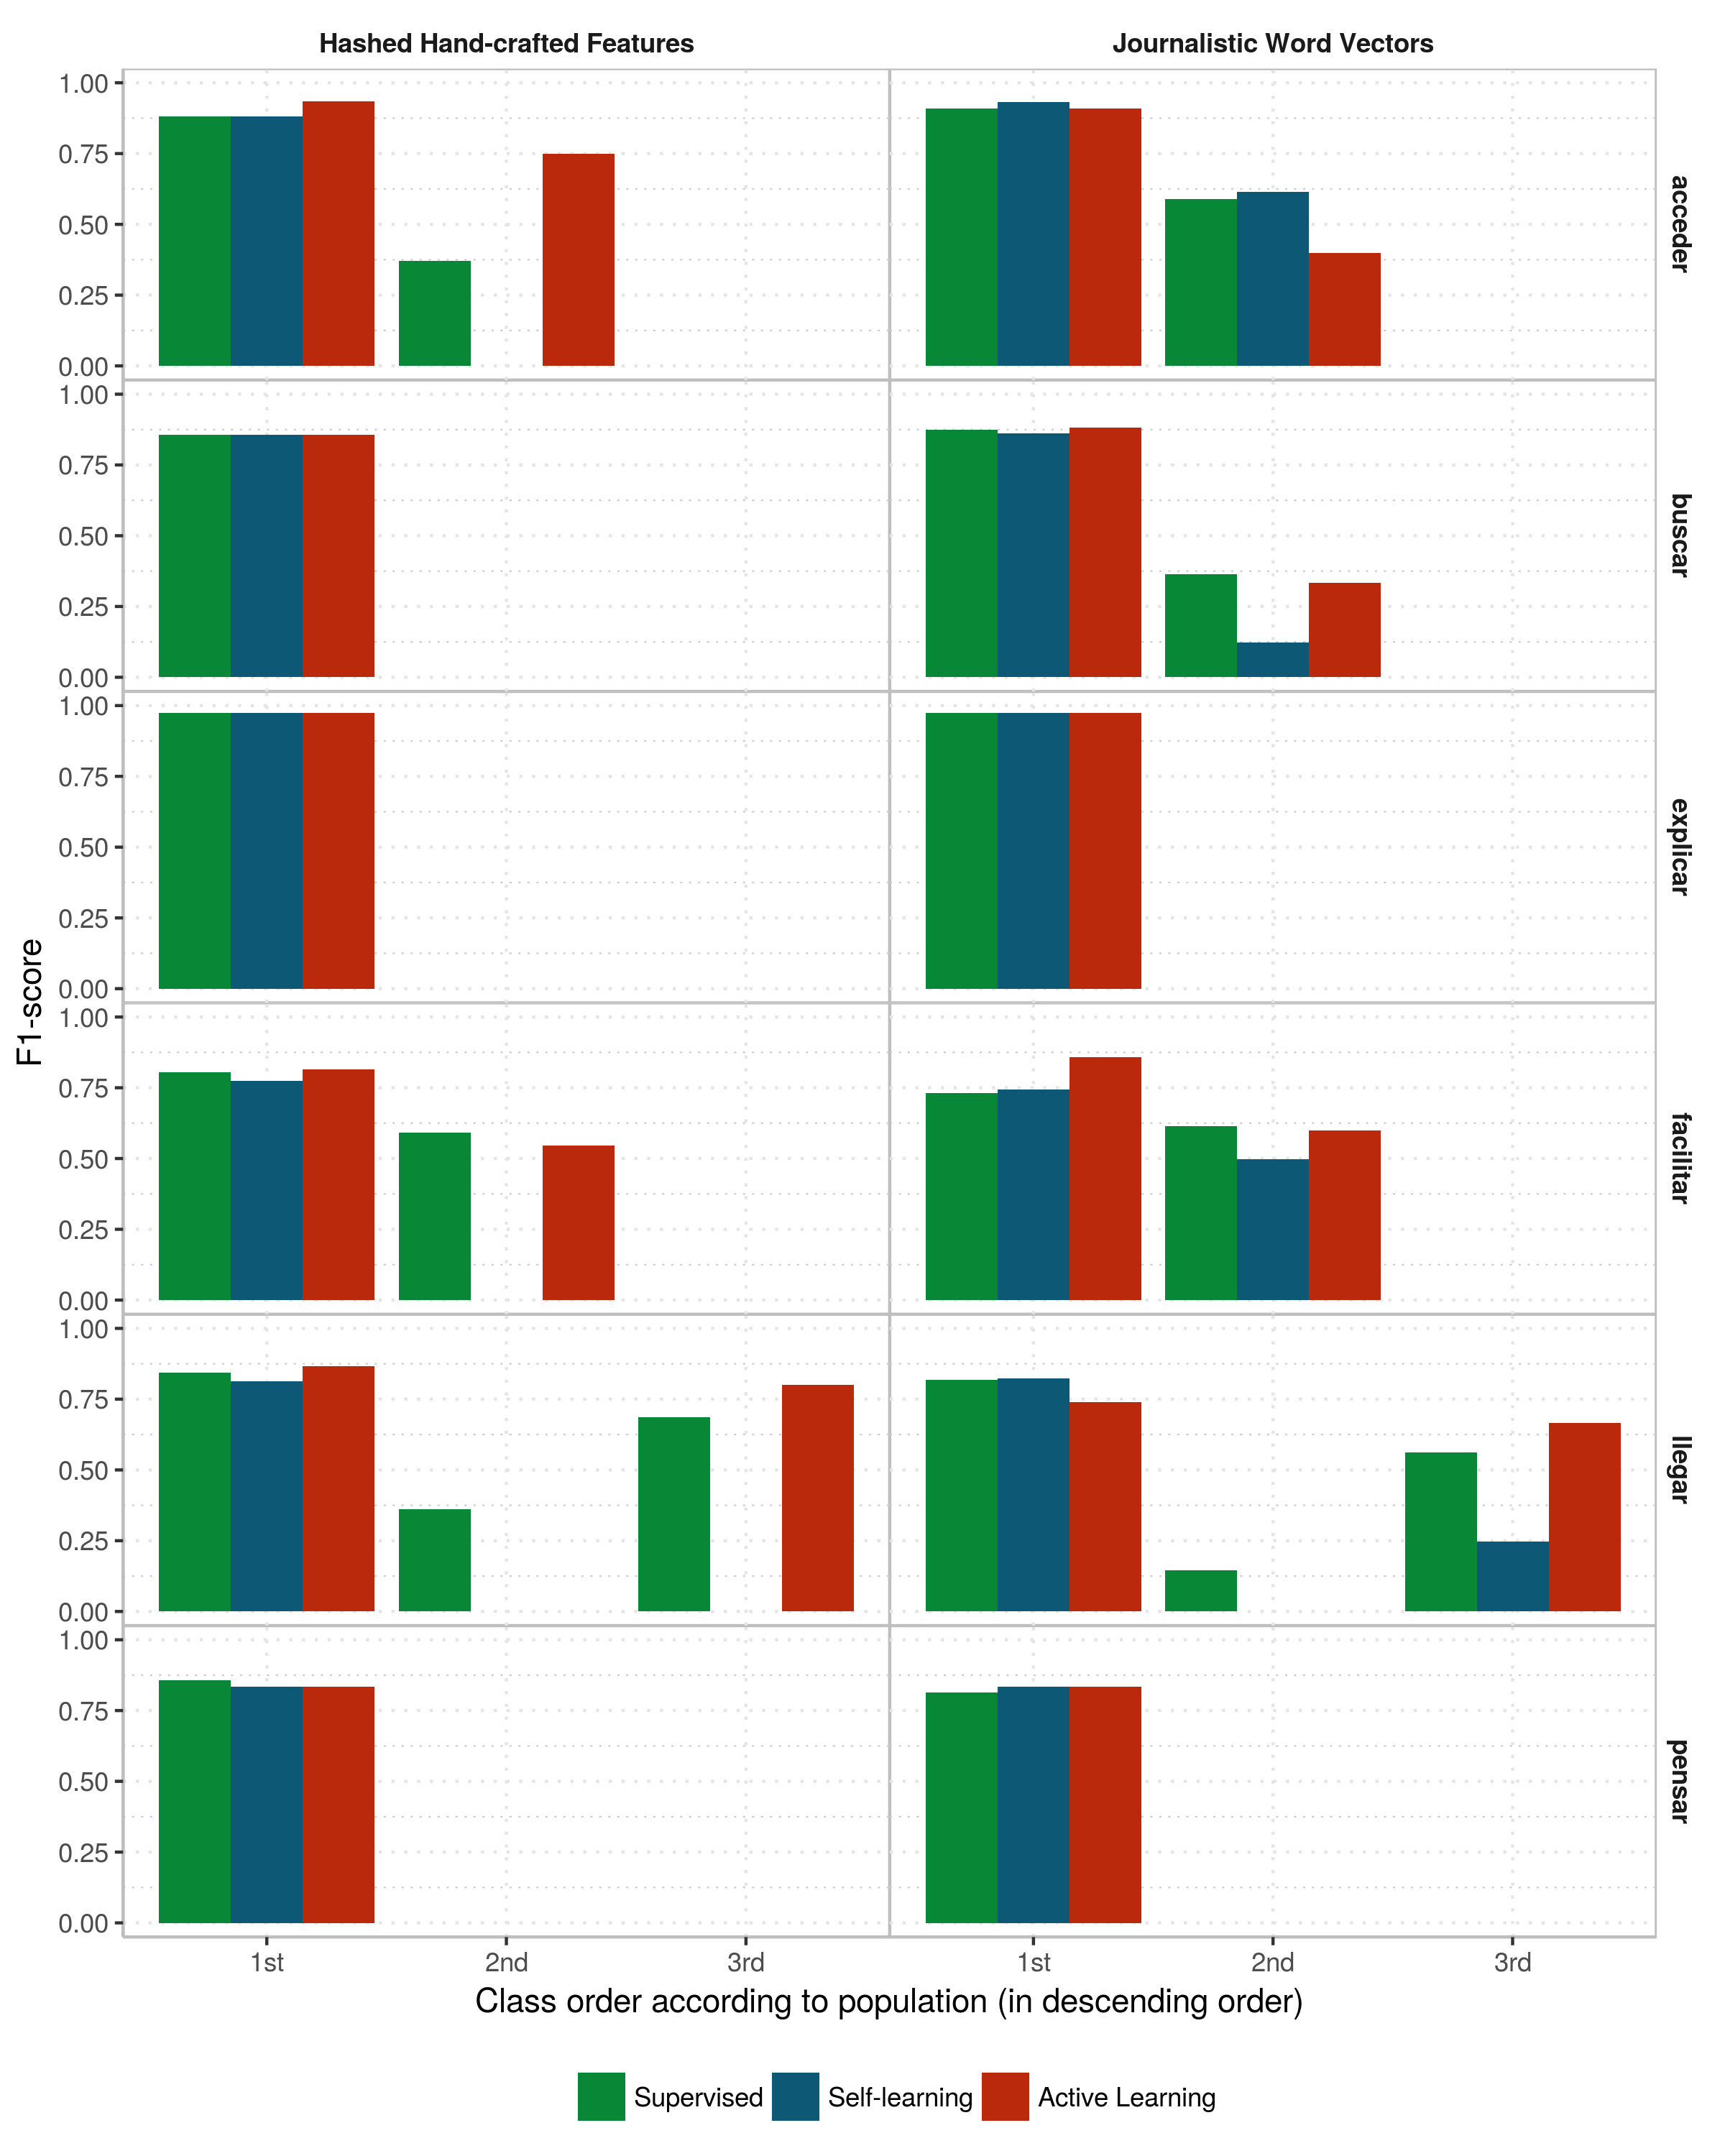
\includegraphics[height=0.9\textheight,width=\textwidth,keepaspectratio]
    {plots/active/per_sense_fscore}
  \caption{Comparison of macro and weighted average F1-score for supervised,
  self-learning and active learning}
  \label{fig:active:performance}
\end{figure}

Figure \ref{fig:active:performance} shows the F1-score macro and weighted
average for supervised, self-learning and active learning over the test
dataset. In this case, ``supervised'' is the evaluation of the model in the
initial iteration of any of the joint learning algorithms (as it is the same
for both, i.e. only using the manually labeled data). The self-learning/active
learning bars represent the performance of the model over the held-out test
dataset after finishing the iterations of the corresponding algorithm. The
structure of the graphic is as follows:

\begin{itemize}
  \item Each row shows the results for a token lemma: ``acceder'', ``buscar'',
    ``explicar'', ``facilitar'', ``llegar'', and ``pensar''.
  \item Each column stands for a feature representation: hand-crafted hashed
    features and journalistic word vectors.
  \item Each group of bars in each plot represents the class (i.e. sense) for
    that lemma. These are ordered according to number of occurrences of the
    class in the dataset.
  \item Each bar plot in a different color inside a group represents the
    algorithm: supervised (i.e. evaluation moment of the initial iteration),
    self-learning (i.e. evaluation moment of the final iteration after
    self-learning finishes), and active learning (i.e. evaluation moment of the
    final iteration after active learning finishes).
  \item The height of the bar represents the value of the F1-score per each
    class.
\end{itemize}

Recall again that only the last two rows of the graphic represent lemmas with 3
senses (i.e. ``llegar'' and ``pensar''). The first four lemmas can at most show
results for two senses.

In general, active learning performs better than self-learning and even better
than supervised in some cases for both the most frequent class and the less
frequent classes. It might be that active learning performed better than
supervised learning simply because the amount of annotated examples increases.
However, the amount of annotated examples also increases for self-learning, but
it does not impact in the performance. This is a clear sign that the selection
of examples to give to the oracle to annotate is in the right track, because it
does have a visible impact in the performance of the resulting model, beyond
the mere increment in the number of annotated examples.

Once again, like in the previous chapter, word embeddings still show better
overall performance than hand-crafted features: minority senses are better
represented, without an important loss of performance in majority senses. In
combination with active learning, word embeddings become particularly useful,
as they properly characterize minority senses. 

Now that I have a base comparison of the two algorithms I have strong evidence
that active learning is better for the performance of the model. To check why
this is the case I will look further into the hypotheses.

\subsection{Hypothesis \ref{hyp:active:1}}\label{sec:active:hyp:1}

This section tests Hypothesis \ref{hyp:active:1}. The hypothesis states that
the representativity of each class's population in the training dataset is
maintained through all the algorithm iterations. Recall that for the
self-learning algorithm I found evidence to accept Hypothesis
\ref{hyp:self-learning:6}, which states the opposite of Hypothesis
\ref{hyp:active:1}. 

More precisely, I established that the fact that self-learning was not
representing all classes properly was the cause for the self-learning degrading
the performance of the less frequent classes, as stated in Hypothesis
\ref{hyp:self-learning:5} in the previous chapter. As I saw in the previous
section, this is not the case for active learning, since it does improve on the
performance of classes other than the most frequent one.

I show the results for Hypothesis \ref{hyp:active:1} to assess whether the
reason behind the improvement in performance is effectively a better
representation of the minority classes with the active learning algorithm.

To test the hypothesis I measure the results obtained after doing Experiment
\ref{exp:active:2} which records the number of instances each of the classes
has in the training dataset after each active learning iteration.

Once again, as in the previous chapter, to visualize these results I use two
techniques to show what, for me, is relevant on the checking of the Hypothesis:
the proportional count of the number of instances per class along the
iterations, and the proportional number of instances added for each class per
iteration. These two results will allow to accept Hypothesis
\ref{hyp:active:1}.

\subsubsection{Classes' population distribution across iterations}

\begin{figure}[htb!]
  \centering
  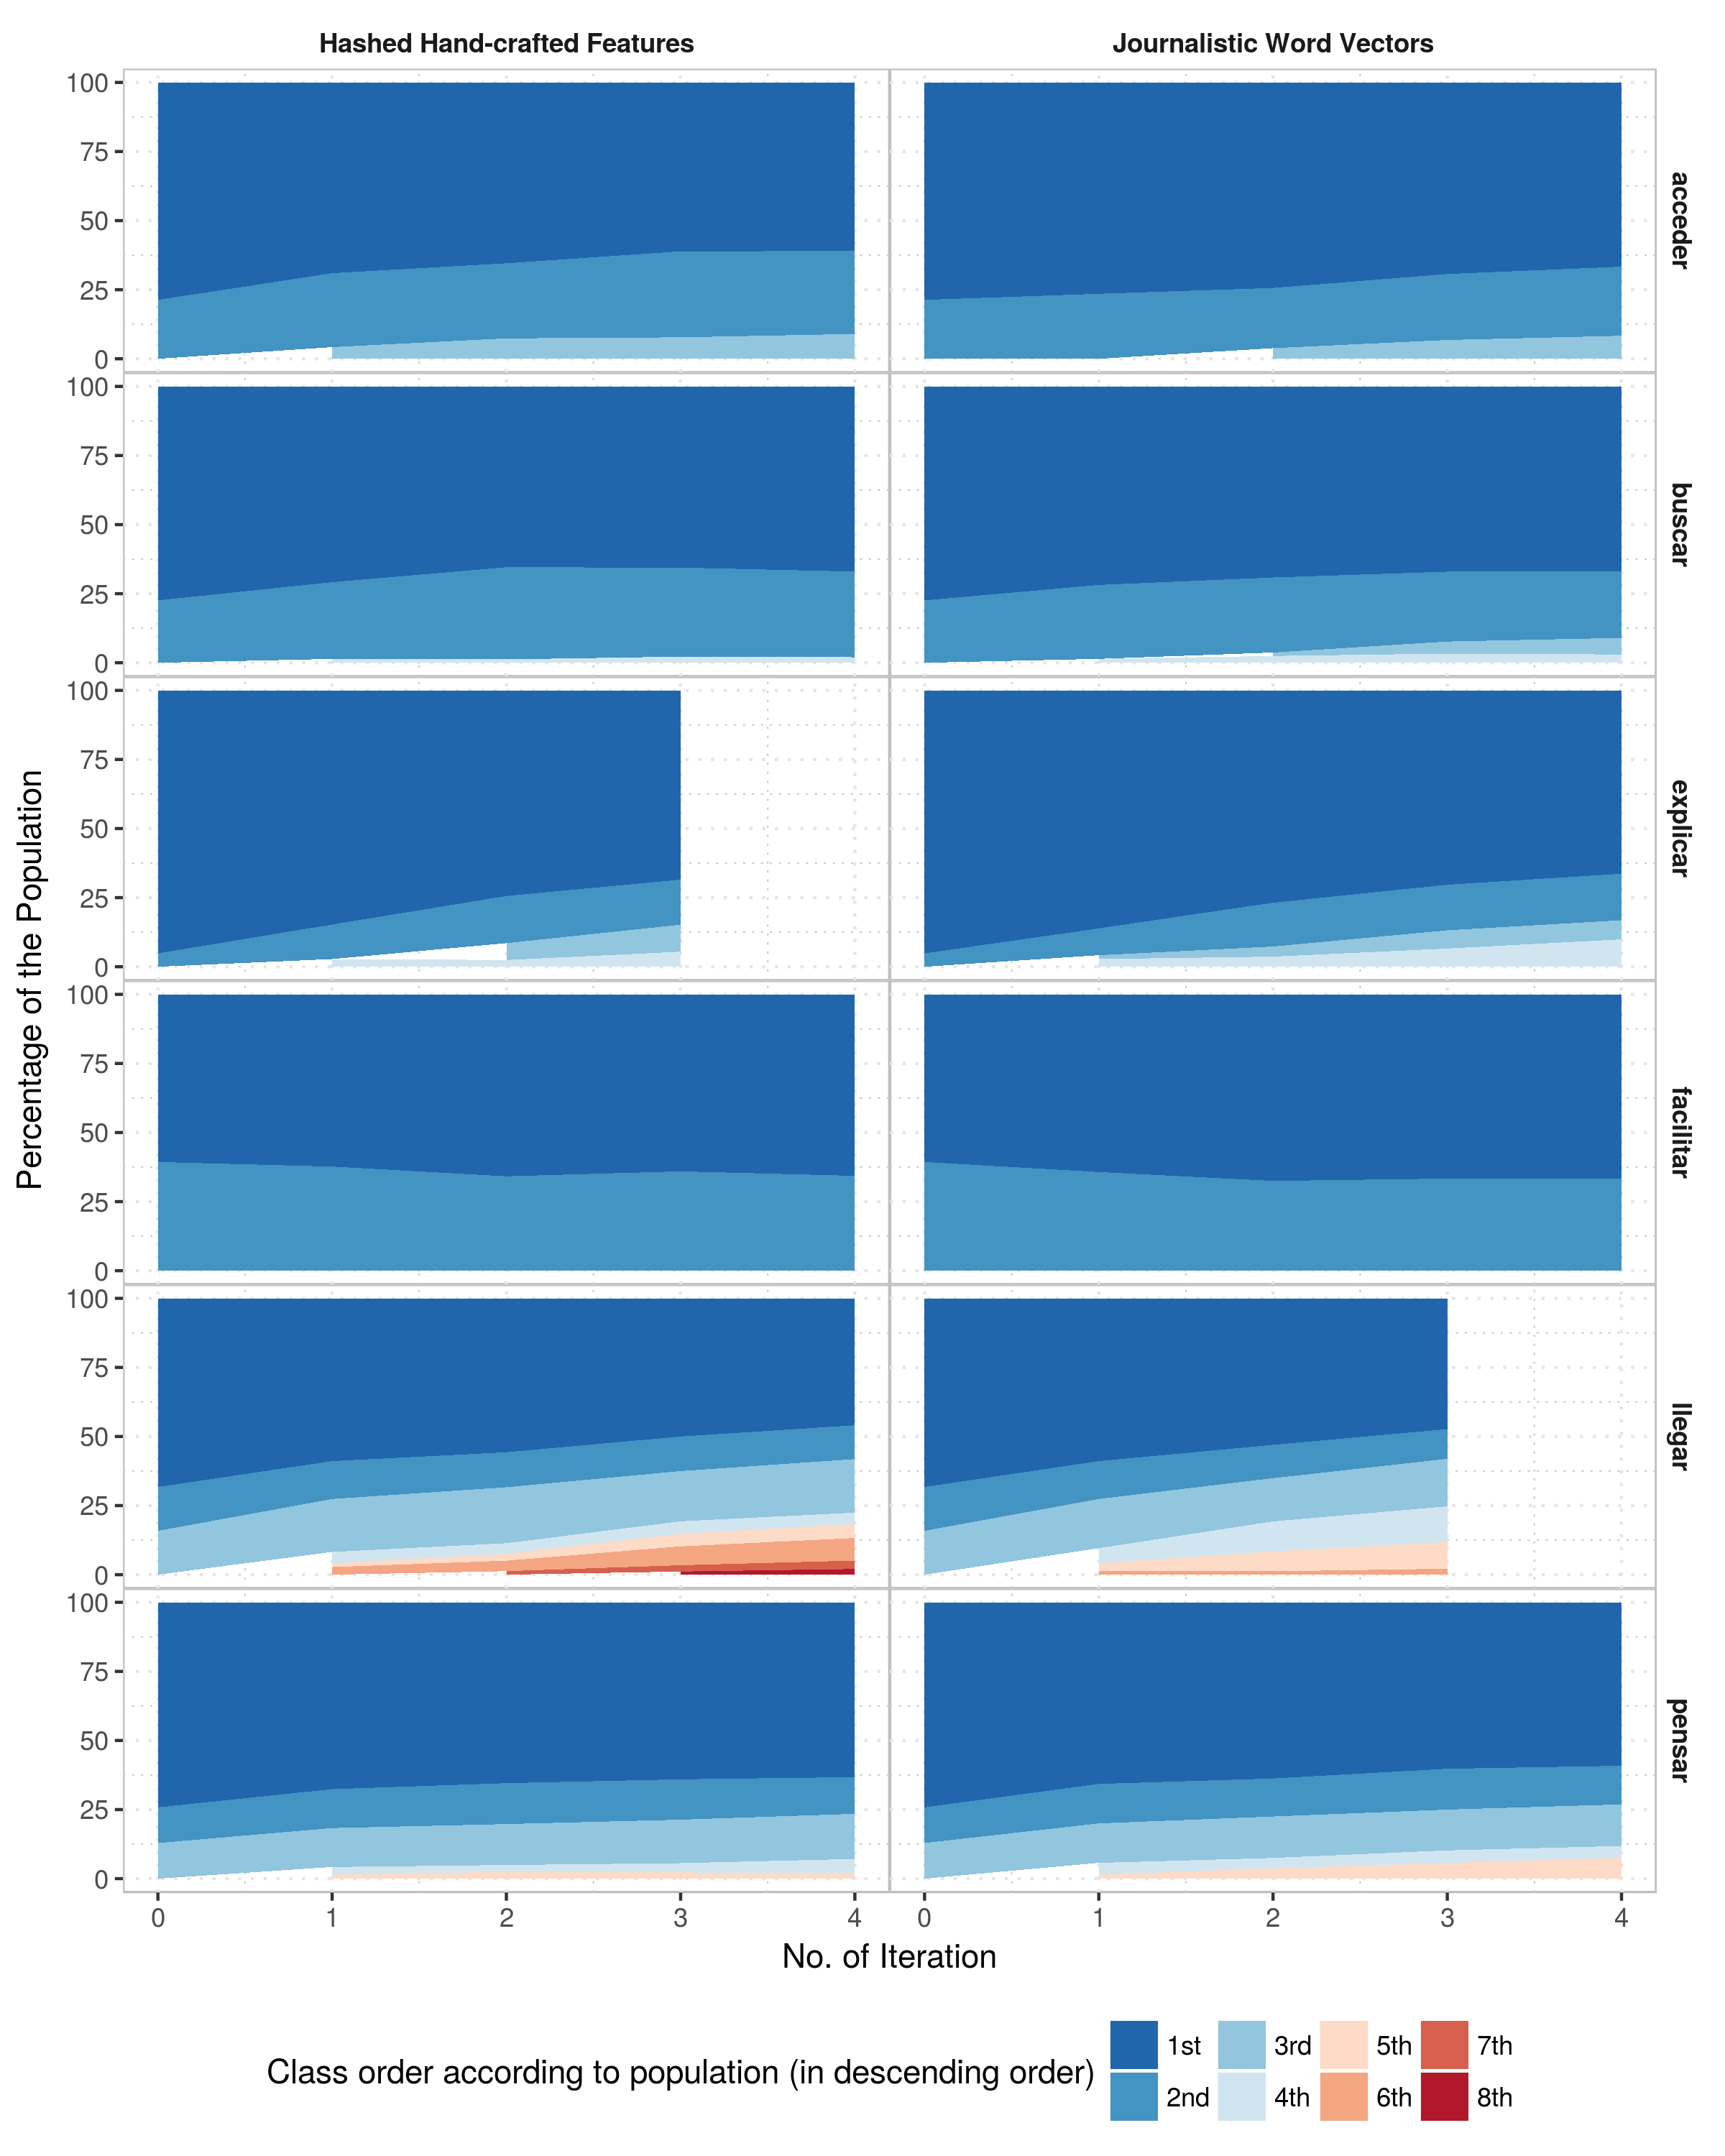
\includegraphics[height=0.9\textheight,width=\textwidth,keepaspectratio]
    {plots/active/population_distribution}
  \caption{Distribution of the classes' population across active learning
  algorithm's iteration as a proportion of the whole training dataset}
  \label{fig:active:population_distribution}
\end{figure}

Figure \ref{fig:active:population_distribution} shows the distribution of the
population of the classes across the active learning iterations. Each class's
population is represented as the proportion of the total number of examples in
the training dataset for that iteration. The plot is a stacked area plot that
follows this structure:

\begin{itemize}
  \item Each row shows the results for a token lemma: ``acceder'', ``buscar'',
    ``explicar'', ``facilitar'', ``llegar'', and ``pensar''.
  \item Each column stands for a feature representation: hand-crafted hashed
    features and journalistic word vectors.
  \item The x-coordinate represents the iteration in the self-learning
    algorithm.
  \item The y-coordinate represents the percentage of population.
  \item Each area of a different color represents the proportion of examples
    for each of the classes in the dataset. The classes again are ordered
    according to number of examples in the original supervised dataset.
\end{itemize}

The first thing to notice from the figure, specially compared to the similar
figure of the previous chapter, is the number of iterations. While for
self-learning iterations could go up to 100, for active learning I only did the
annotations for 4 iterations total (plus the initial iteration, which is
represented in the number 0). This is why I say that the work done for active
learning is mostly exploratory.

Note that there are two cases where the iterations are less: ``explicar'' (for
the hand-crafted features representation) and ``llegar'' (for the word
embeddings representation). In this cases the iteration finished before because
the stopping criterion of the validation error was met.

The second noticeable thing in the figure is the increase in the number of
classes that occur as the iterations advance. This is a result of what I
explained before: the algorithm selects those instances on which it does not
have enough information, which are generally those that are not part of the
original supervised corpus. This is a marked difference with self-learning: in
active learning the less frequent classes also grow in number of examples
through the iterations, not only the most frequent one.

\subsubsection{Population added per sense per iteration}

\begin{figure}[htb!]
  \centering
  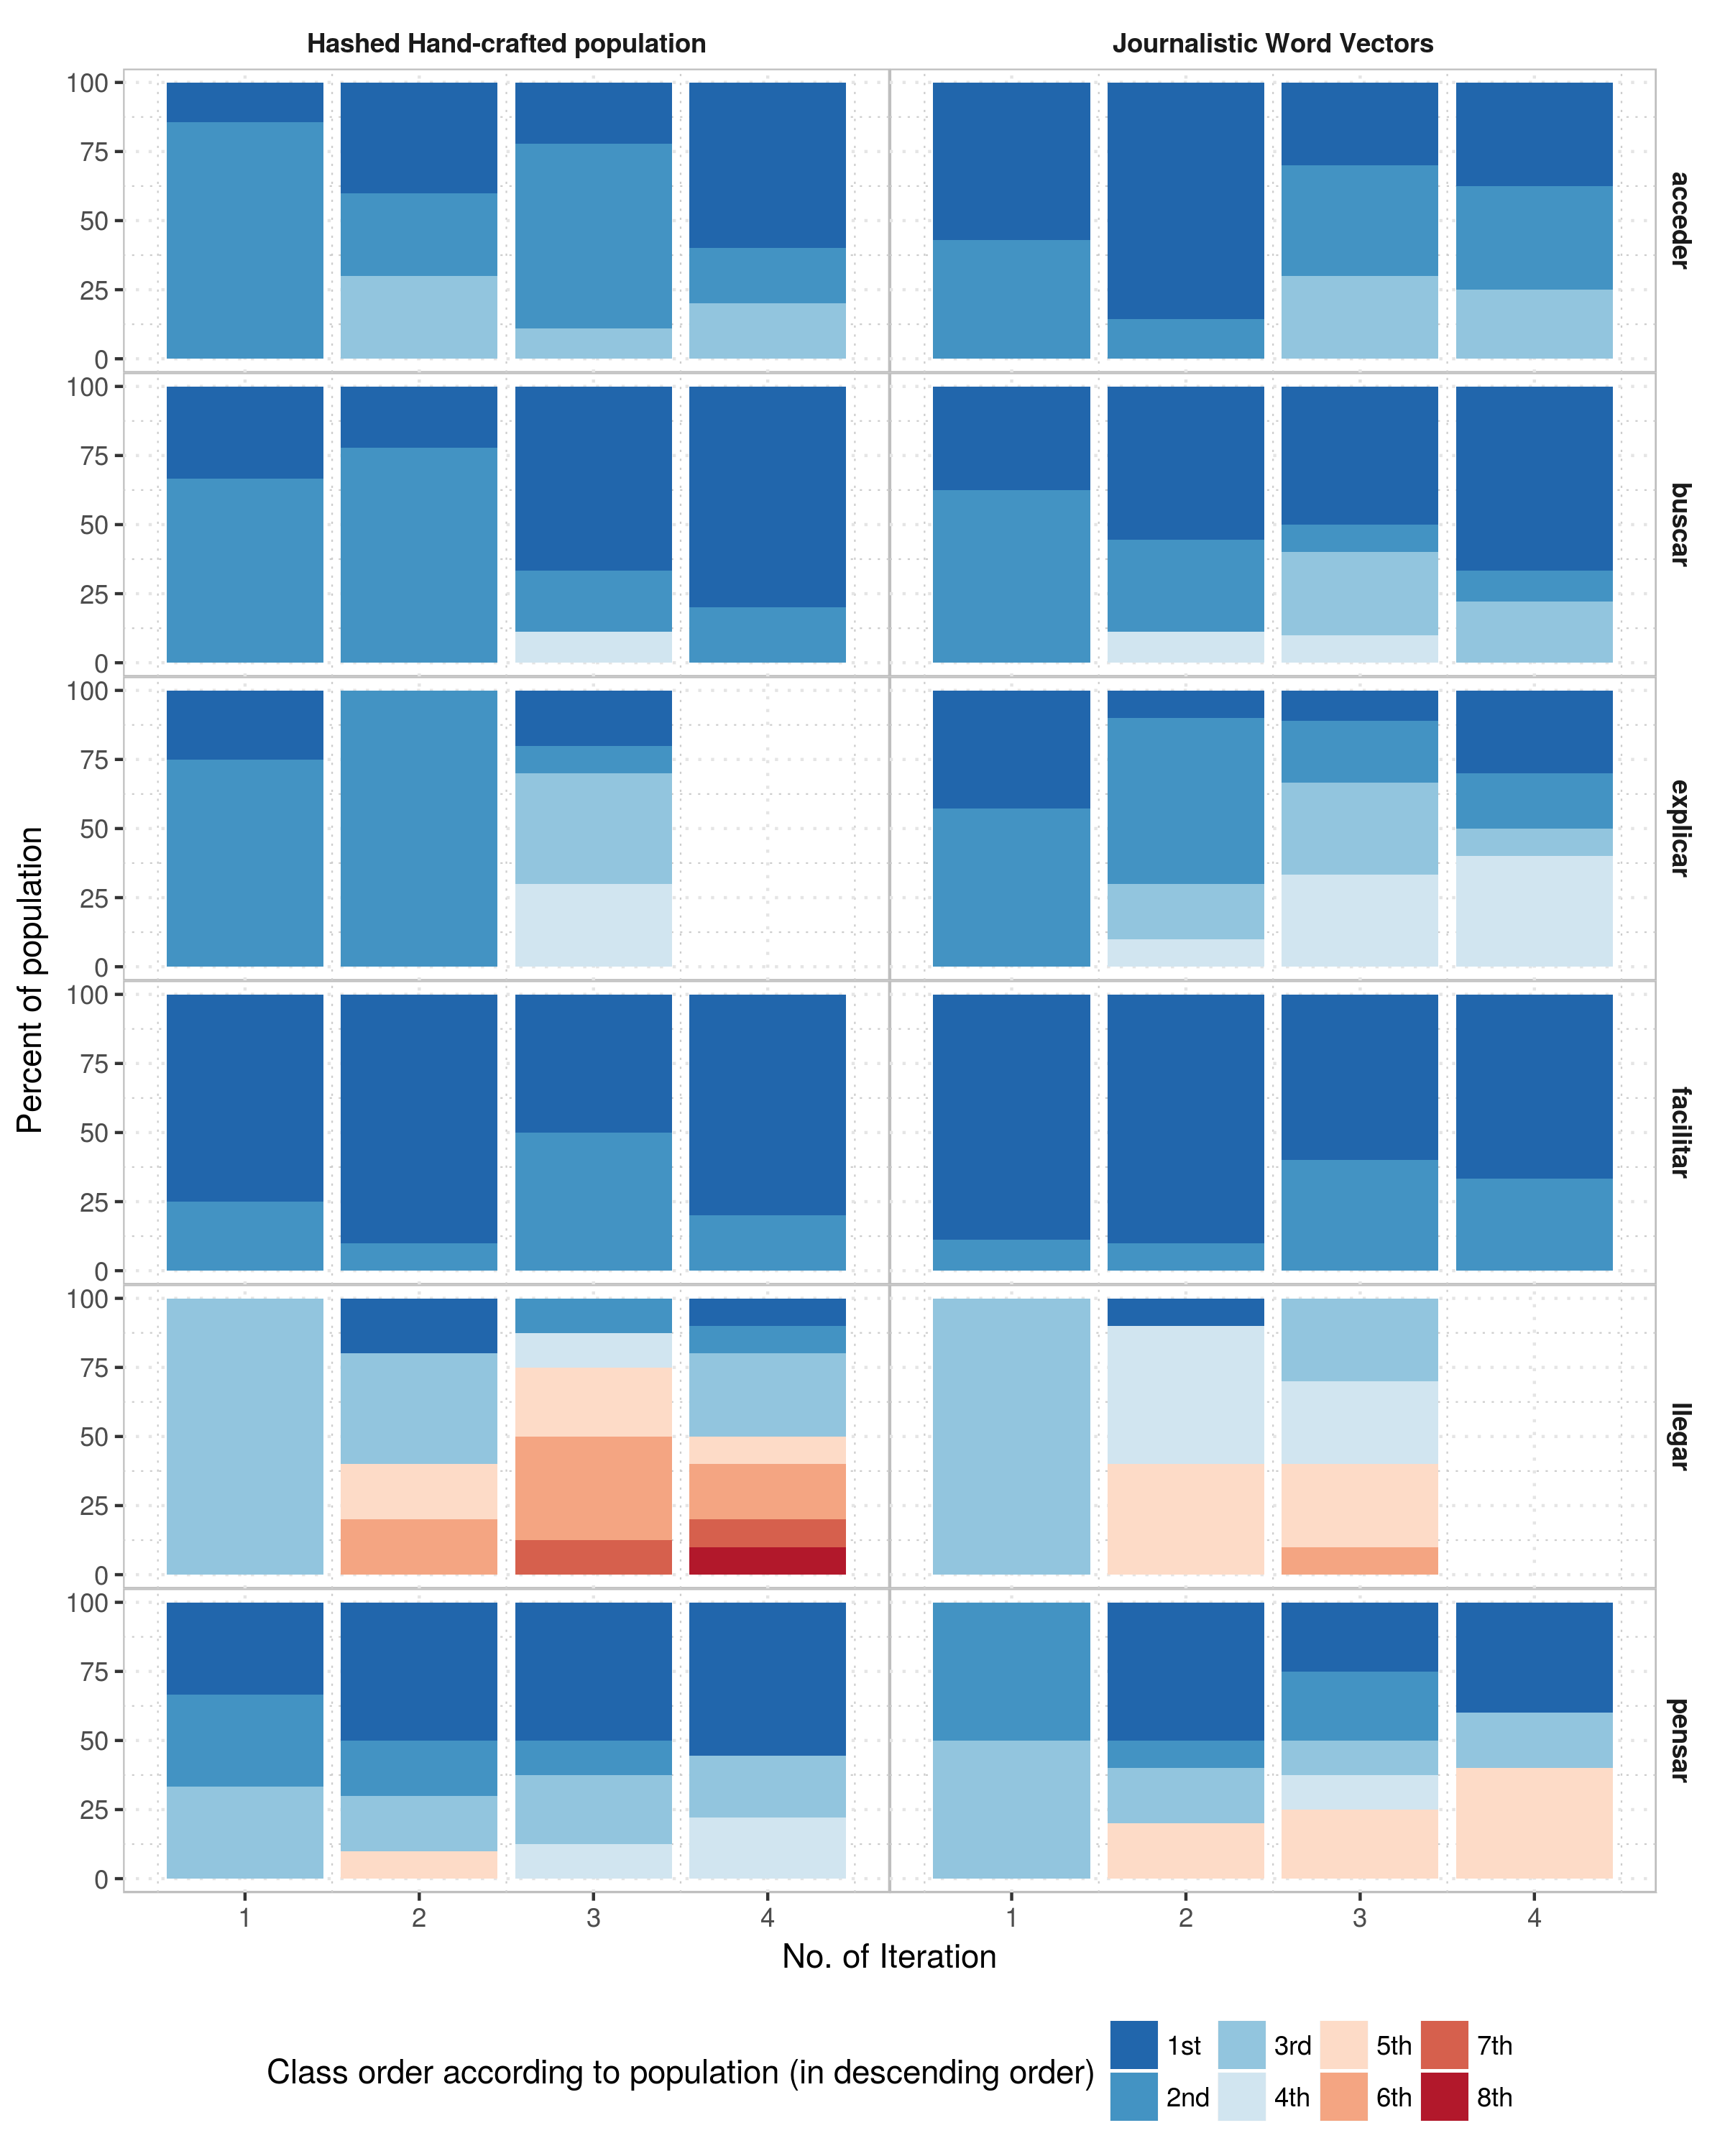
\includegraphics[height=0.9\textheight,width=\textwidth,keepaspectratio]
    {plots/active/population_add_per_class}
  \caption{Population added per sense on each iteration of active learning as a
  proportional count of all the examples added in that iteration}
  \label{fig:active:population_add_per_class}
\end{figure}

Figure \ref{fig:active:population_add_per_class} shows the proportion of
examples added per class on each iteration. It is a stacked bar plot where each
bar represents the total examples added in the iteration split by the
proportion of classes automatically annotated as such. The structure of the
plot is the following:

\begin{itemize}
  \item Each row shows the results for a token lemma: ``acceder'', ``buscar'',
    ``explicar'', ``facilitar'', ``llegar'', and ``pensar''.
  \item Each column stands for a feature representation: hand-crafted hashed
    features and journalistic word vectors.
  \item The x-coordinate represents the iteration in the self-learning
    algorithm.
  \item The y-coordinate represents the percentage of examples automatically
    annotated and added to the model.
  \item Each bar plot represents the distribution of the examples added in
    the iteration. Each color of the stacked bar represents the class
    which the examples were annotated.
\end{itemize}

In the figure there is a better view of what is happening along each iteration.
In general, the less frequent classes add more examples than the most frequent
class through iterations. This is a consequence of using uncertainty sampling,
which selects those classes near the decision border of the classifier.

In general, word embeddings are more uniform when adding examples of many
different classes. The consequence of this, I can hypothesize, is that for
hand-crafted features, and as a consequence of the low generalization they
have, the classifier is more certain about the most frequent class and thus
when applying the uncertainty sampling technique it choses mostly examples of
the less frequent classes. Word embeddings, on the other hand, have better
generalization from the start, thus when sampling elements with uncertainty it
can have low certainty also for some of the examples of the most frequent
class.

In any case, from these results I have enough evidence to support Hypothesis
\ref{hyp:active:1} which states that the distribution of the different classes
through the active learning algorithm iterations is maintained.

\subsection{Hypothesis \ref{hyp:active:2}}\label{sec:active:hyp:2}

I follow up with the test of Hypothesis \ref{hyp:active:2}. Recall that the
hypothesis states the active learning algorithm adds more information with the
examples it adds to the model in comparison to self-learning. This is a
consequence of the examples added being of classes the model has already less
information about due to the uncertainty sampling technique.

To test the Hypothesis I measure the results of Experiment \ref{exp:active:3},
which records the number of times a feature appears with a class. However, what
I am mostly interested about in this occasion is the total number of features
added per iteration of both self-learning and active learning algorithms. These
results are measured by Metric \ref{met:6} which is the normalized count of
features added in an iteration by the examples added in the same iteration.
The reason to use this measure instead of the raw count is because it is clear
that the number of features for self-learning will be higher than for active
learning since the number of examples that self-learning annotates in each
iteration is of a magnitude greater than active learning. However, what the
Hypothesis states, and what I am interested about, is whether these fewer
examples of the active learning algorithm actually add more information than
the self-learning algorithm.

\begin{figure}[htb!]
  \centering
  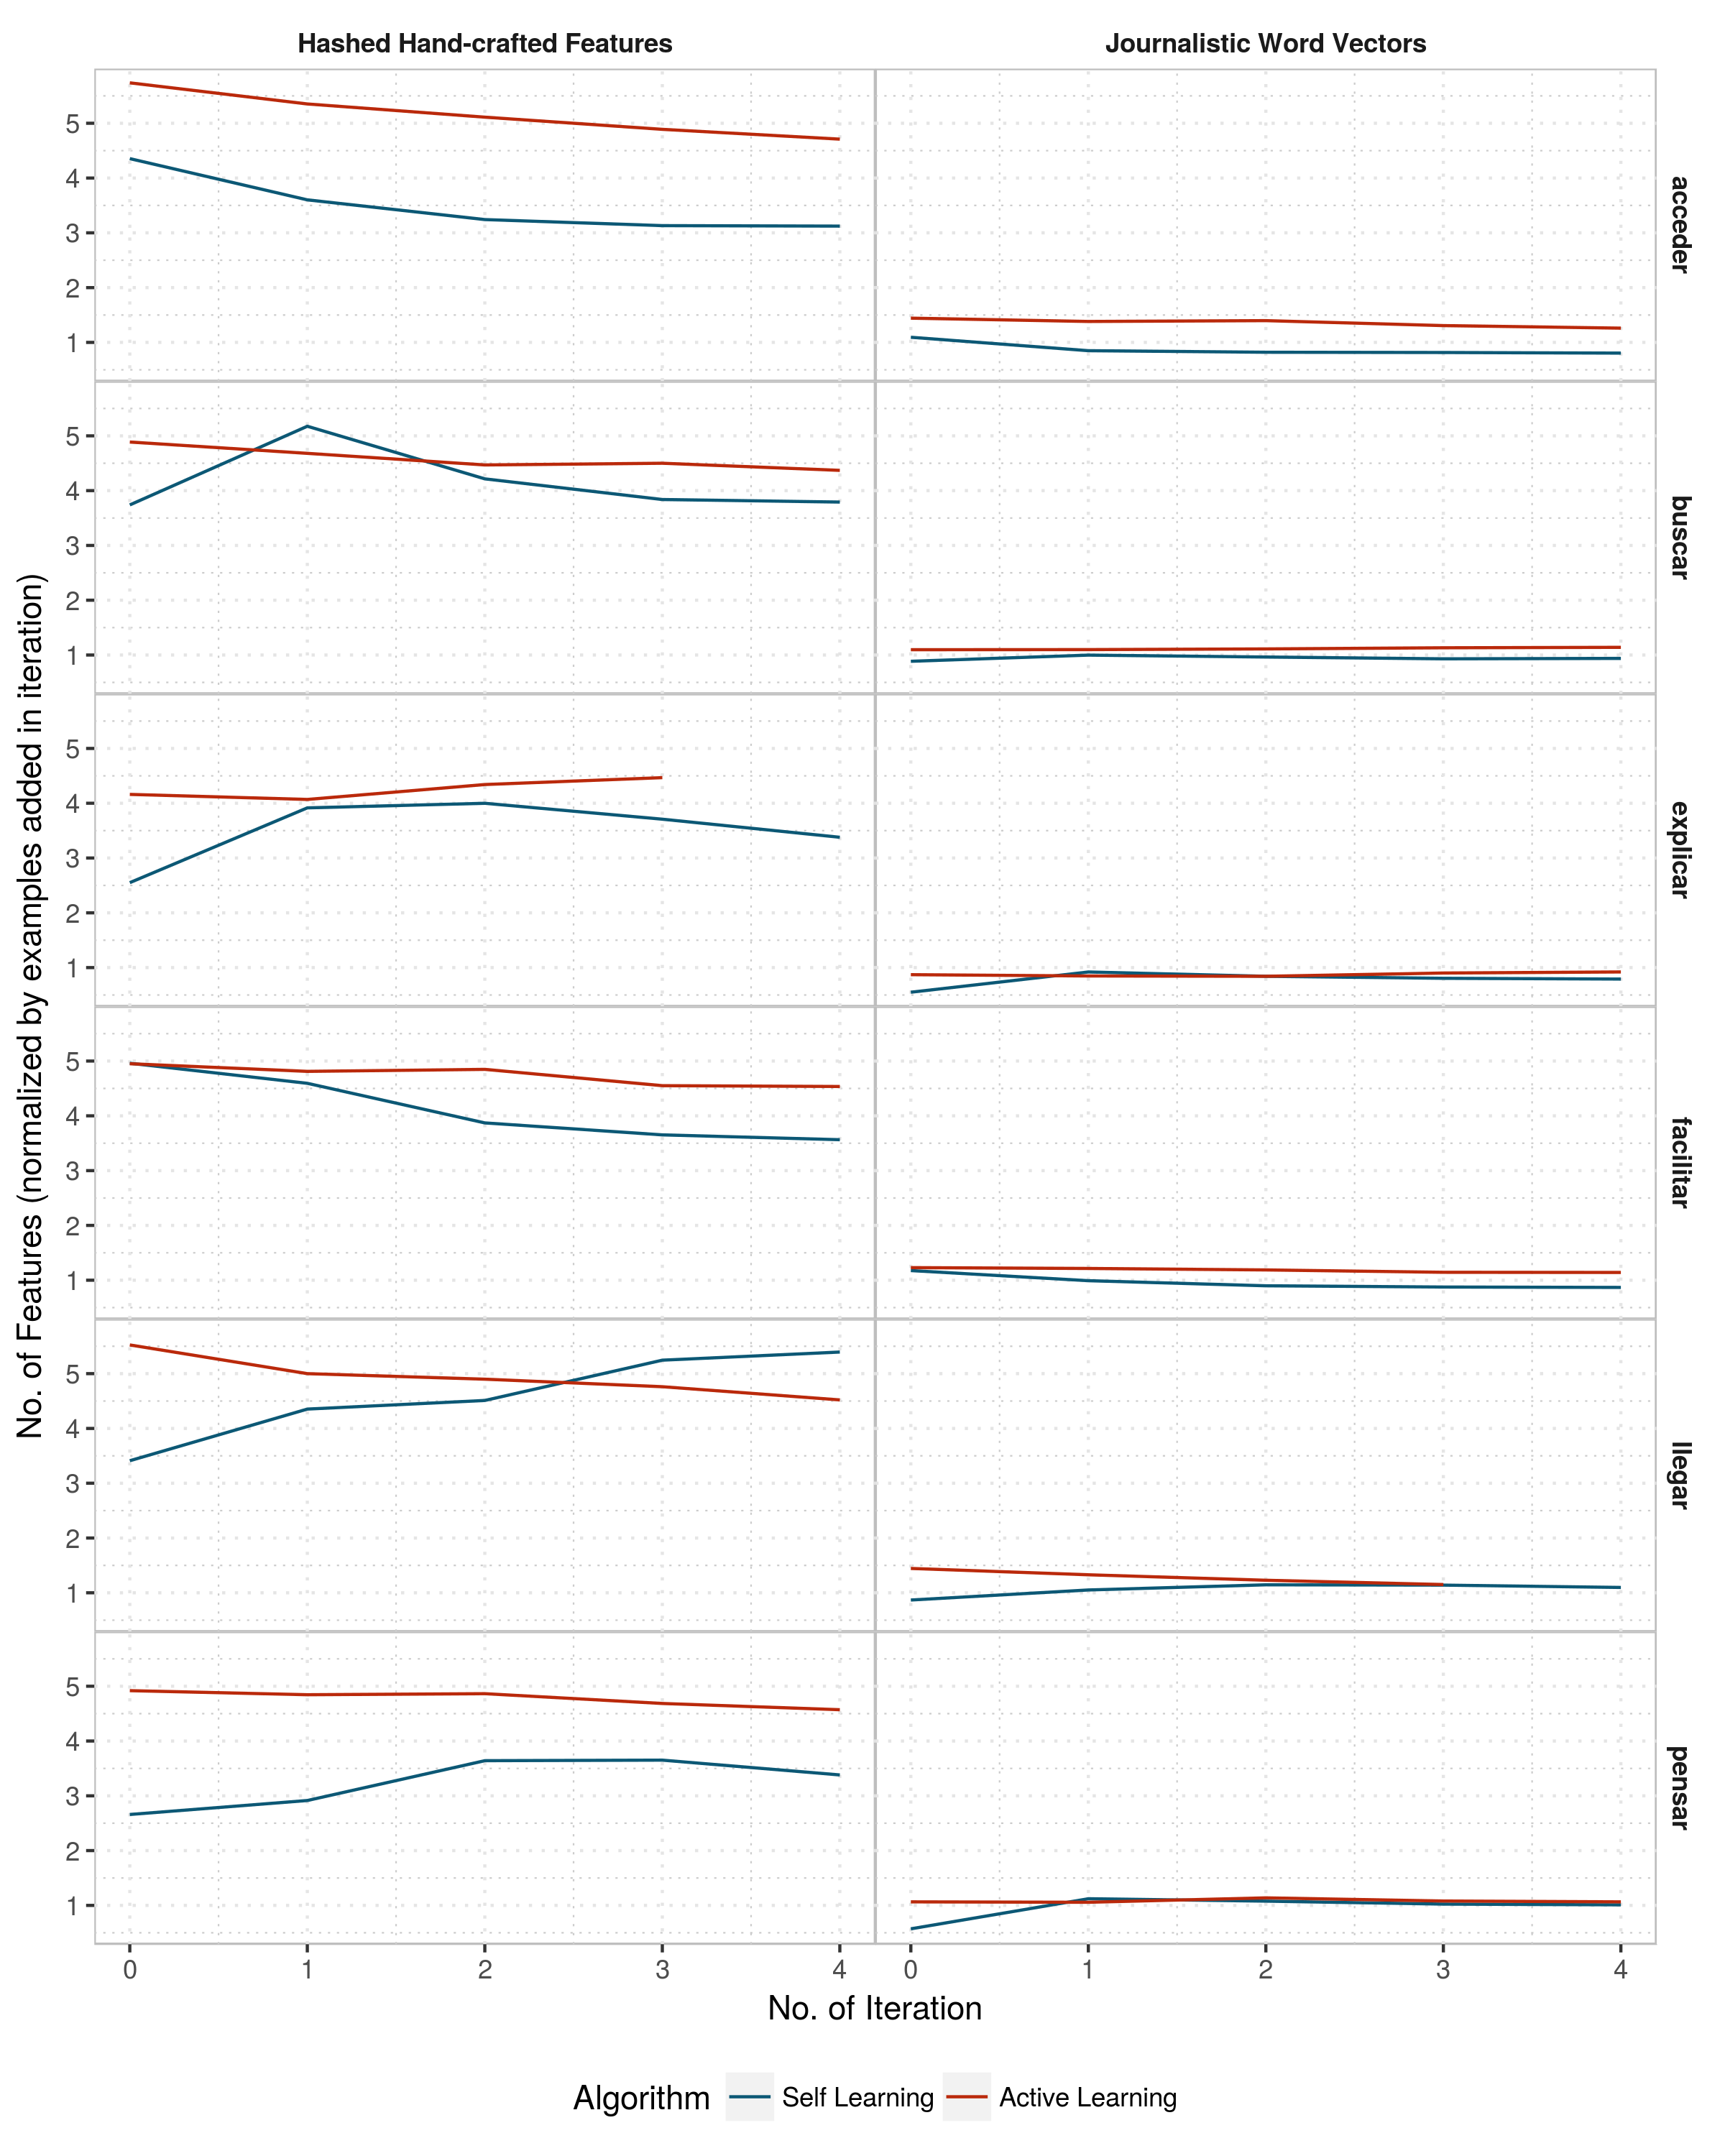
\includegraphics[height=0.9\textheight,width=\textwidth,keepaspectratio]
    {plots/active/feature_growth_comparison}
  \caption{Number of features added in each iteration of both self-learning
  and active learning. The features are normalized by the number of examples
  added in the iteration}
  \label{fig:active:feature_growth_comparison}
\end{figure}

Figure \ref{fig:active:feature_growth_comparison} shows the amount of features
added in each iteration of both self-learning and active learning normalized by
the amount of examples added. The structure of the graphic is as follows:

\begin{itemize}
  \item Each row shows the results for a token lemma: ``acceder'', ``buscar'',
    ``explicar'', ``facilitar'', ``llegar'', and ``pensar''.
  \item Each column stands for a feature representation: hand-crafted hashed
    features and journalistic word vectors.
  \item The x-coordinate axis represents the iteration number in the
    self-learning algorithm.
  \item The y-coordinate axis represents the normalized count of unique
    features by the number of examples added.
  \item Each line represents the number of features and the different colors
    represents the algorithm: self-learning and active learning.
\end{itemize}

The tendency shown in Figure \ref{fig:active:feature_growth_comparison} is
clear enough. Active learning is adding more information to the model by adding
more features per examples in comparison to self-learning. This is clearly a
consequence of active learning adding examples of less frequent classes in
contrast to self-learning as I showed in the previous Hypothesis's results.
Moreover, active learning is adding examples of classes that are non-existent
for self-learning since the classes are not part of the initial seed model.

For active learning, the most frequent class, which contains most of the
features in the initial model, is not the only one to grow in each iteration
(in fact, sometimes it is the one with the lowest number of examples added in
an iteration). Thus that class is not overtaking all the features added per
iteration. Then, when instances of classes with less occurrences are added the
data enriches more the model initial model. This can also be seen by inspecting
the PMI of the features and the classes, as in the next section.

\subsubsection{Features PMI}

There is another view for the results of Experiment \ref{exp:active:3}, that is
the one measured by the PMI defined in Metric \ref{met:5}, which associates the
features to the classes with a higher PMI and then gets the mean PMI per class.
In this section I show the results as measured by that metric and draw
conclusions regarding the Hypothesis.

\begin{figure}[htb!]
  \centering
  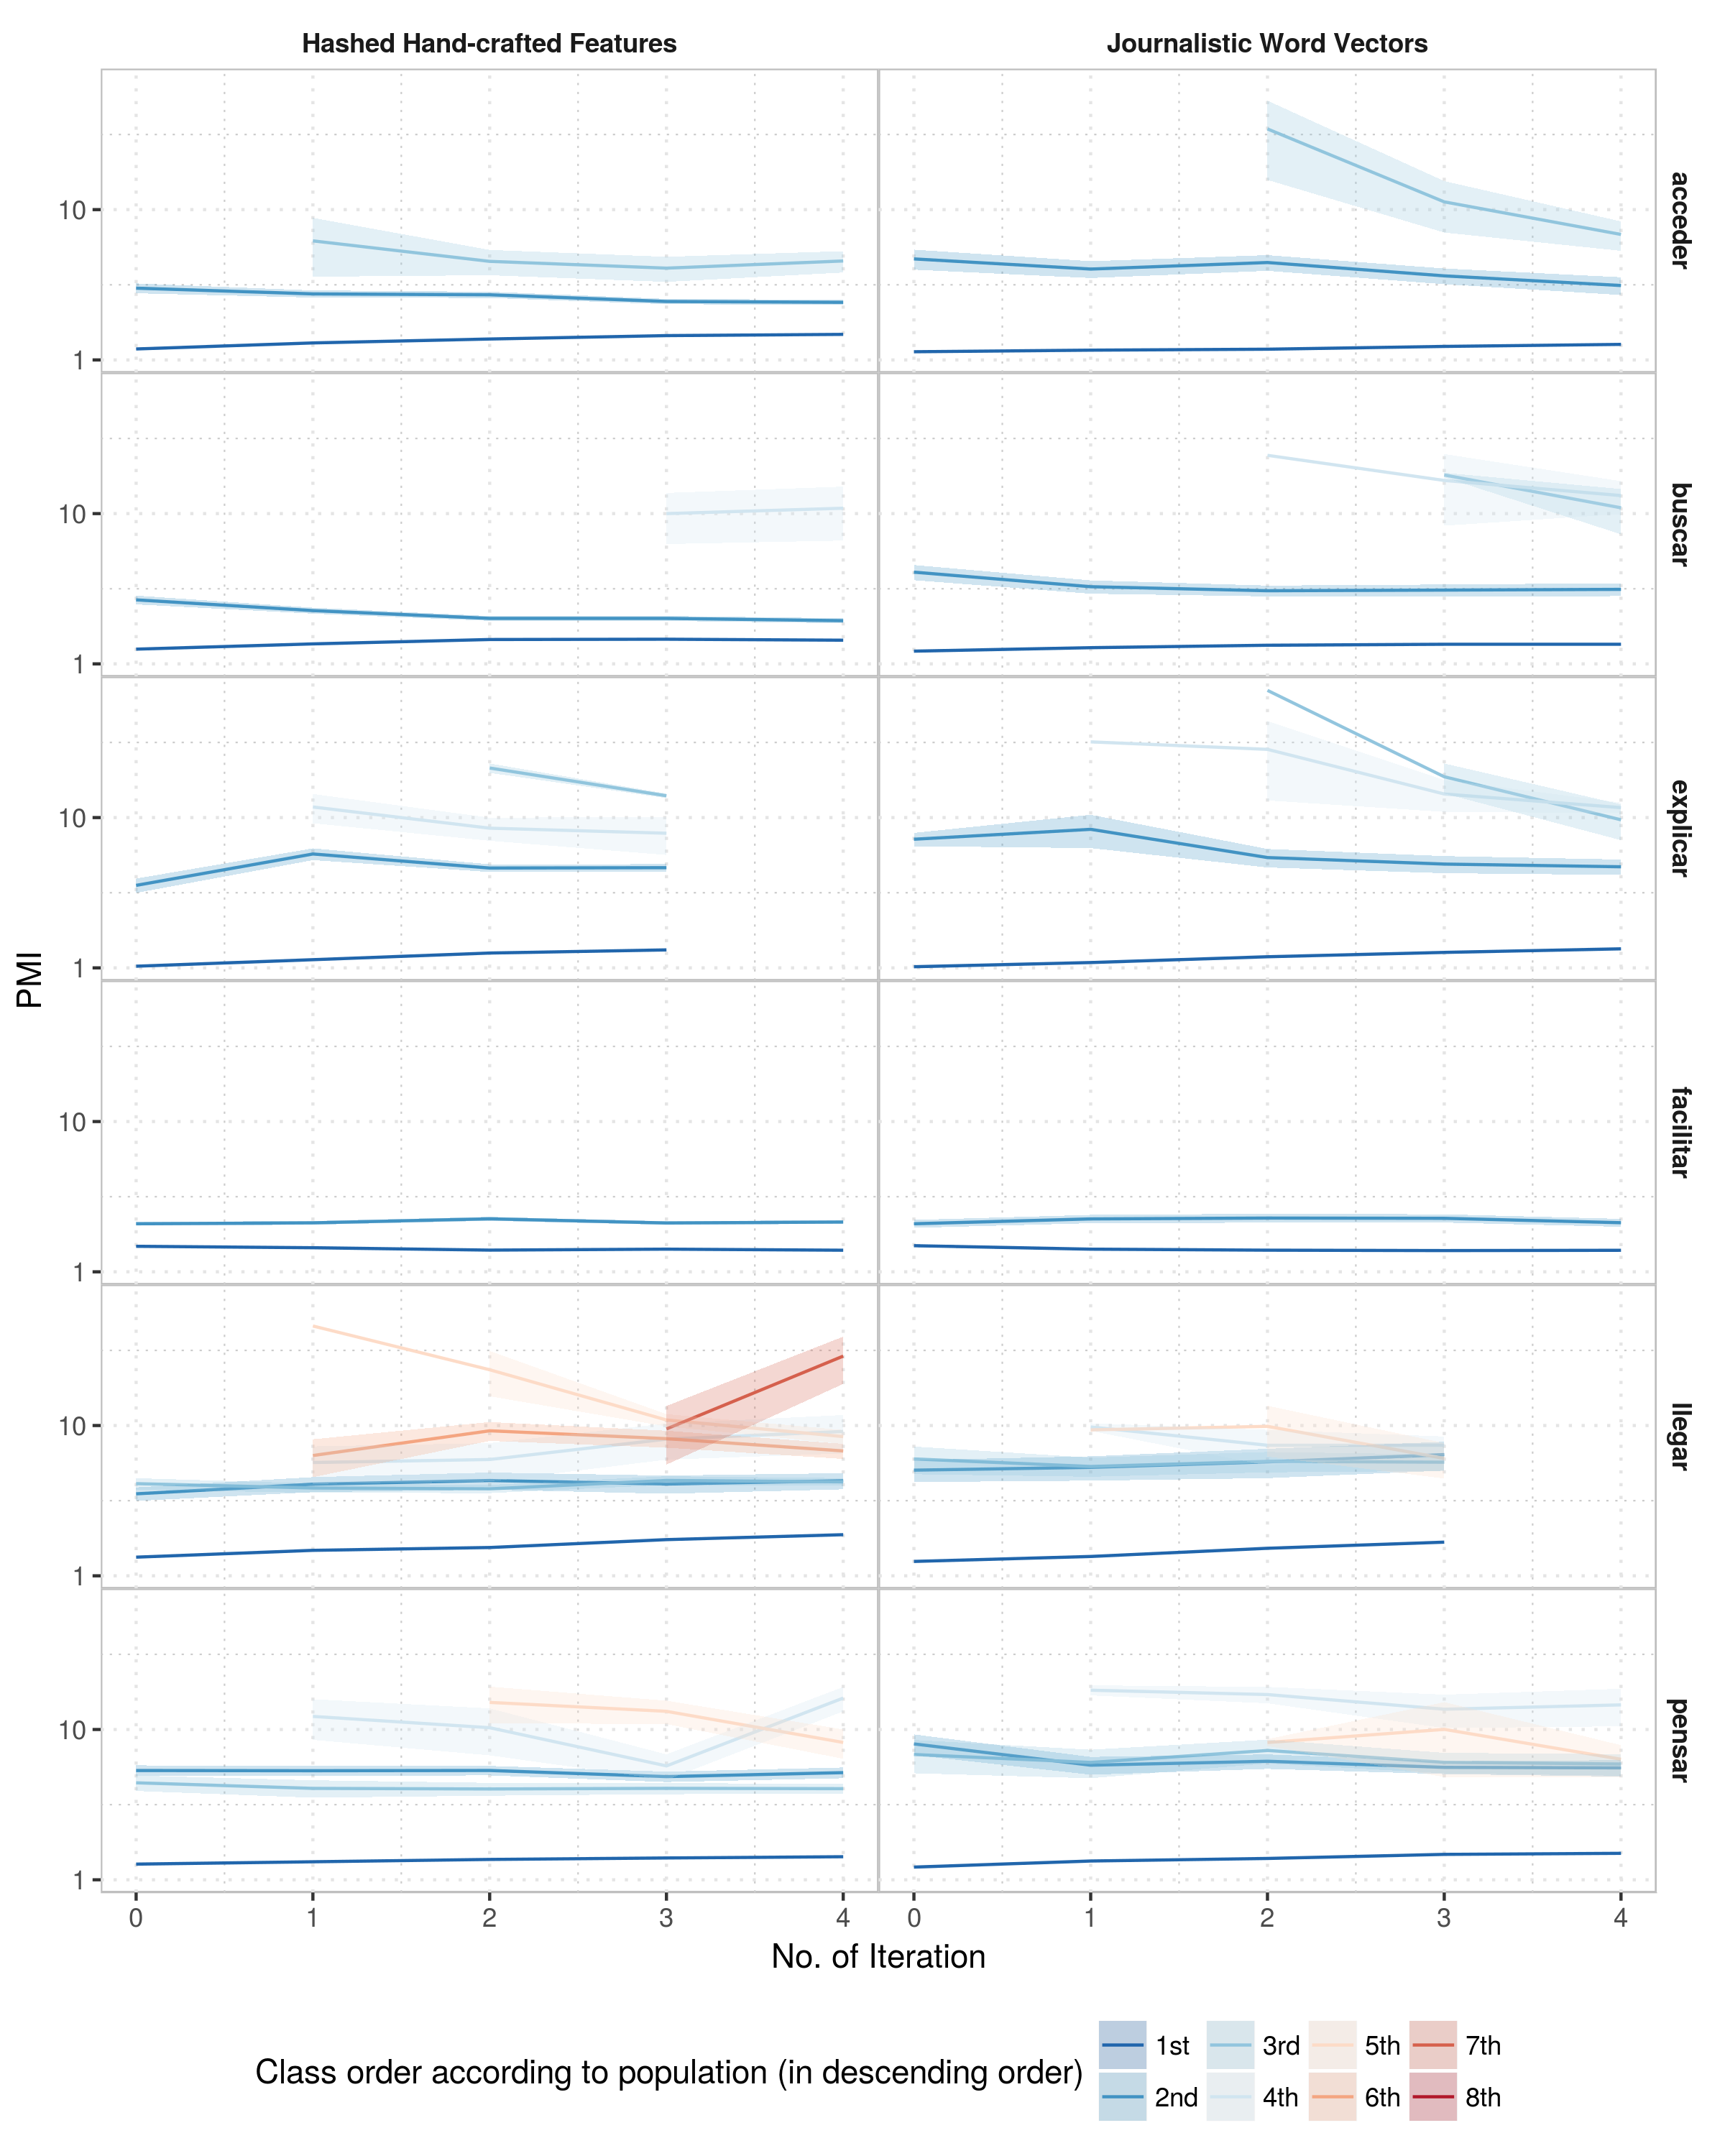
\includegraphics[height=0.9\textheight,width=\textwidth,keepaspectratio]
    {plots/active/features_pmi}
  \caption{Features pointwise mutual information with each of the classes
  across active learning iterations}
  \label{fig:active:pmi}
\end{figure}

Figure \ref{fig:active:pmi} displays the mean and standard error of the mean of
the pointwise mutual information between features and classes across the active
learning iterations. Recall that the metric associates features to the class it
has a larger PMI with. The figure shows a line plot with the following
structure:

\begin{itemize}
  \item Each row shows the results for a token lemma: ``acceder'', ``buscar'',
    ``explicar'', ``facilitar'', ``llegar'', and ``pensar''.
  \item Each column stands for a feature representation: hand-crafted hashed
    features and journalistic word vectors.
  \item The x-coordinate axis represents the iteration number in the
    self-learning algorithm.
  \item The y-coordinate axis represents the raw count of unique features in a
    logarithmic scale.
  \item Each color represents a class.
  \item The line of darker color in the middle represents the mean of the PMI
    for the class and the shadowed area represents the standard error of the
    mean for that PMI.
\end{itemize}

The figure shows that the mean of the PMI of the most frequent class with
respect to the features it is associated to is still the lowest one in
comparison to the rest of the classes. This is analogous to what happened in
self-learning and I already showed in Section
\ref{sec:self-learning:featurespmi}.

However, in contrast to what happened in self-learning, the PMI is not
decreasing in particular for the most frequent class or for those classes which
are consolidated in the model. It decreases for those new classes added through
the iterations which have few examples. This however may be a direct
consequence of Metric \ref{met:5} inadequately modeling classes with few
examples. In any case, the examples of classes unknown to the seed supervised
model have little information to start with, specially in the first iterations
after they first occur. In some cases, where there is no shadowed area is
because the examples added for such class are less than 3 total, thus it
does not have any variance.

The fact that the PMI of the consolidated classes (those appearing in the
original supervised dataset) does not decrease contrasts with what I showed for
self-learning. Since active learning does not drift to add only examples of
the most frequent class, then we have that the class does not drag noise by
adding features that are not necessarily from the class. That is, whichever
information is present in the class is maintained as the number of examples
increases.

I can conclude that the way new examples are incorporated to the model is
radically different for each algorithm. Self-learning adds as examples of the
most frequent class those instances weakly defined for the mere weight that
class has in the model decisions. This weakly defined instances blur the
decision boundaries the model has over that class. In contrast, the strategy
based on uncertainty sampling is oriented precisely to increase the definition
of the decision boundary.

From the results seen in this Section it is safe to assume Hypothesis
\ref{hyp:active:2} has enough evidence to be accepted.

\section{Conclusions}\label{sec:active:conclusions}

The experiments I did in this chapter had very little data because of the extra
cost of annotating examples, necessary for active learning. I decided to go
further with this option instead of doing some sort of simulation based on the
already annotated examples since the labeled dataset was so small that
selecting examples in that universe invalidates one of the assumptions of
active learning, which is obtaining the examples from the universe which will
maximize the learning in the model. This is because the number of possible
examples using a simulation like that does not cover enough of the universe of
possible examples.

First of all, active learning shows better general performance than
self-learning, by showing better results in the held-out test corpus. This is
not only for the most frequent class but for some of the less frequent classes
as well. This better performance can be explained by the results obtained to
accept both hypotheses of the chapter.

Experimental results lead me to accept Hypothesis \ref{hyp:active:1}. The model
for active learning maintains the representativity in the data through the
algorithm, unlike what happened with self-learning, where the new examples were
added as part of the most frequent class. In particular, the less frequent
classes are the ones to benefit the most with this model as a consequence of
the nature of the uncertainty sampling technique itself, which selects for
annotation the instances the model has less information about.

Hypothesis \ref{hyp:active:2} can also be accepted according to experimental
results. The tendency shows that active learning adds in each iteration more
information than self-learning, taking into account the number of examples it
adds in each iteration. Indeed, the model adds more information by adding more
new features per example, which also happen to be more informative of the
classes, specially the less frequent ones (this is what is shown when PMI is
graphically displayed). This way there are clearer boundaries for the less
frequent classes and, reciprocally, in the most frequent class as well. In
contrast, I had found that self-learning associates new features mostly to the
most frequent class and thus weakening the decision boundaries the model had
over it.

Again this are only preliminary results and the conclusions I could draw from
them are only tentative. To do a more thorough study I should annotate more
data with the aid of a domain expert and see how these results are expanded
with more iterations. A possible hypothesis to develop in this sense is that
eventually the less frequent classes will find an upper bound for the model to
have enough certainty over each of the less frequent classes. In that moment,
the algorithm will start to converge and will select instances from the
unlabeled pool of almost all classes uniformly.

In any case the main conclusion from this chapter is that active learning is an
interesting source to extend the coverage of a model. It does not suffer from
the fundamental problem of self-learning, namely the drift to the most frequent
class. This is a direct consequence of the way the instances to annotate are
selected by the algorithm. Indeed, this selection of instances plus the added
value of a domain expert doing the annotation instead of the algorithm itself
based on certainty, results in a more robust model with more information on
classes it originally had little to no information about.

However, there are still challenges left. First, the annotation process is
costly. In comparison to self-learning, which does the annotation
automatically, active learning requires a human doing manual labor. Although
the algorithm tries to select those instances having the highest impact in the
model, the manual labor is still expensive. Moreover, the annotation is not
easy, as I explained in Section \ref{sec:active:difficulties}, because the
resource is not perfect as it is arbitrary in some aspects like the granularity
of the senses or what senses are considered.

In the next chapter of this thesis I will explore yet another joint learning
technique. In that case the algorithm is not a wrapper over some supervised
classifier which adds unannotated data to the model. The algorithm named {\em
ladder networks} is an algorithm that minimizes two different objectives, one
for the supervised data and another for the unsupervised data. The algorithm
does the whole process automatically, in contrast to active learning, but as it
does not add the noise of examples as labeled dataset it does not drift to the
most frequent class as self-learning does.

The future work of this chapter will focus on doing more thorough
experimentations, using more annotation resources. In particular I want to
focus on two main aspects: how much does the number of annotations per
iteration affects the final outcome, and how much annotation is needed to be
done in order to have better representation for each class. More future work
is checking on other techniques for selecting the examples of active learning.
In particular, a comparison between selecting the instances with less certainty
and selecting random instances.

I also did some preliminary work on combining both active learning with
self-learning to attack the problem of the most frequent class drifting by
constantly adding examples manually via uncertainty sampling and an oracle.
However this work was not further explored in this thesis and is left out as
future work as well.



\chapter{Ladder Networks}\label{chapter:ladder}
\section{Overview}

In this thesis so far I have been working in different techniques to help
expand a purely supervised model for Spanish \vsd. The last two chapters
presented two approaches for {\em joint semi-supervised learning}, where the
labeled and unlabeled data (annotated either automatically or manually) are
used together as part of the training data for a supervised classifier (e.g. a
neural network). In this chapter I will cover the last semi-supervised
technique I studied in this thesis.

{\bf Ladder network} is a deep learning model which uses a neural network
architecture to learn both from supervised and unsupervised data presented by
Rasmus et al. \cite{Rasmus:2015aa}. The technique is another example of a
semi-supervised joint learning task. In contrast to self-learning and active
learning, which are wrapper algorithms that use a supervised classifier under
the hood to expand the data from an unlabeled source, ladder networks combine
both datasets in a common {\em objective function} that minimizes using
back-propagation and gradient descent. In the original work, the model was
tested in a machine vision task, but the architecture was general enough to be
able to apply it in the area of Spanish \vsd. 

The key concept behind the construction of a ladder network is to take a
feed-forward neural network (e.g a multilayer perceptron) and treat it as the
encoder part of an autoencoder. Then add a decoder part and use a
reconstruction error calculated layer by layer. The labeled data is used to
minimize the error given by the encoder and a labeled cost function (e.g.
cross-entropy). The unlabeled data traverse the whole autoencoder and the
reconstruction error is minimized. The ladder network cost function is a sum of
both labeled and unlabeled cost functions.

{\em Stacked autoencoders} \cite{Vincent:2010:SDA:1756006.1953039} were a key
idea to help the training of deep neural networks. Using them for {\em
unsupervised pre-training} (also known as {\em fine tuning}), helped deep
neural network architectures converge faster to a solution and avoid the
problem of {\em vanishing gradient} \cite{279181}. Ladder networks draw
inspiration from that idea, but instead of doing the fine tuning of the layers
in the network in a previous step like in unsupervised pre-training, they fine
tune during the training of the network by adding the value of the unsupervised
cost function (of the autoencoder) to the cost function of the feed-forward
neural network. 

This scheme contrasts the one of the wrapper algorithms which uses the purely
labeled cost function of the wrapped classifier. For wrapper algorithms the
unlabeled data adds information by converting an unlabeled instance into a
labeled one. The new information in a ladder network, which comes from the
unlabeled data, is added to the model in a different way. In each epoch the
training algorithm fits the parameters of the network using the whole labeled
dataset (randomly shuffled) but only a portion of the unlabeled dataset. The
unlabeled data adds an extra cost to the train of the networks that avoids it
to overfit the labeled dataset. In the same way, that information helps the
network find a better encoded representation of the unlabeled data that is
useful for the task the ladder network is trying to learn.

I want to assess this particular neural network architecture in the task of
Spanish \vsd~and see how it affects the final performance. The idea is to
tackle the problem of self-learning and its deviation to the most frequent
class. To do that, ladder networks will not start by a supervised model and
then add unlabeled data to it, but rather learn from both the labeled an
unlabeled data in parallel. On the other hand, as the method does not require
human intervention, it overcomes the annotation cost of active learning.

This chapter works on testing the following hypothesis:

\begin{hypothesis}\label{hyp:ladder}
  Ladder networs obtain a better model of the data.
\end{hypothesis}

I expect that the cause for a better model is the integration of unsupervised
data to choose the model that is consistent with the labeled data and at the
same time most adequate to explain the distribution of unlabeled data.

This can be worked through the following subhypotheses:

\begin{subhypothesis}\label{hyp:ladder:1}
  The ladder network model improves over the purely supervised and other
  semi-supervised methods on a held-out test corpus.
\end{subhypothesis}

\begin{subhypothesis}\label{hyp:ladder:2}
  On new annotated examples with this classifier, the representativity of the
  classes is maintained.
\end{subhypothesis}

\begin{subhypothesis}\label{hyp:ladder:3}
  Overfitting of the labeled corpus is avoided by the use of unlabeled data to
  minimize an unsupervised cost function.
\end{subhypothesis}

\begin{itemize}
  \item Experiment \ref{exp:ladder:1} reports the performance of the ladder
    network model over the held-out test set. The performance is measured by
    the F1-score per class. Results shown in Section \ref{sec:ladder:hyp:1}
    serve to accept Hypothesis \ref{hyp:ladder:1}, that the performance over a
    model on held-out test data for the ladder network improves over the
    previous methods.
  \item Experiment \ref{exp:ladder:2} shows the distribution of the classes
    that the model has by automatically annotating instance drawn from an
    unlabeled corpus. This are measured by the proportional count of the
    classes. The results shown in Section \ref{sec:ladder:hyp:2} serve to
    partially accept Hypothesis \ref{hyp:ladder:2} as it is valid for word
    embeddings but not for hand-crafted features.
  \item Experiment \ref{exp:ladder:3} seed the tendency overfitting by
    measuring the error due to variance of a model trained on one dataset over
    other datasets. To measure this I use the learning curve (Metric
    \ref{met:3}) I already explained in previous chapters. It is important to
    note that, this time the learning curve is not measured using the
    information given by labeled data, but it is measured based on the
    information that unlabeled data give to the model. The results of the
    experiments shown in Section \ref{sec:ladder:hyp:3} serve to accept
    Hypothesis \ref{hyp:ladder:3} which states that the use of unlabeled data
    to minimize an unsupervised cost function help to decrease the model
    tendency to overfit. 
\end{itemize}

In Section \ref{sec:ladder:previous} I introduce a brief summary of the ladder
network model, citing the original work and the works from where the authors
draw inspiration to come with this novel approach.

In Section \ref{sec:ladder:methodology} I go through the relevant items that
concern the experimentation in the chapter. Most of the methodology is very
similar to that in previous chapters, I mostly provide pointers to the sections
where this methodology is first described. Section \ref{sec:ladder:model} is
the most important part, where I go through the fine-grained details concerning
the model, including the architecture of the ladder network, the training of
the algorithm and the definition of the cost functions and auxiliary functions.

Section \ref{sec:ladder:results} reports the results of the experiments and
analyzes them in order to accept the stated hypotheses of the chapter.

Finally Section \ref{sec:ladder:conclusions} draws the conclusions of this
chapter, recapitulating the Hypotheses and the implications of accepting or
rejecting them according to the evidence gathered in the results. It ends by
outlining future work.

\section{Relevant work}\label{sec:ladder:previous}

The idea of using unsupervised learning to help training a neural network was
proposed by Suddarth and Kergosien \cite{Suddarth1990}. Most of the methods
that use an auxiliary task to help the supervised learning are only applied at
pre-training, followed by normal supervised learning \cite{Hinton504}. In
contrast, with ladder networks \cite{Rasmus:2015aa} representations are learnt
jointly. Unsupervised learning is implemented through an auxiliary task, for
example, reconstructing the input. In learning, the hidden representations
among supervised and unsupervised tasks are shared, and thus the network
generalizes better. I provide details of the method in what follows.

The Ladder network method presented by Rasmus et al. follows the work by
Valpola \cite{Valpola:2014aa}, who proposed a Ladder network where the
auxiliary task is to denoise representations at every level of the model. The
model structure is an autoencoder with skip connections from the encoder to
decoder and the learning task is similar to that in denoising autoencoders but
applied to every layer, not just the inputs. The skip connections relieve the
pressure to represent details in the higher layers of the model because,
through the skip connections, the decoder can recover any details discarded by
the encoder. Originally, the ladder networks were only applied to unsupervised
learning \cite{Valpola:2014aa,Rasmus:2014aa} but then they were combined with
supervised learning.

The key aspects of ladder networks, as described in \cite{Rasmus:2015aa}, are
the following:

\begin{description}
  \item[Compatibility with supervised methods] The unsupervised part complements
    what is found by supervised learning, adding information while maintaining
    compatibility with the purely supervised model. Furthermore, it can be added
    to existing feed-forward neural networks, for example multilayer perceptrons
    or convolutional neural networks.
  \item[Scalability resulting from local learning] In addition to a supervised
    learning target on the top layer, the model has local unsupervised learning
    targets on every layer, making it suitable for very deep neural networks.
  \item[Computational efficiency] The encoder part of the model corresponds to
    normal supervised learning. Adding a decoder, as proposed in the paper,
    approximately triples the computation during training but not necessarily
    the training time since the same result can be achieved faster through 
    better utilization of the available information. Overall, computation per
    update scales similarly to whichever supervised learning approach is used,
    with a small multiplicative factor.
\end{description}

The steps involved in implementing the Ladder network are typically as follows:
(i) take a feed-forward model which serves for supervised learning as the
encoder; (ii) add a decoder which can invert the mappings on each layer of the
encoder and supports unsupervised learning; and (iii) train the whole Ladder
network by minimizing the sum of all the cost function terms.

\section{Methodology}\label{sec:ladder:methodology}

This chapter explores the use of ladder networks for Spanish \vsd. The model
learns by minimizing a cost function composed of a supervised and an
unsupervised objectives. As it is defined in the original publication, ladder
networks do not add or treat unlabeled data as labeled (unlike self-learning
and active learning). The best comparison possible with the other methods is
done in the held-out test set. However, to have some more reference points I
did some changes over the original scheme in order to make it more comparable
to the self-learning approach.

Once again, the results I show in this chapter try to be as objective as
possible, but there is only a number of possible evaluation metrics and
visualization tools I can use, and some of them may obscure other results.

\subsection{Resources}

As with self-learning, there are two main resources required for ladder
networks: a labeled and an unlabeled dataset. I will keep using the same
datasets I have used through all the thesis: SenSem as supervised data, and
SBWCE as unsupervised data. 

Please refer to Section \ref{sec:supervised:sensem} to see the details of the
SenSem corpus and how it was split intro training/test datasets following a
stratified split application, but retaining at least one example of each class
per split. Like what was done in Chapter \ref{chapter:self-learning}, in the
experiments of this chapter the SenSem dataset was randomly oversampled in the
less frequent classes to have a more uniform distribution of all the classes of
the supervised dataset.

The unlabeled instances are taken from the SBWCE dataset that was described in
Section \ref{sec:embeddings:sbwce} and processed as described in Section
\ref{sec:self-learning:sbwce}. Please refer to those sections for more
information regarding this dataset.

\subsection{Features}

The features used in this part are the same ones used in the previous chapters.
Both hand-crafted features using the hashing trick and word embeddings follow
what has been discussed in all the previous chapters.

For more information on the detail of what are the hand-crafted features used
in this chapter please refer to Section \ref{sec:supervised:features}. For
detailed information on how to deal with the expansion of features given by the
new examples added to the model please refer to Section
\ref{sec:self-learning:handcrafted}.

The word embeddings are the ones trained from the journalistic corpus described
in detail in Section \ref{sec:embeddings:journal}. The method for combining
them into an instance is the concatenation of word vectors described in Section
\ref{sec:embeddings:embeddings}.

\subsection{Ladder network model}\label{sec:ladder:model}

In this section I will explain in more detail the Ladder network model. This is
but a brief introduction following the work presented by Rasmus et al.
\cite{Rasmus:2015aa}. I recommend the reader to refer to their work which
presents a more detailed version of what I describe here.

\subsubsection{Architecture}

The architecture of a ladder network is based on an autoencoder whose encoding
part also works as a supervised classifier and whose decoder part works as an
unsupervised learner by reconstructing the input. The structure of a ladder
network typically follows these steps:

\begin{enumerate}
  \item Set an encoder which works as a supervised classifier using a
    feed-forward model. The network has two encoder paths --clean and
    corrupted. The only difference is that the corrupted encoder adds Gaussian
    noise at all layers. Adding noise serves to avoid overfitting of the
    resulting model.
  \item Set a decoder which works as an unsupervised learner by inverting the
    mappings on each layer of the encoder. The decoder uses a denoising
    function to reconstruct the activations of each layer given the corrupted
    version. The target at each layer is the clean version of the activation
    and the difference between the reconstruction and the clean version serves
    as the denoising cost of that layer.
  \item The supervised cost, that is, the error between the predicted label and
    the ground truth label, is calculated from the output of the corrupted
    encoder and the target label. On the other hand, the unsupervised cost is
    the sum of the denoising cost of all layers scaled by a hyperparameter that
    denotes the importance of each layer. For example, the first layers are
    more important than the last to reconstruct the input. The final cost is
    the sum of the supervised and the unsupervised cost. 
\end{enumerate}

The whole network is trained in a fully-labeled or semi-supervised setting
using standard optimization techniques (such as stochastic gradient descent) to
minimize these costs. Keep in mind the ladder network can work even without
auxiliary unlabeled data, but the original motivation was to make it possible
to take well-performing feed-forward classifiers and augment them with an
auxiliary decoder.

\begin{figure}[ht]
  \centering
  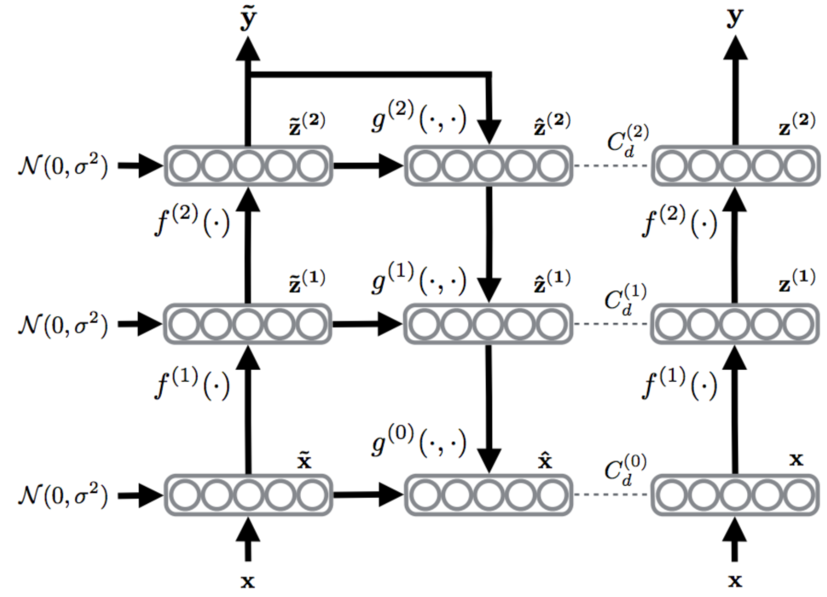
\includegraphics[width=\textwidth]{images/ladder_architecture}
  \caption{
    A conceptual illustration of a ladder network with two hidden layers ($L =
    2$). The feed-forward path ($\mathbf{x} \rightarrow \mathbf{z}^{(1)}
    \rightarrow \mathbf{z}^{(2)} \rightarrow \mathbf{y}$) shares the mappings
    $f^{(l)}$ with the corrupted feed-forward path, or encoder ($\mathbf{x}
    \rightarrow \mathbf{\tilde{z}}^{(1)} \rightarrow \mathbf{\tilde{z}}^{(2)}
    \rightarrow \mathbf{\tilde{y}}$). The decoder ($\mathbf{\hat{z}}^{(2)}
    \rightarrow \mathbf{\hat{z}}^{(1)} \rightarrow \mathbf{\hat{x}}$) consists
    of the denoising functions $g^{(l)}$ and has cost functions $C^{(l)}_{d}$
    on each layer aimed to minimize the difference between
    $\mathbf{\hat{z}}^{(l)}$ and $\mathbf{z}^{(l)}$. The output
    $\mathbf{\tilde{y}}$ of the encoder can also be trained to match available
    labels $t(n)$. Original figure found in the work of Rasmus et al.
    \cite{Rasmus:2015aa}.
  }
  \label{fig:ladder:architecture}
\end{figure}

Figure \ref{fig:ladder:architecture} shows the structure of a ladder network.
The corrupted path (left in the Figure) adds Gaussian noise $\mathcal{N}(0,
\sigma^{2})$ to each layer of the encoder. Every layer contributes to the cost
function, a term $C^{(l)} = ||\mathbf{z}^{(l)} - \mathbf{\hat{z}}^{(l)}||^{2}$
which trains the layers above (both encoder and decoder) to learn the denoising
function $\mathbf{\hat{z}}^{(l)} = g^{(l)}(\mathbf{\tilde{z}}^{(l)},
\mathbf{\hat{z}^{(l+1)}})$ which maps the corrupted $\mathbf{\tilde{z}}^{(l)}$
onto the denoised estimate $\mathbf{\hat{z}}^{(l)}$. As the estimate
$\mathbf{\hat{z}}^{(l)}$ incorporates all prior knowledge about $\mathbf{z}$,
the same cost function term also trains the encoder layers below to find
cleaner features which better match the prior expectation.

Since the cost function needs both the clean $\mathbf{z}^{(l)}$ and corrupted
$\mathbf{\tilde{z}}^{(l)}$, during training the encoder is run twice: a clean
pass for $\mathbf{z}^{(l)}$ and a corrupted pass for
$\mathbf{\tilde{z}}^{(l)}$. 

In denoising autoencoders \cite{Vincent:2010:SDA:1756006.1953039}, an
autoencoder is trained to reconstruct the original observation $\mathbf{x}$
from a corrupted version $\mathbf{\tilde{x}}$. Learning is based simply on
minimizing the norm of the difference of the original $\mathbf{x}$ and its
reconstruction $\mathbf{\hat{x}}$ from the corrupted $\mathbf{\tilde{x}}$; that
is the cost is $||\mathbf{\hat{x}} - \mathbf{x}||^{2}$. The main difference is
that in ladder networks the cost of reconstruction is calculated layer by layer
adding the denoising functions $\mathbf{\hat{z}} = g(\mathbf{z})$.

One way to picture the Ladder network is to consider it as a collection of
nested denoising autoencoders which share parts of the denoising machinery with
each other via the cost function $C_{d}$. If this function were not used, from
the viewpoint of the autoencoder on layer $l$, the representations on the
higher layers would be opaque, treated as hidden neurons. In other words, there
would be no particular reason why intermediate representation
$\mathbf{\hat{z}}^{(l+i)}$ as produced by the decoder should resemble the
corresponding representations $\mathbf{z}^{(l+i)}$ as produced by the encoder.
It is only the cost function $C^{(l+i)}_{d}$ that ties these together and
forces the inference to proceed in reverse order in the decoder. This sharing
helps a deep denoising autoencoder to learn the denoising process as it splits
the task into meaningful sub-tasks of denoising intermediate representations.

Batch normalization \cite{Ioffe:2015aa} is applied to each preactivation
including the topmost layer to improve convergence (due to reduced covariate
shift) and to prevent the denoising cost from encouraging the trivial solution
(encoder outputs constant values as these are the easiest to denoise). Direct
connection between a layer and its decoded reconstruction are used. The network
is called a Ladder network because the resulting encoder/decoder architecture
resembles a ladder because the cost function between mirroring layers could be
seen as the strings in ladder steps.

\subsubsection{Training of the network}

\begin{algorithm}[ht]
  \caption{Calculation of the output and cost function of the Ladder Network.
  Taken from Rasmus et al. \cite{Rasmus:2015aa}}
  \label{alg:ladder}
  \begin{multicols}{2}
  \begin{algorithmic}
    \REQUIRE $\mathbf{x}(n)$
    \STATE \# Corrupted encoder and training output
    \STATE {
      $\mathbf{\tilde{h}}^{(0)} \leftarrow \mathbf{\tilde{z}}^{(0)} \leftarrow
      \mathbf{x}(n) + \mathtt{noise}$
    }
    \FOR{ $l = 1$ \TO $L$ }
      \STATE {
        $\mathbf{\tilde{z}}^{(l)}_{\text{pre}} \leftarrow
        \mathbf{W}^{(l)}\mathbf{\tilde{h}}^{(l-1)}$
      }
      \STATE {
        $\boldsymbol{\tilde\mu}^{(l)} \leftarrow
        \mathtt{batchmean}(\mathbf{\tilde{z}}^{(l)}_{\text{pre}})$
      }
      \STATE {
        $\boldsymbol{\tilde\sigma}^{(l)} \leftarrow
        \mathtt{batchstd}(\mathbf{\tilde{z}}^{(l)}_{\text{pre}})$
      }
      \STATE {
        $\mathbf{\tilde{z}}^{(l)} \leftarrow
        \mathtt{batchnorm}(\mathbf{\tilde{z}}^{(l)}_{\text{pre}},
        \boldsymbol{\tilde\mu}^{(l)}, \boldsymbol{\tilde\sigma}^{(l)}) +
        \mathtt{noise}$
      }
      \STATE {
        $\mathbf{\tilde{h}}^{(l)} \leftarrow
        \mathtt{activation}(\boldsymbol{\gamma}^{(l)} \odot
        (\mathbf{\tilde{z}}^{(l)} + \boldsymbol{\beta}^{(l)}))$
      }
    \ENDFOR
    \STATE {
      $P(\mathbf{\tilde{y}} | \mathbf{x}) \leftarrow \mathbf{\tilde{h}}^{(L)}$ 
    }
    \STATE \# Clean encoder
    \STATE {
      $\mathbf{h}^{(0)} \leftarrow \mathbf{z}^{(0)} \leftarrow \mathbf{x}(n)$
    }
    \FOR{ $l = 1$ \TO $L$ }
      \STATE {
        $\mathbf{z}^{(l)}_{\text{pre}} \leftarrow
        \mathbf{W}^{(l)}\mathbf{h}^{(l-1)}$
      }
      \STATE {
        $\boldsymbol{\mu}^{(l)} \leftarrow
        \mathtt{batchmean}(\mathbf{z}^{(l)}_{\text{pre}})$
      }
      \STATE {
        $\boldsymbol{\sigma}^{(l)} \leftarrow
        \mathtt{batchstd}(\mathbf{z}^{(l)}_{\text{pre}})$
      }
      \STATE {
        $\mathbf{z}^{(l)} \leftarrow
        \mathtt{batchnorm}(\mathbf{z}^{(l)}_{\text{pre}},
        \boldsymbol{\mu}^{(l)}, \boldsymbol{\sigma}^{(l)})$
      }
      \STATE {
        $\mathbf{h}^{(l)} \leftarrow
        \mathtt{activation}(\boldsymbol{\gamma}^{(l)} \odot
        (\mathbf{z}^{(l)} + \boldsymbol{\beta}^{(l)}))$
      }
    \ENDFOR
    \STATE 
    \STATE \# Prediction output
    \STATE {
      $P(\mathbf{y} | \mathbf{x}) \leftarrow \mathbf{h}^{(L)}$ 
    }
    \STATE \# Decoder and denoising
    \FOR{ $l = L$ \TO $0$ }
      \IF { $l = L$ }
        \STATE { 
          $\mathbf{u}^{(L)}_{\text{pre}} \leftarrow \mathbf{\tilde{h}}^{(L)}$ 
        }
      \ELSE
        \STATE {
          $\mathbf{u}^{(l)}_{\text{pre}} \leftarrow
          \mathbf{V}^{(l+1)}\mathbf{\hat{z}}^{(l+1)}$ 
        }
      \ENDIF
      \STATE {
        $\boldsymbol{\mu}^{(l)} \leftarrow
        \mathtt{batchmean}(\mathbf{u}^{(l)}_{\text{pre}})$
      }
      \STATE {
        $\boldsymbol{\sigma}^{(l)} \leftarrow
        \mathtt{batchstd}(\mathbf{u}^{(l)}_{\text{pre}})$
      }
      \STATE {
        $\mathbf{u}^{(l)} \leftarrow
        \mathtt{batchnorm}(\mathbf{u}^{(l)}_{\text{pre}},
        \boldsymbol{\mu}^{(l)}, \boldsymbol{\sigma}^{(l)})$
      }
      \STATE {
        $\forall i : \hat{z}^{(l)}_{i} \leftarrow g(\tilde{z}^{(l)}_{i},
        u^{(l)}_{i})$
      }
      \STATE {
        $\forall i : \hat{z}^{(l)}_{i,\text{BN}} \leftarrow
        \frac{\hat{z}^{(l)}_{i} - \mu^{(l)}_{i}}{\sigma^{(l)}_{i}}$
      }
    \ENDFOR
    \STATE \# Cost function $C$ for training
    \STATE $C \leftarrow 0$
    \IF {t(n)}
      \STATE \# NLL cost for labeled data
      \STATE {
        $C \leftarrow -\log{P(\mathbf{\tilde{y}} = t(n) | \mathbf{x}(n))}$ 
      } 
    \ENDIF
    \STATE {
      $C \leftarrow C + \sum^{L}_{l=0} \lambda_{l} \left|\left|\mathbf{z}^{(l)}
      - \mathbf{\hat{z}}^{(l)}_{\text{BN}}\right|\right|^{2}$
    }
  \end{algorithmic}
  \end{multicols}
\end{algorithm}

Algorithm \ref{alg:ladder} lists the feed-forward pass of the full Ladder
network given one training instance (labeled or unlabeled). The results of the
algorithm are the prediction results $\mathbf{y}$ of the network as well as the
cost function $C$. As it can be seen from the figure, the algorithm goes
through the two paths of the encoder --clean and corrupted-- as well as the
decoder path. As seen in Algorithm \ref{alg:ladder} the cost function results
from the sum of the supervised cost given by the negative log-likelihood (if
applicable, i.e. the instance has a label), and the unsupervised cost of
reconstruction layer by layer. 

Algorithm \ref{alg:ladder}, however, shows how the cost function is obtained
for only one instance. For a batch of instances, the supervised cost function
is the average negative log probability of the noisy output
$\mathbf{\tilde{y}}$ matching the target $t(n)$ given the inputs
$\mathbf{x}(n)$

\[
  C_{c} = -\frac{1}{N} \sum^{N}_{n=1}\log{P(\mathbf{\tilde{y}} = t(n) |
  \mathbf{x}(n))}\text{.}
\]

The unsupervised denoising cost function, which is calculated layer by layer,
for more than one instance is

\[
  C_{d} = \sum^{L}_{l=0} \lambda_{l} C^{(l)}_{d} = \sum^{L}_{l=0}
    \frac{\lambda_{l}}{Nm_{l}} \sum^{N}_{n=1} \left|\left|\mathbf{z}^{(l)}(n) -
    \mathbf{\hat{z}}^{(l)}_{\text{BN}}(n)\right|\right|^{2} \text{,}
\]

where $m_{l}$ is the layer size, $N$ is the number of training instances, and
the hyperparameter $\lambda_{l}$ is a layerwise multiplier determining the
importance of the denoising cost. Finally, the cost function is obtained as the
sum of the supervised and unsupervised cost functions $C = C_{c} + C_{d}$.

Both in the encoders --clean or corrupted-- and the decoder, each layer uses
batch normalization, as explained before, to improve convergence and prevent
the denoising cost from encouraging the trivial solution. The clean path
differs from the corrupted path in that the latter adds gaussian noise before
activation. Also, the corrupted output is used for training but the clean
output is used for prediction.

The function $g$ is the {\em combinator function} such that
$\text{\textbf{z}}^{(l)} = g(\tilde{\text{\textbf{z}}}^{(l)},
\hat{\text{\textbf{z}}}^{(l+1)})$ which can approximate the optimal denoising
function for the family of observed distributions. The function $g$ is
therefore expected to form a reconstruction $\hat{\text{\textbf{z}}}^{(l)}$
that resembles the clean $\text{\textbf{z}}^{(l)}$ given the corrupted
$\tilde{\text{\textbf{z}}}^{(l)}$ and the higher-level reconstruction
$\hat{\text{\textbf{z}}}^{(l+1)}$.

The work by Rasmus et al. \cite{Rasmus:2015aa} presents the instatiation of
$g$ that I used in the implementation for the experiments of this chapter.
However, there can be other versions of the combinator function. Pezeshki et
al. \cite{Pezeshki:2015aa} presented another version of the combinator function
which, they claim, outperforms the original. Further experimentation with other
combination functions, or even the design of a combinator function for the task
of Spanish \vsd~in particular, is left for future work. The combinator function
used for this experiments, defined by Rasmus et al. \cite{Rasmus:2015aa}, is
the following:

\[
  \hat{z}^{(l)}_{i} = g_{i}(\tilde{z}^{(l)}_{i}, u^{(l)}_{i}) =
    \left(\tilde{z}^{(l)}_{i} -
    \phi_{i}(u^{(l)}_{i})\right)\psi_{i}(u^{(l)}_{i}) + \phi_{i}(u^{(l)}_{i})
    \text{,}
\]

Where the functions $\phi_{i}(u^{(l)}_{i})$ and $\psi_{i}(u^{(l)}_{i})$ are
modeled as expressive nonlinearities:

\begin{align*}
  \phi_{i}(u^{(l)}_{i}) &= a^{(l)}_{1,i}\sigma(a^{(l)}_{2,i}u^{(l)}_{i} +
    a^{(l)}_{3,i}) + a^{(l)}_{4,i}u^{(l)}_{i} + a^{(l)}_{5,i} \\
  \psi_{i}(u^{(l)}_{i}) &= a^{(l)}_{6,i}\sigma(a^{(l)}_{7,i}u^{(l)}_{i} +
    a^{(l)}_{8,i}) + a^{(l)}_{9,i}u^{(l)}_{i} + a^{(l)}_{10,i}
  \text{,}
\end{align*}

where $\sigma$ is the {\em sigmoid function}.

The model has the following trainable parameters, which can be trained simply
by using the back-propagation algorithm to optimize the cost function $C$:

\begin{description}
  \item[$\mathbf{W}^{(l)}$, $\mathbf{V}^{(l)}$] The weight matrices of the
    encoder and decoder respectively for each layer $l$ of the network. Note
    that $\mathbf{V}^{(l)}$ has the same dimension as the transpose of
    $\mathbf{W}^{(l)}$.
  \item[$\boldsymbol{\gamma}^{(l)}$, $\boldsymbol{\beta}^{(l)}$] The bias and
    scaling parameters respectively for each layer $l$ of the network.
  \item[$a^{(l)}_{1,i},\dots,a^{(l)}_{10,i}$] The parameters of the functions
    $\phi_{i}(u^{(l)}_{i})$ and $\psi_{i}(u^{(l)}_{i})$, proposed by the
    authors.
\end{description}

The cost function $C$ is minimized using stochastic gradient descent. On each
iteration (also called epoch), the algorithm takes a batch of elements of the
same size both from the labeled and the unlabeled dataset. It uses those
elements to do a forward propagation. This goes on batch by batch until all the
instances in one of the two datasets, either the labeled or unlabeled dataset,
have been used for training. Normally, the labeled dataset is smaller than the
unlabeled dataset, so it usually happens that the labeled dataset is consumed
much sooner than the unlabeled dataset. Then, the dataset that has been
completely used for training (usually the supervised dataset) is shuffled and
the algorithm starts over to take batches from that dataset as if it were new.
The dataset that has not been fully used up keeps being consumed in the same
way. Using the original implementation of the algorithm, the size of the batch
was equal to the size of the labeled dataset. This means that on each iteration
the ladder network minimized the cost function over the whole labeled data
(with a random order) and a chunk of the unlabeled dataset (which is larger).

\subsubsection{Hyperparameters}

The ladder network algorithm has an important number of hyperparameters to tune
and experiment with. Some of these hyperparameters are given by the neural
network (e.g. the number and size of the layers), others are given by the
ladder network model (e.g. the scaling factor for noise) and others are given
by the training procedure (e.g. the stopping criterion). As the number of
experiment grows exponentially the more hyperparameters I tune, I decided to
keep it as simple as possible to avoid losing focus of the experimentation of
the chapter.

First of all is the structure of the network. To keep a comparison point with
the experiments of previous chapters, the encoder has three hidden layers ($L =
3$) with 500, 250 and 100 neurons each. As such, the decoder, which is
symmetric to the encoder, has three layers with 100, 250 and 500 neurons each.

The hyperparameters defined by the ladder network algorithm are the scaling
factor for noise in the corrupted encoder, and the layer-wise factor that
denotes the imporance of each denoising cost (i.e. $\lambda_{l}$). To avoid an
exponential growth in the number of experiments I decided to use the
hyperparameters described in the experiments in the work by Rasmus et al. The
scaling factor for noise was $0.3$ and the importance of the denoising cost
layers was set to $\lambda^{(0)} = 1000$, $\lambda^{(1)} = 10$, and
$\lambda^{(l \geq 2)} = 0.01$.

\subsubsection{Stopping criterion}

Ladder networks, unlike the wrapper algorithms I discussed before, do not start
from a supervised algorithm that was previously trained on the supervised data.
Instead it learns by minimizing the objective function with both supervised and
unsupervised data from scratch. Thus, the way to stop the algorithm is
precisely by looking for convergence or by establishing a maximum number of
iterations.

I added another stopping criterion to avoid the ladder networks algorithm to
overfit the supervised dataset. Section \ref{sec:self-learning:algorithm}
explains that for self-learning 20\% of the training data is reserved for
validation, ensuring that each class is represented at least by one example in
both corpora. I use this same technique to select a validation dataset from the
training data. The validation dataset serves to check at every iteration that
the algorithm is not reducing the cost error at the expense of generalization.

The stopping criterion then became one of three:

\begin{enumerate}
  \item The algorithm reached the maximum number of given iterations.
  \item The error in the cost function converges: the error of a new iteration
    is larger than or equal to the error of the previous iteration plus some
    error tolerance $\epsilon$.
  \item The validation dataset error is larger than or equal to the previous
    validation error registered by the algorithm plus some error tolerance
    $\eta$.
\end{enumerate}

A set of experiments was done to verify which values of $\eta$ and $\epsilon$
improve the convergence of the model without losing too much information.
However, in the experiments, the value that really made a difference was the
number of iterations as I will discuss further in the chapter.

\subsection{Experiments}

The experiments presented in this section help in the acceptance or rejection
of the presented hypotheses in the beginning of this chapter.

First, Hypothesis \ref{hyp:ladder:1} calls for an experiment to compare between
ladder networks and the algorithms seen so far: supervised, self-learning and
active learning. Experiment \ref{exp:ladder:1} tests the ladder network model
on the held-out test set and uses that to compare it to the previous
algorithms.

\begin{experiment}\label{exp:ladder:1}
  \begin{enumexp}
    \item Train the model with ladder networks until a stopping criterion is
      met.
    \item Evaluate the model on the held-out test dataset.
  \end{enumexp}
\end{experiment}

Experiment \ref{exp:ladder:2} reports the distribution of classes taking into
account both the labeled data and some automatically annotated data taken from
an unlabeled pool of examples different from the one given to the ladder
network to minimize the unsupervised cost function.

\begin{experiment}\label{exp:ladder:2}
  \begin{enumerate}
    \item Run the ladder network algorithm over the labeled dataset $L_{1}$ and
      the unlabeled dataset $U_{1}$.
    \item In each iteration use the model obtained so far to predict the labels
      of a pool of unlabeled data $U_{2}$, different from the data in unlabeled
      dataset $U_{1}$.
    \item From that pool annotate those with a predicted class which the model
      has a certainty over a threshold. This threshold is calculated following
      the steps described on Section \ref{sec:self-learning:algorithm}: it
      starts at 100\% and it is slowly lowered until it has at most a certainty
      that is 10\% more than the random chance. 
    \item Take those automatically annotated instances off the unlabeled pool.
      If there is no instance on which the model has the required certainty, do
      not annotate any instance.
    \item Record the distribution of the classes of both the labeled dataset
      and the automatically labeled instances obtained so far.
  \end{enumerate}
\end{experiment}

Experiment \ref{exp:ladder:3} measures the tendency to overfit of the ladder
network classifier. It does so by monitoring both the training dataset and the
validation dataset. This is very similar to what self-learning does. However,
in this case the number of examples in the model is not augmented since the
model itself does not add unannotated examples. However, recall that each
training iteration takes the whole supervised dataset and only a portion of the
unsupervised dataset. Thus on each iteration the algorithm adds more
information from the unsupervised data by aiming to minimize the unsupervised
part of the cost function of the algorithm. This is until the algorithm has
covered all the unlabeled instances. After that, the algorithm does not add new
data to the model, but carries on successive iterations aimed to fit better the
available data. Nevertheless, to compare with the previous algorithms, for this
experiment the algorithm stops after it traverses the whole unlabeled dataset
once.

\begin{experiment}\label{exp:ladder:3}
  \begin{enumexp}
    \item Take only a portion of the whole unsupervised dataset to use as
      unsupervised data for the algorithm.
    \item Shuffle both training and validation datasets and split them randomly
      with stratified sampling.
    \item Start the ladder networks algorithm.
    \item In each step, run an iteration of training and record the predictions
      over training and validation data.
    \item Stop the algorithm once the whole unlabeled dataset is traversed
      once.
    \item Repeat the whole procedure {\em n} times with a different portion of
      the unsupervised dataset, until the whole unsupervised dataset is
      traversed.
  \end{enumexp}
\end{experiment}

\subsection{Metrics}

The results of Experiment \ref{exp:ladder:1} are reported with the F1-score for
each class in the test dataset of the token lemmas. This is done for each of
the four algorithms seen so far: supervised, self-learning, active learning and
ladder networks.

The results of Experiment \ref{exp:ladder:2} report the proportional count of
elements of each class as done for the experiments in previous chapters of this
thesis.

Finally, for Experiment \ref{exp:ladder:3} I use the error due to variance
defined by Metric \ref{met:3} to report the results of the experiment. This
measures the model tendency to overfit as new unlabeled data is added to the
model.

\section{Analysis of results}\label{sec:ladder:results}

This section reports the results obtained by the experiments and measures by
the metrics I explained previously.

In a first set of experiments, I run the algorithm for a total of 100
iterations. However, the algorithm did not stop because it converged, but rather
because of reaching the maximum number of iterations. Nevertheless, by the
100th iteration the improvement on the error was low enough to consider the
algorithm had converged.

Nevertheless, as I will show next, once I visualized the results regarding the
distribution of classes (Experiment \ref{exp:ladder:2}), I found that when the
algorithm was about 25 iterations the distribution of the classes began to
drift to the most frequent one (regardless of the lemma). Thus I decided to run
the same experiments with 25 iterations only and see what the results were. 

Of course these results are just a view of the data available that I will try
to interpret as objectively as possible. However, there might be some results
that are obscured by the chosen visualizations.

\subsection{Hypothesis \ref{hyp:ladder:1}}\label{sec:ladder:hyp:1}

Hypothesis \ref{hyp:ladder:1} states that the ladder network model improves
over the purely supervised and other semi-supervised methods on a held-out test
corpus. To test this Hypothesis I measure the results of Experiment
\ref{exp:ladder:1} which asseses the impact of using a ladder network model in
the task of Spanish \vsd. These results are compared with the performance
results of the previous algorithms in the test corpus. The metric to report the
results is the F1-score per class. As I explained before, I will show the
results training the ladder network with 100 iterations and also with 25
iterations.

As this is only done in the held-out test dataset, the performance showed in
this Section is done for the most frequent, second most frequent and, if it
applies, third most frequent class of the lemma. Recall that only two of the
six lemmas had three classes in the held-out test dataset: ``llegar'' and
``pensar''. The other four lemmas had only two classes in the dataset.

\begin{figure}[hb!]
  \centering
  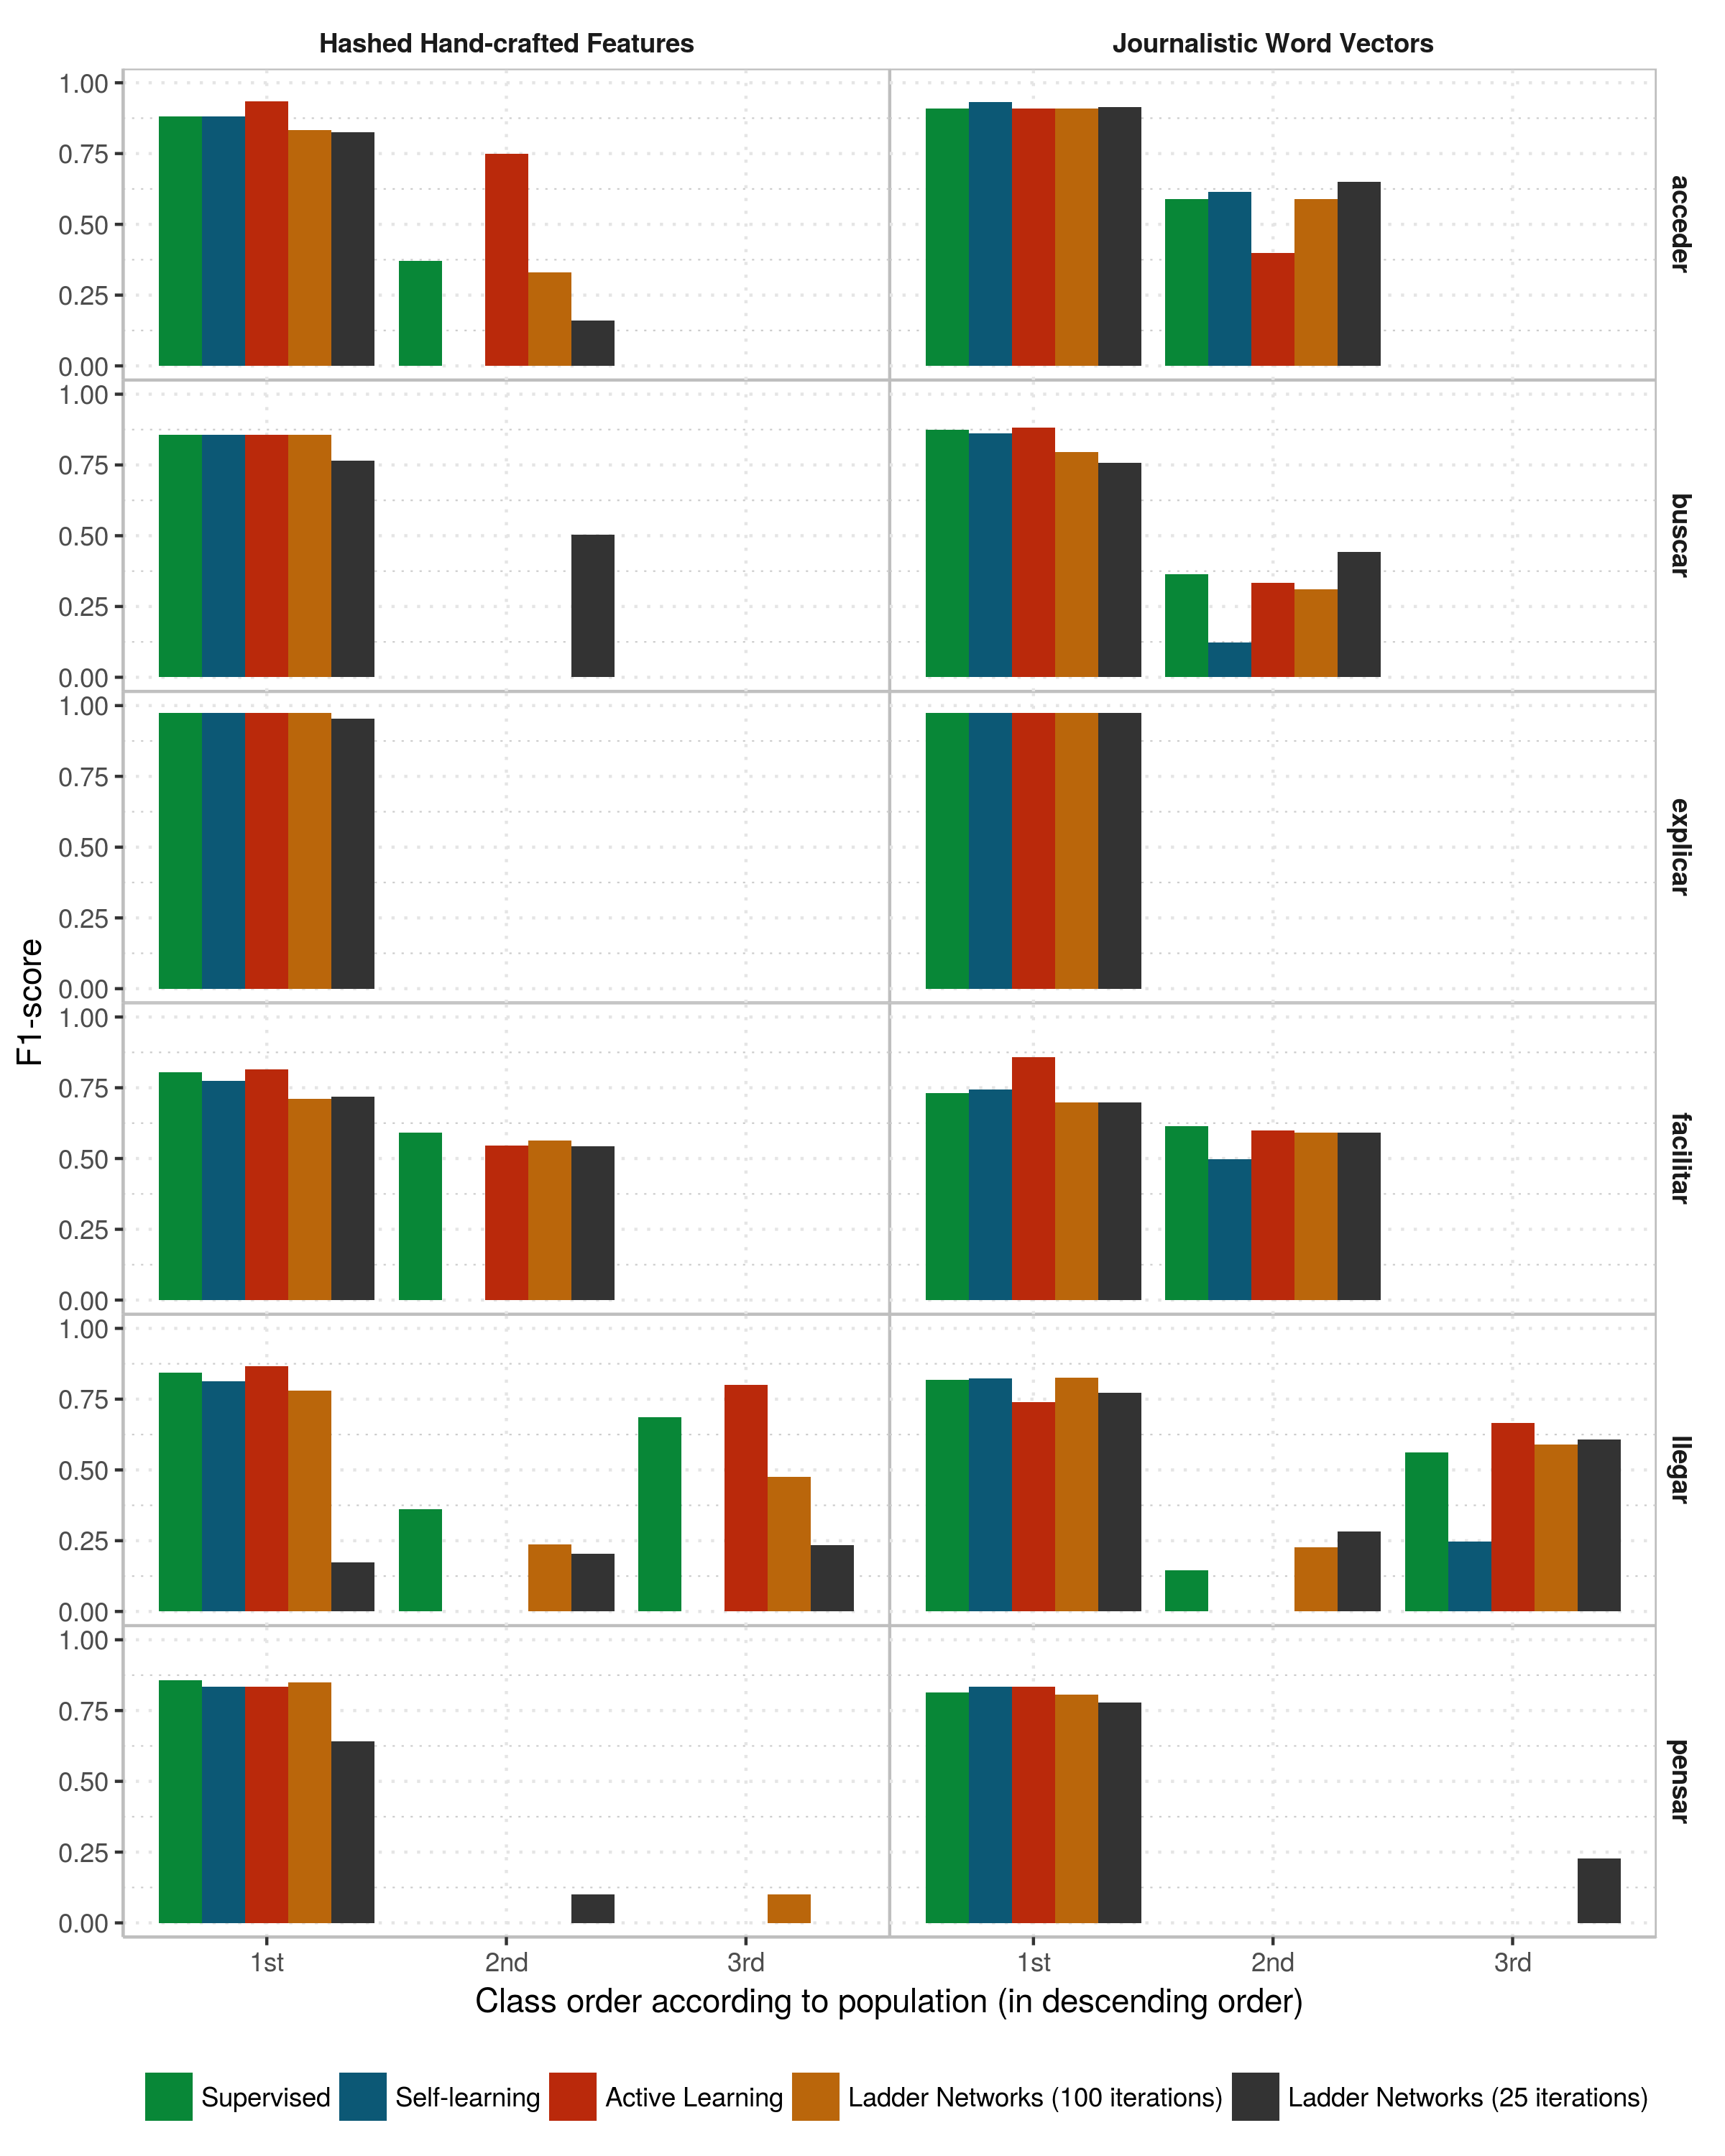
\includegraphics[height=0.9\textheight,width=\textwidth,keepaspectratio]
    {plots/ladder/per_sense_fscore}
  \caption{Comparison of macro and weighted average F1-score for supervised,
  self-learning, active learning, and ladder networks (using 100 iterations
  first and using 25 iterations secondly)}
  \label{fig:ladder:performance}
\end{figure}

Figure \ref{fig:ladder:performance} shows the F1-score macro and weighted
average for supervised, self-learning, active learning, and ladder networks
(using 100 iterations) over the test dataset. In this case, ``supervised'' is
the evaluation of the model in the initial iteration of any of the wrapper
algorithms (as it is the same for both, i.e. only using the manually labeled
data). The self-learning/active learning/ladder networks bars represent the
performance of the model over the held-out test dataset after finishing the
iterations of the corresponding algorithm. The structure of the graphic is as
follows:

\begin{itemize}
  \item Each row shows the results for a token lemma: ``acceder'', ``buscar'',
    ``explicar'', ``facilitar'', ``llegar'', and ``pensar''.
  \item Each column stands for a feature representation: hand-crafted hashed
    features and journalistic word vectors.
  \item Each group of bars in each plot represents the class (i.e. sense) for
    that lemma. These are ordered according to number of occurrences of the
    class in the dataset.
  \item Each bar plot in a different color inside a group represents the
    algorithm: supervised (i.e. evaluation moment of the initial iteration for
    a wrapper algorithm, in this case self-learning), self-learning (i.e.
    evaluation moment of the final iteration after self-learning finishes),
    active learning (i.e. evaluation moment of the final iteration after active
    learning finishes), and two versions of ladder networks (i.e.
    distinguishing different moments when the ladder networks algorithm stops,
    in this case after reaching 100 or 25 iterations).
  \item The height of the bar represents the value of the F1-score per each
    class.
\end{itemize}

Once again, recall that only the last two rows of the graphic represent the
lemmas with 3 senses (i.e. ``llegar'' and ``pensar''). The first four lemmas
can at most show results for two senses.

Note that ladder networks (in either case) performs equally or even better than
active learning in most of the senses. Remember that so far active learning
have shown the best results as it can be appreciatted in the Figure.

Moreover, there are a couple of cases where the ladder network (with 100 or 25
iterations) performs better than supervised learning on a class that supervised
learning does not recognize at all (e.g. the third most frequent class of the
lemma ``pensar''). Of course this might happen by random chance, but it is
still something to consider as ladder networks, unlike active learning, is
completely automatic (i.e. there is no human involvement). Moreover it happens
differently for ladder networks using 100 iterations and using 25 iterations.

Clearly, ladder networks is also a better alternative (or at least has better
performance) than self-learning. And it also has better performance using word
embeddings than using hand-crafted features, as we have seen along this thesis.

Notice also that in general (specially for word embeddings) stopping ladder
networks at 25 iterations has better performance than going the full 100
iterations. As I will show further, around 25 iterations begins the drift to
the most frequent class which is a good indication that this is why ladder
networks with only 25 iterations performs better than with 100 iterations.
Notice specially that ladder networks with 25 iterations tend to perform worse
than ladder networks with 100 iterations for the case of the most frequent
class. This is yet more evidence that stopping the algorithm when it begins to
drift to the most frequent class is a good solution to the problem of having
worse performance for less frequent classes.

In summary, ladder networks present some impressive results, specially in
comparison to active learning and taking into account that it is a purely
automatic method. It has much better results also than self-learning and it
seems that more insightful diagnostics over the iterations of the algorithm can
help balance the performance for the classifier on classes besides the most
frequent one. 

Even if ladder networks are not the best solution for all the cases, it is
clear that being a semi-supervised method that is completely automatic, it
improves on what other methods can achieve. E.g. the model has more
information, and thus more coverage, than a purely supervised method, and it
also avoids the use of an oracle for the annotation procedure. From these
results I accept Hypothesis \ref{hyp:ladder:1} that ladder networks improves
over the purely supervised or other semi-supervised methods. It can be argued
that, even if the raw performance of the purely supervised approach and the
active learning approach is comparable to that of ladder networks, the latter
are less expensive than active learning and in general do a better job of
maintaining good performance in all classes.

\subsection{Hypothesis \ref{hyp:ladder:2}}\label{sec:ladder:hyp:2}

Hypothesis \ref{hyp:ladder:2} was planned to compare how ladder networks work
when facing a similar task to that of the wrapper algorithms I explored in the
previous chapters. The hypothesis states that the representativity of the
classes if using the model to classify some unsupervised data will be
maintained through the iterations. In particular, it was in the visualization
of this experiment's results that I found that around iteration number 25 there
was a drifting of the algorithm to the most frequent class. In this section
there are two plots of the same results, varying only in the number of
iterations the ladder network algorithm is given to finish.

Like for self-learning and active learning in the previous chapter, to analyze
these results I use two forms of visualization: one explores the distribution
of the classes along the iterations of the algorithm and the other explores the
proportional count of each class added on each iteration of the algorithm.

\subsubsection{Classes' population distribution across iterations}

\begin{figure}[htb!]
  \centering
  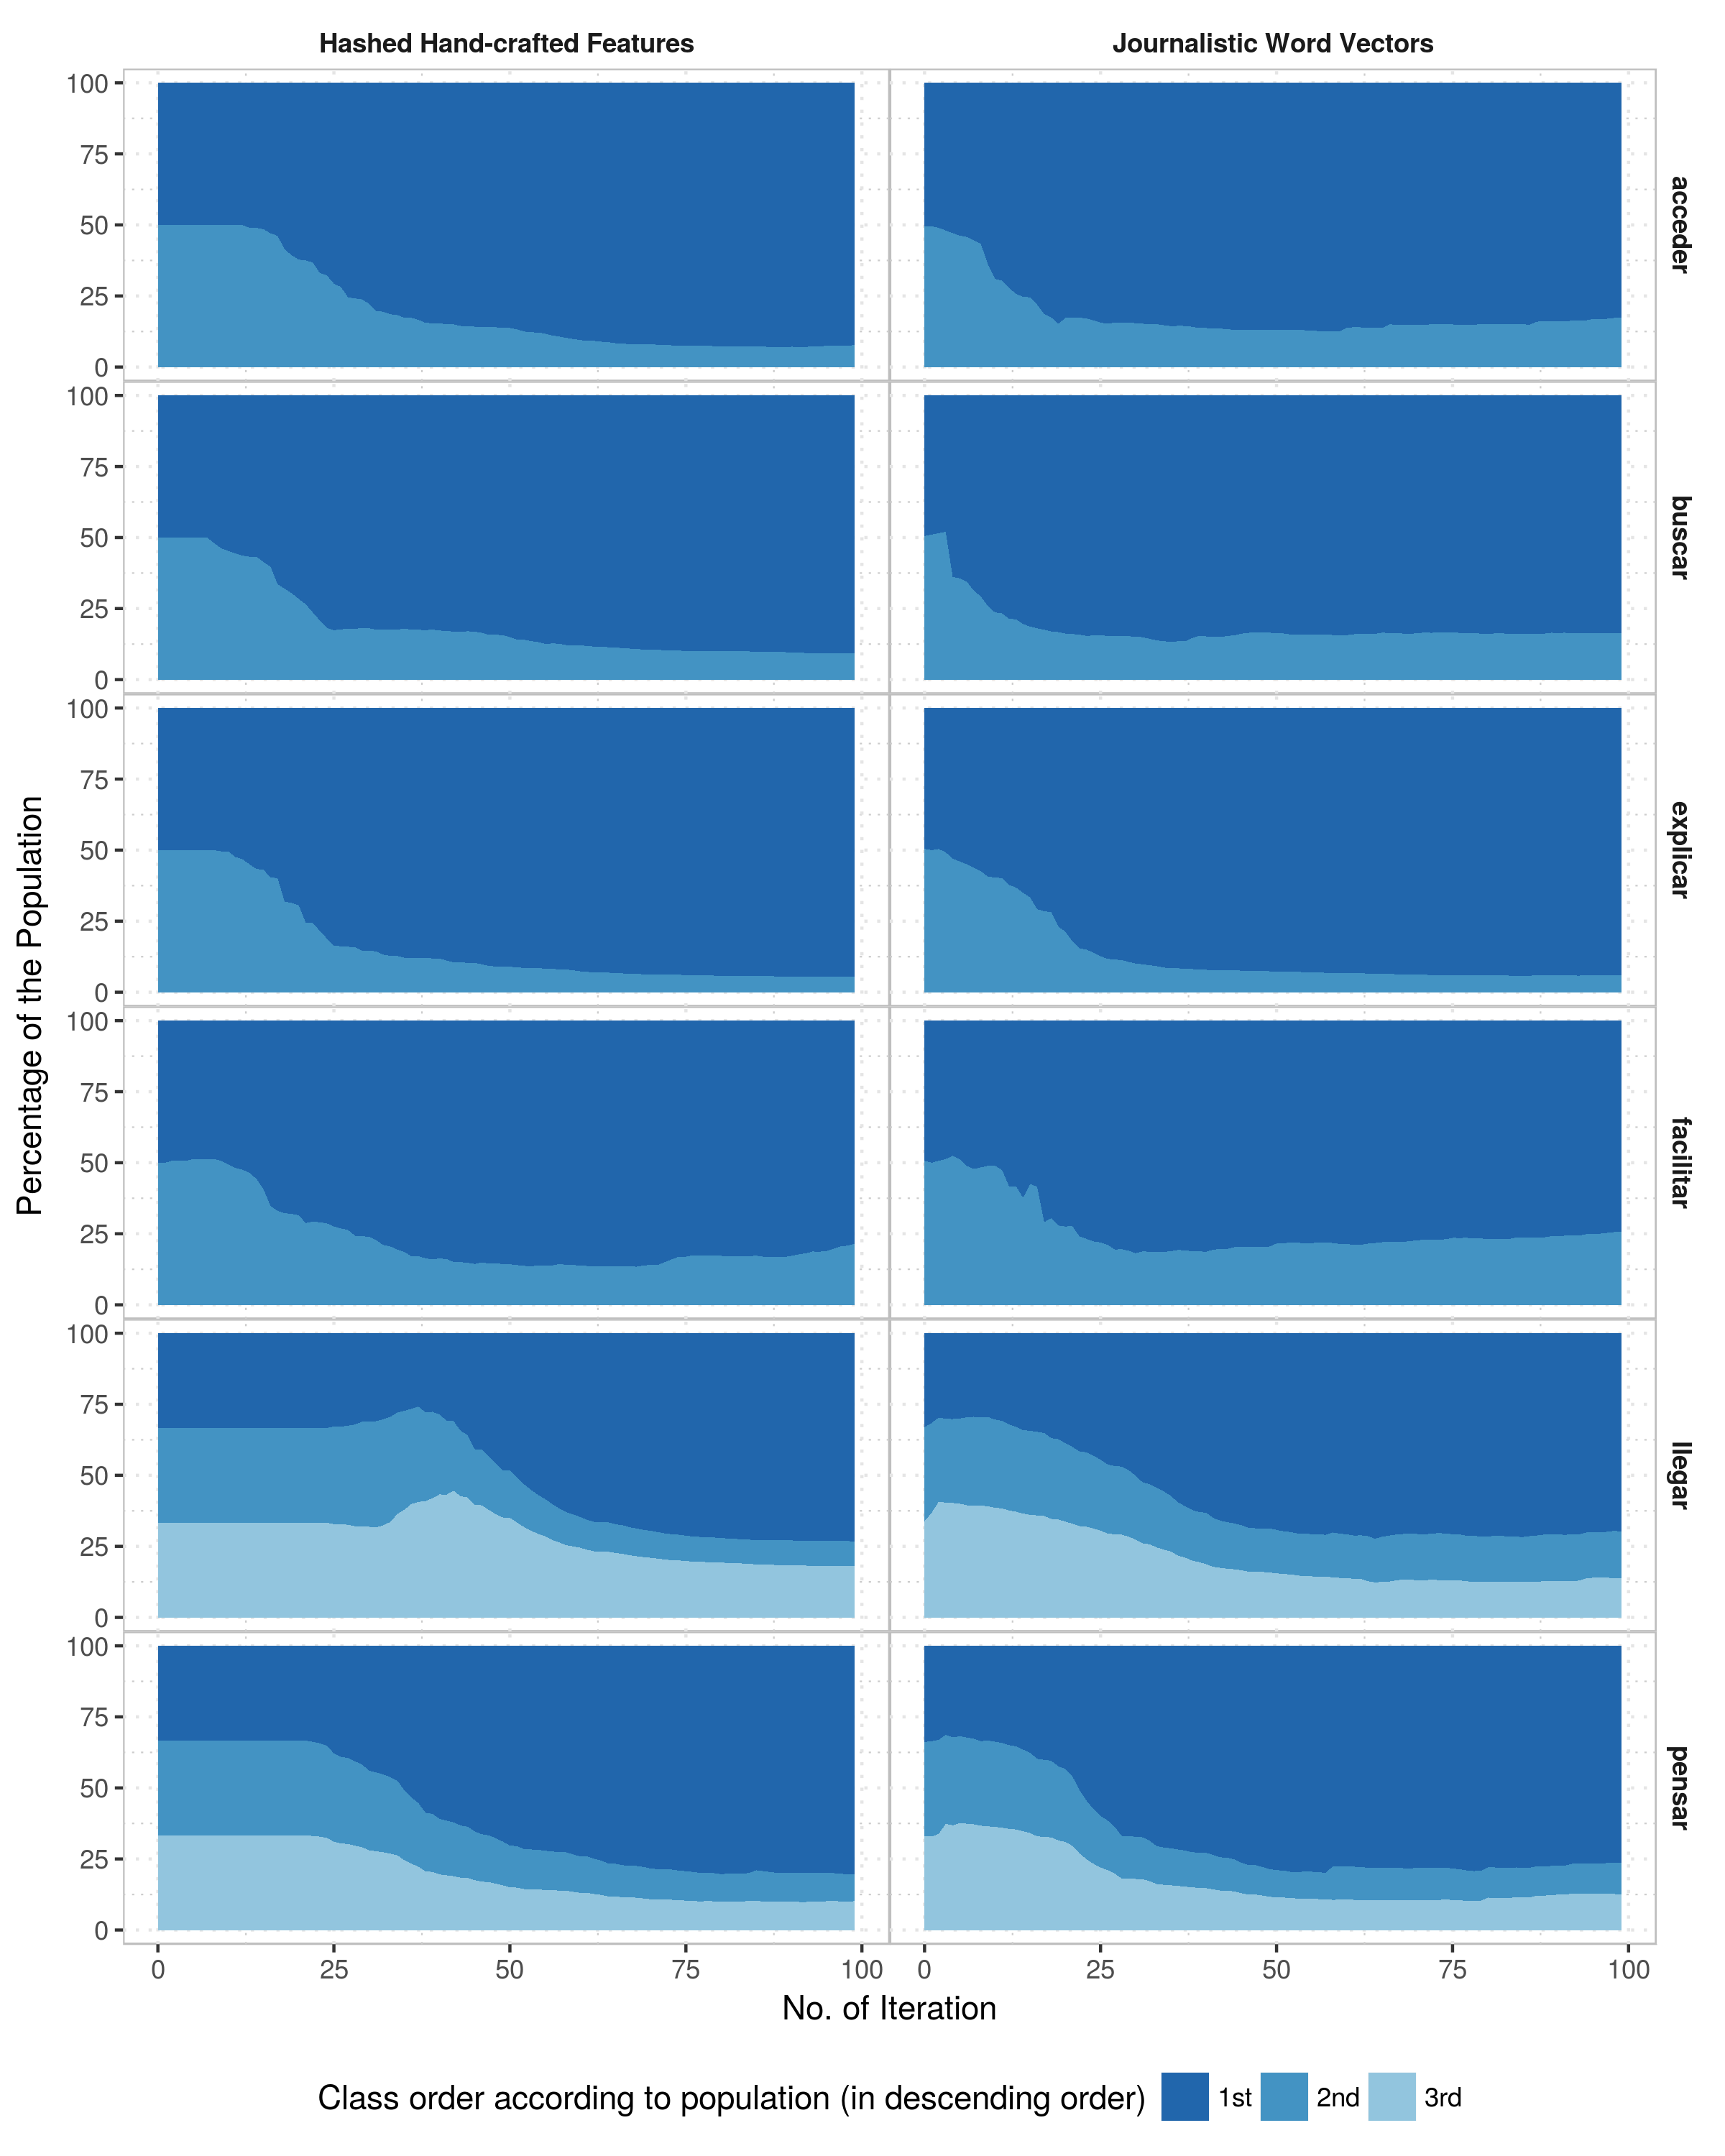
\includegraphics[height=0.9\textheight,width=\textwidth,keepaspectratio]
    {plots/ladder/population_distribution_100}
  \caption{Distribution of the classes' population across ladder networks
  algorithm's iterations (with a maximum of 100 iterations) as a proportion of
  the whole training dataset}
  \label{fig:ladder:population_distribution:100}
\end{figure}

\begin{figure}[hb!]
  \centering
  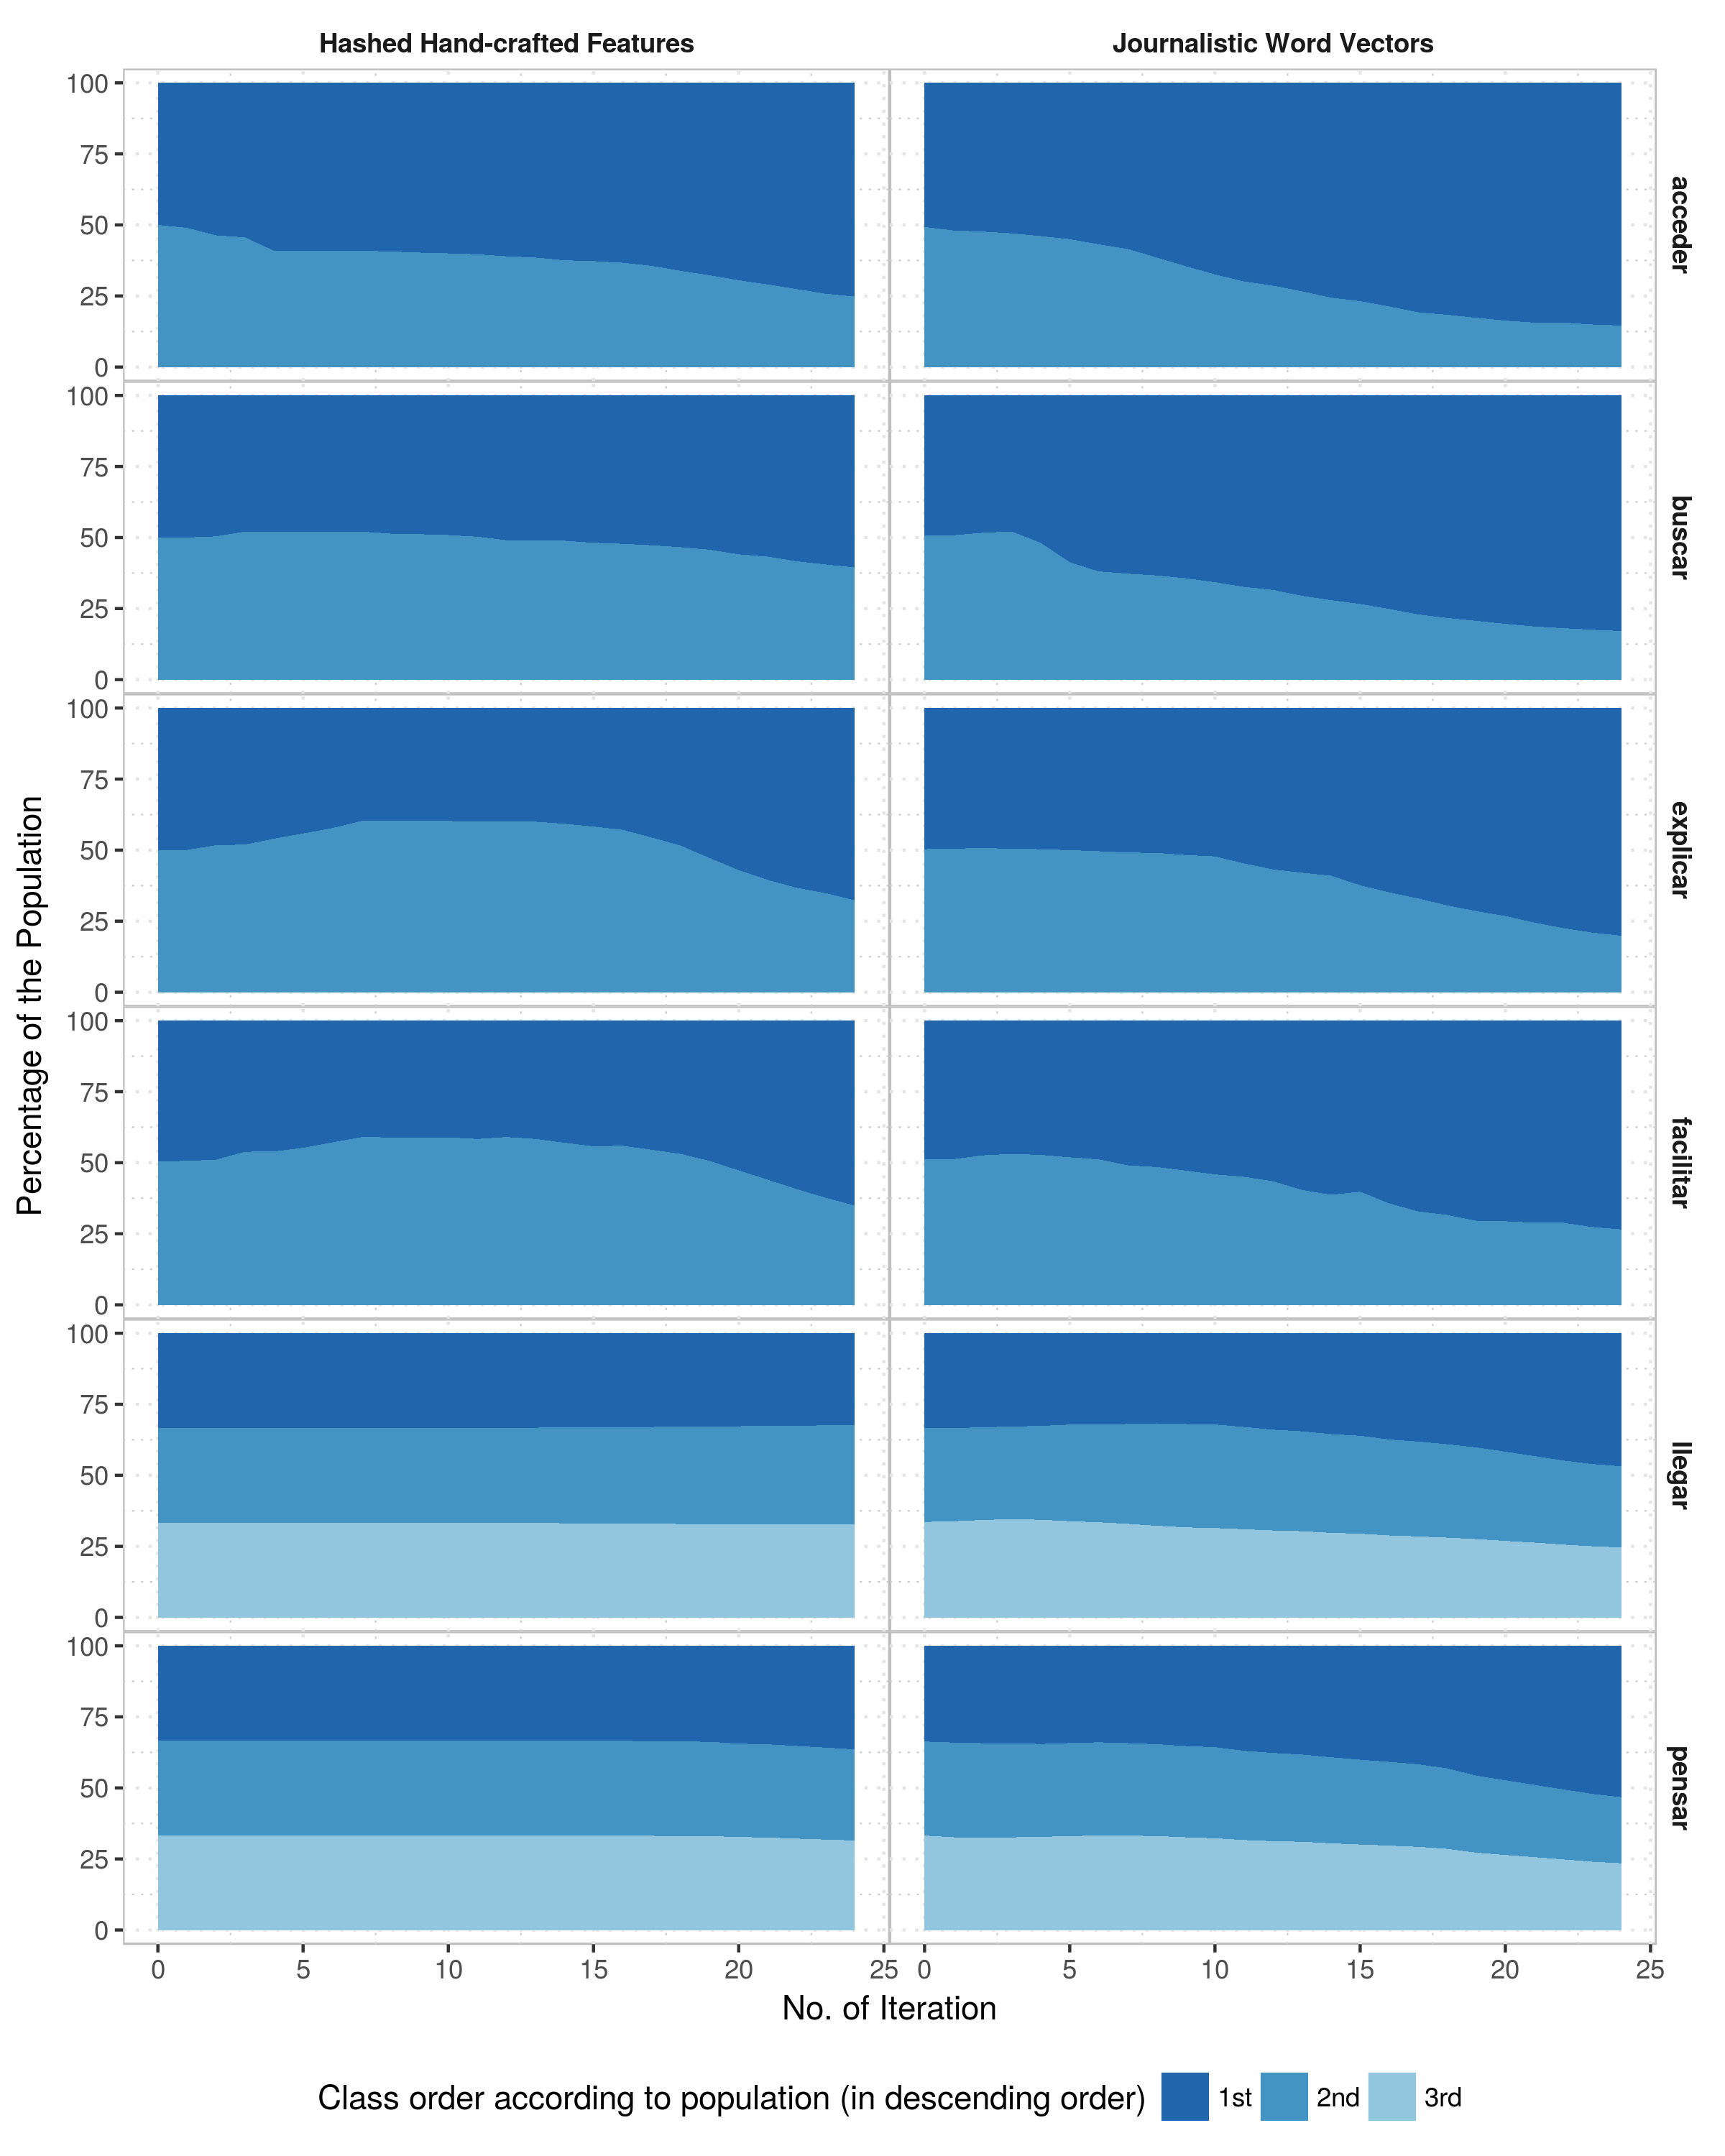
\includegraphics[height=0.9\textheight,width=\textwidth,keepaspectratio]
    {plots/ladder/population_distribution_25}
  \caption{Distribution of the classes' population across ladder networks
  algorithm's iterations (with a maximum of 25 iterations) as a proportion of
  the whole training dataset}
  \label{fig:ladder:population_distribution:25}
\end{figure}

Figure \ref{fig:ladder:population_distribution:100} shows the distribution of
the population of the classes across ladder network iterations (with a maximum
of 100 iterations) of the algorithm. Each class's population is represented as
the proportion of the total number of examples in the training dataset for that
iteration. The plot is a stacked area plot that follows this structure:

\begin{itemize}
  \item Each row shows the results for a token lemma: ``acceder'', ``buscar'',
    ``explicar'', ``facilitar'', ``llegar'', and ``pensar''.
  \item Each column stands for a feature representation: hand-crafted hashed
    features and journalistic word vectors.
  \item The x-coordinate represents the iteration in the self-learning
    algorithm.
  \item The y-coordinate represents the percentage of population.
  \item Each area of a different color represents the proportion of examples
    for each of the classes in the dataset. The classes again are ordered
    according to number of examples in the original supervised dataset.
\end{itemize}

As I already explained in previous sections of this chapter, it is around the
iterations number 25 (although not in all cases, in some cases is much earlier
and in some is later) that the distribution of the classes from the labeled and
automatic annotated classes of the unlabeled corpus used for the task (as
described in Experiment \ref{exp:ladder:3}) begin to drift to the most frequent
class. Once again, the prevalence of the most frequent class is more acute for
hand-crafted features than for journalistic word embeddings.

If I decide to stop the algorithm by the iteration number 25, the distribution
of classes looks like the one in Figure
\ref{fig:ladder:population_distribution:25}. The figure has the exact same
structure as the previous figure with the only difference being in the maximum
number of training iterations of the ladder network model.

In this case however, the drift of the model to automatically annotate
everything as the most frequent class is not so strong as in the previous
figure. The algorithm stops before that happens (although there are exceptions,
after all, like all, each lemma has its own set of properties the algorithm
needs to adapt to).

In any case, the drifting of the ladder network model to the most frequent
class is not as strong as in self-learning, where it is practically immediate,
right after the first iteration. This can well be a consequence of the ladder
network learning the model through the iterations as it slowly gains confidence
of the decision boundaries. Unlike in self learning, the use of unlabeled data
in this case serves to delay and avoid the drift to the most frequent class.

Eventually, with more iterations, the most frequent class starts gaining more
and more probability, which is expected as the data has a Zipfian distribution.
However, the fact that the results on the test dataset are better than those
for self-learning seems to indicate that the ladder network is actually
classifying the examples of the most frequent class correctly (better
precision), unlike self-learning, which might well classify them as majority
class just because it cannot tell them apart from any other class.

\subsubsection{Population added per sense per iteration}

\begin{figure}[hb!]
  \centering
  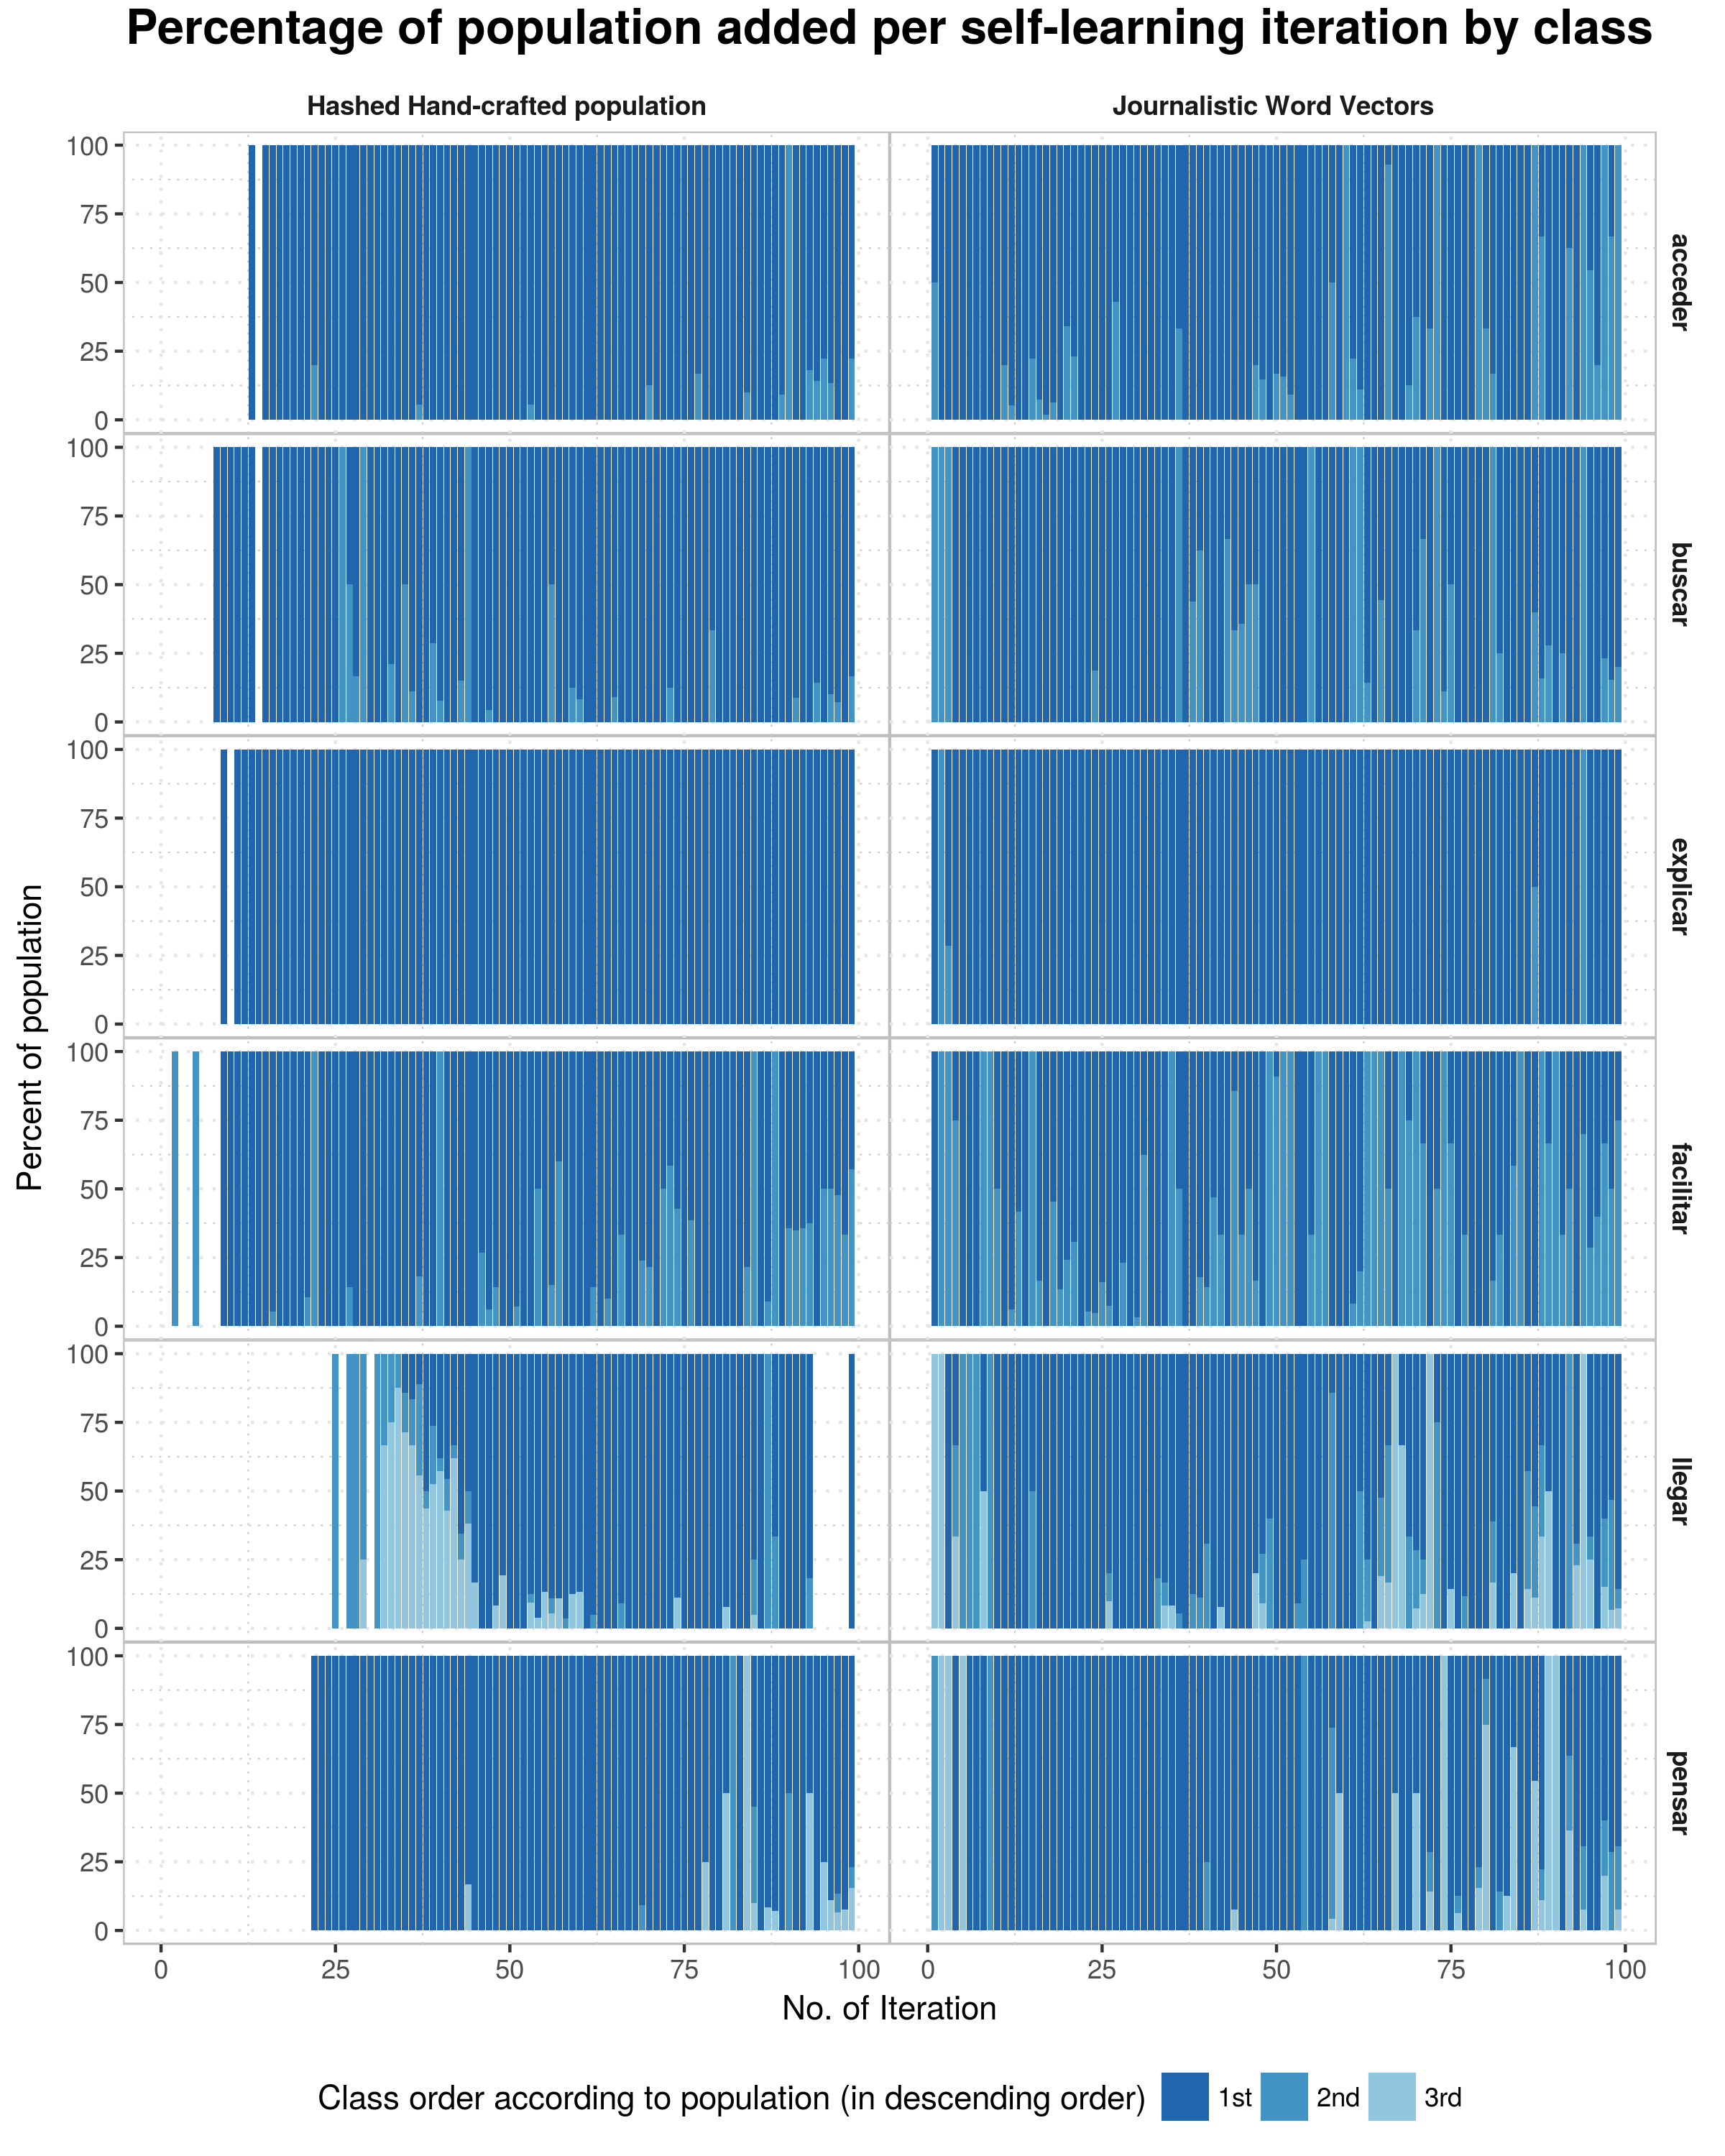
\includegraphics[height=0.9\textheight,width=\textwidth,keepaspectratio]
    {plots/ladder/population_add_per_class_100}
  \caption{Population added per sense on each iteration of ladder network (with
  a maximum of 100 iterations) as a proportional count of all the examples
  added in that iteration}
  \label{fig:ladder:population_add_per_class:100}
\end{figure}

\begin{figure}[htb!]
  \centering
  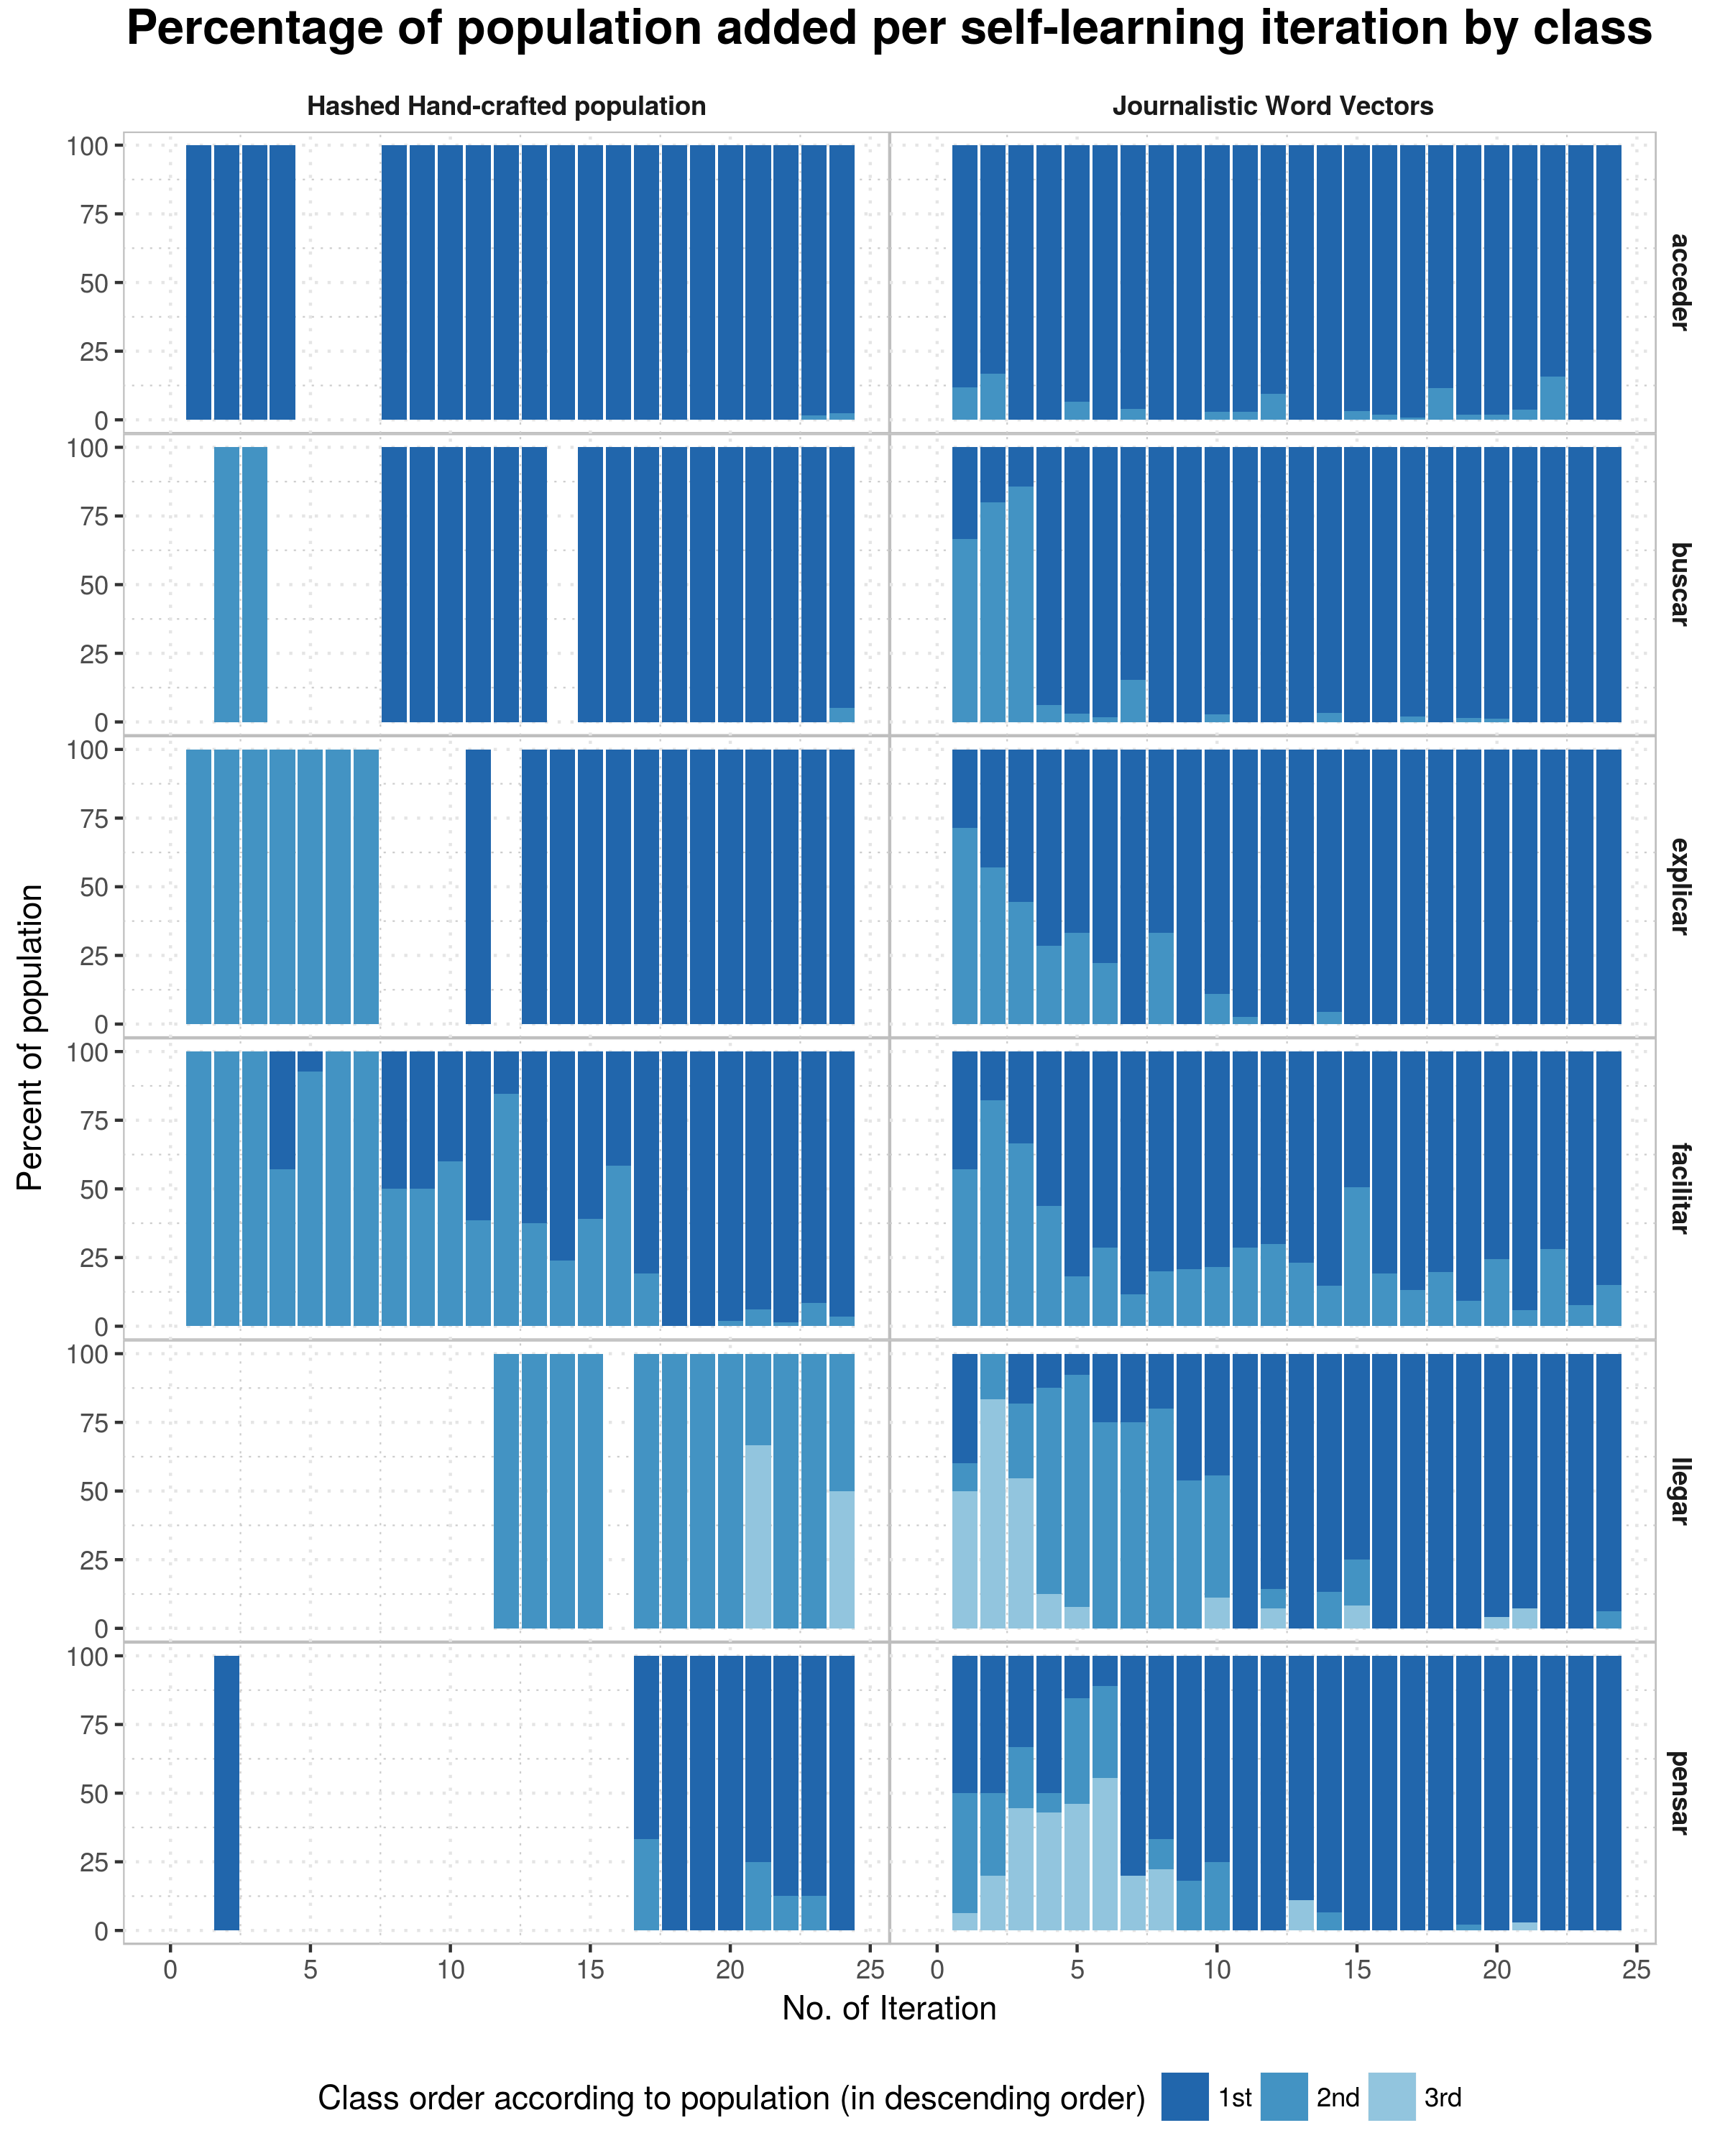
\includegraphics[height=0.9\textheight,width=\textwidth,keepaspectratio]
    {plots/ladder/population_add_per_class_25}
  \caption{Population added per sense on each iteration of ladder network (with
  a maximum of 25 iterations) as a proportional count of all the examples
  added in that iteration}
  \label{fig:ladder:population_add_per_class:25}
\end{figure}

Figure \ref{fig:ladder:population_add_per_class:100} shows the proportion of
examples added per class on each iteration. It is a stacked bar plot where each
bar represents the total examples added in the iteration split by the
proportion of classes automatically annotated as such. The structure of the
plot is the following:

\begin{itemize}
  \item Each row shows the results for a token lemma: ``acceder'', ``buscar'',
    ``explicar'', ``facilitar'', ``llegar'', and ``pensar''.
  \item Each column stands for a feature representation: hand-crafted hashed
    features and journalistic word vectors.
  \item The x-coordinate represents the iteration in the self-learning
    algorithm.
  \item The y-coordinate represents the percentage of examples automatically
    annotated for each sense.
  \item Each bar plot represents the distribution of the examples annotated in
    the iteration. Each color of the stacked bar represents the class with
    which the examples were annotated.
\end{itemize}

Similarly, Figure \ref{fig:ladder:population_add_per_class:25} shows the same
information but this time for the ladder network algorithm stopping at 25
iterations.

The first thing to note from these Figures is that, in this case, unlike in the
same figures of previous chapters, there are missing bars in some cases. This
is because, unlike self-learning, for the ladder network algorithm it is not
mandatory to annotate examples from the unlabeled dataset. Thus, in the first
iterations, where the algorithm generally does not annotate anything, it is
because the model is not certain enough about the annotated instances.

This is a consequence of the model not only learning from the labeled corpus,
but from the unlabeled corpus as well. The model has less certainty as the
unlabeled data, which is added in batches, adds information that avoids the
model to converge, but also to overfit the supervised dataset.

There are some lemmas on which the model has better certainty than others. In
particular the lemma ``llegar'', for the hand-crafted features representation,
is the one on which the model takes the most to begin adding examples. This
means that the model cannot handle the information from the lemma given by the
unsupervised data in the first iterations and thus takes more time to adjust
the parameters to that lemma. A quick look to Figure
\ref{fig:ladder:performance} shows that it is precisely for ``llegar'' that, at
25 iterations, the ladder network algorithm shows the worst performance. Also,
a quick look to Figure \ref{fig:active:population_distribution} in the previous
chapter shows that ``llegar'' has the highest number different senses occurring
in the unlabeled dataset. Moreover, it was the example I used when I introduced
self-learning in Chapter \ref{chapter:self-learning} to exemplify a lemma that
has one sense as most frequent in the SenSem corpus but it is not precisely the
same one as in a general corpus (thus, it is domain biased). Remember that
unlabeled instances are taken from a general domain corpus.

The lemma ``llegar'' is a particular case, and we see that the use of
hand-crafted features undermines the performance of the model over a lemma that
is so domain biased. However, it is important to note that this is not the case
for all the lemmas or even that the same happens with a less domain dependant
representation, as is the one provided by word embeddings.

Following the figures, both for 100 and for 25 iterations, it is clear that in
most of the cases the most frequent class starts to dominate the automatically
annotated examples. It is also important to notice how this is more clear for
hand-crafted features. Thus, the idea of stopping the iterations once the
ladder networks begins to drift is not so unjustified after all, specially
seeing the results given in the previous section. It is however important to
notice something: in the first couple of iterations there are more instances of
the less frequent classes, something that gradually turns over. However, it is
more notorious on the hand-crafted features that the distribution is all or
nothing, since the bars start being of one color and then suddenly turn into
the other color. This does not happen for word embeddings. In that case the
representativity of each of the classes is more uniform and more similar to the
original distribution of the classes (that is, the most frequent class is still
the most frequent, but is not the only one). Given what I have discussed over
this thesis work, it is safe to assume this is a direct consequence of the word
embeddings being able to provide a better generalization to a model.

From the results shown in this and the previous section, there is enough
evidence to accept Hypothesis \ref{hyp:ladder:2} for word embeddings. However,
there is not enough evidence to accept it for hand-crafted features.

\subsection{Hypothesis \ref{hyp:ladder:3}}\label{sec:ladder:hyp:3}

The final hypothesis of the chapter explores how the unlabeled data helps the
ladder network model reduce the tendency to overfit. Hypothesis
\ref{hyp:ladder:3} states that the overfit of the ladder network model over the
labeled data is prevented by the use of unlabeled data to calculate the global
cost function, which is composed of the labeled and unlabeled cost functions.

It is important to notice that the experiments and results shown in this
section capture the spirit of experiments on previous chapters which also
explore how adding data to a model impacts on the tendency to overfit.
However, what I could accomplish here does not directly compare to what I did
for other algorithms, such as self-learning or even the supervised methods.
This is because, unlike in those cases, the ladder networks algorithm
integrates the information from the unlabeled dataset in a different way than
the previous methods. In this case, the unsupervised information is integrated
in the weights of the network. 

\begin{figure}[htb!]
  \centering
  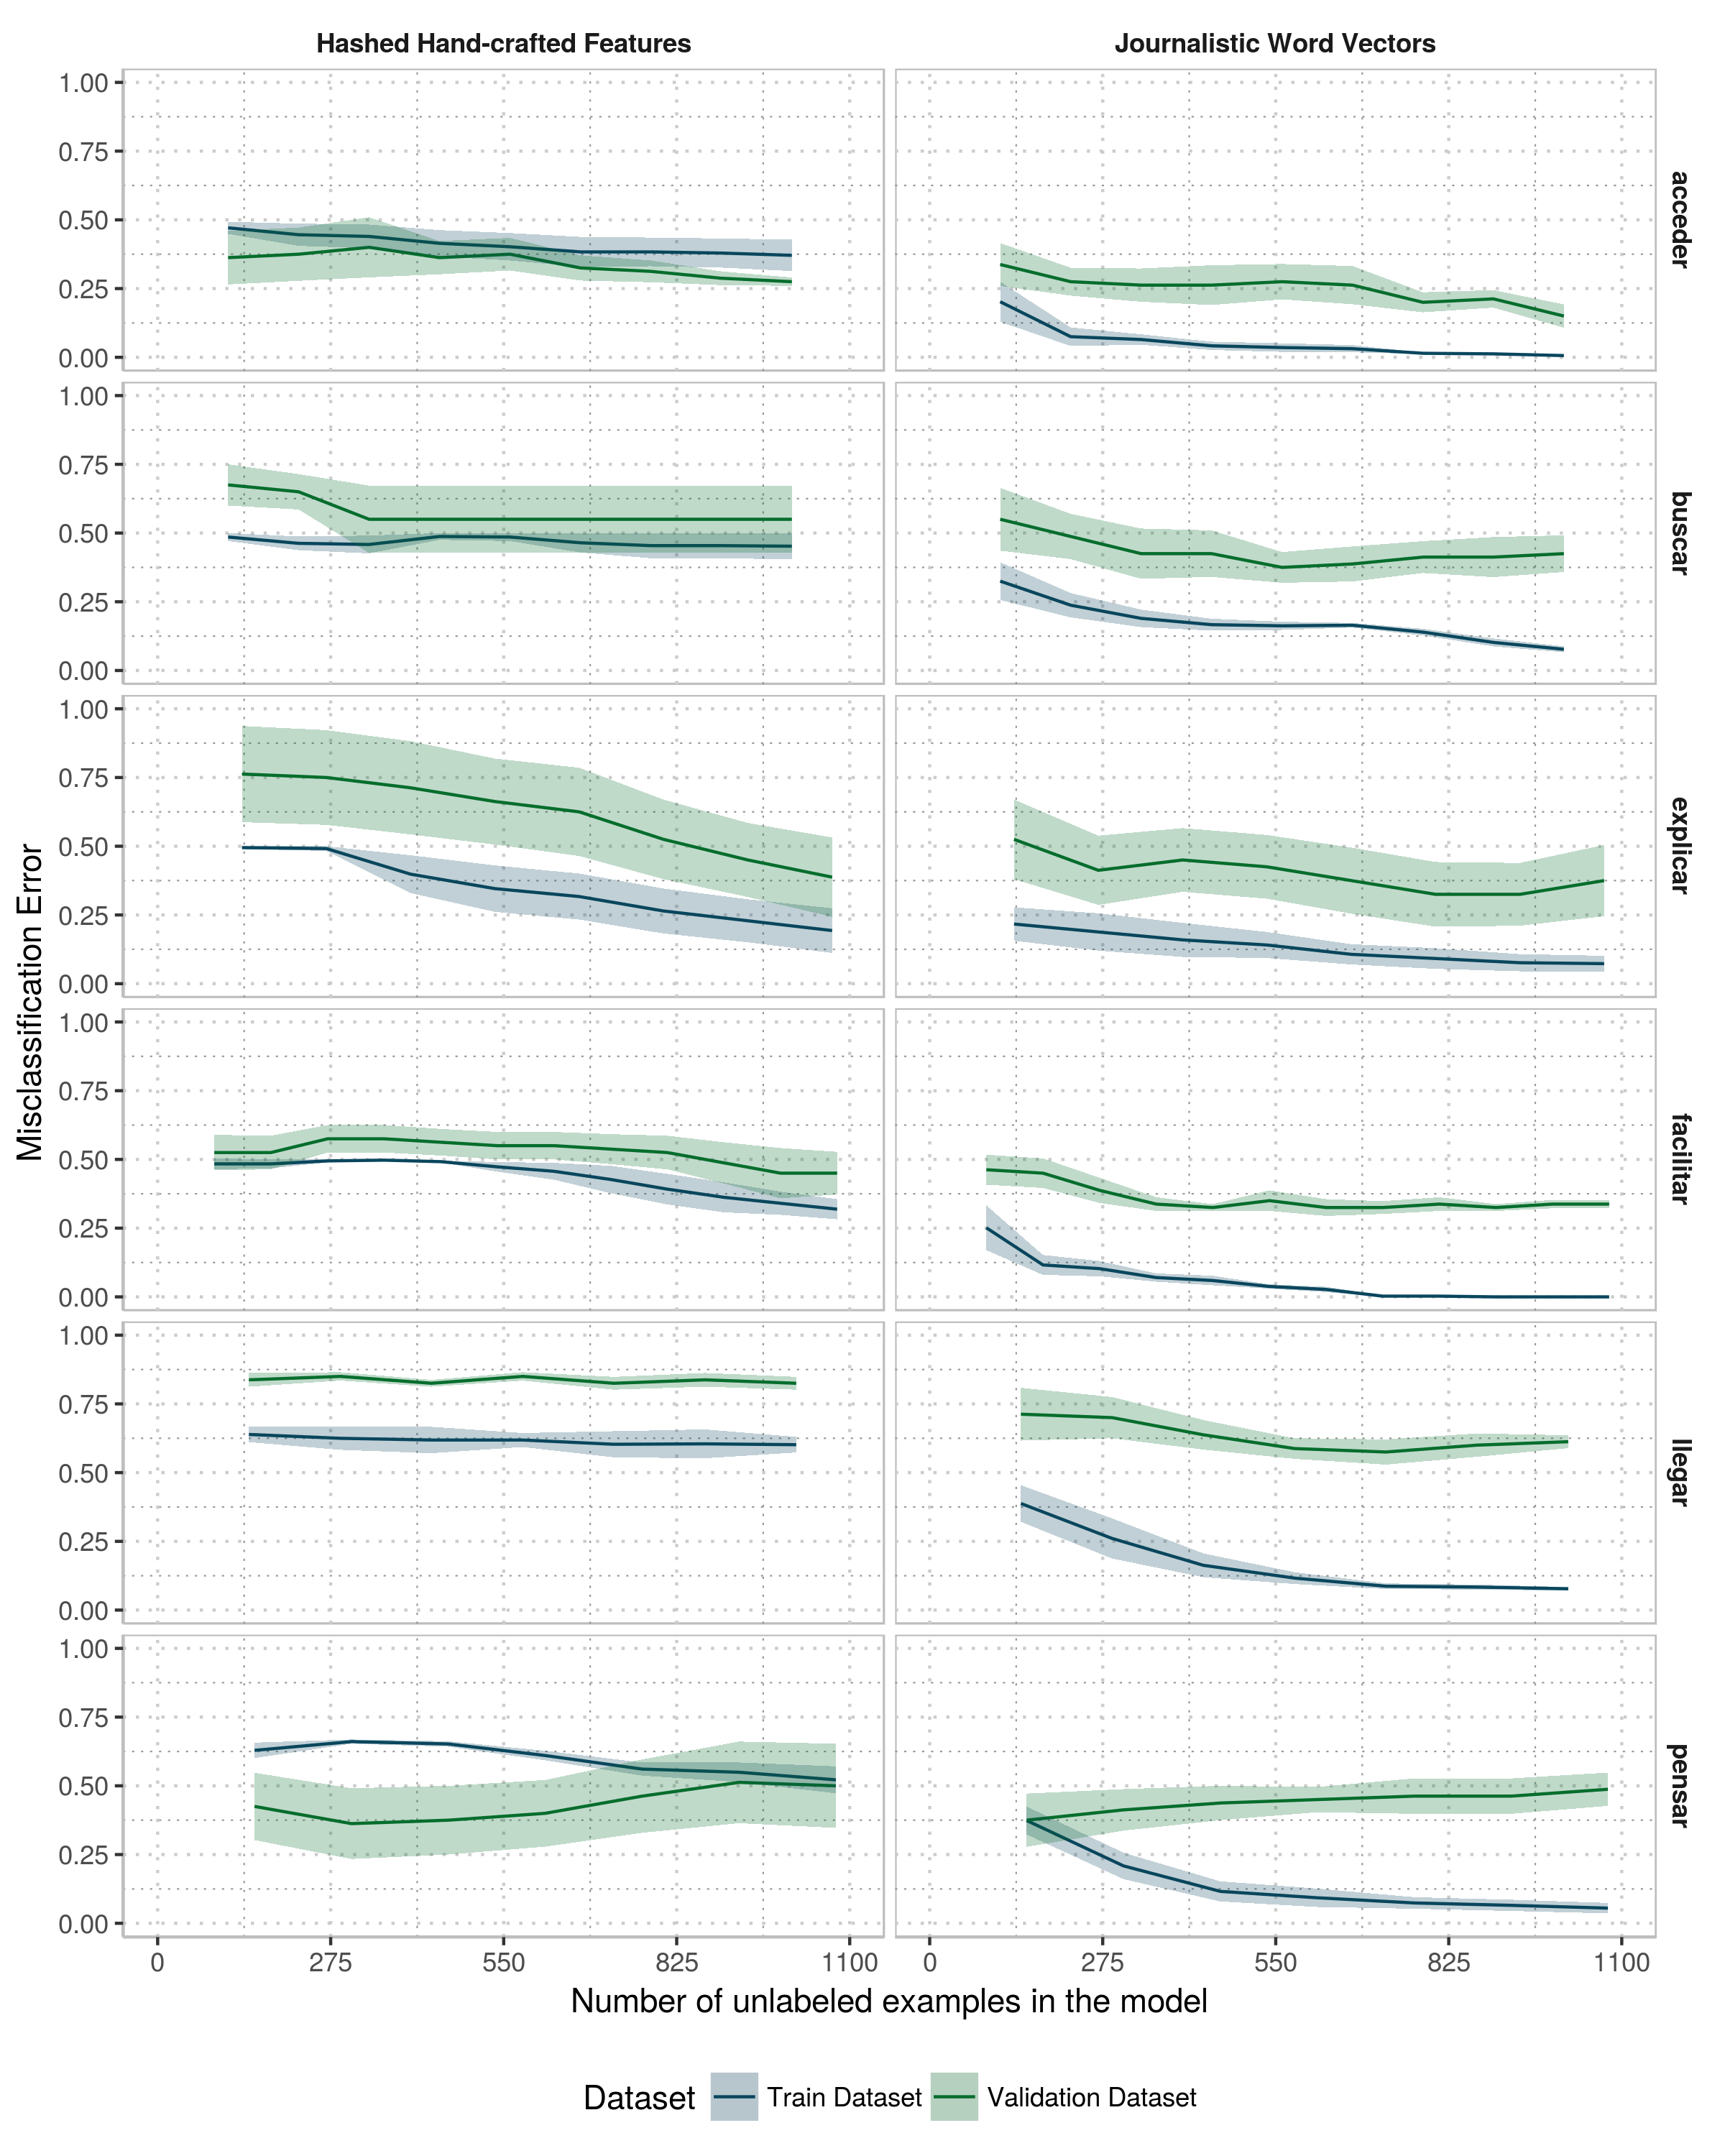
\includegraphics[height=.9\textheight,width=\textwidth,keepaspectratio]
    {plots/ladder/overfit_measure_per_examples}
  \caption{Learning curve as a function of the number of unlabeled examples
  added by the ladder network algorithm in each training iteration}
  \label{fig:ladder:overfit}
\end{figure}

Figure \ref{fig:ladder:overfit} shows the learning curve plot as a function of
the number of examples of the training dataset. The structure of the learning
curve plot is as follows:

\begin{itemize}
  \item Each row shows the results for a token lemma: ``acceder'', ``buscar'',
    ``explicar'', ``facilitar'', ``llegar'', and ``pensar''.
  \item Each column stands for a feature representation: hand-crafted hashed
    features and journalistic word vectors.
  \item The x-coordinate axis represents the number of unlabeled examples added
    in each successive iteration by the ladder networks algorithm.
  \item The y-coordinate axis represents the misclassification error.
  \item There are two colors representing the datasets: training and validation
    (in this case, the validation set).
  \item The solid darker lines represent the mean of misclassification error
    through the different iterations of the datasets over all the models.
  \item The shadowed area, which has a lighter color, represents the standard
    error of the mean of the misclassification error.
\end{itemize}

Remember that in this case, the Experiment stops once all the unlabeled dataset
is traversed once. As the batch size is equal to the number of labeled
instances, which are around $100$ instances per lemma and the maximum number of
unlabeled data is $1000$, then the algorithm stops near iteration number 10,
because it already covers all the unlabeled data by that iteration.

The figure shows a very different picture of what similar plots for other
approaches have shown so far. Unlike what happened for supervised or other
semi-supervised methods, the misclassification error of the training dataset is
not close to zero this time. In this case, the classification error drops
slowly and in most of the cases it is accompanied by the validation error.
There is however more error due to variance (represented by the wider shadowed
area) of the validation dataset. However it seems to be slowly decreasing as
more unlabeled examples are added to the model. Also, except perhaps for the
last two lemmas, the validation error slowly converges to the training error as
well.

Handcrafted features seem to have larger error due to variance than word
embeddings. As seen through this thesis, this looks like a product of the
difficulty of hand-crafted features being to generalize over their domain bias.
Word embeddings, being smoother, model the data in a more generalized way.

It is important to notice that, no matter the representation, the error
progression for most of the cases is quite uniform, that is, even if the
training error is smaller than the validation error, the way both progress is
similar. Moreover, as the ladder network model is adding unlabeled data to help
the network generalize better, from these results it seems that in many cases
it does so precisely by avoiding a huge drop in the error of the training data
whilst having a larger error of the validation data. Once again, this is also
dependant on the lemma, as each lemma has its own set of properties. These
experiments were done on a limited unlabeled corpus due to time and resource
constrains, a future line of work would be to explore the learning curve of the
algorithm with a much larger number of unannotated examples.

The evidence shown by these results is enough to accept Hypothesis
\ref{hyp:ladder:3} that the use of unlabeled data prevents the model to
overfit.

\section{Conclusions}\label{sec:ladder:conclusions}

In this chapter I presented a joint semi-supervised method that, to my
knowledge, had no previous applications in the area of \wsd: the ladder
network.

The experiments and results shown in this chapter have proven very interesting
for its implications and its possibilities in the area of Spanish \vsd, but
also as a general semi-supervised method, applicable to many different areas.

The ladder network is a semi-supervised algorithm that uses a cost function
which is a combination of the supervised cost function given by a feed-forward
neural network (in this case a multilayer perceptron) and an unsupervised cost
function that results in the layer by layer reconstruction of an autoencoder.
The first is used to train on labeled data while the second is used to train on
unlabeled data. The use of a cost functions that has an unsupervised part in
the training of the classifier helps smoothing the fitting of the labeled data
in the same network.

As a consequence, the ladder network improves on other methods by overcoming
some of the shortcomings they had. By integrating an unlabeled dataset it has
more coverage than a purely supervised method. It also has better performance
than self-learning because it keeps under control the bias to the most frequent
class. Finally, it is cheaper than active learning by avoiding the need for a
human annotator to add new examples to the training dataset.

Hypothesis \ref{hyp:ladder:1} states that the ladder network model improves
over purely supervised methods and other semi-supervised methods. The
hypothesis is accepted as shown by the results of Section
\ref{sec:ladder:hyp:1}. The experiments reported that the ladder network
effectively reached the performance of other methods such as active learning or
purely supervised, and in some cases it even outperformed them. What was most
important from these results was to see how ladder networks could sacrifice
some performance in the most frequent class to better represent the less
frequent classes given the right conditions (i.e. stopping at 25 iterations).
Moreover, ladder networks could perform better in senses that the supervised
approach could not recognize at all in the test corpus. Even if the ladder
network could not perform as well as active learning in some cases, it is still
important to note that ladder networks do not rely on a human for the
unsupervised part.

Hypothesis \ref{hyp:ladder:2} was partially accepted. The hypothesis stated
that if the model was used to automatically annotate instances from an
unlabeled corpus, the representativity of the classes in those instances would
be maintained. The results of Section \ref{sec:ladder:hyp:2} show how the
distribution of the classes evolved across iterations. In these results, the
number of iterations also had an important effect on the outcome, as I
explained that when running the algorithm for 100 iterations it was around
iteration number 25 that the model began to drift to the most frequent class.
This is why I decided to truncate the models at 25 iterations and compare the
results. These results showed that for hand-crafted features the Hypothesis
could not be accepted as it was too extreme. In each iteration, the
hand-crafted features model would mark all the unlabeled examples as being part
of only one class, first the less frequent classes and eventually the most
frequent one. However, the model based on word embeddings did show better
results in line with what Hypothesis \ref{hyp:ladder:2} stated. In the latter,
the representativity of the classes was more uniformly maintained through the
iterations. A line of future work would be to use the difference between the
original corpus's distribution and the distribution of the predicted batch
as a stopping criterion, similar to the work by Zhao et al. \cite{Zhao:2017aa}.

Hypothesis \ref{hyp:ladder:3} stated that the use of unlabeled data helps the
ladder network model reduce the tendency to overfit. I discussed the results of
the experiments regarding this hypothesis in Section \ref{sec:ladder:hyp:3}.
In previous chapters I explored how the learning curve evolved by adding
labeled data to the model. In this case however I decided to explore how adding
unlabeled data to the model impacts on the tendency to overfit of the model.
Even if it was not directly comparable to what I have seen in previous
chapters, the basic idea of seeing the tendency to overfit is the same: how new
information on the model affects the way it takes decisions. The results showed
that the learning curve kept uniform while unlabeled data was added to the
model. Both training error and validation error slowly dropped over time for
most of the lemmas, and the error due to variance was reduced as well.

The results of this chapter show the potential ladder networks have as a
semi-supervised approach, not only for Spanish \vsd, but as a method in
general. There is still work to be done regarding this method.

In future work, the first line would be to explore how the learning curve
evolves when it is not limited to a limited number of unlabeled instances. The
ideal approach would be to have an online learning \cite{bottou-98x} method
where new unsupervised data could be added indefinitely. 

Another line of work would be to do a manual evaluation of the automatically
annotated instances and compare that to what self-learning does. Finally, as
this method is an algorithm on its own right, it could be used along some of
the previous wrapper methods. It would be interesting then to see how a
combination of the ladder network wrapped by active learning would evolve.

Regarding the customization of the ladder network algorithm, there is plenty
future work to do: the exploration of different types of combination functions,
the use of other types of neural networks such as recurrent or convolutional,
and the design of a more end-to-end approach that holds the ladder network as
its core.


\part{Conclusions}\label{chapter:conclusions}

\chapter{Conclusions}
\section{Contributions}

The experimentation of this thesis showed that the lack of data produces a
tendency to overfit in purely supervised learning models, together with small
coverage. To tackle these problems I explored different semi-supervised
methods, each one with advantages and disadvantages on their own. The {\em
ladder network} model was found the most promising one in terms of taking
advantage of the unlabeled data to improve the performance of purely supervised
models.

My proposed goal for this thesis was to study how different semi-supervised
techniques could improve a task that would greatly benefit from them.
Throughout the experiments and results of this work I researched on the
properties, benefits, and shortcomings of different semi-supervised approaches
on a particular task. To select the task I decided to explore a domain which
would effectively find it useful the use of a semi-supervised technique. I did
not want just to use some toy dataset on which the properties of
semi-supervised learning would apply just because it was designed to have such
results. What I was interested in was a task that had its own set of
challenges, and in particular, a task that had already the ideal setting which
would make semi-supervised learning an logical solution: the task should have a
small amount of labeled data, good enough for a baseline solution, and large
amount of unlabeled data.

Word sense disambiguation, as discussed in the introduction of this work, is a
fundamental task in the field of natural language processing. It is what is
known as an intermediate task, needed for more complex tasks such as machine
translation or information extraction. In particular, the task of \vsd is
useful in relation extraction, as a verb is the lexical piece that establishes
the relations betwen the participants in a sentence. My particular interest
inside the area of \vsd was the area of Spanish \vsd. In this area there has
been only minimial previous work, as most of the work in disambiguation is for
nouns. In particular, I was interested in the task of Spanish \vsd~because of
the availability of the SenSem corpus, which is a manually disambiguated corpus
for Spanish verbs. This resource gives a supervised baseline and the initial
seed needed for semi-supervised methods. On the other hand, the resources
available for unlabeled data are more than enough for the unsupervised part of
the semi-supervised tasks.

Chapter \ref{chapter:supervised} starts by exploring the different supervised
algorithms to bring their shortcomings into focus and plan how I could address
them as challenges. The chapter does a research on different techniques using
what I called {\em hand-crafted features}, i.e. features taken from the labeled
corpus itself. First, the chapter's main focus was to set a common ground for
the experimentation avoiding an exponential explosion of possible experiments
and results that would have become impossible to analyze and draw conclusions
from.  This starting point was set to explore different ways of representing
the data and to reduce the resources consumed by those representations using
dimensionality reduction techniques. The chapter then explores also different
classifiers, linear and non-linear, to rule out big differences before
selecting one of them. Once the base structure of the experiments is set, the
chapter explores how the number of labeled data in a model can impact on the
final performance of the model. What the experimentation results show is that
the main problem of the supervised approach is the lack of labeled data to
train a good model that can generalize well. In particular, the model is
trained over a labeled dataset of a specific domain, which makes the challenge
of overfitting even worse. On the other hand, the model has little information:
the coverage is greatly affected by the few available examples to train. Once
the results of this chapter were clear, in successive chapters I explored the
impact of different semi-supervised learning techniques on these two
challenges: overfitting of the model in the training dataset, and coverage of
the model by adding more information from new examples.

Chapter \ref{chapter:embeddings} introduced the use of {\em word embeddings} as
an alternative representation of the instances used to train the classifier.
This is known as {\em disjoint semi-supervised learning}, where an unsupervised
task is performed previously (i.e. training word embeddings) and the result of
this task is integrated into a supervised task (i.e. \vsd). This chapter
explored how the use of word embeddings impacts on a supervised classifier. In
particular, the chapter experimented on different types of word embeddings
trained with different domains. Those embeddings trained on the same domain as
the labeled dataset (i.e. journalistic domain) improve the performance of the
supervised classifier. However, the supervised classifier trained with word
embeddings representations did not reach the performance levels of the model
trained with hand-crafted features. Although this could be interpreted as a
problem, successive chapters show the contrary. The purely supervised model
obtained better performance figures than the model based on word embeddings
because hand-crafted features were closer to the data, thus having a higher
tendency to overfit. Other experiments in this chapter and the analysis of
results showed that, in contrast, word embeddings are a good representation to
reduce the model's tendency to overfit the training data. This is more strongly
supported by evidence in Chapter \ref{chapter:self-learning}, with experiments
in a more general corpus.

Chapter \ref{chapter:self-learning} was the first to introduce a {\em joint
learning} algorithm in which both the labeled and the unlabeled dataset
contribute to the task of semi-supervised learning. The chapter explores {\em
self-learning}, a wrapper algorithm over a supervised classifier. In this
scheme, the labeled dataset serves as an initial seed to train a base model for
a classifier. This classifier is used to augment the information available in
the model by automatically annotating new instances from an unlabeled dataset
based on certainty and adding them as labeled instances to train a new model.
This process is repeated iteratively to have more and more training examples
taken from the unlabeled data. The experiments in this chapter explored how
this new data affected the performance of the model. In particular, I wanted
to see how the new data effectively increased the initial model with more
information gathered from the new instances. This new information could help
expanding the model's coverage. Adding new examples of a new dataset would also
help the model prevent the tendency to overfit. However, what I found was that
the expansion of the model's coverage was done at expense of the quality of the
model. The self-learning algorithm had problems specially when dealing with a
largely unbalanced dataset, that is, with a clearly majority class. This
configuration is common in a task such as Spanish \vsd, as well as for any \nlp
task, because of the Zipfian distribution of natural language itself. Then,
while more information seems to be added to the model, what is actually
happening is that the model is drifting to classify new data almost exclusively
as part of the most frequent class in the dataset. Then, the model did not
actually expand its coverage, but it was just blurring the decision boundaries
of the original supervised classifier. From this chapter however there was an
important finding given by the general results and performance obtained with
word embeddings. These last were proven to behave much better than hand-crafted
features. They represented minority classes better, mitigating the drift to the
majority class. As they are trained from a more general domain than
hand-crafted features, they also dealt better with the change of domain given 
by the unlabeled instances the self-learning algorithm used to expand the 
supervised model.

Chapter \ref{chapter:active} explored a second joint learning technique: {\em
active learning}. Like self-learning, this is also al wrapper algorithm. It
trains based on an initial seed and then adds examples from an unlabeled pool
of available instances. These instances serve to augment the pool of labeled
examples which are used to train a new model which is used again to fetch new
data to add. The main difference between this algorithm and self-learning is
the way the unlabeled dataset is annotated. In self-learning the annotation is
automatic, and automatically annotated instances are included as training if
the classifier has high confidence over the instance. In contrast, active
learning uses a human (generally a domain expert) to annotate unlabeled
examples selected in an ``intelligent'' way. This means instances should be
those which, once annotated, have the largest impact on the new model,
increasing its certainty or reducing error. The experimentation done for this
chapter was merely exploratory, because the active learning approach is by
itself an expensive method that requires manual annotation. However, results
were promising enough to have some insights on how this method could help
improve the task of Spanish \vsd. The results of the chapter were interesting
because the model not only improved on the most frequent classes but also in
the less frequent classes as well. Moreover, because of the algorithm's way to
select instances for annotation, it did not suffer from the drifting to the
most frequent class that self-learning showed. Indeed, active learning was
shown to increase the model's information with less examples provided in
comparison.  But, as it requires a human annotator in order to work, active
learning becomes an expensive approach for semi-supervised learning.

Finally, chapter \ref{chapter:ladder} explored a fairly new semi-supervised
learning technique: {\em the ladder network}. In this neural network, the
architecture is designed to train the parameters by optimizing a cost function
that is a combination of a supervised cost function and an unsupervised cost
function. The neural network has an architecture that resembles that of an
autoencoder, with an encoder and a decoder paths. The encoder path is given by
a feed-forward neural network with an output layer that is trained by using a
supervised cost function. The decoder path is used to reconstruct the training
instances and thus helps smooth the neural network by avoiding overfitting to a
small supervised dataset. In this model the unlabeled examples are not tagged
and added to the model as in previous algorithms. Still, unlabeled instances
still help to expand the coverage of the model as the information they provide
is integrated to that of the labeled dataset. The experiments in this chapter
explored the use of ladder networks as an alternative semi-supervised approach
that overcomes the shortcoming of self-learning that adds new instances only as
if they were part of the most frequent class. Also, the ladder network model
overcomes the problem of active learning, that is, the cost of manual
annotation. The results of the chapter were promising as the ladder network had
good performance results, not only in the most frequent class but in all
classes in general. Very often it surpassed the results obtained by a purely
supervised approach or active learning. The use of unlabeled data to help
training the model added more information which would help to expand the
coverage of the model. Moreover, the model proved to be able to avoid
overfitting as the unlabeled examples and the unsupervised cost function
prevented the supervised part to overfit the labeled data. Ladder networks
showed impressive results coming from a purely automatic process for
semi-supervised learning and is a good candidate to keep exploring.

\section{Future Work}

The main obstacle through the experiments done in this thesis was the
unbalanced dataset. The presence of a majority class which unbalanced the
distribution of the classes is something common for a task in natural language
processing. This unbalance had great impact in how the semi-supervised
techniques could work their way in the task of Spanish \vsd. As I saw in
Chapter \ref{chapter:self-learning}, the problem of unbalance, even if it was
small at the beginning, can quickly grow and end up hitting on the algorithm's
quality, making the final model useless. Unbalanced classes is a problem on its
own right, that I could not cover more thoroughly in this work.  There are
techniques, besides oversampling or undersampling, which help dealing with this
kind of situations and that would require further exploration in future work.
However, the best approach so far to deal with the problem of unbalance and
bias to the most frequent class was given by active learning with uncertainty
sampling, which by design would tend to add those instances the model had less
information about, i.e. the less frequent classes.

The domain of the labeled corpus also had a great impact in the experiments and
results I analyzed through this thesis. The labeled corpus was the base
resource to work with in this thesis and as such the quality of the resource
impacted directly on how good the models could be. It is important to note that
as it was a heavily domain-based resource, it could also obscure some of the
results, e.g. when it showed a better performance for the hand-crafted features
than the word embeddings just because the latter generalized better. This put
in consideration how I interpret the results: a model that shows a drop in
performance in comparison to another model is not automatically a bad model.
Sometimes there are other metrics and other views of the data that help
identify what a model is leaving out in order to gain performance, for example,
representativity of minority classes or better generalization to data from
other domains. Also, the heavy influence on the domain showed the importance of
having more heterogeneous data in order to seek a good model. Indeed,
semi-supervised learning techniques, which acquired information from a corpus
from a general domain, improved some aspects of the original model, which was
too close to the labeled dataset.

The two main challenges tackled in this work were coverage, observed as the
information actionable by the model, as well as tendency to overfit or
generalize. These challenges were direct results of having a small amount of
labeled data and such data being part of a very specific domain.
Semi-supervised techniques were explored in order to overcome these two
challenges. It is left for future work to carry out experiments that are more
driven by the domain and see how the domain really affects the final results
when exploring other domains. For example, it is interesting to explore how the
use of unlabeled data from the same domain or a contrasting domain affects
semi-supervised models.

With more resources available, some of the most important future work I have is
the use of larger unlabeled corpora with different semi-supervised techniques.
This ranges from training word embeddings with more corpora coming from
different resources available online, to the use of more unlabeled training
instances in the ladder network. For active learning, the manual annotation was
done mostly by me with the help of my thesis supervisor, but it would benefit
of a domain expert that could also work with more examples than the very little
amount I could manage to annotate manually. Finally, I would like to do the
analysis on more of the available lemmas, as due to time constraints I could
only explore a small sample of all the available possibilities the area of
Spanish \vsd~has to offer. With more resources as well, I will also work on a
more thorough error analysis of the experiments, specially those regarding
overfitting and distribution of classes. I am most interested in seeing how
semi-supervised models deal with the annotation of new examples by doing a
manual evaluation on examples myself, specially for the cases of self-learning
and ladder networks.

Finally, in a more technical approach, future work is left for exploring
different combinations of the semi-supervised techniques such as the use of a
combined algorithm between self-learning and active learning or moreover using
a combination of one of the wrapper algorithms with the ladder network itself.
In particular, the ladder network is a very promising approach that would
require further exploration to tune its components. A line of future work would
be to use the difference between the original corpus's distribution and the
distribution of the predicted batch as a stopping criterion. Also, many of the
hyperparameters can be modified trying to reach better performance of the
algorithm in the task: from the denoising cost weights to the architecture of
the encoder layer, also changing the combinator function given by the authors.
Still, the most interesting line of work on ladder networks would be to check
how they work by integrating a more complex neural network than just a plain
multilayer perceptron. It would be interesting to see how a ladder network
constructed over a convolutional neural network or a recurrent neural network
can help the final performance of the models. In general terms, ladder
networks, being the most novel approach studied in this thesis, gives ample
room for improvement and exploration.


%----------------------------------------------------------------------------------------
%	THESIS CONTENT - APPENDICES
%----------------------------------------------------------------------------------------

\appendix % Cue to tell LaTeX that the following "chapters" are Appendices

% Include the appendices of the thesis as separate files from the Appendices folder
% Uncomment the lines as you write the Appendices

%\include{Appendices/AppendixA}
%\include{Appendices/AppendixB}
%\include{Appendices/AppendixC}

%----------------------------------------------------------------------------------------
%	BIBLIOGRAPHY
%----------------------------------------------------------------------------------------

\bibliographystyle{apalike}
\bibliography{thesis_bibliography}

%----------------------------------------------------------------------------------------

\end{document}  
